% Options for packages loaded elsewhere
\PassOptionsToPackage{unicode}{hyperref}
\PassOptionsToPackage{hyphens}{url}
%
\documentclass[
]{book}
\usepackage{amsmath,amssymb}
\usepackage{iftex}
\ifPDFTeX
  \usepackage[T1]{fontenc}
  \usepackage[utf8]{inputenc}
  \usepackage{textcomp} % provide euro and other symbols
\else % if luatex or xetex
  \usepackage{unicode-math} % this also loads fontspec
  \defaultfontfeatures{Scale=MatchLowercase}
  \defaultfontfeatures[\rmfamily]{Ligatures=TeX,Scale=1}
\fi
\usepackage{lmodern}
\ifPDFTeX\else
  % xetex/luatex font selection
\fi
% Use upquote if available, for straight quotes in verbatim environments
\IfFileExists{upquote.sty}{\usepackage{upquote}}{}
\IfFileExists{microtype.sty}{% use microtype if available
  \usepackage[]{microtype}
  \UseMicrotypeSet[protrusion]{basicmath} % disable protrusion for tt fonts
}{}
\makeatletter
\@ifundefined{KOMAClassName}{% if non-KOMA class
  \IfFileExists{parskip.sty}{%
    \usepackage{parskip}
  }{% else
    \setlength{\parindent}{0pt}
    \setlength{\parskip}{6pt plus 2pt minus 1pt}}
}{% if KOMA class
  \KOMAoptions{parskip=half}}
\makeatother
\usepackage{xcolor}
\usepackage{color}
\usepackage{fancyvrb}
\newcommand{\VerbBar}{|}
\newcommand{\VERB}{\Verb[commandchars=\\\{\}]}
\DefineVerbatimEnvironment{Highlighting}{Verbatim}{commandchars=\\\{\}}
% Add ',fontsize=\small' for more characters per line
\usepackage{framed}
\definecolor{shadecolor}{RGB}{248,248,248}
\newenvironment{Shaded}{\begin{snugshade}}{\end{snugshade}}
\newcommand{\AlertTok}[1]{\textcolor[rgb]{0.94,0.16,0.16}{#1}}
\newcommand{\AnnotationTok}[1]{\textcolor[rgb]{0.56,0.35,0.01}{\textbf{\textit{#1}}}}
\newcommand{\AttributeTok}[1]{\textcolor[rgb]{0.13,0.29,0.53}{#1}}
\newcommand{\BaseNTok}[1]{\textcolor[rgb]{0.00,0.00,0.81}{#1}}
\newcommand{\BuiltInTok}[1]{#1}
\newcommand{\CharTok}[1]{\textcolor[rgb]{0.31,0.60,0.02}{#1}}
\newcommand{\CommentTok}[1]{\textcolor[rgb]{0.56,0.35,0.01}{\textit{#1}}}
\newcommand{\CommentVarTok}[1]{\textcolor[rgb]{0.56,0.35,0.01}{\textbf{\textit{#1}}}}
\newcommand{\ConstantTok}[1]{\textcolor[rgb]{0.56,0.35,0.01}{#1}}
\newcommand{\ControlFlowTok}[1]{\textcolor[rgb]{0.13,0.29,0.53}{\textbf{#1}}}
\newcommand{\DataTypeTok}[1]{\textcolor[rgb]{0.13,0.29,0.53}{#1}}
\newcommand{\DecValTok}[1]{\textcolor[rgb]{0.00,0.00,0.81}{#1}}
\newcommand{\DocumentationTok}[1]{\textcolor[rgb]{0.56,0.35,0.01}{\textbf{\textit{#1}}}}
\newcommand{\ErrorTok}[1]{\textcolor[rgb]{0.64,0.00,0.00}{\textbf{#1}}}
\newcommand{\ExtensionTok}[1]{#1}
\newcommand{\FloatTok}[1]{\textcolor[rgb]{0.00,0.00,0.81}{#1}}
\newcommand{\FunctionTok}[1]{\textcolor[rgb]{0.13,0.29,0.53}{\textbf{#1}}}
\newcommand{\ImportTok}[1]{#1}
\newcommand{\InformationTok}[1]{\textcolor[rgb]{0.56,0.35,0.01}{\textbf{\textit{#1}}}}
\newcommand{\KeywordTok}[1]{\textcolor[rgb]{0.13,0.29,0.53}{\textbf{#1}}}
\newcommand{\NormalTok}[1]{#1}
\newcommand{\OperatorTok}[1]{\textcolor[rgb]{0.81,0.36,0.00}{\textbf{#1}}}
\newcommand{\OtherTok}[1]{\textcolor[rgb]{0.56,0.35,0.01}{#1}}
\newcommand{\PreprocessorTok}[1]{\textcolor[rgb]{0.56,0.35,0.01}{\textit{#1}}}
\newcommand{\RegionMarkerTok}[1]{#1}
\newcommand{\SpecialCharTok}[1]{\textcolor[rgb]{0.81,0.36,0.00}{\textbf{#1}}}
\newcommand{\SpecialStringTok}[1]{\textcolor[rgb]{0.31,0.60,0.02}{#1}}
\newcommand{\StringTok}[1]{\textcolor[rgb]{0.31,0.60,0.02}{#1}}
\newcommand{\VariableTok}[1]{\textcolor[rgb]{0.00,0.00,0.00}{#1}}
\newcommand{\VerbatimStringTok}[1]{\textcolor[rgb]{0.31,0.60,0.02}{#1}}
\newcommand{\WarningTok}[1]{\textcolor[rgb]{0.56,0.35,0.01}{\textbf{\textit{#1}}}}
\usepackage{longtable,booktabs,array}
\usepackage{calc} % for calculating minipage widths
% Correct order of tables after \paragraph or \subparagraph
\usepackage{etoolbox}
\makeatletter
\patchcmd\longtable{\par}{\if@noskipsec\mbox{}\fi\par}{}{}
\makeatother
% Allow footnotes in longtable head/foot
\IfFileExists{footnotehyper.sty}{\usepackage{footnotehyper}}{\usepackage{footnote}}
\makesavenoteenv{longtable}
\usepackage{graphicx}
\makeatletter
\def\maxwidth{\ifdim\Gin@nat@width>\linewidth\linewidth\else\Gin@nat@width\fi}
\def\maxheight{\ifdim\Gin@nat@height>\textheight\textheight\else\Gin@nat@height\fi}
\makeatother
% Scale images if necessary, so that they will not overflow the page
% margins by default, and it is still possible to overwrite the defaults
% using explicit options in \includegraphics[width, height, ...]{}
\setkeys{Gin}{width=\maxwidth,height=\maxheight,keepaspectratio}
% Set default figure placement to htbp
\makeatletter
\def\fps@figure{htbp}
\makeatother
\setlength{\emergencystretch}{3em} % prevent overfull lines
\providecommand{\tightlist}{%
  \setlength{\itemsep}{0pt}\setlength{\parskip}{0pt}}
\setcounter{secnumdepth}{5}
\usepackage{booktabs}
\ifLuaTeX
  \usepackage{selnolig}  % disable illegal ligatures
\fi
\usepackage[]{natbib}
\bibliographystyle{plainnat}
\IfFileExists{bookmark.sty}{\usepackage{bookmark}}{\usepackage{hyperref}}
\IfFileExists{xurl.sty}{\usepackage{xurl}}{} % add URL line breaks if available
\urlstyle{same}
\hypersetup{
  pdftitle={Intermediate Quantitative Methods},
  pdfauthor={Lucas Lemmann},
  hidelinks,
  pdfcreator={LaTeX via pandoc}}

\title{Intermediate Quantitative Methods}
\author{Lucas Lemmann}
\date{2023-12-11}

\begin{document}
\maketitle

{
\setcounter{tocdepth}{1}
\tableofcontents
}
\hypertarget{about}{%
\chapter*{About}\label{about}}
\addcontentsline{toc}{chapter}{About}

What is this book about? What for?

\hypertarget{how-to-use-these-exercises}{%
\section{How to use these exercises?}\label{how-to-use-these-exercises}}

\begin{itemize}
\tightlist
\item
  Besides the 14 lectures, the course will be organized around 12 non-graded exercises:

  \begin{itemize}
  \tightlist
  \item
    5 labs
  \item
    7 do-it-yourself (DIYS)
  \end{itemize}
\item
  The labs' solutions will be discussed in detail between TAs and students in the corresponding sessions, while DIYS will not. In both cases, we will publish the solutions the week after the exercise is due.
\item
  We encourage you to prepare for the lab sessions in advance as well as to attend them to discuss any doubts they might have related to the labs material.
\item
  To prevent redundant communications (i.e., emails with the same information), share your questions regarding the exercises in the forum. Labs will emphasize the most voted questions.
\item
  While we encourage and foster a collaborative learning process, we expect you to work individually first.

  \begin{itemize}
  \tightlist
  \item
    I.e., try to address the task on your own first, identify what is limiting you, try to solve it on your own (not for too long), and, if you cannot find a solution, reach out your classmates. Once you find your solution, consider discussing the solution with your classmates.
  \end{itemize}
\item
  All the files behind this book can be found in its GitHub repository.
\end{itemize}

\hypertarget{schedule}{%
\section{Schedule}\label{schedule}}

\begin{longtable}[]{@{}ccc@{}}
\toprule\noalign{}
Week & Dates & Exercise type \\
\midrule\noalign{}
\endhead
\bottomrule\noalign{}
\endlastfoot
1 & 19-25/02 & DIYS 1 \\
2 & 26/02-03/03 & Lab 1 \\
3 & 04/03-10/03 & Lab 1 \\
4 & 11/03-17/03 & DIYS 2 \\
5 & 18/03-24/03 & Lab 2 \\
6 & 25/03-31/03 & DIYS 3 \\
\textbf{Spring Break} & 28/03-07/04 & None? \\
7 & 08/04-14/04 & Lab 3 \\
8 & 15/04-21/04 & DIYS 4 \\
9 & 22/04-28/04 & Lab 4 \\
10 & 29/04-05/05 & DIYS 5 \\
11 & 06/05-12/05 & Lab 5 \\
12 & 13/05-19/05 & Lab 5 \\
13 & 20/05-26/05 & DIYS 6 \\
14 & 27/05-02/06 & DIYS 7 \\
\end{longtable}

\hypertarget{week-1-diys-1}{%
\chapter{Week 1: DIYS 1}\label{week-1-diys-1}}

\hypertarget{aims}{%
\section{Aims:}\label{aims}}

\begin{enumerate}
\def\labelenumi{\arabic{enumi}.}
\tightlist
\item
  To refresh your R skills.
\item
  Performing some basic analyses (i.e., descriptive, exploratory, and hypothesis testing ones).
\end{enumerate}

\hypertarget{first-part-repetition-rrstudio}{%
\section{First Part: REPETITION R/RStudio}\label{first-part-repetition-rrstudio}}

\begin{enumerate}
\def\labelenumi{\arabic{enumi}.}
\tightlist
\item
  Download the files \texttt{f.txt} and \texttt{m.txt}. They contain information on screentime (i.e., number of seconds per day spent on mobile phone), and closeness to a populist party for female and male individuals respectively. Open them and explore the first 3 observations for each file.
\end{enumerate}

Note: remember that this book was developed as an R-project, which is a way to ensure reproducibility of projects. One of the advantages of R-projects is that files are stored in directories (i.e., folders) that are defined relative to the R-project. For example, if the folder \texttt{Data} is stored in the same folder as the project, files stored in \texttt{Data} can be accessed as follows: \texttt{female\ \textless{}-\ read.table("Data/f.txt",\ header\ =\ TRUE,\ sep\ =\ "\textbackslash{}t")}.To learn more about R-projects, check \href{https://rfortherestofus.com/2022/10/rstudio-projects}{this} entry.

\begin{Shaded}
\begin{Highlighting}[]
\CommentTok{\# Your code goes here}
\end{Highlighting}
\end{Shaded}

{For the exercise before publishing the solution}

\begin{Shaded}
\begin{Highlighting}[]
\CommentTok{\# open data}
\NormalTok{female }\OtherTok{\textless{}{-}} \FunctionTok{read.table}\NormalTok{(}\StringTok{"Data/f.txt"}\NormalTok{, }\AttributeTok{header =} \ConstantTok{TRUE}\NormalTok{, }\AttributeTok{sep =} \StringTok{";"}\NormalTok{)}

\CommentTok{\# explore data}
\FunctionTok{head}\NormalTok{(female, }\DecValTok{3}\NormalTok{)}
\end{Highlighting}
\end{Shaded}

\begin{verbatim}
##   ID ScreenTime ClosenessPopulistParty
## 1  3      15000               1.176471
## 2  4      14861               1.294118
## 3  5      14861               1.294118
\end{verbatim}

\begin{Shaded}
\begin{Highlighting}[]
\CommentTok{\# open data}
\NormalTok{male }\OtherTok{\textless{}{-}} \FunctionTok{read.table}\NormalTok{(}\StringTok{"Data/m.txt"}\NormalTok{, }\AttributeTok{header =} \ConstantTok{TRUE}\NormalTok{, }\AttributeTok{sep =} \StringTok{";"}\NormalTok{)}

\CommentTok{\# explore data}
\FunctionTok{head}\NormalTok{(male, }\DecValTok{3}\NormalTok{)}
\end{Highlighting}
\end{Shaded}

\begin{verbatim}
##   ID ScreenTime ClosenessPopulistParty
## 1  1      15000              0.7361963
## 2  2      15000              0.7361963
## 3  6      14861              0.6748466
\end{verbatim}

Some key functions in dplyr can be categorized as dealing with columns (e.g., \texttt{select}, \texttt{mutate}), rows (e.g., \texttt{filter}, \texttt{distinct}, \texttt{arrange}), or groups (e.g., \texttt{group\_by}, \texttt{summarise}, and \texttt{count}). Let's use some of them!

\begin{enumerate}
\def\labelenumi{\arabic{enumi}.}
\setcounter{enumi}{1}
\tightlist
\item
  Select only the columns `ScreenTime' and `ClosenessPopulistParty'. Do it only for the first three observations of the data on females.
\end{enumerate}

\begin{Shaded}
\begin{Highlighting}[]
\FunctionTok{head}\NormalTok{(female, }\DecValTok{3}\NormalTok{) }\SpecialCharTok{\%\textgreater{}\%}
  \FunctionTok{select}\NormalTok{(ScreenTime, ClosenessPopulistParty)}
\end{Highlighting}
\end{Shaded}

\begin{verbatim}
##   ScreenTime ClosenessPopulistParty
## 1      15000               1.176471
## 2      14861               1.294118
## 3      14861               1.294118
\end{verbatim}

\begin{enumerate}
\def\labelenumi{\arabic{enumi}.}
\setcounter{enumi}{2}
\tightlist
\item
  Select all columns except `ID'. Do not use \texttt{ScreenTime} nor \texttt{ClosenessPopulistParty}. Do it only for the first three observations of the data on females. Is the resulting table the same as the previous point? If not, check your answer.
\end{enumerate}

\begin{Shaded}
\begin{Highlighting}[]
\FunctionTok{head}\NormalTok{(female, }\DecValTok{3}\NormalTok{) }\SpecialCharTok{\%\textgreater{}\%}
  \FunctionTok{select}\NormalTok{(}\SpecialCharTok{{-}}\NormalTok{ID)}
\end{Highlighting}
\end{Shaded}

\begin{verbatim}
##   ScreenTime ClosenessPopulistParty
## 1      15000               1.176471
## 2      14861               1.294118
## 3      14861               1.294118
\end{verbatim}

Note: to check the documentation of \texttt{select}, use \texttt{?select} on the console.

\begin{enumerate}
\def\labelenumi{\arabic{enumi}.}
\setcounter{enumi}{3}
\tightlist
\item
  Use \texttt{mutate} to create a new column in the DataFrame \texttt{female} called \texttt{ScreenTimeTimesClosenessPopulistParty} formed as the product of \texttt{ScreenTime} and \texttt{ClosenessPopulistParty}. Show the first three observations for the new variable.
\end{enumerate}

\begin{Shaded}
\begin{Highlighting}[]
\NormalTok{female }\OtherTok{\textless{}{-}}\NormalTok{female }\SpecialCharTok{\%\textgreater{}\%}
  \FunctionTok{mutate}\NormalTok{(}\AttributeTok{ScreenTimeTimesClosenessPopulistParty=}\NormalTok{ ScreenTime }\SpecialCharTok{*}\NormalTok{ ClosenessPopulistParty)}
  
\FunctionTok{head}\NormalTok{(female}\SpecialCharTok{$}\NormalTok{ScreenTimeTimesClosenessPopulistParty,}\DecValTok{3}\NormalTok{)}
\end{Highlighting}
\end{Shaded}

\begin{verbatim}
## [1] 17647.06 19231.88 19231.88
\end{verbatim}

\begin{enumerate}
\def\labelenumi{\arabic{enumi}.}
\setcounter{enumi}{4}
\tightlist
\item
  Get rid of the column \texttt{ScreenTimeTimesClosenessPopulistParty}. Use \texttt{subset}.
\end{enumerate}

Note: remember to check that the outcome of your code is in accordance with what you expect. To do so, inspect the outcome using \texttt{head}.

\begin{Shaded}
\begin{Highlighting}[]
\NormalTok{female }\OtherTok{\textless{}{-}} \FunctionTok{subset}\NormalTok{(female, }\AttributeTok{select=} \SpecialCharTok{{-}}\NormalTok{ ScreenTimeTimesClosenessPopulistParty)}
\FunctionTok{head}\NormalTok{(female, }\DecValTok{3}\NormalTok{)}
\end{Highlighting}
\end{Shaded}

\begin{verbatim}
##   ID ScreenTime ClosenessPopulistParty
## 1  3      15000               1.176471
## 2  4      14861               1.294118
## 3  5      14861               1.294118
\end{verbatim}

\begin{enumerate}
\def\labelenumi{\arabic{enumi}.}
\setcounter{enumi}{5}
\tightlist
\item
  Use filter to find the share of female individuals with a \texttt{ClosenessPopulistParty} higher than 20 and lower than 21.
\end{enumerate}

\begin{Shaded}
\begin{Highlighting}[]
\NormalTok{f20\_21 }\OtherTok{\textless{}{-}}\NormalTok{ female }\SpecialCharTok{\%\textgreater{}\%}
  \FunctionTok{filter}\NormalTok{(ClosenessPopulistParty}\SpecialCharTok{\textgreater{}}\DecValTok{20}\NormalTok{, ClosenessPopulistParty}\SpecialCharTok{\textless{}}\DecValTok{21}\NormalTok{)}
\end{Highlighting}
\end{Shaded}

The share of female individuals with a \texttt{ClosenessPopulistParty} higher than 20 and lower than 21 is: 0\%.

\begin{enumerate}
\def\labelenumi{\arabic{enumi}.}
\setcounter{enumi}{6}
\tightlist
\item
  Use filter to find the share of female individuals with a \texttt{ClosenessPopulistParty} higher than 20 and lower than 21 while at the same time having less than 14000 \texttt{ScreenTime}.
\end{enumerate}

\begin{Shaded}
\begin{Highlighting}[]
\NormalTok{fClosenessPopulistParty20\_21\_ScreenTime14000 }\OtherTok{\textless{}{-}}\NormalTok{ female }\SpecialCharTok{\%\textgreater{}\%}
  \FunctionTok{filter}\NormalTok{(ClosenessPopulistParty}\SpecialCharTok{\textgreater{}}\DecValTok{20}\NormalTok{, ClosenessPopulistParty}\SpecialCharTok{\textless{}}\DecValTok{21}\NormalTok{, ScreenTime}\SpecialCharTok{\textless{}}\DecValTok{14000}\NormalTok{)}
\end{Highlighting}
\end{Shaded}

The share of female individuals with a \texttt{ClosenessPopulistParty} higher than 20 and lower than 21 while at the same time having less than 14000 is:``, nrow(fClosenessPopulistParty20\_21\_ScreenTime14000)*100/nrow(female)

\begin{enumerate}
\def\labelenumi{\arabic{enumi}.}
\setcounter{enumi}{7}
\tightlist
\item
  Use filter to find the share of male individuals with \texttt{ID} number lower than 5 \textbf{and} higher than 860. Notice that you can use either \texttt{\&} between conditions or simply a comma. Could any dataset generate a different answer? Why?
\end{enumerate}

\begin{Shaded}
\begin{Highlighting}[]
\NormalTok{m\_5\_860 }\OtherTok{\textless{}{-}}\NormalTok{ male }\SpecialCharTok{\%\textgreater{}\%}
  \FunctionTok{filter}\NormalTok{(ID}\SpecialCharTok{\textless{}}\DecValTok{5} \SpecialCharTok{\&}\NormalTok{ ID}\SpecialCharTok{\textgreater{}}\DecValTok{860}\NormalTok{)}
\end{Highlighting}
\end{Shaded}

The share of male individuals with \texttt{ID} number lower than 5 AND higher than 860 is: 0

\begin{enumerate}
\def\labelenumi{\arabic{enumi}.}
\setcounter{enumi}{8}
\tightlist
\item
  Use filter to find the share of male individuals with \texttt{ID} number lower than 5 \textbf{or} higher than 860. Use \texttt{\textbar{}} between conditions. Could any dataset generate a different answer? Why?
\end{enumerate}

\begin{Shaded}
\begin{Highlighting}[]
\NormalTok{m\_5\_or\_860 }\OtherTok{\textless{}{-}}\NormalTok{ male }\SpecialCharTok{\%\textgreater{}\%}
  \FunctionTok{filter}\NormalTok{(ID}\SpecialCharTok{\textless{}}\DecValTok{5} \SpecialCharTok{|}\NormalTok{ ID}\SpecialCharTok{\textgreater{}}\DecValTok{860}\NormalTok{)}
\end{Highlighting}
\end{Shaded}

The share of male individuals with \texttt{ID} number lower than 5 OR higher than 860 is: 46.36.

\begin{enumerate}
\def\labelenumi{\arabic{enumi}.}
\setcounter{enumi}{9}
\tightlist
\item
  Sometimes, data is less than optimal and present repeated observations. Do you have repeated individual observations? Use \texttt{distinct} to identify the share of male IDs that are unique.
\end{enumerate}

\begin{Shaded}
\begin{Highlighting}[]
\NormalTok{unique\_m\_IDs }\OtherTok{\textless{}{-}}\NormalTok{ male }\SpecialCharTok{\%\textgreater{}\%}
  \FunctionTok{distinct}\NormalTok{(ID)}
\end{Highlighting}
\end{Shaded}

The share of male IDs that are unique is: 100

As you will notice the more you code, there are many possible ways to perform the same task. For example, an alternative to the previous solution is as follows.

\begin{Shaded}
\begin{Highlighting}[]
\CommentTok{\# Check for repeated IDs in the female dataset. How many are there?}
\NormalTok{repeated\_ids\_female }\OtherTok{\textless{}{-}}\NormalTok{ female }\SpecialCharTok{\%\textgreater{}\%}
  \FunctionTok{group\_by}\NormalTok{(ID) }\SpecialCharTok{\%\textgreater{}\%} \CommentTok{\# groups by values of ID}
  \FunctionTok{filter}\NormalTok{(}\FunctionTok{n}\NormalTok{() }\SpecialCharTok{\textgreater{}} \DecValTok{1}\NormalTok{) }\CommentTok{\# Keeps only groups of values with more than 1 observation}
\end{Highlighting}
\end{Shaded}

The number of repeated IDs in the female dataset is: 0.

Similarly, you could have used \texttt{count} to count the number of observations sharing all values across all columns. Use it to count how many observations are repeated. Do it for the \texttt{male} dataset.

\begin{Shaded}
\begin{Highlighting}[]
\NormalTok{Unique\_male }\OtherTok{\textless{}{-}}\NormalTok{ male }\SpecialCharTok{\%\textgreater{}\%}
  \FunctionTok{count}\NormalTok{() }\SpecialCharTok{\%\textgreater{}\%} 
  \FunctionTok{filter}\NormalTok{(freq}\SpecialCharTok{\textgreater{}}\DecValTok{1}\NormalTok{)}

\FunctionTok{nrow}\NormalTok{(Unique\_male)}
\end{Highlighting}
\end{Shaded}

\begin{verbatim}
## [1] 0
\end{verbatim}

\begin{enumerate}
\def\labelenumi{\arabic{enumi}.}
\setcounter{enumi}{10}
\tightlist
\item
  Use \texttt{arrange} to find the three highest and lowest \texttt{ClosenessPopulistParty} values for males. Use \texttt{slice\_head}.
\end{enumerate}

\begin{Shaded}
\begin{Highlighting}[]
\CommentTok{\# Max}
\NormalTok{top\_3\_m }\OtherTok{\textless{}{-}}\NormalTok{ male }\SpecialCharTok{\%\textgreater{}\%}
  \FunctionTok{arrange}\NormalTok{(}\FunctionTok{desc}\NormalTok{(ClosenessPopulistParty)) }\SpecialCharTok{\%\textgreater{}\%} \CommentTok{\#Orders in a descending order the variable CPP}
  \FunctionTok{slice\_head}\NormalTok{(}\AttributeTok{n =} \DecValTok{3}\NormalTok{) }\CommentTok{\# returns only the top 3 observations}
\FunctionTok{print}\NormalTok{(top\_3\_m)}
\end{Highlighting}
\end{Shaded}

\begin{verbatim}
##    ID ScreenTime ClosenessPopulistParty
## 1 786       7894                     10
## 2 847       7593                     10
## 3 863       7431                     10
\end{verbatim}

\begin{Shaded}
\begin{Highlighting}[]
\CommentTok{\# Min  }
\NormalTok{bottom\_3\_m }\OtherTok{\textless{}{-}}\NormalTok{ male }\SpecialCharTok{\%\textgreater{}\%}
  \FunctionTok{arrange}\NormalTok{(ClosenessPopulistParty) }\SpecialCharTok{\%\textgreater{}\%}\CommentTok{\#Orders in a ascending order the variable CPP. \textasciigrave{}Arrange\textasciigrave{} proceeds like that by default.}
  \FunctionTok{slice\_head}\NormalTok{(}\AttributeTok{n =} \DecValTok{3}\NormalTok{)}
\FunctionTok{print}\NormalTok{(bottom\_3\_m)}
\end{Highlighting}
\end{Shaded}

\begin{verbatim}
##     ID ScreenTime ClosenessPopulistParty
## 1 1170       6366             0.00000000
## 2  614       9097             0.06134969
## 3  615       9097             0.06134969
\end{verbatim}

\begin{enumerate}
\def\labelenumi{\arabic{enumi}.}
\setcounter{enumi}{11}
\tightlist
\item
  Use \texttt{summarise} to describe the maximum, minimum, mean, median, standard deviation, and percentile 10 and 90. Do it for each, the \texttt{female} and \texttt{male} datasets.
\end{enumerate}

\begin{Shaded}
\begin{Highlighting}[]
\NormalTok{summary\_stats\_f }\OtherTok{\textless{}{-}}\NormalTok{ female }\SpecialCharTok{\%\textgreater{}\%}
  \FunctionTok{summarise}\NormalTok{(}
    \AttributeTok{max\_value =} \FunctionTok{max}\NormalTok{(ScreenTime),}
    \AttributeTok{min\_value =} \FunctionTok{min}\NormalTok{(ScreenTime),}
    \AttributeTok{mean\_value =} \FunctionTok{mean}\NormalTok{(ScreenTime),}
    \AttributeTok{median\_value =} \FunctionTok{median}\NormalTok{(ScreenTime),}
    \AttributeTok{sd\_value =} \FunctionTok{sd}\NormalTok{(ScreenTime),}
    \AttributeTok{percentile\_10 =} \FunctionTok{quantile}\NormalTok{(ScreenTime, }\FloatTok{0.10}\NormalTok{),}
    \AttributeTok{percentile\_90 =} \FunctionTok{quantile}\NormalTok{(ScreenTime, }\FloatTok{0.90}\NormalTok{)}
\NormalTok{  )}



\NormalTok{summary\_stats\_m }\OtherTok{\textless{}{-}}\NormalTok{ male }\SpecialCharTok{\%\textgreater{}\%}
  \FunctionTok{summarise}\NormalTok{(}
    \AttributeTok{max\_value =} \FunctionTok{max}\NormalTok{(ScreenTime),}
    \AttributeTok{min\_value =} \FunctionTok{min}\NormalTok{(ScreenTime),}
    \AttributeTok{mean\_value =} \FunctionTok{mean}\NormalTok{(ScreenTime),}
    \AttributeTok{median\_value =} \FunctionTok{median}\NormalTok{(ScreenTime),}
    \AttributeTok{sd\_value =} \FunctionTok{sd}\NormalTok{(ScreenTime),}
    \AttributeTok{percentile\_10 =} \FunctionTok{quantile}\NormalTok{(ScreenTime, }\FloatTok{0.10}\NormalTok{),}
    \AttributeTok{percentile\_90 =} \FunctionTok{quantile}\NormalTok{(ScreenTime, }\FloatTok{0.90}\NormalTok{)}
\NormalTok{  )}



\NormalTok{summary\_f\_m }\OtherTok{\textless{}{-}} \FunctionTok{bind\_rows}\NormalTok{(}
  \StringTok{"Male"} \OtherTok{=}\NormalTok{ summary\_stats\_m, }
  \StringTok{"Female"} \OtherTok{=}\NormalTok{ summary\_stats\_f, }
  \AttributeTok{.id =} \StringTok{"Sex"}
\NormalTok{)}
\NormalTok{summary\_f\_m}
\end{Highlighting}
\end{Shaded}

\begin{verbatim}
##      Sex max_value min_value mean_value median_value sd_value percentile_10
## 1   Male     15000       301   8013.908         7894 3255.103          3333
## 2 Female     15000         0   6891.237         7130 3674.206          1366
##   percentile_90
## 1         12431
## 2         11667
\end{verbatim}

\hypertarget{second-part-some-simple-analysis}{%
\section{Second Part: Some Simple Analysis}\label{second-part-some-simple-analysis}}

Having refreshed some basics of R, you will now perform some simple analyses.

\hypertarget{first-adjust-the-data}{%
\subsection{First, adjust the data}\label{first-adjust-the-data}}

\begin{enumerate}
\def\labelenumi{\arabic{enumi}.}
\tightlist
\item
  For each dataset, create a new variable called \texttt{female}.
\end{enumerate}

Note: it is a good practice to name your variables so their interpretation is easy. For example, instead of using \texttt{sex} as a variable name, using \texttt{female} facilitates understanding that a zero represents \texttt{male} while a one represents \texttt{female}.

\begin{Shaded}
\begin{Highlighting}[]
\NormalTok{female}\SpecialCharTok{$}\NormalTok{female }\OtherTok{\textless{}{-}} \DecValTok{1}
\NormalTok{male}\SpecialCharTok{$}\NormalTok{female }\OtherTok{\textless{}{-}} \DecValTok{0}
\end{Highlighting}
\end{Shaded}

\begin{enumerate}
\def\labelenumi{\arabic{enumi}.}
\setcounter{enumi}{1}
\tightlist
\item
  Create one DataFrame with all the IDs present in \textbf{both} datasets. How many cases are there? Use \texttt{dplyr}'s \href{https://www.geeksforgeeks.org/joining-data-in-r-with-dplyr-package/}{join} methods.
\end{enumerate}

\begin{Shaded}
\begin{Highlighting}[]
\NormalTok{in\_both }\OtherTok{\textless{}{-}} \FunctionTok{inner\_join}\NormalTok{(female, male, }\AttributeTok{by=}\StringTok{"ID"}\NormalTok{)}
\end{Highlighting}
\end{Shaded}

The number of cases where an ID is in both datasets is: 0. Since \texttt{inner\_join} keeps the observations whose ids are shared across the merged datasets, the lack of shared individuals across the datasets generates this result.

\begin{enumerate}
\def\labelenumi{\arabic{enumi}.}
\setcounter{enumi}{2}
\tightlist
\item
  Now that you know that there are no repeated individuals across the datasets, consider whether a join method is the appropriate way of unifying both datasets. Try first with \texttt{full\_join} and then with \texttt{bind\_rows}. Which one should you use? Why? Finally, how many individuals does the new DataFrame have?
\end{enumerate}

\begin{Shaded}
\begin{Highlighting}[]
\CommentTok{\# \# Without assuming that \textasciigrave{}female\textasciigrave{} was created for each DataFrame in advance, another alternative could have been.}
\CommentTok{\# female \textless{}{-} read.table("Data/f.txt", header = TRUE, sep = ";")}
\CommentTok{\# male \textless{}{-} read.table("Data/m.txt", header = TRUE, sep = ";")}
\CommentTok{\# }
\CommentTok{\# all \textless{}{-} bind\_rows(female, male, .id = \textquotesingle{}sex\textquotesingle{})}
\CommentTok{\# }
\CommentTok{\# \# Which assigns a number 1 for the first binded DataFrame, and 2 for the second one. Hence, we can replace the values as follows.}
\CommentTok{\# all$sex \textless{}{-} ifelse(all$sex == 1, \textquotesingle{}F\textquotesingle{}, ifelse(all$sex == 2, \textquotesingle{}M\textquotesingle{}, all$sex))}

\CommentTok{\# As we have already created \textasciigrave{}female\textasciigrave{}}
\NormalTok{all\_fulljoin }\OtherTok{\textless{}{-}} \FunctionTok{full\_join}\NormalTok{(female, male, }\AttributeTok{by=}\StringTok{"ID"}\NormalTok{, }\AttributeTok{copy=}\ConstantTok{FALSE}\NormalTok{)}
\FunctionTok{head}\NormalTok{(all\_fulljoin)}
\end{Highlighting}
\end{Shaded}

\begin{verbatim}
##   ID ScreenTime.x ClosenessPopulistParty.x female.x ScreenTime.y
## 1  3        15000                 1.176471        1           NA
## 2  4        14861                 1.294118        1           NA
## 3  5        14861                 1.294118        1           NA
## 4  9        14699                 1.058824        1           NA
## 5 12        14560                 3.176471        1           NA
## 6 14        14560                 3.235294        1           NA
##   ClosenessPopulistParty.y female.y
## 1                       NA       NA
## 2                       NA       NA
## 3                       NA       NA
## 4                       NA       NA
## 5                       NA       NA
## 6                       NA       NA
\end{verbatim}

\begin{Shaded}
\begin{Highlighting}[]
\CommentTok{\# Assuming that \textasciigrave{}sex\textasciigrave{} was created for each DataFrame}
\NormalTok{all\_bindrows }\OtherTok{\textless{}{-}} \FunctionTok{bind\_rows}\NormalTok{(female, male, }\AttributeTok{.id =} \ConstantTok{NULL}\NormalTok{)}
\FunctionTok{head}\NormalTok{(all\_bindrows)}
\end{Highlighting}
\end{Shaded}

\begin{verbatim}
##       ID ScreenTime ClosenessPopulistParty female
## 1...1  3      15000               1.176471      1
## 2...2  4      14861               1.294118      1
## 3...3  5      14861               1.294118      1
## 4...4  9      14699               1.058824      1
## 5...5 12      14560               3.176471      1
## 6...6 14      14560               3.235294      1
\end{verbatim}

The new DataFrame using \texttt{full\_join} has 1786, individuals. The new DataFrame using \texttt{bind\_rows} also has 1786, individuals. However, as showed with the preliminary inspections made using \texttt{head()}, \texttt{bind\_rows} is the adequate tool as the shared variables across sources are taken as belonging to the same variable and are hence stack one on top of the other. On the contrary, \texttt{full\_join} assumes that they are different and so distinguishes them by adding the ending ``.X'' to the variable names of data present in the first dataset and ``.Y'' to the variable names of data present in the second dataset.

\begin{enumerate}
\def\labelenumi{\arabic{enumi}.}
\setcounter{enumi}{3}
\tightlist
\item
  What's the share per sex in the unified DataFrame from the previous point? Consider using \texttt{group\_by} and \texttt{summarize}
\end{enumerate}

\begin{Shaded}
\begin{Highlighting}[]
\CommentTok{\# Calculating shares}
\NormalTok{shares }\OtherTok{\textless{}{-}}\NormalTok{ all\_bindrows }\SpecialCharTok{\%\textgreater{}\%}
  \FunctionTok{group\_by}\NormalTok{(female) }\SpecialCharTok{\%\textgreater{}\%}
\NormalTok{  dplyr}\SpecialCharTok{::}\FunctionTok{summarize}\NormalTok{(}
    \AttributeTok{count =} \FunctionTok{n}\NormalTok{(),}
    \AttributeTok{share =} \FunctionTok{n}\NormalTok{() }\SpecialCharTok{/} \FunctionTok{nrow}\NormalTok{(all\_bindrows)}
\NormalTok{  )}

\CommentTok{\# View the result}
\FunctionTok{print}\NormalTok{(shares)}
\end{Highlighting}
\end{Shaded}

\begin{verbatim}
## # A tibble: 2 x 3
##   female count share
##    <dbl> <int> <dbl>
## 1      0   865 0.484
## 2      1   921 0.516
\end{verbatim}

\hypertarget{second-answer-the-following-questions}{%
\subsection{Second, answer the following questions}\label{second-answer-the-following-questions}}

Given that your original datasets are random samples, there is uncertainty about how the average of the different variables vary across sexes. Hence, to further qualify your understanding you need to answer the following quetions:

\begin{enumerate}
\def\labelenumi{\arabic{enumi}.}
\tightlist
\item
  Is the average number of ScreenTime for males and females statistically different? Use a t-test.
\end{enumerate}

\begin{Shaded}
\begin{Highlighting}[]
\CommentTok{\# Conduct a t{-}test}
\NormalTok{t\_test\_result }\OtherTok{\textless{}{-}} \FunctionTok{t.test}\NormalTok{(ScreenTime }\SpecialCharTok{\textasciitilde{}}\NormalTok{ female, }\AttributeTok{data =}\NormalTok{ all\_bindrows)}

\CommentTok{\# Print the result}
\FunctionTok{print}\NormalTok{(t\_test\_result)}
\end{Highlighting}
\end{Shaded}

\begin{verbatim}
## 
##  Welch Two Sample t-test
## 
## data:  ScreenTime by female
## t = 6.8441, df = 1778, p-value = 1.055e-11
## alternative hypothesis: true difference in means between group 0 and group 1 is not equal to 0
## 95 percent confidence interval:
##   800.9513 1444.3903
## sample estimates:
## mean in group 0 mean in group 1 
##        8013.908        6891.237
\end{verbatim}

\begin{enumerate}
\def\labelenumi{\arabic{enumi}.}
\setcounter{enumi}{1}
\tightlist
\item
  Are ClosenessPopulistParty and daily ScreenTime correlated? If so, how?
\end{enumerate}

\begin{Shaded}
\begin{Highlighting}[]
\CommentTok{\# Perform Pearson\textquotesingle{}s correlation test}
\NormalTok{correlation\_test }\OtherTok{\textless{}{-}} \FunctionTok{cor.test}\NormalTok{(all\_bindrows}\SpecialCharTok{$}\NormalTok{ClosenessPopulistParty, all\_bindrows}\SpecialCharTok{$}\NormalTok{ScreenTime, }\AttributeTok{method =} \StringTok{"pearson"}\NormalTok{)}

\CommentTok{\# Print the results}
\FunctionTok{print}\NormalTok{(correlation\_test)}
\end{Highlighting}
\end{Shaded}

\begin{verbatim}
## 
##  Pearson's product-moment correlation
## 
## data:  all_bindrows$ClosenessPopulistParty and all_bindrows$ScreenTime
## t = -12.515, df = 1784, p-value < 2.2e-16
## alternative hypothesis: true correlation is not equal to 0
## 95 percent confidence interval:
##  -0.3261789 -0.2408848
## sample estimates:
##        cor 
## -0.2840939
\end{verbatim}

\begin{enumerate}
\def\labelenumi{\arabic{enumi}.}
\setcounter{enumi}{2}
\tightlist
\item
  Does that correlation depend on whether individuals are of one sex or another? If so, how?
\end{enumerate}

\begin{Shaded}
\begin{Highlighting}[]
\CommentTok{\# Correlation test for females}
\NormalTok{correlation\_female }\OtherTok{\textless{}{-}}\NormalTok{ all\_bindrows }\SpecialCharTok{\%\textgreater{}\%}
  \FunctionTok{filter}\NormalTok{(female }\SpecialCharTok{==} \DecValTok{1}\NormalTok{) }\SpecialCharTok{\%\textgreater{}\%}
  \FunctionTok{with}\NormalTok{(}\FunctionTok{cor.test}\NormalTok{(ClosenessPopulistParty, ScreenTime, }\AttributeTok{method =} \StringTok{"pearson"}\NormalTok{))}

\CommentTok{\# Correlation test for males}
\NormalTok{correlation\_male }\OtherTok{\textless{}{-}}\NormalTok{ all\_bindrows }\SpecialCharTok{\%\textgreater{}\%}
  \FunctionTok{filter}\NormalTok{(female }\SpecialCharTok{==} \DecValTok{0}\NormalTok{) }\SpecialCharTok{\%\textgreater{}\%}
  \FunctionTok{with}\NormalTok{(}\FunctionTok{cor.test}\NormalTok{(ClosenessPopulistParty, ScreenTime, }\AttributeTok{method =} \StringTok{"pearson"}\NormalTok{))}
\end{Highlighting}
\end{Shaded}

Thus, the correlation for Females is , while it is for Males.

\begin{enumerate}
\def\labelenumi{\arabic{enumi}.}
\setcounter{enumi}{3}
\tightlist
\item
  Finally, graph \texttt{ScreenTime} vs \texttt{ClosenessPopulistParty} by each sex and the for both together. What does this graph teach you?
\end{enumerate}

Graph for females here.

\begin{Shaded}
\begin{Highlighting}[]
\FunctionTok{ggplot}\NormalTok{(female, }\FunctionTok{aes}\NormalTok{(}\AttributeTok{x =}\NormalTok{ ScreenTime, }\AttributeTok{y =}\NormalTok{ ClosenessPopulistParty)) }\SpecialCharTok{+}
  \FunctionTok{geom\_point}\NormalTok{() }\SpecialCharTok{+}
  \FunctionTok{labs}\NormalTok{(}\AttributeTok{x =} \StringTok{"Screen Time"}\NormalTok{, }\AttributeTok{y =} \StringTok{"Closeness to Populist Party"}\NormalTok{) }\SpecialCharTok{+}
  \FunctionTok{ggtitle}\NormalTok{(}\StringTok{"Scatterplot of Screen Time vs Closeness to Populist Party (females)"}\NormalTok{)}
\end{Highlighting}
\end{Shaded}

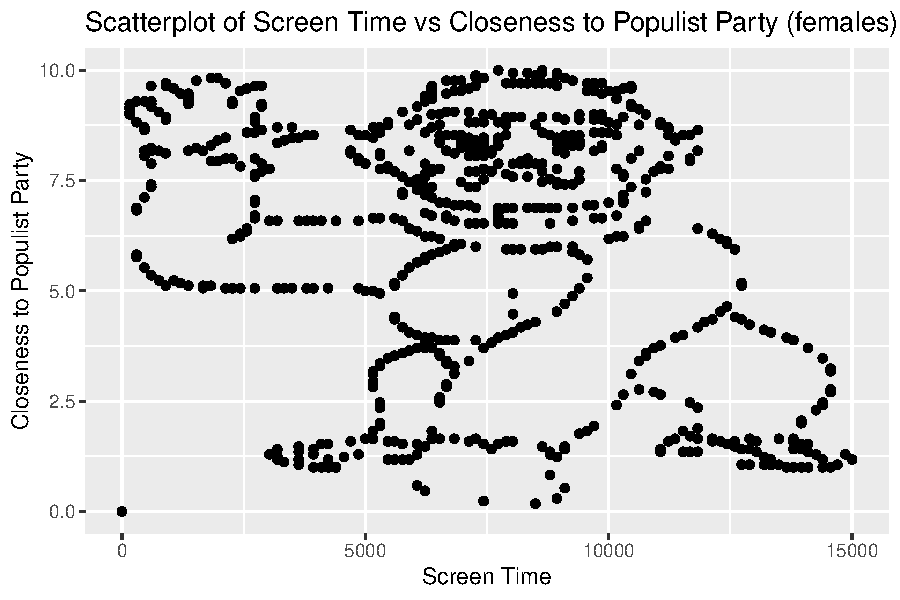
\includegraphics{_main_files/figure-latex/unnamed-chunk-23-1.pdf}

Graph for males here.

\begin{Shaded}
\begin{Highlighting}[]
\FunctionTok{ggplot}\NormalTok{(male, }\FunctionTok{aes}\NormalTok{(}\AttributeTok{x =}\NormalTok{ ScreenTime, }\AttributeTok{y =}\NormalTok{ ClosenessPopulistParty)) }\SpecialCharTok{+}
  \FunctionTok{geom\_point}\NormalTok{() }\SpecialCharTok{+}
  \FunctionTok{labs}\NormalTok{(}\AttributeTok{x =} \StringTok{"Screen Time"}\NormalTok{, }\AttributeTok{y =} \StringTok{"Closeness to Populist Party"}\NormalTok{) }\SpecialCharTok{+}
  \FunctionTok{ggtitle}\NormalTok{(}\StringTok{"Scatterplot of Screen Time vs Closeness to Populist Party (males)"}\NormalTok{)}
\end{Highlighting}
\end{Shaded}

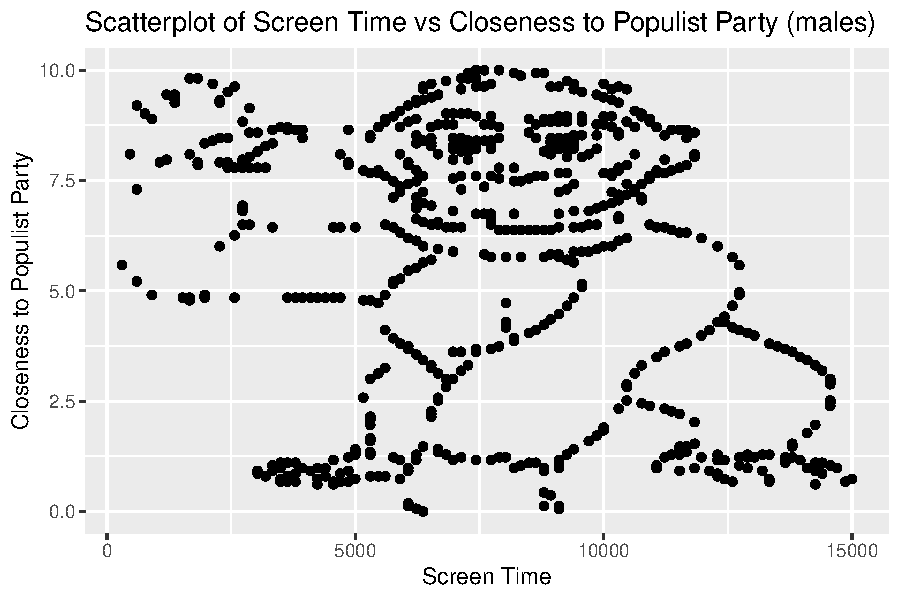
\includegraphics{_main_files/figure-latex/unnamed-chunk-24-1.pdf}

Graph for females and males together here.

\begin{Shaded}
\begin{Highlighting}[]
\FunctionTok{ggplot}\NormalTok{(all\_bindrows, }\FunctionTok{aes}\NormalTok{(}\AttributeTok{x =}\NormalTok{ ScreenTime, }\AttributeTok{y =}\NormalTok{ ClosenessPopulistParty, }\AttributeTok{color =} \FunctionTok{as.factor}\NormalTok{(female))) }\SpecialCharTok{+}
  \FunctionTok{geom\_point}\NormalTok{() }\SpecialCharTok{+}
  \FunctionTok{labs}\NormalTok{(}\AttributeTok{x =} \StringTok{"Screen Time"}\NormalTok{, }\AttributeTok{y =} \StringTok{"Closeness to Populist Party"}\NormalTok{, }\AttributeTok{color =} \StringTok{"Female"}\NormalTok{) }\SpecialCharTok{+}
  \FunctionTok{ggtitle}\NormalTok{(}\StringTok{"Scatterplot of Screen Time vs Closeness to Populist Party by Sex"}\NormalTok{) }\SpecialCharTok{+}
  \FunctionTok{scale\_color\_manual}\NormalTok{(}\AttributeTok{values =} \FunctionTok{c}\NormalTok{(}\StringTok{"1"} \OtherTok{=} \StringTok{"blue"}\NormalTok{, }\StringTok{"0"} \OtherTok{=} \StringTok{"red"}\NormalTok{))  }\CommentTok{\# Define color mapping}
\end{Highlighting}
\end{Shaded}

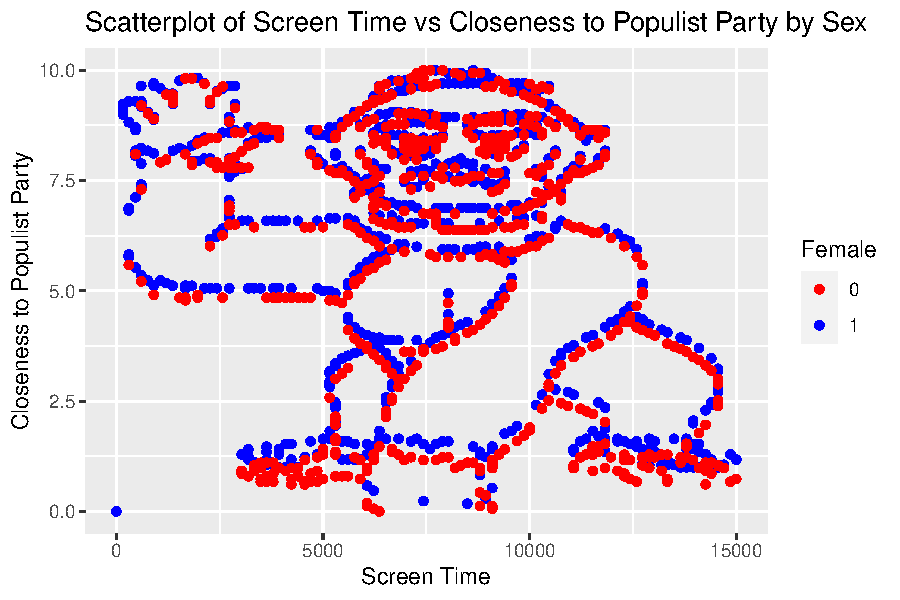
\includegraphics{_main_files/figure-latex/unnamed-chunk-25-1.pdf}

This exercise was a \textbf{cautionary tale} that aims at highlighting the importance to perform preliminary exploratory analysis on your data. What are the gorillas of your data? For example, have you found people with heights of 10 meters? Have you found systematic but unexpected relationships in the data? What are they due to? Mistakes in data management or measurement? To the phenomenon itself? What relations between variables could guide your analysis?

Preliminary analyses include but are not restricted to:

\begin{enumerate}
\def\labelenumi{\roman{enumi}.}
\tightlist
\item
  Generate scatter plots across many variables
\end{enumerate}

\begin{Shaded}
\begin{Highlighting}[]
\FunctionTok{ggpairs}\NormalTok{(all\_bindrows)}
\end{Highlighting}
\end{Shaded}

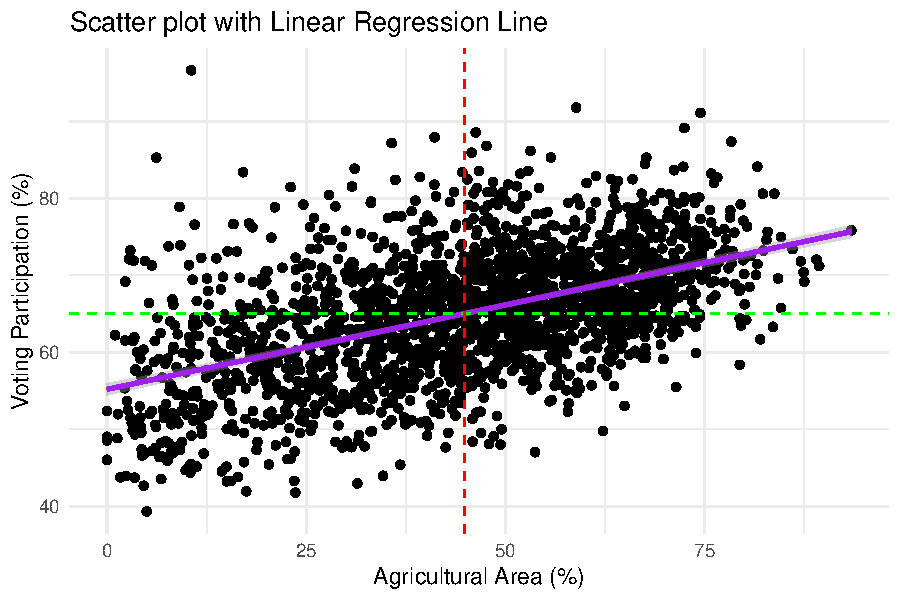
\includegraphics{_main_files/figure-latex/unnamed-chunk-26-1.pdf}

\begin{Shaded}
\begin{Highlighting}[]
\FunctionTok{pairs}\NormalTok{(all\_bindrows)}
\end{Highlighting}
\end{Shaded}

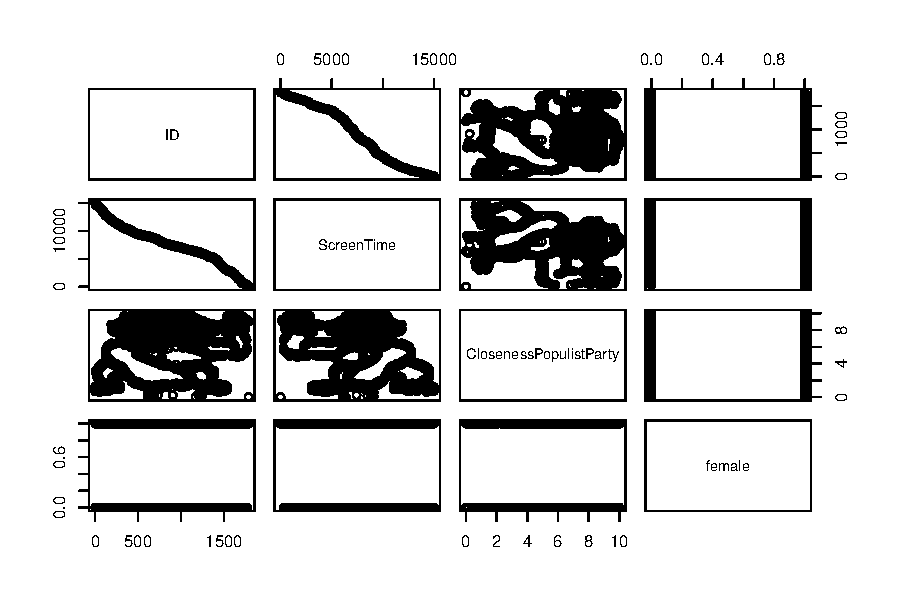
\includegraphics{_main_files/figure-latex/unnamed-chunk-26-2.pdf}
ii. Generate histograms

\begin{Shaded}
\begin{Highlighting}[]
\FunctionTok{ggplot}\NormalTok{(all\_bindrows, }\FunctionTok{aes\_string}\NormalTok{(}\AttributeTok{x =} \StringTok{\textquotesingle{}ScreenTime\textquotesingle{}}\NormalTok{)) }\SpecialCharTok{+} 
      \FunctionTok{geom\_histogram}\NormalTok{(}\AttributeTok{bins =} \DecValTok{30}\NormalTok{, }\AttributeTok{fill =} \StringTok{"blue"}\NormalTok{, }\AttributeTok{color =} \StringTok{"black"}\NormalTok{) }\SpecialCharTok{+}
      \FunctionTok{labs}\NormalTok{(}\AttributeTok{title =} \FunctionTok{paste}\NormalTok{(}\StringTok{"Histogram of"}\NormalTok{, }\StringTok{\textquotesingle{}ScreenTime\textquotesingle{}}\NormalTok{), }\AttributeTok{x =} \StringTok{\textquotesingle{}ScreenTime\textquotesingle{}}\NormalTok{, }\AttributeTok{y =} \StringTok{"Frequency"}\NormalTok{)}
\end{Highlighting}
\end{Shaded}

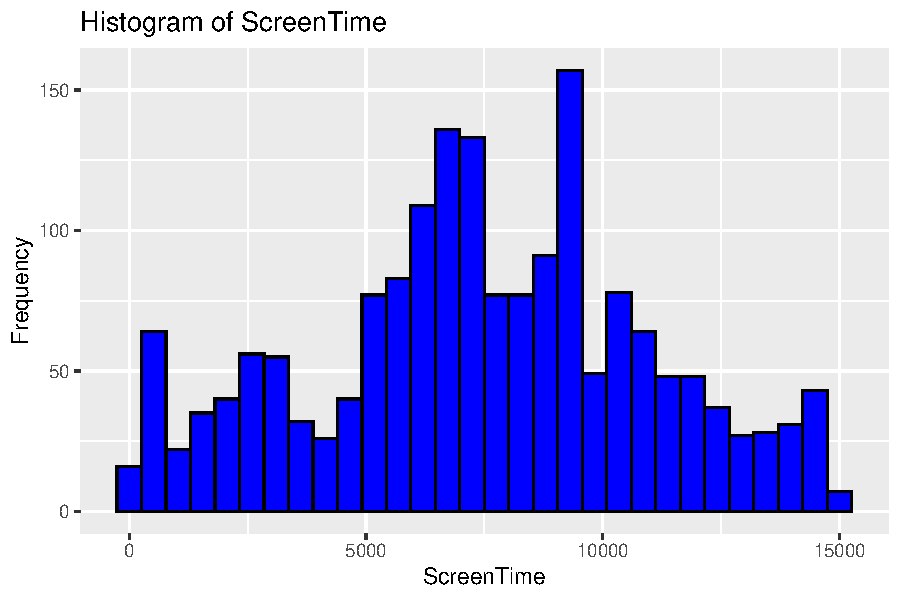
\includegraphics{_main_files/figure-latex/unnamed-chunk-27-1.pdf}

\begin{Shaded}
\begin{Highlighting}[]
\FunctionTok{ggplot}\NormalTok{(all\_bindrows, }\FunctionTok{aes\_string}\NormalTok{(}\AttributeTok{x =} \StringTok{"ClosenessPopulistParty"}\NormalTok{)) }\SpecialCharTok{+} 
      \FunctionTok{geom\_histogram}\NormalTok{(}\AttributeTok{bins =} \DecValTok{30}\NormalTok{, }\AttributeTok{fill =} \StringTok{"blue"}\NormalTok{, }\AttributeTok{color =} \StringTok{"black"}\NormalTok{) }\SpecialCharTok{+}
      \FunctionTok{labs}\NormalTok{(}\AttributeTok{title =} \FunctionTok{paste}\NormalTok{(}\StringTok{"Histogram of"}\NormalTok{, }\StringTok{\textquotesingle{}ClosenessPopulistParty\textquotesingle{}}\NormalTok{), }\AttributeTok{x =} \StringTok{\textquotesingle{}ClosenessPopulistParty\textquotesingle{}}\NormalTok{, }\AttributeTok{y =} \StringTok{"Frequency"}\NormalTok{)}
\end{Highlighting}
\end{Shaded}

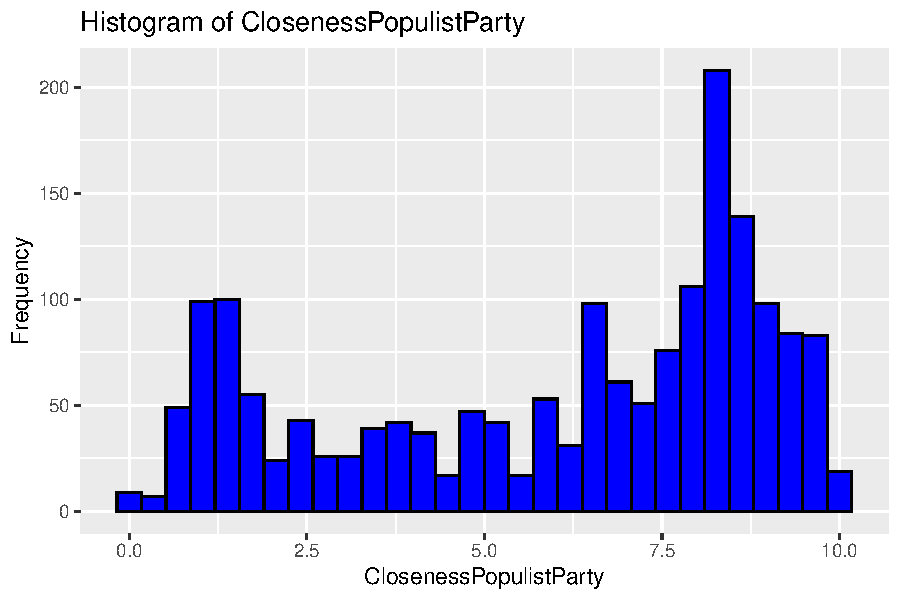
\includegraphics{_main_files/figure-latex/unnamed-chunk-28-1.pdf}

\begin{Shaded}
\begin{Highlighting}[]
\FunctionTok{ggplot}\NormalTok{(all\_bindrows, }\FunctionTok{aes\_string}\NormalTok{(}\AttributeTok{x =} \StringTok{\textquotesingle{}female\textquotesingle{}}\NormalTok{)) }\SpecialCharTok{+} 
      \FunctionTok{geom\_histogram}\NormalTok{(}\AttributeTok{bins =} \DecValTok{30}\NormalTok{, }\AttributeTok{fill =} \StringTok{"blue"}\NormalTok{, }\AttributeTok{color =} \StringTok{"black"}\NormalTok{) }\SpecialCharTok{+}
      \FunctionTok{labs}\NormalTok{(}\AttributeTok{title =} \FunctionTok{paste}\NormalTok{(}\StringTok{"Histogram of"}\NormalTok{, }\StringTok{\textquotesingle{}female\textquotesingle{}}\NormalTok{), }\AttributeTok{x =} \StringTok{\textquotesingle{}female\textquotesingle{}}\NormalTok{, }\AttributeTok{y =} \StringTok{"Frequency"}\NormalTok{)}
\end{Highlighting}
\end{Shaded}

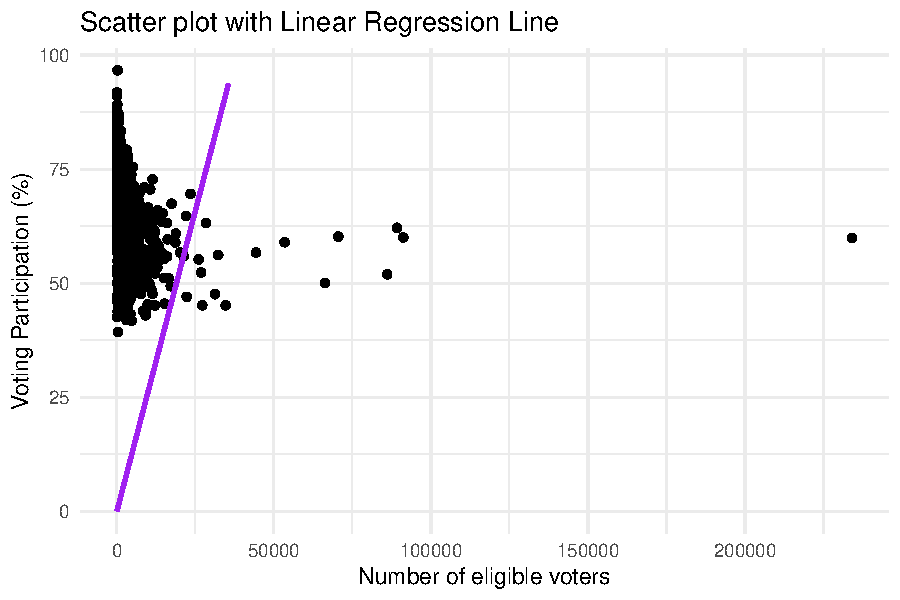
\includegraphics{_main_files/figure-latex/unnamed-chunk-29-1.pdf}

\hypertarget{week-2}{%
\chapter{Week 2}\label{week-2}}

\hypertarget{exercise}{%
\section{Exercise}\label{exercise}}

\begin{itemize}
\tightlist
\item
  2nd: simulated dataset and increase the variance: how does that affects the standard error
\end{itemize}

\hypertarget{solution}{%
\section{Solution}\label{solution}}

\begin{itemize}
\item
  Data taken from \href{https://communities.sas.com/t5/Graphics-Programming/Fun-With-SAS-ODS-Graphics-Don-t-Miss-the-Gorilla-in-the-Data/td-p/697286}{here}.
\item
  Original selective attention, \href{https://www.youtube.com/watch?v=vJG698U2Mvo}{here}.
\item
  Suicide awareness campaign, \href{https://www.youtube.com/watch?v=Lw-YPKR0grk}{here}.
\end{itemize}

\hypertarget{week-3-regression-i-prediction}{%
\chapter{Week 3: Regression I (Prediction)}\label{week-3-regression-i-prediction}}

\hypertarget{aims-1}{%
\section{Aims}\label{aims-1}}

\begin{enumerate}
\def\labelenumi{\arabic{enumi}.}
\tightlist
\item
  Using regression analysis for quantitative descriptive purposes with real data
\item
  Using simulation to instantiate how different properties of the data generating process alter the reliability of regression analysis
\end{enumerate}

\hypertarget{exercise-context-and-question}{%
\section{Exercise: Context and Question}\label{exercise-context-and-question}}

As developed in the following \href{https://de.wikipedia.org/wiki/Eidgen\%C3\%B6ssische_Abstimmung_\%C3\%BCber_die_Totalrevision_des_CO2-Gesetzes\#:~:text=Die\%20Eidgen\%C3\%B6ssische\%20Abstimmung\%20\%C3\%BCber\%20die,von\%2051\%2C59\%20\%25\%20abgelehnt.}{entry}, a referendum took place in 2021 to assess whether Swiss citizens approved or not a bill aimed at reducing greenhouse gas emissions.

The bill was rejected by a narrow margin: 51.6\% of votes went for the ``No'', while 48.4\% for the ``Yes''. In the media, some analysts commented that a marked division or cleavage between rural and urban voters seems to have led to this result. According to their \textbf{narrative}, a specially high rural turn-out seems to underlie such result. As the analyst commented, most urban inhabitants liked the bill while most rural inhabitants disliked it.

Not satisfied with a simple impression, as a political scientist you want to quantitatively qualify your understanding about what happened in that election. Particularly, you want to know:

\begin{enumerate}
\def\labelenumi{\arabic{enumi}.}
\tightlist
\item
  Given that more rural municipalities have smaller populations, was the turn-out higher in municipalities with smaller populations than in bigger ones?
\item
  Was the turn-out higher in more agricultural municipalities than in less agricultural ones?
\end{enumerate}

Thus, to analytically describe the voting results, you will perform some regressions using the following data.

\hypertarget{exercise-solution}{%
\section{Exercise: solution}\label{exercise-solution}}

\textbf{Note:} Remember that you can copy the code from one point to answer another point. Simply make the necessary adjustments.

\hypertarget{real-data}{%
\subsection{Real data}\label{real-data}}

Open the file \texttt{CO2\_land.csv}.

\begin{Shaded}
\begin{Highlighting}[]
\NormalTok{CO2\_land }\OtherTok{\textless{}{-}} \FunctionTok{read.csv}\NormalTok{(}\StringTok{"Data/CO2\_land.csv"}\NormalTok{, }\AttributeTok{header =} \ConstantTok{TRUE}\NormalTok{)}
\end{Highlighting}
\end{Shaded}

\textbf{Note}: in the Appendix you can find how to get the data using APIs of the Swiss Federal Statistical Office.

Using such a file, you embark in doing the following to answer your two questions:

\begin{enumerate}
\def\labelenumi{\roman{enumi}.}
\tightlist
\item
  Since you want to describe the turn-out across municipalities with different population sizes, you initially think of regressing the turn-out on the population size. As you lack the municipal population, you use the number of eligible voters \texttt{anzahlStimmberechtigte} as a proxy. To have a preliminary notion on the relation between \texttt{stimmbeteiligungInProzent} (Turn-out in percent) on \texttt{anzahlStimmberechtigte} (number of eligible voters), generate a scatter plot and add as many straight lines as you want to visually guess which one would be the one that goes closest to each data point. \href{https://ggplot2.tidyverse.org/reference/geom_abline.html}{This} entry could be of help. Remember that a straight line is defined in therms of its slope and intercept parameters. Begin with a slope of zero and an intercept equal to 50. Then, change only one parameter at a time.
\end{enumerate}

\begin{Shaded}
\begin{Highlighting}[]
\NormalTok{guess\_int\_1}\OtherTok{=} \DecValTok{50}
\NormalTok{guess\_slope\_1}\OtherTok{=} \DecValTok{0}
  
\NormalTok{guess\_int\_2}\OtherTok{=} \FunctionTok{mean}\NormalTok{(CO2\_land}\SpecialCharTok{$}\NormalTok{stimmbeteiligungInProzent, }\AttributeTok{na.rm =} \ConstantTok{TRUE}\NormalTok{)}

\NormalTok{guess\_slope\_3}\OtherTok{=}\SpecialCharTok{{-}}\FloatTok{0.01}
  
\NormalTok{guess\_slope\_4}\OtherTok{=}\SpecialCharTok{{-}}\FloatTok{0.0005}
  
\NormalTok{guess\_slope\_5}\OtherTok{=}\SpecialCharTok{{-}}\FloatTok{0.0003}




\FunctionTok{ggplot}\NormalTok{(CO2\_land, }\FunctionTok{aes}\NormalTok{(}\AttributeTok{x =}\NormalTok{ anzahlStimmberechtigte, }\AttributeTok{y =}\NormalTok{ stimmbeteiligungInProzent)) }\SpecialCharTok{+}
  \FunctionTok{geom\_point}\NormalTok{() }\SpecialCharTok{+}
  \FunctionTok{geom\_abline}\NormalTok{(}\AttributeTok{intercept =}\NormalTok{ guess\_int\_1,}
              \AttributeTok{slope =}\NormalTok{ guess\_slope\_1, }\AttributeTok{color =} \StringTok{"\#FF0000"}\NormalTok{, }\AttributeTok{size =} \DecValTok{1}\NormalTok{) }\SpecialCharTok{+} \CommentTok{\#first guess}
  
  \FunctionTok{geom\_abline}\NormalTok{(}\AttributeTok{intercept =}\NormalTok{ guess\_int\_2,   }
              \AttributeTok{slope =}\NormalTok{ guess\_slope\_1, }\AttributeTok{color =} \StringTok{"\#FF4500"}\NormalTok{, }\AttributeTok{size =} \DecValTok{1}\NormalTok{) }\SpecialCharTok{+} \CommentTok{\#a good guess, only changing intercept}
  
  \FunctionTok{geom\_abline}\NormalTok{(}\AttributeTok{intercept =}\NormalTok{ guess\_int\_2, }
              \AttributeTok{slope =}\NormalTok{ guess\_slope\_3, }\AttributeTok{color =} \StringTok{"\#FFA500"}\NormalTok{, }\AttributeTok{size =} \DecValTok{1}\NormalTok{) }\SpecialCharTok{+} \CommentTok{\#decreasing the slope, keeping the intercept}
  
  \FunctionTok{geom\_abline}\NormalTok{(}\AttributeTok{intercept =}\NormalTok{ guess\_int\_2, }
              \AttributeTok{slope =}\NormalTok{ guess\_slope\_4, }\AttributeTok{color =} \StringTok{"\#9ACD32"}\NormalTok{, }\AttributeTok{size =} \DecValTok{1}\NormalTok{) }\SpecialCharTok{+} \CommentTok{\#decreasing the slope, keeping the intercept}
  
  \FunctionTok{geom\_abline}\NormalTok{(}\AttributeTok{intercept =}\NormalTok{ guess\_int\_2,   }
              \AttributeTok{slope =}\NormalTok{ guess\_slope\_5, }\AttributeTok{color =} \StringTok{"\#008000"}\NormalTok{, }\AttributeTok{size =} \DecValTok{1}\NormalTok{) }\SpecialCharTok{+} \CommentTok{\#best visual guess}

  \FunctionTok{scale\_y\_continuous}\NormalTok{(}\AttributeTok{limits =} \FunctionTok{c}\NormalTok{(}\DecValTok{0}\NormalTok{, }\FunctionTok{max}\NormalTok{(CO2\_land}\SpecialCharTok{$}\NormalTok{stimmbeteiligungInProzent, }\AttributeTok{na.rm =} \ConstantTok{TRUE}\NormalTok{))) }\SpecialCharTok{+}  
  \FunctionTok{theme\_minimal}\NormalTok{() }\SpecialCharTok{+}
  \FunctionTok{theme}\NormalTok{(}\AttributeTok{plot.title =} \FunctionTok{element\_text}\NormalTok{(}\AttributeTok{hjust =} \FloatTok{0.5}\NormalTok{)) }\SpecialCharTok{+}

  \FunctionTok{labs}\NormalTok{(}
    \AttributeTok{x =} \StringTok{"Number of eligible voters"}\NormalTok{,}
    \AttributeTok{y =} \StringTok{"Turn{-}out (\%)"}\NormalTok{,}
    \AttributeTok{title =} \StringTok{"Scatter plot with straight lines using the eye{-}meter"}
\NormalTok{  )}
\end{Highlighting}
\end{Shaded}

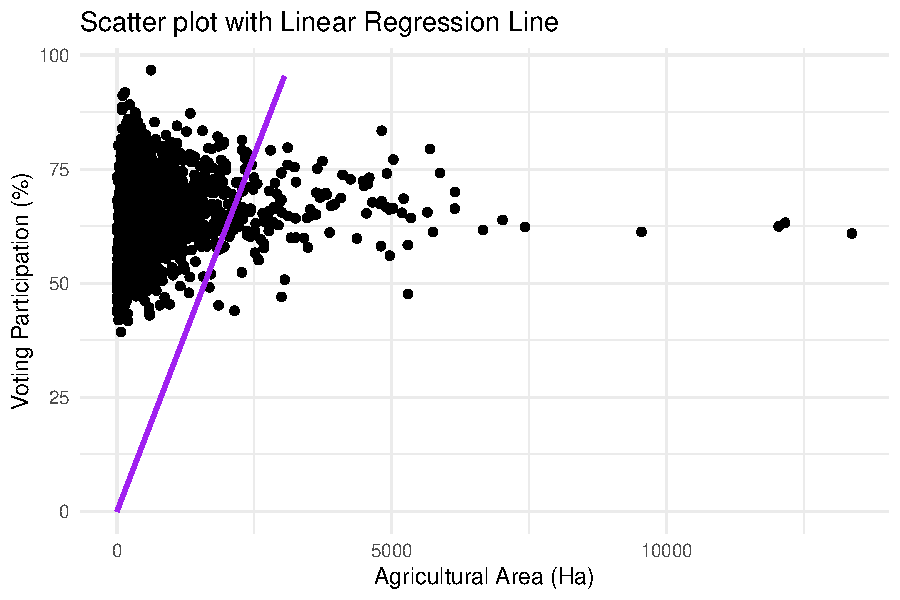
\includegraphics{_main_files/figure-latex/unnamed-chunk-32-1.pdf}

\begin{enumerate}
\def\labelenumi{\roman{enumi}.}
\setcounter{enumi}{1}
\tightlist
\item
  Add to the previous graph the linear regression line.
\end{enumerate}

\begin{Shaded}
\begin{Highlighting}[]
\FunctionTok{ggplot}\NormalTok{(CO2\_land, }\FunctionTok{aes}\NormalTok{(}\AttributeTok{x =}\NormalTok{ anzahlStimmberechtigte, }\AttributeTok{y =}\NormalTok{ stimmbeteiligungInProzent)) }\SpecialCharTok{+}
  \FunctionTok{geom\_point}\NormalTok{() }\SpecialCharTok{+}
  \FunctionTok{geom\_abline}\NormalTok{(}\AttributeTok{intercept =}\NormalTok{ guess\_int\_1,}
              \AttributeTok{slope =}\NormalTok{ guess\_slope\_1, }\AttributeTok{color =} \StringTok{"\#FF0000"}\NormalTok{, }\AttributeTok{size =} \DecValTok{1}\NormalTok{) }\SpecialCharTok{+} \CommentTok{\#first guess}
  
  \FunctionTok{geom\_abline}\NormalTok{(}\AttributeTok{intercept =}\NormalTok{ guess\_int\_2,   }
              \AttributeTok{slope =}\NormalTok{ guess\_slope\_1, }\AttributeTok{color =} \StringTok{"\#FF4500"}\NormalTok{, }\AttributeTok{size =} \DecValTok{1}\NormalTok{) }\SpecialCharTok{+} \CommentTok{\#a good guess, only changing intercept}
  
  \FunctionTok{geom\_abline}\NormalTok{(}\AttributeTok{intercept =}\NormalTok{ guess\_int\_2, }
              \AttributeTok{slope =}\NormalTok{ guess\_slope\_3, }\AttributeTok{color =} \StringTok{"\#FFA500"}\NormalTok{, }\AttributeTok{size =} \DecValTok{1}\NormalTok{) }\SpecialCharTok{+} \CommentTok{\#decreasing the slope, keeping the intercept}
  
  \FunctionTok{geom\_abline}\NormalTok{(}\AttributeTok{intercept =}\NormalTok{ guess\_int\_2, }
              \AttributeTok{slope =}\NormalTok{ guess\_slope\_4, }\AttributeTok{color =} \StringTok{"\#9ACD32"}\NormalTok{, }\AttributeTok{size =} \DecValTok{1}\NormalTok{) }\SpecialCharTok{+} \CommentTok{\#decreasing the slope, keeping the intercept}
  
  \FunctionTok{geom\_abline}\NormalTok{(}\AttributeTok{intercept =}\NormalTok{ guess\_int\_2,   }
              \AttributeTok{slope =}\NormalTok{ guess\_slope\_5, }\AttributeTok{color =} \StringTok{"\#008000"}\NormalTok{, }\AttributeTok{size =} \DecValTok{1}\NormalTok{) }\SpecialCharTok{+} \CommentTok{\#best visual guess}
  
  \FunctionTok{geom\_smooth}\NormalTok{(}\AttributeTok{method =} \StringTok{"lm"}\NormalTok{, }\AttributeTok{formula =}\NormalTok{ y }\SpecialCharTok{\textasciitilde{}}\NormalTok{ x, }\AttributeTok{se =} \ConstantTok{FALSE}\NormalTok{, }\AttributeTok{color =} \StringTok{"green"}\NormalTok{) }\SpecialCharTok{+}  \CommentTok{\#mathematically estimated best possible parameters}
  \FunctionTok{scale\_y\_continuous}\NormalTok{(}\AttributeTok{limits =} \FunctionTok{c}\NormalTok{(}\DecValTok{0}\NormalTok{, }\FunctionTok{max}\NormalTok{(CO2\_land}\SpecialCharTok{$}\NormalTok{stimmbeteiligungInProzent, }\AttributeTok{na.rm =} \ConstantTok{TRUE}\NormalTok{))) }\SpecialCharTok{+}  
  \FunctionTok{theme\_minimal}\NormalTok{() }\SpecialCharTok{+}
  \FunctionTok{theme}\NormalTok{(}\AttributeTok{plot.title =} \FunctionTok{element\_text}\NormalTok{(}\AttributeTok{hjust =} \FloatTok{0.5}\NormalTok{)) }\SpecialCharTok{+}

  \FunctionTok{labs}\NormalTok{(}
    \AttributeTok{x =} \StringTok{"Number of eligible voters"}\NormalTok{,}
    \AttributeTok{y =} \StringTok{"Turn{-}out (\%)"}\NormalTok{,}
    \AttributeTok{title =} \StringTok{"Scatter plot with straight lines using the eye{-}meter and the regression line"}
\NormalTok{  )}
\end{Highlighting}
\end{Shaded}

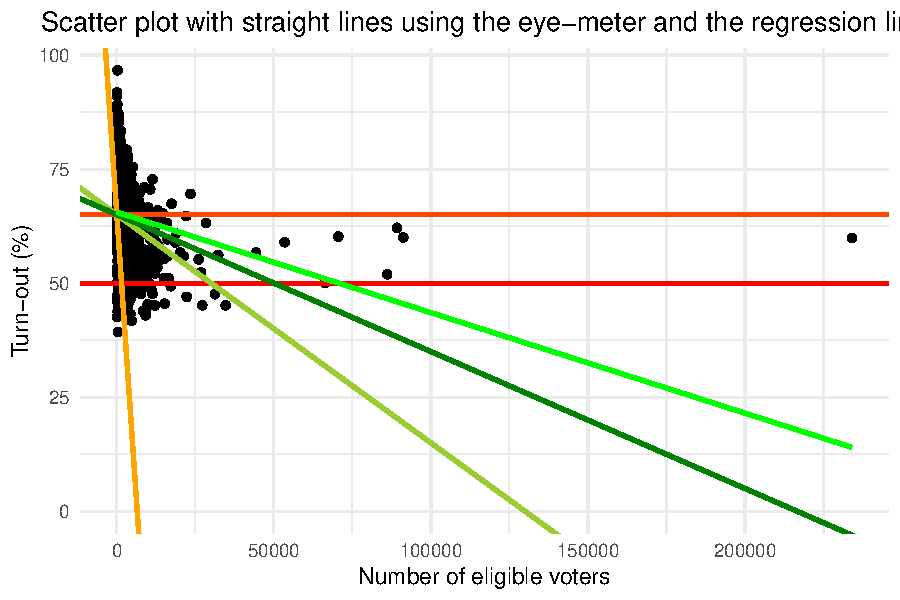
\includegraphics{_main_files/figure-latex/unnamed-chunk-33-1.pdf}

\begin{enumerate}
\def\labelenumi{\roman{enumi}.}
\setcounter{enumi}{2}
\tightlist
\item
  You have now instantiated the intuition behind the linear regression by forming different lines that are visually intuitive about the relation between our variables of interest. Since you know that the linear regression line is the straight line that is closest to all points, you want to go beyond your ``eye-meter'' and use a precise measurement. Regress \texttt{stimmbeteiligungInProzent} on \texttt{anzahlStimmberechtigte}. Report and interpret the parameters.
\end{enumerate}

Write the regression here.

\begin{Shaded}
\begin{Highlighting}[]
\NormalTok{result1 }\OtherTok{\textless{}{-}} \FunctionTok{lm}\NormalTok{(stimmbeteiligungInProzent }\SpecialCharTok{\textasciitilde{}}\NormalTok{ anzahlStimmberechtigte , }\AttributeTok{data =}\NormalTok{ CO2\_land)}
\FunctionTok{summary}\NormalTok{(result1)}
\end{Highlighting}
\end{Shaded}

\begin{verbatim}
## 
## Call:
## lm(formula = stimmbeteiligungInProzent ~ anzahlStimmberechtigte, 
##     data = CO2_land)
## 
## Residuals:
##     Min      1Q  Median      3Q     Max 
## -26.173  -5.185   0.244   5.365  45.871 
## 
## Coefficients:
##                          Estimate Std. Error t value Pr(>|t|)    
## (Intercept)             6.558e+01  1.832e-01 358.048   <2e-16 ***
## anzahlStimmberechtigte -2.202e-04  2.408e-05  -9.146   <2e-16 ***
## ---
## Signif. codes:  0 '***' 0.001 '**' 0.01 '*' 0.05 '.' 0.1 ' ' 1
## 
## Residual standard error: 7.98 on 2130 degrees of freedom
## Multiple R-squared:  0.03779,    Adjusted R-squared:  0.03734 
## F-statistic: 83.65 on 1 and 2130 DF,  p-value: < 2.2e-16
\end{verbatim}

Report and interpret the parameters here:

\begin{Shaded}
\begin{Highlighting}[]
\NormalTok{coeffs1}\OtherTok{\textless{}{-}} \FunctionTok{coef}\NormalTok{(result1)}
\NormalTok{coeffs1}
\end{Highlighting}
\end{Shaded}

\begin{verbatim}
##            (Intercept) anzahlStimmberechtigte 
##          65.5802858731          -0.0002202479
\end{verbatim}

The estimated (Intercept) is 65.58, while the estimated slope for anzahlStimmberechtigte is \ensuremath{-2.2\times 10^{-4}}. It means that, across Swiss municipalities, an increase of a thousand voters was associated with an average decrease in the turn-out of -0.22 percentage points.

\begin{enumerate}
\def\labelenumi{\roman{enumi}.}
\setcounter{enumi}{3}
\tightlist
\item
  Since you don't want to take for granted that the mathematically estimated parameters are the ones that generate the best possible fit for a straight line, you want to compare the Sum of Squared Residuals (SSR) across the lines that you generated in the previous point. Generate and compare the SSR for each of those lines. Are the parameters estimated by R the best among your estimations?
\end{enumerate}

\begin{Shaded}
\begin{Highlighting}[]
\CommentTok{\# It\textquotesingle{}s easier to calculate the residuals simply using the model}
\NormalTok{CO2\_land}\SpecialCharTok{$}\NormalTok{ResidRegression}\OtherTok{\textless{}{-}} \FunctionTok{residuals}\NormalTok{(result1)}
\NormalTok{CO2\_land}\SpecialCharTok{$}\NormalTok{SqResidRegression}\OtherTok{\textless{}{-}}\NormalTok{ (}\FunctionTok{residuals}\NormalTok{(result1))}\SpecialCharTok{\^{}}\DecValTok{2}
\NormalTok{CO2\_land}\SpecialCharTok{$}\NormalTok{SumSqResidRegression}\OtherTok{\textless{}{-}} \FunctionTok{sum}\NormalTok{(CO2\_land}\SpecialCharTok{$}\NormalTok{SqResidRegression)}

\CommentTok{\#But it\textquotesingle{}s also possible to easily calculate the squared residuals (SR) for each model}

\NormalTok{CO2\_land}\SpecialCharTok{$}\NormalTok{SR\_Guess1}\OtherTok{=}\NormalTok{ ((guess\_int\_1 }\SpecialCharTok{+}\NormalTok{ guess\_slope\_1 }\SpecialCharTok{*}\NormalTok{ CO2\_land}\SpecialCharTok{$}\NormalTok{anzahlStimmberechtigte)}\SpecialCharTok{{-}}\NormalTok{CO2\_land}\SpecialCharTok{$}\NormalTok{stimmbeteiligungInProzent)}\SpecialCharTok{\^{}}\DecValTok{2}
\NormalTok{CO2\_land}\SpecialCharTok{$}\NormalTok{SR\_Guess2}\OtherTok{=}\NormalTok{ ((guess\_int\_2 }\SpecialCharTok{+}\NormalTok{ guess\_slope\_1 }\SpecialCharTok{*}\NormalTok{ CO2\_land}\SpecialCharTok{$}\NormalTok{anzahlStimmberechtigte)}\SpecialCharTok{{-}}\NormalTok{CO2\_land}\SpecialCharTok{$}\NormalTok{stimmbeteiligungInProzent)}\SpecialCharTok{\^{}}\DecValTok{2}
\NormalTok{CO2\_land}\SpecialCharTok{$}\NormalTok{SR\_Guess3}\OtherTok{=}\NormalTok{ ((guess\_int\_1 }\SpecialCharTok{+}\NormalTok{ guess\_slope\_3 }\SpecialCharTok{*}\NormalTok{ CO2\_land}\SpecialCharTok{$}\NormalTok{anzahlStimmberechtigte)}\SpecialCharTok{{-}}\NormalTok{CO2\_land}\SpecialCharTok{$}\NormalTok{stimmbeteiligungInProzent)}\SpecialCharTok{\^{}}\DecValTok{2}
\NormalTok{CO2\_land}\SpecialCharTok{$}\NormalTok{SR\_Guess4}\OtherTok{=}\NormalTok{ ((guess\_int\_1 }\SpecialCharTok{+}\NormalTok{ guess\_slope\_4 }\SpecialCharTok{*}\NormalTok{ CO2\_land}\SpecialCharTok{$}\NormalTok{anzahlStimmberechtigte)}\SpecialCharTok{{-}}\NormalTok{CO2\_land}\SpecialCharTok{$}\NormalTok{stimmbeteiligungInProzent)}\SpecialCharTok{\^{}}\DecValTok{2}
\NormalTok{CO2\_land}\SpecialCharTok{$}\NormalTok{SR\_Guess5}\OtherTok{=}\NormalTok{ ((guess\_int\_1 }\SpecialCharTok{+}\NormalTok{ guess\_slope\_5 }\SpecialCharTok{*}\NormalTok{ CO2\_land}\SpecialCharTok{$}\NormalTok{anzahlStimmberechtigte)}\SpecialCharTok{{-}}\NormalTok{CO2\_land}\SpecialCharTok{$}\NormalTok{stimmbeteiligungInProzent)}\SpecialCharTok{\^{}}\DecValTok{2}

\CommentTok{\# And sum of squared residuals (SSR)}
\NormalTok{CO2\_land}\SpecialCharTok{$}\NormalTok{SSR\_Guess1}\OtherTok{=} \FunctionTok{sum}\NormalTok{(CO2\_land}\SpecialCharTok{$}\NormalTok{SR\_Guess1)}
\NormalTok{CO2\_land}\SpecialCharTok{$}\NormalTok{SSR\_Guess2}\OtherTok{=} \FunctionTok{sum}\NormalTok{(CO2\_land}\SpecialCharTok{$}\NormalTok{SR\_Guess2)}
\NormalTok{CO2\_land}\SpecialCharTok{$}\NormalTok{SSR\_Guess3}\OtherTok{=} \FunctionTok{sum}\NormalTok{(CO2\_land}\SpecialCharTok{$}\NormalTok{SR\_Guess3)}
\NormalTok{CO2\_land}\SpecialCharTok{$}\NormalTok{SSR\_Guess4}\OtherTok{=} \FunctionTok{sum}\NormalTok{(CO2\_land}\SpecialCharTok{$}\NormalTok{SR\_Guess4)}
\NormalTok{CO2\_land}\SpecialCharTok{$}\NormalTok{SSR\_Guess5}\OtherTok{=} \FunctionTok{sum}\NormalTok{(CO2\_land}\SpecialCharTok{$}\NormalTok{SR\_Guess5)}

\ControlFlowTok{if}\NormalTok{ ((CO2\_land}\SpecialCharTok{$}\NormalTok{SumSqResidRegression[}\DecValTok{1}\NormalTok{]}\SpecialCharTok{\textless{}}\NormalTok{CO2\_land}\SpecialCharTok{$}\NormalTok{SSR\_Guess1[}\DecValTok{1}\NormalTok{]) }\SpecialCharTok{\&}\NormalTok{ (CO2\_land}\SpecialCharTok{$}\NormalTok{SumSqResidRegression[}\DecValTok{1}\NormalTok{]}\SpecialCharTok{\textless{}}\NormalTok{CO2\_land}\SpecialCharTok{$}\NormalTok{SSR\_Guess2[}\DecValTok{1}\NormalTok{]) }\SpecialCharTok{\&}\NormalTok{ (CO2\_land}\SpecialCharTok{$}\NormalTok{SumSqResidRegression[}\DecValTok{1}\NormalTok{]}\SpecialCharTok{\textless{}}\NormalTok{CO2\_land}\SpecialCharTok{$}\NormalTok{SSR\_Guess3[}\DecValTok{1}\NormalTok{]) }\SpecialCharTok{\&}\NormalTok{ (CO2\_land}\SpecialCharTok{$}\NormalTok{SumSqResidRegression[}\DecValTok{1}\NormalTok{]}\SpecialCharTok{\textless{}}\NormalTok{CO2\_land}\SpecialCharTok{$}\NormalTok{SSR\_Guess4[}\DecValTok{1}\NormalTok{]) }\SpecialCharTok{\&}\NormalTok{ (CO2\_land}\SpecialCharTok{$}\NormalTok{SumSqResidRegression[}\DecValTok{1}\NormalTok{]}\SpecialCharTok{\textless{}}\NormalTok{CO2\_land}\SpecialCharTok{$}\NormalTok{SSR\_Guess5[}\DecValTok{1}\NormalTok{]))\{}
  \FunctionTok{print}\NormalTok{(}\StringTok{"Yes, as it is mathematically necessary, the SSR for the mathematically estimated model is the lowest across all estimated scenarios! :)"}\NormalTok{)}
\NormalTok{\}}
\end{Highlighting}
\end{Shaded}

\begin{verbatim}
## [1] "Yes, as it is mathematically necessary, the SSR for the mathematically estimated model is the lowest across all estimated scenarios! :)"
\end{verbatim}

\begin{enumerate}
\def\labelenumi{\alph{enumi}.}
\setcounter{enumi}{21}
\tightlist
\item
  Notice that some few municipalities have numbers of voters that are very high compared to the typical values. As a consequence, the regression line is very influenced by those observations (i.e., small displacements in the area where there are many observations have a lower influence on the line than displacements of the same magnitude and direction in the area with few observations). As a consequence, you want to analyze how do the previous estimates change when you restrict your analysis to municipalities with less than 50K eligible voters. Estimate the regression and compare the respective parameters of the models. What slope is higher? What intercept is higher? How does obviating those observations influence our parameters?
\end{enumerate}

\begin{Shaded}
\begin{Highlighting}[]
\NormalTok{CO2\_land\_filtered }\OtherTok{\textless{}{-}}\NormalTok{ CO2\_land }\SpecialCharTok{\%\textgreater{}\%} 
  \FunctionTok{filter}\NormalTok{(anzahlStimmberechtigte }\SpecialCharTok{\textless{}} \DecValTok{50000}\NormalTok{)}

\NormalTok{result2 }\OtherTok{\textless{}{-}} \FunctionTok{lm}\NormalTok{(stimmbeteiligungInProzent }\SpecialCharTok{\textasciitilde{}}\NormalTok{ anzahlStimmberechtigte , }\AttributeTok{data =}\NormalTok{ CO2\_land\_filtered)}
\FunctionTok{summary}\NormalTok{(result2)}
\end{Highlighting}
\end{Shaded}

\begin{verbatim}
## 
## Call:
## lm(formula = stimmbeteiligungInProzent ~ anzahlStimmberechtigte, 
##     data = CO2_land_filtered)
## 
## Residuals:
##      Min       1Q   Median       3Q      Max 
## -27.3197  -4.6709   0.2374   4.9221  29.8830 
## 
## Coefficients:
##                          Estimate Std. Error t value Pr(>|t|)    
## (Intercept)             6.698e+01  1.997e-01   335.3   <2e-16 ***
## anzahlStimmberechtigte -8.762e-04  5.093e-05   -17.2   <2e-16 ***
## ---
## Signif. codes:  0 '***' 0.001 '**' 0.01 '*' 0.05 '.' 0.1 ' ' 1
## 
## Residual standard error: 7.62 on 2123 degrees of freedom
## Multiple R-squared:  0.1224, Adjusted R-squared:  0.122 
## F-statistic:   296 on 1 and 2123 DF,  p-value: < 2.2e-16
\end{verbatim}

\begin{Shaded}
\begin{Highlighting}[]
\NormalTok{coeffs2}\OtherTok{\textless{}{-}} \FunctionTok{coef}\NormalTok{(result2)}
\NormalTok{coeffs2}
\end{Highlighting}
\end{Shaded}

\begin{verbatim}
##            (Intercept) anzahlStimmberechtigte 
##          66.9791169423          -0.0008762278
\end{verbatim}

\begin{Shaded}
\begin{Highlighting}[]
\ControlFlowTok{if}\NormalTok{ ((coeffs1[}\DecValTok{1}\NormalTok{]}\SpecialCharTok{\textgreater{}}\NormalTok{coeffs2[}\DecValTok{1}\NormalTok{]) }\SpecialCharTok{\&}\NormalTok{ (coeffs1[}\DecValTok{1}\NormalTok{]}\SpecialCharTok{!=}\NormalTok{coeffs2[}\DecValTok{1}\NormalTok{]))\{}
  \FunctionTok{print}\NormalTok{(}\StringTok{"The original model has a higher intercept than the one only on the restricted observations."}\NormalTok{)}
\NormalTok{\} }\ControlFlowTok{else}\NormalTok{\{}
  \FunctionTok{print}\NormalTok{(}\StringTok{"The model only on the restricted observations has a higher intercept than the original one."}\NormalTok{)}
\NormalTok{\}}
\end{Highlighting}
\end{Shaded}

\begin{verbatim}
## [1] "The model only on the restricted observations has a higher intercept than the original one."
\end{verbatim}

\begin{Shaded}
\begin{Highlighting}[]
\ControlFlowTok{if}\NormalTok{ ((coeffs1[}\DecValTok{2}\NormalTok{]}\SpecialCharTok{\textgreater{}}\NormalTok{coeffs2[}\DecValTok{2}\NormalTok{]) }\SpecialCharTok{\&}\NormalTok{ (coeffs1[}\DecValTok{2}\NormalTok{]}\SpecialCharTok{!=}\NormalTok{coeffs2[}\DecValTok{2}\NormalTok{]))\{}
  \FunctionTok{print}\NormalTok{(}\StringTok{"The original model has a higher slope than the one only on the restricted observations."}\NormalTok{)}
\NormalTok{\} }\ControlFlowTok{else}\NormalTok{\{}
  \FunctionTok{print}\NormalTok{(}\StringTok{"The model only on the restricted observations has a higher slope than the original one."}\NormalTok{)}
\NormalTok{\}}
\end{Highlighting}
\end{Shaded}

\begin{verbatim}
## [1] "The original model has a higher slope than the one only on the restricted observations."
\end{verbatim}

The reason the parameters changed is because the new model needs to fit data that is concentrated in a more clearly negative relation between our variables of interest.

\begin{enumerate}
\def\labelenumi{\roman{enumi}.}
\setcounter{enumi}{5}
\item
  {[}Optional{]} Modify slightly the parameters estimated using the linear regression. For example, keeping the intercept unchanged, increase or decrease the slope in 1 percent every time. Now, compare the sum of squared residuals. Do your experiments show smaller SSR? Is it possible?
\item
  Finally, you want to analyze a counterfactual scenario: What would have been the outcome of the referendum should the turn-out in each of the municipalities would have been as high as in Zurich?
\end{enumerate}

\begin{Shaded}
\begin{Highlighting}[]
\NormalTok{OriginalOutcome }\OtherTok{=}  \FunctionTok{sum}\NormalTok{(CO2\_land}\SpecialCharTok{$}\NormalTok{jaStimmenAbsolut)}\SpecialCharTok{/}\NormalTok{(}\FunctionTok{sum}\NormalTok{(CO2\_land}\SpecialCharTok{$}\NormalTok{jaStimmenAbsolut)}\SpecialCharTok{+}\FunctionTok{sum}\NormalTok{(CO2\_land}\SpecialCharTok{$}\NormalTok{neinStimmenAbsolut))}
\NormalTok{CO2\_land}\SpecialCharTok{$}\NormalTok{Valid\_TurnOut }\OtherTok{=}\NormalTok{CO2\_land}\SpecialCharTok{$}\NormalTok{gueltigeStimmen}\SpecialCharTok{/}\NormalTok{CO2\_land}\SpecialCharTok{$}\NormalTok{anzahlStimmberechtigte}

\NormalTok{CO2\_land}\SpecialCharTok{$}\NormalTok{OriginalOutcome\_test }\OtherTok{=}\NormalTok{  CO2\_land}\SpecialCharTok{$}\NormalTok{jaStimmenInProzent }\SpecialCharTok{*}\NormalTok{ CO2\_land}\SpecialCharTok{$}\NormalTok{anzahlStimmberechtigte }\SpecialCharTok{*}\NormalTok{ CO2\_land}\SpecialCharTok{$}\NormalTok{Valid\_TurnOut }\SpecialCharTok{/}\DecValTok{100}



\CommentTok{\# Min}
\NormalTok{TurnOut\_min}\OtherTok{=} \FunctionTok{min}\NormalTok{(CO2\_land}\SpecialCharTok{$}\NormalTok{Valid\_TurnOut)}
\NormalTok{CO2\_land}\SpecialCharTok{$}\NormalTok{Yes\_Conterfactual\_min}\OtherTok{=}\NormalTok{ CO2\_land}\SpecialCharTok{$}\NormalTok{jaStimmenInProzent }\SpecialCharTok{*}\NormalTok{ CO2\_land}\SpecialCharTok{$}\NormalTok{anzahlStimmberechtigte }\SpecialCharTok{*}\NormalTok{ TurnOut\_min }\SpecialCharTok{/}\DecValTok{100}
\NormalTok{CO2\_land}\SpecialCharTok{$}\NormalTok{No\_Conterfactual\_min}\OtherTok{=}\NormalTok{  (}\DecValTok{100}\SpecialCharTok{{-}}\NormalTok{CO2\_land}\SpecialCharTok{$}\NormalTok{jaStimmenInProzent) }\SpecialCharTok{*}\NormalTok{ CO2\_land}\SpecialCharTok{$}\NormalTok{anzahlStimmberechtigte }\SpecialCharTok{*}\NormalTok{ TurnOut\_min }\SpecialCharTok{/}\DecValTok{100}
\NormalTok{CounterfactualOutcome\_min}\OtherTok{=}  \FunctionTok{sum}\NormalTok{(CO2\_land}\SpecialCharTok{$}\NormalTok{Yes\_Conterfactual\_min)}\SpecialCharTok{/}\NormalTok{(}\FunctionTok{sum}\NormalTok{(CO2\_land}\SpecialCharTok{$}\NormalTok{Yes\_Conterfactual\_min)}\SpecialCharTok{+}\FunctionTok{sum}\NormalTok{(CO2\_land}\SpecialCharTok{$}\NormalTok{No\_Conterfactual\_min))}

\CommentTok{\# Max}
\NormalTok{TurnOut\_max}\OtherTok{=} \FunctionTok{max}\NormalTok{(CO2\_land}\SpecialCharTok{$}\NormalTok{Valid\_TurnOut)}
\NormalTok{CO2\_land}\SpecialCharTok{$}\NormalTok{Yes\_Conterfactual\_max}\OtherTok{=}\NormalTok{ CO2\_land}\SpecialCharTok{$}\NormalTok{jaStimmenInProzent }\SpecialCharTok{*}\NormalTok{ CO2\_land}\SpecialCharTok{$}\NormalTok{anzahlStimmberechtigte }\SpecialCharTok{*}\NormalTok{ TurnOut\_max }
\NormalTok{CO2\_land}\SpecialCharTok{$}\NormalTok{No\_Conterfactual\_max}\OtherTok{=}\NormalTok{  (}\DecValTok{100}\SpecialCharTok{{-}}\NormalTok{CO2\_land}\SpecialCharTok{$}\NormalTok{jaStimmenInProzent) }\SpecialCharTok{*}\NormalTok{ CO2\_land}\SpecialCharTok{$}\NormalTok{anzahlStimmberechtigte }\SpecialCharTok{*}\NormalTok{ TurnOut\_max }
\NormalTok{CounterfactualOutcome\_max}\OtherTok{=}  \FunctionTok{sum}\NormalTok{(CO2\_land}\SpecialCharTok{$}\NormalTok{Yes\_Conterfactual\_max)}\SpecialCharTok{/}\NormalTok{(}\FunctionTok{sum}\NormalTok{(CO2\_land}\SpecialCharTok{$}\NormalTok{Yes\_Conterfactual\_max)}\SpecialCharTok{+}\FunctionTok{sum}\NormalTok{(CO2\_land}\SpecialCharTok{$}\NormalTok{No\_Conterfactual\_max))}

\CommentTok{\# Zurich}
\NormalTok{TurnOut\_Zurich}\OtherTok{=}\NormalTok{ CO2\_land}\SpecialCharTok{$}\NormalTok{Valid\_TurnOut[CO2\_land}\SpecialCharTok{$}\NormalTok{mun\_id}\SpecialCharTok{==}\DecValTok{261}\NormalTok{]}
\NormalTok{CO2\_land}\SpecialCharTok{$}\NormalTok{Yes\_Conterfactual\_Zurich}\OtherTok{=}\NormalTok{ CO2\_land}\SpecialCharTok{$}\NormalTok{jaStimmenInProzent }\SpecialCharTok{*}\NormalTok{ CO2\_land}\SpecialCharTok{$}\NormalTok{anzahlStimmberechtigte }\SpecialCharTok{*}\NormalTok{ TurnOut\_Zurich }
\NormalTok{CO2\_land}\SpecialCharTok{$}\NormalTok{No\_Conterfactual\_Zurich}\OtherTok{=}\NormalTok{  (}\DecValTok{100}\SpecialCharTok{{-}}\NormalTok{CO2\_land}\SpecialCharTok{$}\NormalTok{jaStimmenInProzent) }\SpecialCharTok{*}\NormalTok{ CO2\_land}\SpecialCharTok{$}\NormalTok{anzahlStimmberechtigte }\SpecialCharTok{*}\NormalTok{ TurnOut\_Zurich }
\NormalTok{CounterfactualOutcome\_Zurich}\OtherTok{=}  \FunctionTok{sum}\NormalTok{(CO2\_land}\SpecialCharTok{$}\NormalTok{Yes\_Conterfactual\_Zurich)}\SpecialCharTok{/}\NormalTok{(}\FunctionTok{sum}\NormalTok{(CO2\_land}\SpecialCharTok{$}\NormalTok{Yes\_Conterfactual\_Zurich)}\SpecialCharTok{+}\FunctionTok{sum}\NormalTok{(CO2\_land}\SpecialCharTok{$}\NormalTok{No\_Conterfactual\_Zurich))}

\CommentTok{\# Luzern}
\NormalTok{TurnOut\_Luzern}\OtherTok{=}\NormalTok{ CO2\_land}\SpecialCharTok{$}\NormalTok{Valid\_TurnOut[CO2\_land}\SpecialCharTok{$}\NormalTok{mun\_id}\SpecialCharTok{==}\DecValTok{1061}\NormalTok{]}
\NormalTok{CO2\_land}\SpecialCharTok{$}\NormalTok{Yes\_Conterfactual\_Luzern}\OtherTok{=}\NormalTok{ CO2\_land}\SpecialCharTok{$}\NormalTok{jaStimmenInProzent }\SpecialCharTok{*}\NormalTok{ CO2\_land}\SpecialCharTok{$}\NormalTok{anzahlStimmberechtigte }\SpecialCharTok{*}\NormalTok{ TurnOut\_Luzern }
\NormalTok{CO2\_land}\SpecialCharTok{$}\NormalTok{No\_Conterfactual\_Luzern}\OtherTok{=}\NormalTok{  (}\DecValTok{100}\SpecialCharTok{{-}}\NormalTok{CO2\_land}\SpecialCharTok{$}\NormalTok{jaStimmenInProzent) }\SpecialCharTok{*}\NormalTok{ CO2\_land}\SpecialCharTok{$}\NormalTok{anzahlStimmberechtigte }\SpecialCharTok{*}\NormalTok{ TurnOut\_Luzern }
\NormalTok{CounterfactualOutcome\_Luzern}\OtherTok{=}  \FunctionTok{sum}\NormalTok{(CO2\_land}\SpecialCharTok{$}\NormalTok{Yes\_Conterfactual\_Luzern)}\SpecialCharTok{/}\NormalTok{(}\FunctionTok{sum}\NormalTok{(CO2\_land}\SpecialCharTok{$}\NormalTok{Yes\_Conterfactual\_Luzern)}\SpecialCharTok{+}\FunctionTok{sum}\NormalTok{(CO2\_land}\SpecialCharTok{$}\NormalTok{No\_Conterfactual\_Luzern))}


\FunctionTok{cat}\NormalTok{(}\StringTok{\textquotesingle{}The original percentage for Yes was:\textquotesingle{}}\NormalTok{, OriginalOutcome, }
    \StringTok{"}\SpecialCharTok{\textbackslash{}n}\StringTok{The counterfactual using the minimum turnout would have been: "}\NormalTok{, CounterfactualOutcome\_min,}
    \StringTok{"}\SpecialCharTok{\textbackslash{}n}\StringTok{The counterfactual using the maximum turnout would have been: "}\NormalTok{, CounterfactualOutcome\_max,}
    \StringTok{"}\SpecialCharTok{\textbackslash{}n}\StringTok{The counterfactual using Zurich}\SpecialCharTok{\textbackslash{}\textquotesingle{}}\StringTok{s turnout would have been: "}\NormalTok{, CounterfactualOutcome\_Zurich,}
    \StringTok{"}\SpecialCharTok{\textbackslash{}n}\StringTok{The counterfactual using Luzern}\SpecialCharTok{\textbackslash{}\textquotesingle{}}\StringTok{s turnout would have been: "}\NormalTok{, CounterfactualOutcome\_Luzern)}
\end{Highlighting}
\end{Shaded}

\begin{verbatim}
## The original percentage for Yes was: 0.4812683 
## The counterfactual using the minimum turnout would have been:  0.4854131 
## The counterfactual using the maximum turnout would have been:  0.4854131 
## The counterfactual using Zurich's turnout would have been:  0.4854131 
## The counterfactual using Luzern's turnout would have been:  0.4854131
\end{verbatim}

\begin{Shaded}
\begin{Highlighting}[]
\ControlFlowTok{if}\NormalTok{ ((CounterfactualOutcome\_min }\SpecialCharTok{\textgreater{}}\NormalTok{.}\DecValTok{5}\NormalTok{) }\SpecialCharTok{|}\NormalTok{ (CounterfactualOutcome\_max }\SpecialCharTok{\textgreater{}}\NormalTok{.}\DecValTok{5}\NormalTok{) }\SpecialCharTok{|}\NormalTok{ (CounterfactualOutcome\_Zurich }\SpecialCharTok{\textgreater{}}\NormalTok{.}\DecValTok{5}\NormalTok{) }\SpecialCharTok{|}\NormalTok{ (CounterfactualOutcome\_Luzern }\SpecialCharTok{\textgreater{}}\NormalTok{.}\DecValTok{5}\NormalTok{))\{}
  \FunctionTok{print}\NormalTok{(}\StringTok{\textquotesingle{}There is at least one counterfactual where the outcome changes\textquotesingle{}}\NormalTok{)}
\NormalTok{\}}\ControlFlowTok{else}\NormalTok{\{}
  \FunctionTok{print}\NormalTok{(}\StringTok{\textquotesingle{}There is no counterfactual where the outcome changes\textquotesingle{}}\NormalTok{)}
\NormalTok{\}}
\end{Highlighting}
\end{Shaded}

\begin{verbatim}
## [1] "There is no counterfactual where the outcome changes"
\end{verbatim}

\begin{enumerate}
\def\labelenumi{\roman{enumi}.}
\setcounter{enumi}{7}
\tightlist
\item
  Given your preliminary analysis, you find that, on average, municipalities with bigger populations had a lower turn-out than those with smaller ones. To bring some more nuance to your analysis and capture how rural a municipality is, you use the agricultural area of the municipality (\texttt{AgriculturalAreaHa}) as a regressor (aka. independent variable) for the same regressand (aka. dependent variable) of the previous point (i.e., Turn-out in percent). Report and interpret the parameter. Also present the corresponding graph.
\end{enumerate}

Write the regression here.

\begin{Shaded}
\begin{Highlighting}[]
\NormalTok{result }\OtherTok{\textless{}{-}} \FunctionTok{lm}\NormalTok{(stimmbeteiligungInProzent }\SpecialCharTok{\textasciitilde{}}\NormalTok{ AgriculturalAreaHa , }\AttributeTok{data =}\NormalTok{ CO2\_land)}
\FunctionTok{summary}\NormalTok{(result)}
\end{Highlighting}
\end{Shaded}

\begin{verbatim}
## 
## Call:
## lm(formula = stimmbeteiligungInProzent ~ AgriculturalAreaHa, 
##     data = CO2_land)
## 
## Residuals:
##     Min      1Q  Median      3Q     Max 
## -25.189  -5.328   0.202   5.545  31.679 
## 
## Coefficients:
##                     Estimate Std. Error t value Pr(>|t|)    
## (Intercept)        6.445e+01  2.128e-01 302.902  < 2e-16 ***
## AgriculturalAreaHa 8.477e-04  1.772e-04   4.784 1.84e-06 ***
## ---
## Signif. codes:  0 '***' 0.001 '**' 0.01 '*' 0.05 '.' 0.1 ' ' 1
## 
## Residual standard error: 8.092 on 2130 degrees of freedom
## Multiple R-squared:  0.01063,    Adjusted R-squared:  0.01016 
## F-statistic: 22.88 on 1 and 2130 DF,  p-value: 1.84e-06
\end{verbatim}

Report and interpret the parameter here.

\begin{Shaded}
\begin{Highlighting}[]
\NormalTok{coeffs}\OtherTok{\textless{}{-}} \FunctionTok{coef}\NormalTok{(result)}
\NormalTok{coeffs}
\end{Highlighting}
\end{Shaded}

\begin{verbatim}
##        (Intercept) AgriculturalAreaHa 
##       6.444848e+01       8.476927e-04
\end{verbatim}

The estimated (Intercept) is 64.45, while the estimated slope for AgriculturalAreaHa is 0. It means that, across Swiss municipalities, an increase of a thousand voters was associated with an average decrease in the turn-out of 0.85 percentage points.

Present the graph here.

\begin{Shaded}
\begin{Highlighting}[]
\CommentTok{\# Create a scatter plot}
\FunctionTok{ggplot}\NormalTok{(CO2\_land, }\FunctionTok{aes}\NormalTok{(}\AttributeTok{x =}\NormalTok{ AgriculturalAreaHa, }\AttributeTok{y =}\NormalTok{ stimmbeteiligungInProzent)) }\SpecialCharTok{+}
  \FunctionTok{geom\_point}\NormalTok{() }\SpecialCharTok{+}
  \FunctionTok{geom\_smooth}\NormalTok{(}\AttributeTok{method =} \StringTok{"lm"}\NormalTok{, }\AttributeTok{formula =}\NormalTok{ y }\SpecialCharTok{\textasciitilde{}}\NormalTok{ x , }\AttributeTok{se =} \ConstantTok{FALSE}\NormalTok{, }\AttributeTok{color =} \StringTok{"purple"}\NormalTok{) }\SpecialCharTok{+}  \CommentTok{\# Adding the regression line}
  \FunctionTok{theme\_minimal}\NormalTok{() }\SpecialCharTok{+}
  \FunctionTok{theme}\NormalTok{(}\AttributeTok{plot.title =} \FunctionTok{element\_text}\NormalTok{(}\AttributeTok{hjust =} \FloatTok{0.5}\NormalTok{)) }\SpecialCharTok{+}
  \FunctionTok{labs}\NormalTok{(}
    \AttributeTok{x =} \StringTok{"Agricultural Area (Ha)"}\NormalTok{,}
    \AttributeTok{y =} \StringTok{"Turn{-}out (\%)"}\NormalTok{,}
    \AttributeTok{title =} \StringTok{"Scatter plot with Linear Regression Line"}
\NormalTok{  )}
\end{Highlighting}
\end{Shaded}

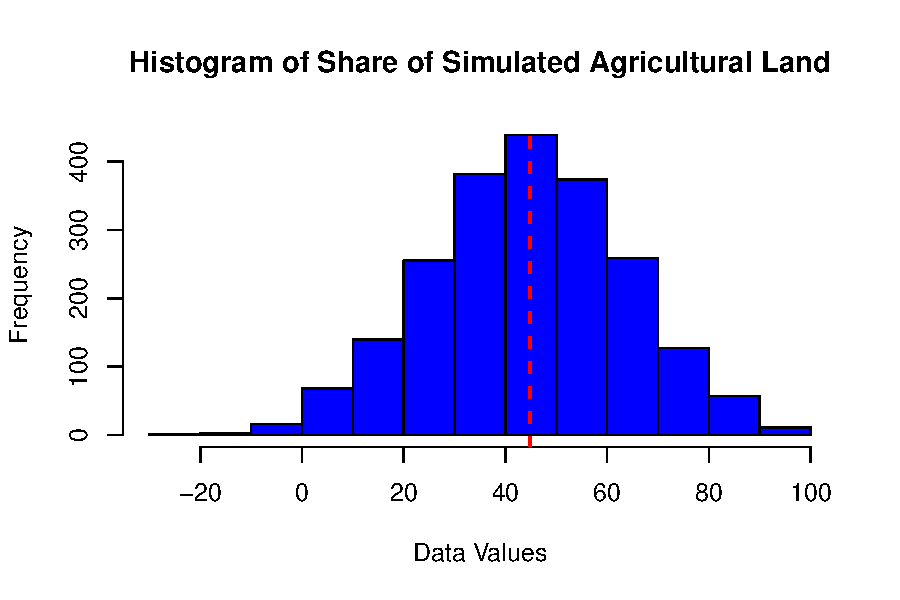
\includegraphics{_main_files/figure-latex/unnamed-chunk-44-1.pdf}

\begin{enumerate}
\def\labelenumi{\roman{enumi}.}
\setcounter{enumi}{8}
\tightlist
\item
  The result from the previous point is consistent with the result of the vote given the urban-rural divide in preferences (i.e., municipalities with more agricultural area had higher participation rates). However, you notice that your comparisons across municipalities are not very rigorous because you are ignoring how important agricultural land is with respect to the whole municipality area. An implication of that is that two municipalities with the same agricultural area could be taken as equally rural while one could have a very big urban area (e.g., Zurich) and the other have a very small one.
\end{enumerate}

Thus to make your analysis across more comparable units, you transform the absolute value of the agricultural area to a relative one: the percentage of the municipal area that is agricultural. Create the variable \texttt{AgricAreaPercent} to represent those transformed values. Regress the turn-out on the newly created variable. Again, do the regression without intercept. Report and interpret the parameter. Also present the corresponding graph.

Write the regression here.

\begin{Shaded}
\begin{Highlighting}[]
\CommentTok{\#Transform the units to make them comparable }
\NormalTok{CO2\_land }\OtherTok{\textless{}{-}}\NormalTok{ CO2\_land }\SpecialCharTok{\%\textgreater{}\%}
  \FunctionTok{mutate}\NormalTok{(}\AttributeTok{AgricAreaPercent=} \DecValTok{100}\SpecialCharTok{*}\NormalTok{AgriculturalAreaHa}\SpecialCharTok{/}\NormalTok{TotalAreaHa)}

\CommentTok{\#regression}
\NormalTok{result0 }\OtherTok{\textless{}{-}} \FunctionTok{lm}\NormalTok{(stimmbeteiligungInProzent }\SpecialCharTok{\textasciitilde{}}\NormalTok{ AgricAreaPercent , }\AttributeTok{data =}\NormalTok{ CO2\_land)}
\FunctionTok{summary}\NormalTok{(result0)}
\end{Highlighting}
\end{Shaded}

\begin{verbatim}
## 
## Call:
## lm(formula = stimmbeteiligungInProzent ~ AgricAreaPercent, data = CO2_land)
## 
## Residuals:
##     Min      1Q  Median      3Q     Max 
## -19.971  -4.760  -0.270   4.314  39.145 
## 
## Coefficients:
##                   Estimate Std. Error t value Pr(>|t|)    
## (Intercept)      55.189867   0.384603   143.5   <2e-16 ***
## AgricAreaPercent  0.219491   0.007894    27.8   <2e-16 ***
## ---
## Signif. codes:  0 '***' 0.001 '**' 0.01 '*' 0.05 '.' 0.1 ' ' 1
## 
## Residual standard error: 6.969 on 2130 degrees of freedom
## Multiple R-squared:  0.2663, Adjusted R-squared:  0.2659 
## F-statistic: 773.1 on 1 and 2130 DF,  p-value: < 2.2e-16
\end{verbatim}

Report and interpret the parameter here.

\begin{Shaded}
\begin{Highlighting}[]
\NormalTok{coeffs}\OtherTok{\textless{}{-}} \FunctionTok{coef}\NormalTok{(result0)}
\NormalTok{coeffs}
\end{Highlighting}
\end{Shaded}

\begin{verbatim}
##      (Intercept) AgricAreaPercent 
##        55.189867         0.219491
\end{verbatim}

The estimated (Intercept) is 55.19, while the estimated slope for AgricAreaPercent is 0.22. It means that, across Swiss municipalities an increase of one percentage point in the share of agricultural land was associated with an average increase in the turn-out of 0.22 percentage points.

Present the graph here.

\begin{Shaded}
\begin{Highlighting}[]
\CommentTok{\# Create a scatter plot}
\FunctionTok{ggplot}\NormalTok{(CO2\_land, }\FunctionTok{aes}\NormalTok{(}\AttributeTok{x =}\NormalTok{ AgricAreaPercent, }\AttributeTok{y =}\NormalTok{ stimmbeteiligungInProzent)) }\SpecialCharTok{+}
  \FunctionTok{geom\_point}\NormalTok{() }\SpecialCharTok{+}
  \FunctionTok{geom\_smooth}\NormalTok{(}\AttributeTok{method =} \StringTok{"lm"}\NormalTok{, }\AttributeTok{formula =}\NormalTok{ y }\SpecialCharTok{\textasciitilde{}}\NormalTok{ x, }\AttributeTok{se =} \ConstantTok{FALSE}\NormalTok{, }\AttributeTok{color =} \StringTok{"purple"}\NormalTok{) }\SpecialCharTok{+}  \CommentTok{\# Adding the regression line}
  \FunctionTok{theme\_minimal}\NormalTok{() }\SpecialCharTok{+}
  \FunctionTok{theme}\NormalTok{(}\AttributeTok{plot.title =} \FunctionTok{element\_text}\NormalTok{(}\AttributeTok{hjust =} \FloatTok{0.5}\NormalTok{)) }\SpecialCharTok{+}
  \FunctionTok{labs}\NormalTok{(}
    \AttributeTok{x =} \StringTok{"Agricultural Area (\%)"}\NormalTok{,}
    \AttributeTok{y =} \StringTok{"Turn{-}out (\%)"}\NormalTok{,}
    \AttributeTok{title =} \StringTok{"Scatter plot with Linear Regression Line"}
\NormalTok{  )}
\end{Highlighting}
\end{Shaded}

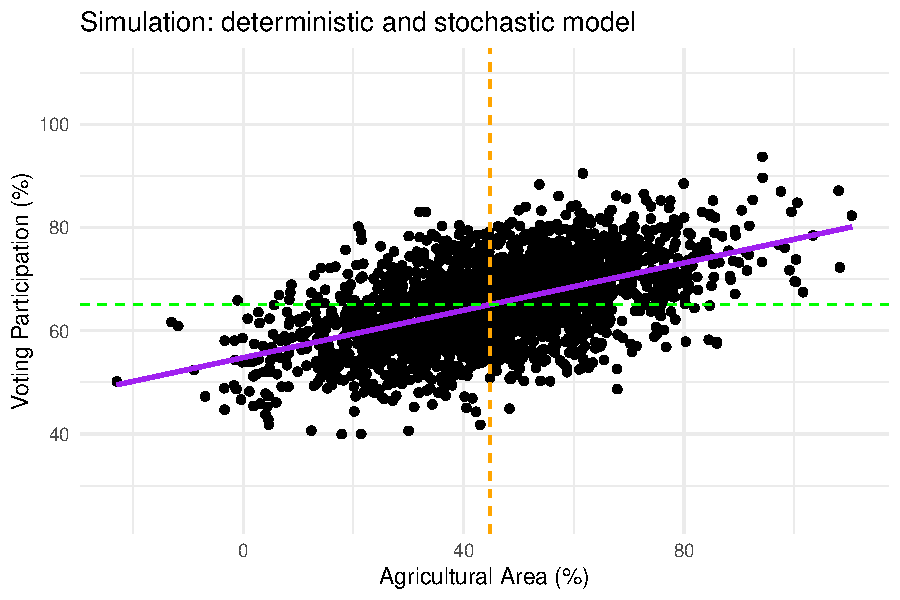
\includegraphics{_main_files/figure-latex/unnamed-chunk-47-1.pdf}

\begin{enumerate}
\def\labelenumi{\alph{enumi}.}
\setcounter{enumi}{23}
\tightlist
\item
  {[}Optional{]} While analyzing your results, you asked yourself: what would have happened with my regression if it is estimated without an intercept? In particular, you asked yourself: does the the distance from each data point to the regression line decrease when an intercept is used? See this \href{https://en.wikipedia.org/wiki/Coefficient_of_determination}{entry}, particularly the graph with the blue and red squares to understand the logic of the R\^{}2 as a measure for goodness of fit. You want to compare both the regression lines with and without the intercept in one same graph. Do it. What lesson can you get from this comparison?
\end{enumerate}

\begin{Shaded}
\begin{Highlighting}[]
\FunctionTok{ggplot}\NormalTok{(CO2\_land, }\FunctionTok{aes}\NormalTok{(}\AttributeTok{x =}\NormalTok{ AgricAreaPercent, }\AttributeTok{y =}\NormalTok{ stimmbeteiligungInProzent)) }\SpecialCharTok{+}
  \FunctionTok{geom\_point}\NormalTok{() }\SpecialCharTok{+}
  \FunctionTok{geom\_smooth}\NormalTok{(}\AttributeTok{method =} \StringTok{"lm"}\NormalTok{, }\AttributeTok{formula =}\NormalTok{ y }\SpecialCharTok{\textasciitilde{}}\NormalTok{ x}\DecValTok{{-}1}\NormalTok{, }\AttributeTok{se =} \ConstantTok{FALSE}\NormalTok{, }\AttributeTok{color =} \StringTok{"red"}\NormalTok{) }\SpecialCharTok{+}  \CommentTok{\# Adding the regression line}
  \FunctionTok{geom\_smooth}\NormalTok{(}\AttributeTok{method =} \StringTok{"lm"}\NormalTok{, }\AttributeTok{formula =}\NormalTok{ y }\SpecialCharTok{\textasciitilde{}}\NormalTok{ x, }\AttributeTok{se =} \ConstantTok{FALSE}\NormalTok{, }\AttributeTok{color =} \StringTok{"purple"}\NormalTok{) }\SpecialCharTok{+}  \CommentTok{\# Adding the regression line}
  \FunctionTok{scale\_y\_continuous}\NormalTok{(}\AttributeTok{limits =} \FunctionTok{c}\NormalTok{(}\DecValTok{25}\NormalTok{, }\FunctionTok{max}\NormalTok{(CO2\_land}\SpecialCharTok{$}\NormalTok{stimmbeteiligungInProzent, }\AttributeTok{na.rm =} \ConstantTok{TRUE}\NormalTok{))) }\SpecialCharTok{+}  \CommentTok{\#}
  \FunctionTok{theme\_minimal}\NormalTok{() }\SpecialCharTok{+}
  \FunctionTok{theme}\NormalTok{(}\AttributeTok{plot.title =} \FunctionTok{element\_text}\NormalTok{(}\AttributeTok{hjust =} \FloatTok{0.5}\NormalTok{)) }\SpecialCharTok{+}
  \FunctionTok{labs}\NormalTok{(}
    \AttributeTok{x =} \StringTok{"Agricultural Area (\%)"}\NormalTok{,}
    \AttributeTok{y =} \StringTok{"Turn{-}out (\%)"}\NormalTok{,}
    \AttributeTok{title =} \StringTok{"Scatter plot with Linear Regression Line"}
\NormalTok{  )}
\end{Highlighting}
\end{Shaded}

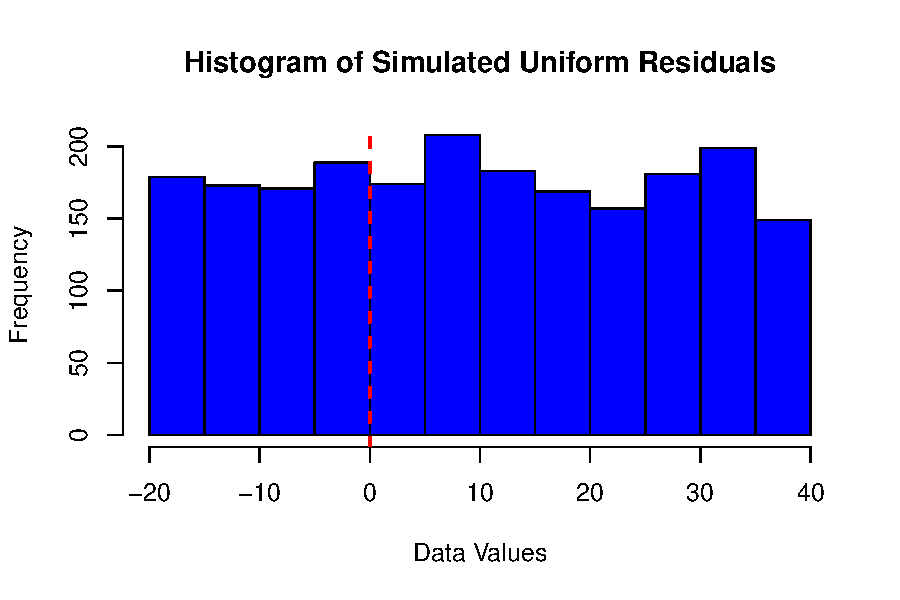
\includegraphics{_main_files/figure-latex/unnamed-chunk-48-1.pdf}

The lesson is that using the intercept is always desirable as it can potentially improve the goodness of fit, while doesn't worsen it (i.e., the optimal intercept could be estimated to be zero). As it is clear from the graph, not using the intercept provides less reliable predictions and general descriptions for the relation between our variables of interest.

\begin{enumerate}
\def\labelenumi{\roman{enumi}.}
\setcounter{enumi}{10}
\tightlist
\item
  {[}Optional{]} Now add a vertical line with the average for the agricultural area, and a horizontal one with the average turn-out. What does this new graph tell you about the descriptive performance of a regression with and without intercepts?
\end{enumerate}

\begin{Shaded}
\begin{Highlighting}[]
\CommentTok{\#Means for Y and X}
\NormalTok{mean\_AgricAreaPercent }\OtherTok{\textless{}{-}} \FunctionTok{mean}\NormalTok{(CO2\_land}\SpecialCharTok{$}\NormalTok{AgricAreaPercent, }\AttributeTok{na.rm =} \ConstantTok{TRUE}\NormalTok{)}
\NormalTok{mean\_stimmbeteiligungInProzent }\OtherTok{\textless{}{-}} \FunctionTok{mean}\NormalTok{(CO2\_land}\SpecialCharTok{$}\NormalTok{stimmbeteiligungInProzent, }\AttributeTok{na.rm =} \ConstantTok{TRUE}\NormalTok{)}

\CommentTok{\# Create a scatter plot}
\FunctionTok{ggplot}\NormalTok{(CO2\_land, }\FunctionTok{aes}\NormalTok{(}\AttributeTok{x =}\NormalTok{ AgricAreaPercent, }\AttributeTok{y =}\NormalTok{ stimmbeteiligungInProzent)) }\SpecialCharTok{+}
  \FunctionTok{geom\_point}\NormalTok{() }\SpecialCharTok{+}
  \FunctionTok{geom\_smooth}\NormalTok{(}\AttributeTok{method =} \StringTok{"lm"}\NormalTok{, }\AttributeTok{formula =}\NormalTok{ y }\SpecialCharTok{\textasciitilde{}}\NormalTok{ x }\SpecialCharTok{{-}} \DecValTok{1}\NormalTok{, }\AttributeTok{se =} \ConstantTok{FALSE}\NormalTok{, }\AttributeTok{color =} \StringTok{"red"}\NormalTok{) }\SpecialCharTok{+}  \CommentTok{\# Adding the regression line}
  \FunctionTok{geom\_smooth}\NormalTok{(}\AttributeTok{method =} \StringTok{"lm"}\NormalTok{, }\AttributeTok{formula =}\NormalTok{ y }\SpecialCharTok{\textasciitilde{}}\NormalTok{ x, }\AttributeTok{se =} \ConstantTok{FALSE}\NormalTok{, }\AttributeTok{color =} \StringTok{"purple"}\NormalTok{) }\SpecialCharTok{+}  \CommentTok{\# Adding the regression line}
  \FunctionTok{geom\_hline}\NormalTok{(}\AttributeTok{yintercept =}\NormalTok{ mean\_stimmbeteiligungInProzent, }\AttributeTok{linetype =} \StringTok{"dashed"}\NormalTok{, }\AttributeTok{color =} \StringTok{"green"}\NormalTok{) }\SpecialCharTok{+}  \CommentTok{\# Horizontal line at the mean of y}
  \FunctionTok{geom\_vline}\NormalTok{(}\AttributeTok{xintercept =}\NormalTok{ mean\_AgricAreaPercent, }\AttributeTok{linetype =} \StringTok{"dashed"}\NormalTok{, }\AttributeTok{color =} \StringTok{"orange"}\NormalTok{) }\SpecialCharTok{+}  \CommentTok{\# Vertical line at the mean of x}
  \FunctionTok{scale\_y\_continuous}\NormalTok{(}\AttributeTok{limits =} \FunctionTok{c}\NormalTok{(}\DecValTok{25}\NormalTok{, }\FunctionTok{max}\NormalTok{(CO2\_land}\SpecialCharTok{$}\NormalTok{stimmbeteiligungInProzent, }\AttributeTok{na.rm =} \ConstantTok{TRUE}\NormalTok{))) }\SpecialCharTok{+}  \CommentTok{\#}
  \FunctionTok{theme\_minimal}\NormalTok{() }\SpecialCharTok{+}
  \FunctionTok{theme}\NormalTok{(}\AttributeTok{plot.title =} \FunctionTok{element\_text}\NormalTok{(}\AttributeTok{hjust =} \FloatTok{0.5}\NormalTok{)) }\SpecialCharTok{+}
  \FunctionTok{labs}\NormalTok{(}
    \AttributeTok{x =} \StringTok{"Agricultural Area (\%)"}\NormalTok{,}
    \AttributeTok{y =} \StringTok{"Turn{-}out (\%)"}\NormalTok{,}
    \AttributeTok{title =} \StringTok{"Scatter plot with Linear Regression Line"}
\NormalTok{  )}
\end{Highlighting}
\end{Shaded}

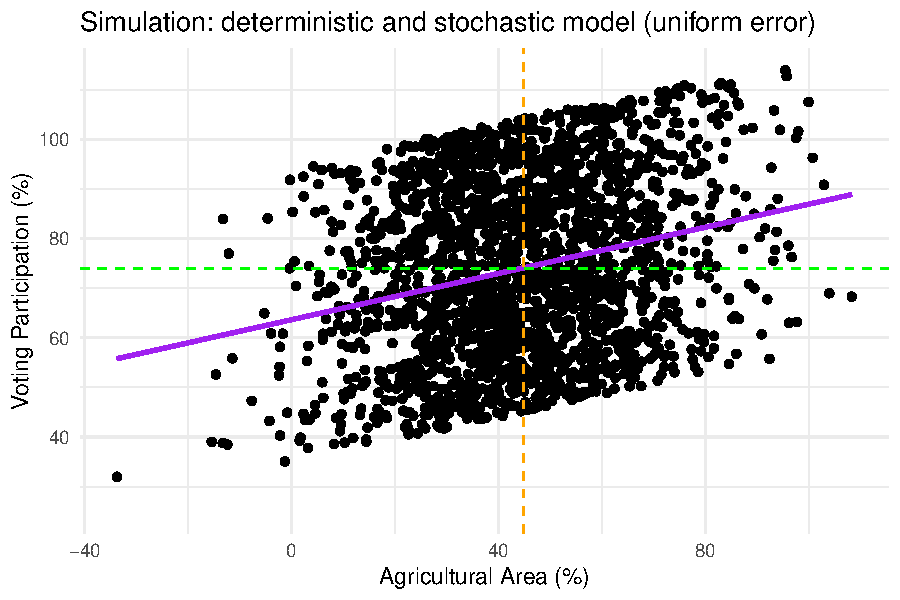
\includegraphics{_main_files/figure-latex/unnamed-chunk-49-1.pdf}
The descriptive performance of a regression with an intercept is better than without it. As the graph shows, the vertical and horizontal lines for the averages of the dependent and independent variables overlap with each other in exactly the same place where the regression line with intercept goes through. This shows the capability of single linear regression to capture central tendency of the fitted data. On the contrary, the regression without intercept does not do that. Once again, this shows how the descriptive performance of a regression with intercept captures more intuitively the general relation between one variable and another.

\begin{enumerate}
\def\labelenumi{\roman{enumi}.}
\setcounter{enumi}{11}
\tightlist
\item
  Store the residuals as \texttt{residuals}. Plot the share of agricultural area against the residuals. What does it tell you regarding the ability of the model to describe the central tendency of the relationship across all values of the agricultural land share?
\end{enumerate}

\begin{Shaded}
\begin{Highlighting}[]
\NormalTok{residuals0 }\OtherTok{\textless{}{-}} \FunctionTok{residuals}\NormalTok{(result0)}

\FunctionTok{ggplot}\NormalTok{(CO2\_land, }\FunctionTok{aes}\NormalTok{(}\AttributeTok{x =}\NormalTok{ AgricAreaPercent, }\AttributeTok{y =}\NormalTok{ residuals0)) }\SpecialCharTok{+}
  \FunctionTok{geom\_point}\NormalTok{() }\SpecialCharTok{+}
  \FunctionTok{geom\_smooth}\NormalTok{(}\AttributeTok{method =} \StringTok{"lm"}\NormalTok{, }\AttributeTok{formula =}\NormalTok{ y }\SpecialCharTok{\textasciitilde{}}\NormalTok{ x , }\AttributeTok{se =} \ConstantTok{TRUE}\NormalTok{, }\AttributeTok{color =} \StringTok{"green"}\NormalTok{)}\SpecialCharTok{+}  \CommentTok{\# Adding the}
  \FunctionTok{theme\_minimal}\NormalTok{() }\SpecialCharTok{+}
  \FunctionTok{theme}\NormalTok{(}\AttributeTok{plot.title =} \FunctionTok{element\_text}\NormalTok{(}\AttributeTok{hjust =} \FloatTok{0.5}\NormalTok{)) }\SpecialCharTok{+}
  \FunctionTok{labs}\NormalTok{(}
    \AttributeTok{x =} \StringTok{"Agricultural Area (\%)"}\NormalTok{,}
    \AttributeTok{y =} \StringTok{"Residuals (turn{-}out p.p.)"}\NormalTok{,}
    \AttributeTok{title =} \StringTok{"Scatter plot with Linear Regression Line"}
\NormalTok{  )}
\end{Highlighting}
\end{Shaded}

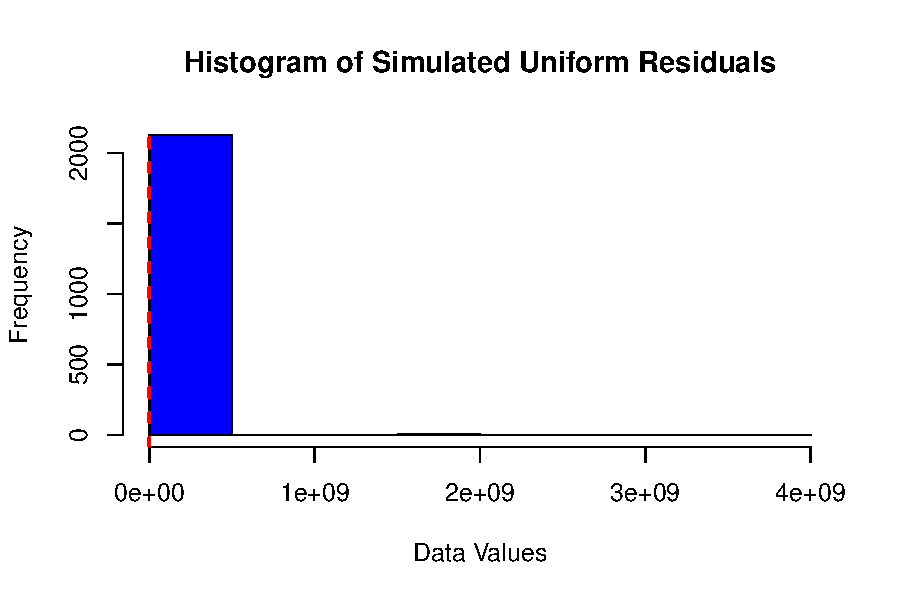
\includegraphics{_main_files/figure-latex/unnamed-chunk-50-1.pdf}
The existence of a horizontal slope between the residuals (i.e., the distance between the prediction and the real value) and the agricultural share suggests that our model has systematically captured the relation between our variables: the average error does not not change systematically across the values of the agricultural share.

\begin{enumerate}
\def\labelenumi{\roman{enumi}.}
\setcounter{enumi}{12}
\tightlist
\item
  {[}Optional{]} Repeat the previous point without the intercept. Does the linear regression remains a good tool for describing the central tendency of the relationship across all values of the agricultural land share?
\end{enumerate}

\begin{Shaded}
\begin{Highlighting}[]
\CommentTok{\#regression}
\NormalTok{result1 }\OtherTok{\textless{}{-}} \FunctionTok{lm}\NormalTok{(stimmbeteiligungInProzent }\SpecialCharTok{\textasciitilde{}}\NormalTok{ AgricAreaPercent }\SpecialCharTok{{-}}\DecValTok{1}\NormalTok{ , }\AttributeTok{data =}\NormalTok{ CO2\_land)}
\FunctionTok{summary}\NormalTok{(result1)}
\end{Highlighting}
\end{Shaded}

\begin{verbatim}
## 
## Call:
## lm(formula = stimmbeteiligungInProzent ~ AgricAreaPercent - 1, 
##     data = CO2_land)
## 
## Residuals:
##     Min      1Q  Median      3Q     Max 
## -42.102  -7.509   6.449  23.631  83.331 
## 
## Coefficients:
##                  Estimate Std. Error t value Pr(>|t|)    
## AgricAreaPercent  1.26144    0.01012   124.7   <2e-16 ***
## ---
## Signif. codes:  0 '***' 0.001 '**' 0.01 '*' 0.05 '.' 0.1 ' ' 1
## 
## Residual standard error: 22.75 on 2131 degrees of freedom
## Multiple R-squared:  0.8795, Adjusted R-squared:  0.8794 
## F-statistic: 1.555e+04 on 1 and 2131 DF,  p-value: < 2.2e-16
\end{verbatim}

\begin{Shaded}
\begin{Highlighting}[]
\NormalTok{residuals1 }\OtherTok{\textless{}{-}} \FunctionTok{residuals}\NormalTok{(result1)}

\FunctionTok{ggplot}\NormalTok{(CO2\_land, }\FunctionTok{aes}\NormalTok{(}\AttributeTok{x =}\NormalTok{ AgricAreaPercent, }\AttributeTok{y =}\NormalTok{ residuals1)) }\SpecialCharTok{+}
  \FunctionTok{geom\_point}\NormalTok{() }\SpecialCharTok{+}
  \FunctionTok{geom\_smooth}\NormalTok{(}\AttributeTok{method =} \StringTok{"lm"}\NormalTok{, }\AttributeTok{formula =}\NormalTok{ y }\SpecialCharTok{\textasciitilde{}}\NormalTok{ x , }\AttributeTok{se =} \ConstantTok{TRUE}\NormalTok{, }\AttributeTok{color =} \StringTok{"red"}\NormalTok{)}\SpecialCharTok{+}  \CommentTok{\# Adding the}
  \FunctionTok{theme\_minimal}\NormalTok{() }\SpecialCharTok{+}
  \FunctionTok{theme}\NormalTok{(}\AttributeTok{plot.title =} \FunctionTok{element\_text}\NormalTok{(}\AttributeTok{hjust =} \FloatTok{0.5}\NormalTok{)) }\SpecialCharTok{+}
  \FunctionTok{labs}\NormalTok{(}
    \AttributeTok{x =} \StringTok{"Agricultural Area (\%)"}\NormalTok{,}
    \AttributeTok{y =} \StringTok{"Residuals (turn{-}out p.p.)"}\NormalTok{,}
    \AttributeTok{title =} \StringTok{"Scatter plot with Linear Regression Line"}
\NormalTok{  )}
\end{Highlighting}
\end{Shaded}

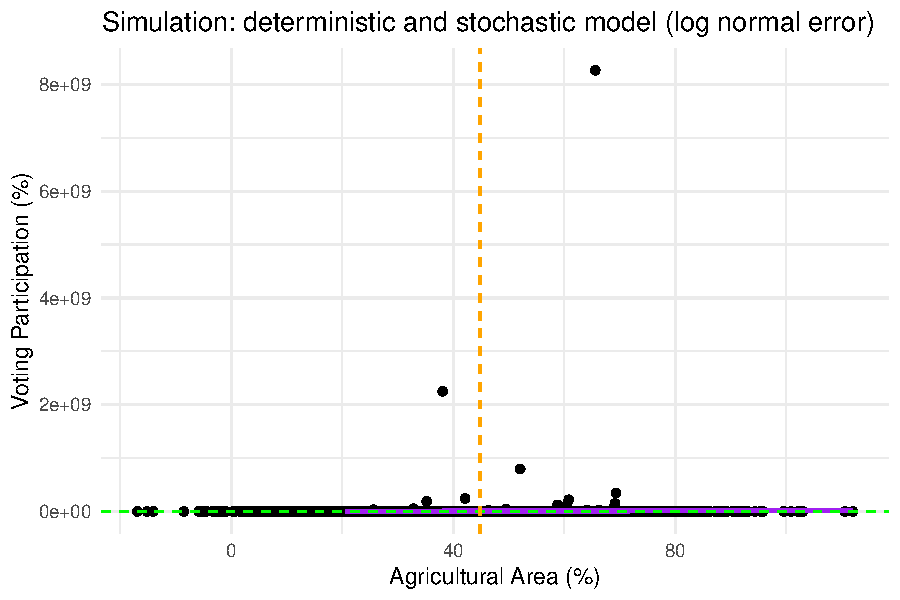
\includegraphics{_main_files/figure-latex/unnamed-chunk-51-1.pdf}

Unlike the graph of the previous point showed that no systematic relation between the residual and our regressor was not captured by our model, the graph of this point shows a systematic behavior of the residuals. In this case, it is the fact that the model is too inflexible (i.e., the line must always go through the origin) which leads the model to predict the values of our regressand in a systematically mistaken way: the average error does change systematically across the values of the agricultural share, being systematically positive for lower age values, while systematically negative for high age values.

\hypertarget{simulated-data}{%
\subsection{Simulated data}\label{simulated-data}}

\begin{enumerate}
\def\labelenumi{\roman{enumi}.}
\tightlist
\item
  You will now simulate the relationship between turn-out and share of agricultural land. Assume the parameters estimated in the last regression (i.e., the \(\beta_0\) and \(\beta_1\)). Retrieve both parameters.
\end{enumerate}

\begin{Shaded}
\begin{Highlighting}[]
\NormalTok{coeffs}\OtherTok{\textless{}{-}} \FunctionTok{coef}\NormalTok{(result0)}
\FunctionTok{print}\NormalTok{(coeffs)}
\end{Highlighting}
\end{Shaded}

\begin{verbatim}
##      (Intercept) AgricAreaPercent 
##        55.189867         0.219491
\end{verbatim}

\begin{Shaded}
\begin{Highlighting}[]
\FunctionTok{print}\NormalTok{(}\FunctionTok{unname}\NormalTok{(coeffs[}\DecValTok{1}\NormalTok{]), }\AttributeTok{digits =} \DecValTok{2}\NormalTok{)}
\end{Highlighting}
\end{Shaded}

\begin{verbatim}
## [1] 55
\end{verbatim}

\begin{Shaded}
\begin{Highlighting}[]
\FunctionTok{print}\NormalTok{(}\FunctionTok{unname}\NormalTok{(coeffs[}\DecValTok{2}\NormalTok{]), }\AttributeTok{digits =} \DecValTok{2}\NormalTok{)}
\end{Highlighting}
\end{Shaded}

\begin{verbatim}
## [1] 0.22
\end{verbatim}

\begin{enumerate}
\def\labelenumi{\roman{enumi}.}
\setcounter{enumi}{1}
\tightlist
\item
  Use the parameters to define the assumed data generating process. Assume that the process is deterministic (i.e., it has no stochastic component). Express the equation using mathematical notation.
\end{enumerate}

\[TurnOut_i = \beta_0 + \beta_1 * ShareAgriculturalLand\]

\begin{enumerate}
\def\labelenumi{\roman{enumi}.}
\setcounter{enumi}{2}
\tightlist
\item
  Generate a normal distribution that preserves the mean and standard deviation of the original data on share of agricultural land.
\end{enumerate}

\begin{Shaded}
\begin{Highlighting}[]
\FunctionTok{set.seed}\NormalTok{(}\DecValTok{123}\NormalTok{) }\CommentTok{\# to ensure reproducibility: should different people use different random draws, the results won\textquotesingle{}t be consistent. Thus, should all use the same random draw, all should have the same results.}
\NormalTok{CO2\_land}\SpecialCharTok{$}\NormalTok{Sim\_ShareAgric\_norm }\OtherTok{\textless{}{-}} \FunctionTok{rnorm}\NormalTok{(}\FunctionTok{nrow}\NormalTok{(CO2\_land), }\AttributeTok{mean =}\NormalTok{ mean\_AgricAreaPercent, }\AttributeTok{sd =} \FunctionTok{sd}\NormalTok{(CO2\_land}\SpecialCharTok{$}\NormalTok{AgricAreaPercent))}

\FunctionTok{hist}\NormalTok{(CO2\_land}\SpecialCharTok{$}\NormalTok{Sim\_ShareAgric\_norm, }
     \AttributeTok{main=}\StringTok{"Histogram of Share of Simulated Agricultural Land"}\NormalTok{, }
     \AttributeTok{xlab=}\StringTok{"Data Values"}\NormalTok{, }
     \AttributeTok{ylab=}\StringTok{"Frequency"}\NormalTok{, }
     \AttributeTok{col=}\StringTok{"blue"}\NormalTok{, }
     \AttributeTok{border=}\StringTok{"black"}\NormalTok{)}

\FunctionTok{abline}\NormalTok{(}\AttributeTok{v=}\NormalTok{mean\_AgricAreaPercent, }\AttributeTok{col=}\StringTok{"red"}\NormalTok{, }\AttributeTok{lwd=}\DecValTok{2}\NormalTok{, }\AttributeTok{lty=}\DecValTok{2}\NormalTok{)}
\end{Highlighting}
\end{Shaded}

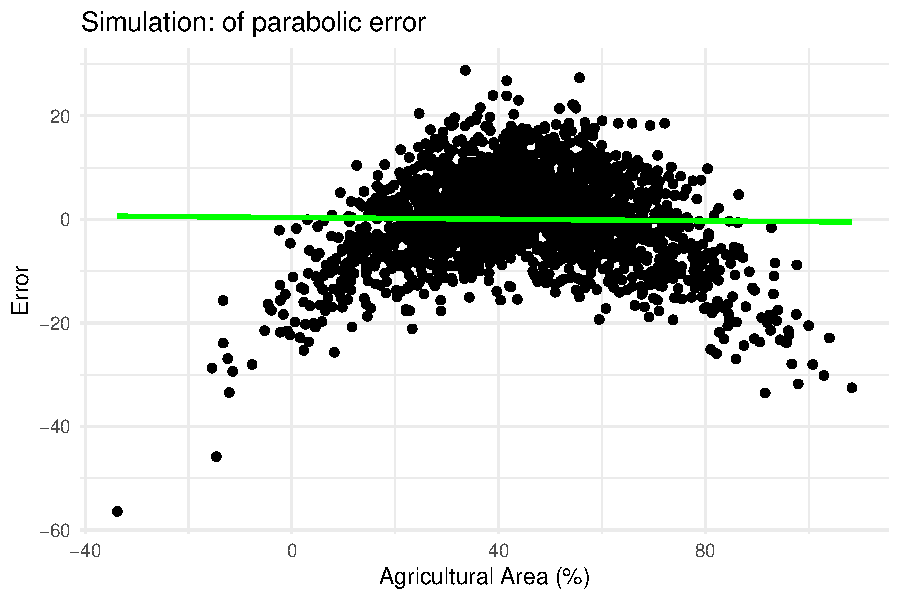
\includegraphics{_main_files/figure-latex/unnamed-chunk-53-1.pdf}

\begin{enumerate}
\def\labelenumi{\roman{enumi}.}
\setcounter{enumi}{3}
\tightlist
\item
  Predict the turn-out values given the simulated inputs on the share of agricultural land using the data generating process defined in point i). Graph relation between both variables using a liner regression line.
\end{enumerate}

\begin{Shaded}
\begin{Highlighting}[]
\NormalTok{CO2\_land}\SpecialCharTok{$}\NormalTok{Pred\_TurnOut\_Determ }\OtherTok{\textless{}{-}} \FunctionTok{unname}\NormalTok{(coeffs[}\DecValTok{1}\NormalTok{]) }\SpecialCharTok{+} \FunctionTok{unname}\NormalTok{(coeffs[}\DecValTok{2}\NormalTok{])}\SpecialCharTok{*}\NormalTok{CO2\_land}\SpecialCharTok{$}\NormalTok{Sim\_ShareAgric\_norm}


\FunctionTok{ggplot}\NormalTok{(CO2\_land, }\FunctionTok{aes}\NormalTok{(}\AttributeTok{x =}\NormalTok{ Sim\_ShareAgric\_norm, }\AttributeTok{y =}\NormalTok{ Pred\_TurnOut\_Determ)) }\SpecialCharTok{+}
  \FunctionTok{geom\_point}\NormalTok{() }\SpecialCharTok{+}
  \FunctionTok{geom\_smooth}\NormalTok{(}\AttributeTok{method =} \StringTok{"lm"}\NormalTok{, }\AttributeTok{formula =}\NormalTok{ y }\SpecialCharTok{\textasciitilde{}}\NormalTok{ x, }\AttributeTok{se =} \ConstantTok{FALSE}\NormalTok{, }\AttributeTok{color =} \StringTok{"purple"}\NormalTok{) }\SpecialCharTok{+}  \CommentTok{\# Adding the regression line}
  \FunctionTok{geom\_hline}\NormalTok{(}\AttributeTok{yintercept =}\NormalTok{ mean\_stimmbeteiligungInProzent, }\AttributeTok{linetype =} \StringTok{"dashed"}\NormalTok{, }\AttributeTok{color =} \StringTok{"green"}\NormalTok{) }\SpecialCharTok{+}  \CommentTok{\# Horizontal line at the mean of y}
  \FunctionTok{geom\_vline}\NormalTok{(}\AttributeTok{xintercept =}\NormalTok{ mean\_AgricAreaPercent, }\AttributeTok{linetype =} \StringTok{"dashed"}\NormalTok{, }\AttributeTok{color =} \StringTok{"orange"}\NormalTok{) }\SpecialCharTok{+}  \CommentTok{\# Vertical line at the mean of x}
  \FunctionTok{scale\_y\_continuous}\NormalTok{(}\AttributeTok{limits =} \FunctionTok{c}\NormalTok{(}\DecValTok{25}\NormalTok{, }\FunctionTok{max}\NormalTok{(CO2\_land}\SpecialCharTok{$}\NormalTok{stimmbeteiligungInProzent, }\AttributeTok{na.rm =} \ConstantTok{TRUE}\NormalTok{))) }\SpecialCharTok{+}  \CommentTok{\#}
  \FunctionTok{theme\_minimal}\NormalTok{() }\SpecialCharTok{+}
  \FunctionTok{theme}\NormalTok{(}\AttributeTok{plot.title =} \FunctionTok{element\_text}\NormalTok{(}\AttributeTok{hjust =} \FloatTok{0.5}\NormalTok{)) }\SpecialCharTok{+}
  \FunctionTok{labs}\NormalTok{(}
    \AttributeTok{x =} \StringTok{"Agricultural Area (\%)"}\NormalTok{,}
    \AttributeTok{y =} \StringTok{"Turn{-}out (\%)"}\NormalTok{,}
    \AttributeTok{title =} \StringTok{"Simulation: deterministic model"}
\NormalTok{  )}
\end{Highlighting}
\end{Shaded}

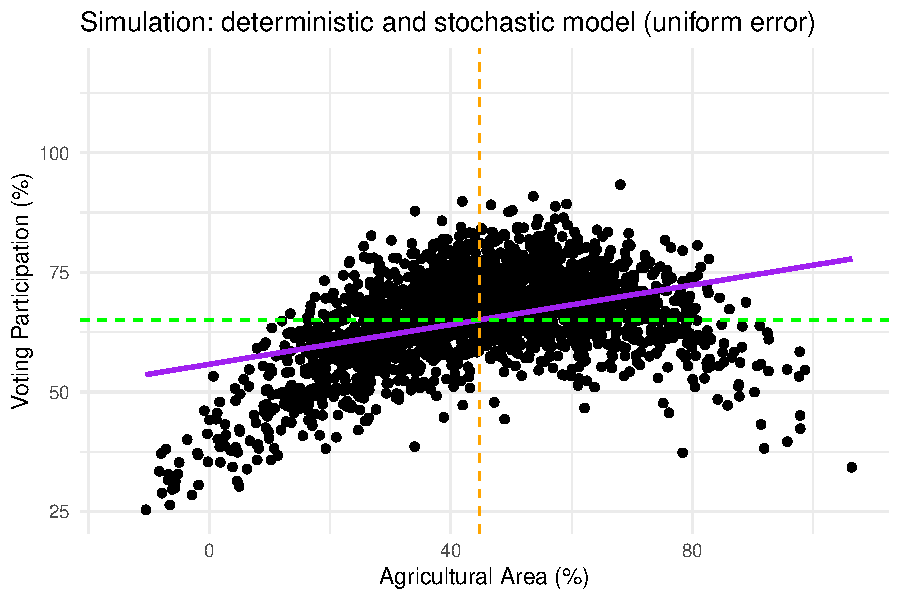
\includegraphics{_main_files/figure-latex/unnamed-chunk-54-1.pdf}
As expected, this deterministic model generates points on top of the regression line defined by the intercept and slope of the data generating process. Unlike in reality, we have no random errors generating random deviations from the regression line (i.e., we have no cloud of points, but they are all on top of the line).

\begin{enumerate}
\def\labelenumi{\alph{enumi}.}
\setcounter{enumi}{21}
\tightlist
\item
  Generate a normal distribution with error distribution with mean zero and standard deviation equal to the standard deviation of the residual of the model with intercept.
\end{enumerate}

\begin{Shaded}
\begin{Highlighting}[]
\FunctionTok{set.seed}\NormalTok{(}\DecValTok{123}\NormalTok{)}
\NormalTok{CO2\_land}\SpecialCharTok{$}\NormalTok{Sim\_resid\_norm }\OtherTok{\textless{}{-}} \FunctionTok{rnorm}\NormalTok{(}\FunctionTok{nrow}\NormalTok{(CO2\_land), }\AttributeTok{mean =} \DecValTok{0}\NormalTok{, }\AttributeTok{sd =} \FunctionTok{sd}\NormalTok{(residuals0))}

\FunctionTok{hist}\NormalTok{(CO2\_land}\SpecialCharTok{$}\NormalTok{Sim\_resid\_norm, }
     \AttributeTok{main=}\StringTok{"Histogram of Simulated Normal Residuals"}\NormalTok{, }
     \AttributeTok{xlab=}\StringTok{"Data Values"}\NormalTok{, }
     \AttributeTok{ylab=}\StringTok{"Frequency"}\NormalTok{, }
     \AttributeTok{col=}\StringTok{"blue"}\NormalTok{, }
     \AttributeTok{border=}\StringTok{"black"}\NormalTok{)}

\FunctionTok{abline}\NormalTok{(}\AttributeTok{v=}\DecValTok{0}\NormalTok{, }\AttributeTok{col=}\StringTok{"red"}\NormalTok{, }\AttributeTok{lwd=}\DecValTok{2}\NormalTok{, }\AttributeTok{lty=}\DecValTok{2}\NormalTok{)}
\end{Highlighting}
\end{Shaded}

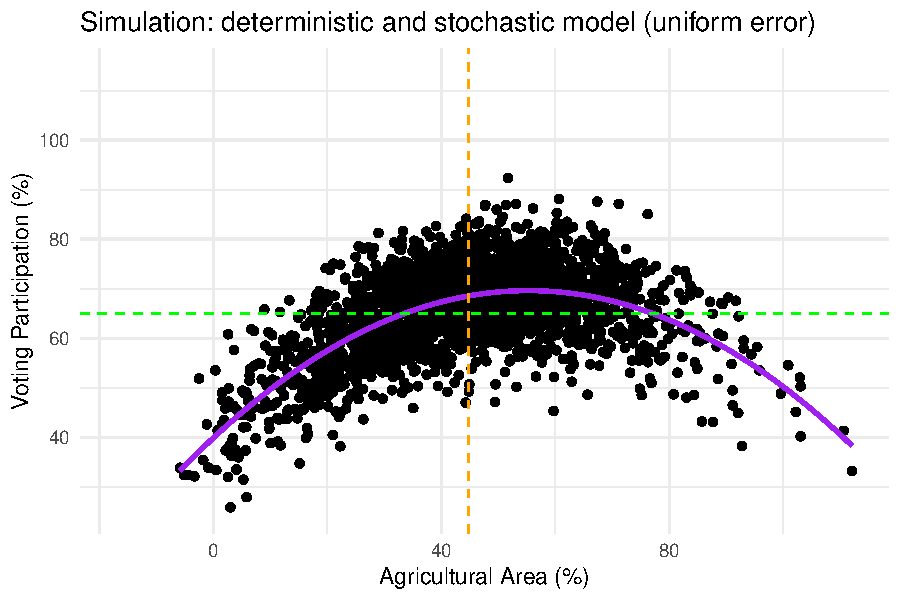
\includegraphics{_main_files/figure-latex/unnamed-chunk-55-1.pdf}

\begin{enumerate}
\def\labelenumi{\roman{enumi}.}
\setcounter{enumi}{5}
\tightlist
\item
  Now add the stochastic element to the fully deterministic model of point iv). Graph the relation between both variables using a liner regression line.
\end{enumerate}

\begin{Shaded}
\begin{Highlighting}[]
\NormalTok{CO2\_land}\SpecialCharTok{$}\NormalTok{Pred\_TurnOut\_Stoch }\OtherTok{\textless{}{-}}\NormalTok{ CO2\_land}\SpecialCharTok{$}\NormalTok{Pred\_TurnOut\_Determ }\SpecialCharTok{+}\NormalTok{ CO2\_land}\SpecialCharTok{$}\NormalTok{Sim\_resid\_norm}

\FunctionTok{ggplot}\NormalTok{(CO2\_land, }\FunctionTok{aes}\NormalTok{(}\AttributeTok{x =}\NormalTok{ Sim\_ShareAgric\_norm, }\AttributeTok{y =}\NormalTok{ Pred\_TurnOut\_Stoch)) }\SpecialCharTok{+}
  \FunctionTok{geom\_point}\NormalTok{() }\SpecialCharTok{+}
  \FunctionTok{geom\_smooth}\NormalTok{(}\AttributeTok{method =} \StringTok{"lm"}\NormalTok{, }\AttributeTok{formula =}\NormalTok{ y }\SpecialCharTok{\textasciitilde{}}\NormalTok{ x, }\AttributeTok{se =} \ConstantTok{FALSE}\NormalTok{, }\AttributeTok{color =} \StringTok{"purple"}\NormalTok{) }\SpecialCharTok{+}  \CommentTok{\# Adding the regression line}
  \FunctionTok{geom\_hline}\NormalTok{(}\AttributeTok{yintercept =}\NormalTok{ mean\_stimmbeteiligungInProzent, }\AttributeTok{linetype =} \StringTok{"dashed"}\NormalTok{, }\AttributeTok{color =} \StringTok{"green"}\NormalTok{) }\SpecialCharTok{+}  \CommentTok{\# Horizontal line at the mean of y}
  \FunctionTok{geom\_vline}\NormalTok{(}\AttributeTok{xintercept =}\NormalTok{ mean\_AgricAreaPercent, }\AttributeTok{linetype =} \StringTok{"dashed"}\NormalTok{, }\AttributeTok{color =} \StringTok{"orange"}\NormalTok{) }\SpecialCharTok{+}  \CommentTok{\# Vertical line at the mean of x}
  \FunctionTok{scale\_y\_continuous}\NormalTok{(}\AttributeTok{limits =} \FunctionTok{c}\NormalTok{(}\DecValTok{25}\NormalTok{, }\FunctionTok{max}\NormalTok{(CO2\_land}\SpecialCharTok{$}\NormalTok{Sim\_ShareAgric\_norm, }\AttributeTok{na.rm =} \ConstantTok{TRUE}\NormalTok{))) }\SpecialCharTok{+}  \CommentTok{\#}
  \FunctionTok{theme\_minimal}\NormalTok{() }\SpecialCharTok{+}
  \FunctionTok{theme}\NormalTok{(}\AttributeTok{plot.title =} \FunctionTok{element\_text}\NormalTok{(}\AttributeTok{hjust =} \FloatTok{0.5}\NormalTok{)) }\SpecialCharTok{+}
  \FunctionTok{labs}\NormalTok{(}
    \AttributeTok{x =} \StringTok{"Agricultural Area (\%)"}\NormalTok{,}
    \AttributeTok{y =} \StringTok{"Turn{-}out (\%)"}\NormalTok{,}
    \AttributeTok{title =} \StringTok{"Simulation: deterministic and stochastic model"}
\NormalTok{  )}
\end{Highlighting}
\end{Shaded}

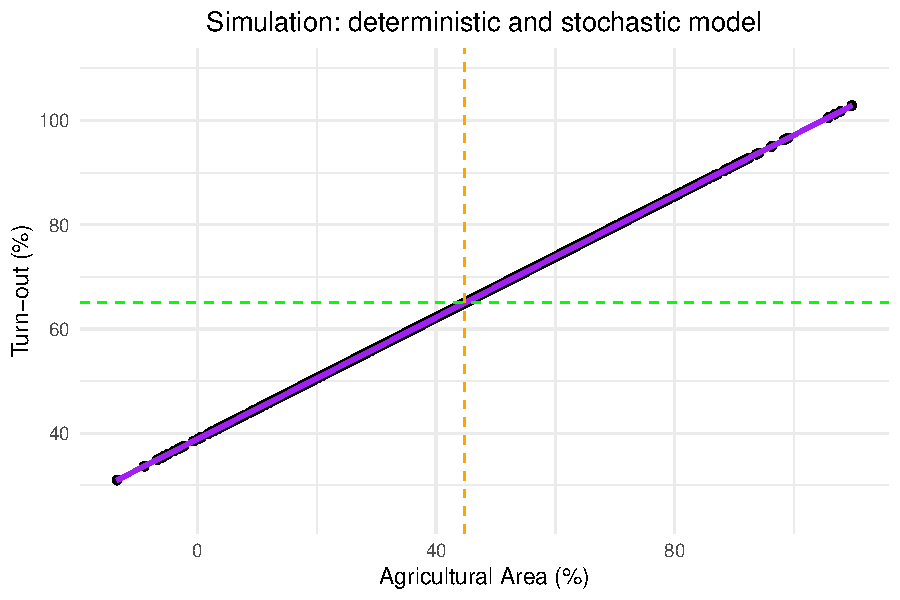
\includegraphics{_main_files/figure-latex/unnamed-chunk-56-1.pdf}
The previous graph presents the relation between our simulated independent variable and residual, both of which fully generate our dependent variable (i.e., only using the regression parameters to predict the observations over the line and then adding the residuals we can generate all the values for our dependent variable).

\begin{enumerate}
\def\labelenumi{\roman{enumi}.}
\setcounter{enumi}{6}
\tightlist
\item
  {[}Optional{]} Now repeat the same simulation but generating errors that distribute uniformly. Use the maximum, and minimum values of the residuals for the model with intercept to define the distribution of residuals.
\end{enumerate}

Uniform simulated residuals:

\begin{Shaded}
\begin{Highlighting}[]
\FunctionTok{set.seed}\NormalTok{(}\DecValTok{123}\NormalTok{)}
\NormalTok{CO2\_land}\SpecialCharTok{$}\NormalTok{Sim\_resid\_unif }\OtherTok{\textless{}{-}} \FunctionTok{runif}\NormalTok{(}\FunctionTok{nrow}\NormalTok{(CO2\_land), }\AttributeTok{min =} \FunctionTok{min}\NormalTok{(residuals0), }\AttributeTok{max =} \FunctionTok{max}\NormalTok{(residuals0))}

\FunctionTok{hist}\NormalTok{(CO2\_land}\SpecialCharTok{$}\NormalTok{Sim\_resid\_unif, }
     \AttributeTok{main=}\StringTok{"Histogram of Simulated Uniform Residuals"}\NormalTok{, }
     \AttributeTok{xlab=}\StringTok{"Data Values"}\NormalTok{, }
     \AttributeTok{ylab=}\StringTok{"Frequency"}\NormalTok{, }
     \AttributeTok{col=}\StringTok{"blue"}\NormalTok{, }
     \AttributeTok{border=}\StringTok{"black"}\NormalTok{)}

\FunctionTok{abline}\NormalTok{(}\AttributeTok{v=}\DecValTok{0}\NormalTok{, }\AttributeTok{col=}\StringTok{"red"}\NormalTok{, }\AttributeTok{lwd=}\DecValTok{2}\NormalTok{, }\AttributeTok{lty=}\DecValTok{2}\NormalTok{)}
\end{Highlighting}
\end{Shaded}

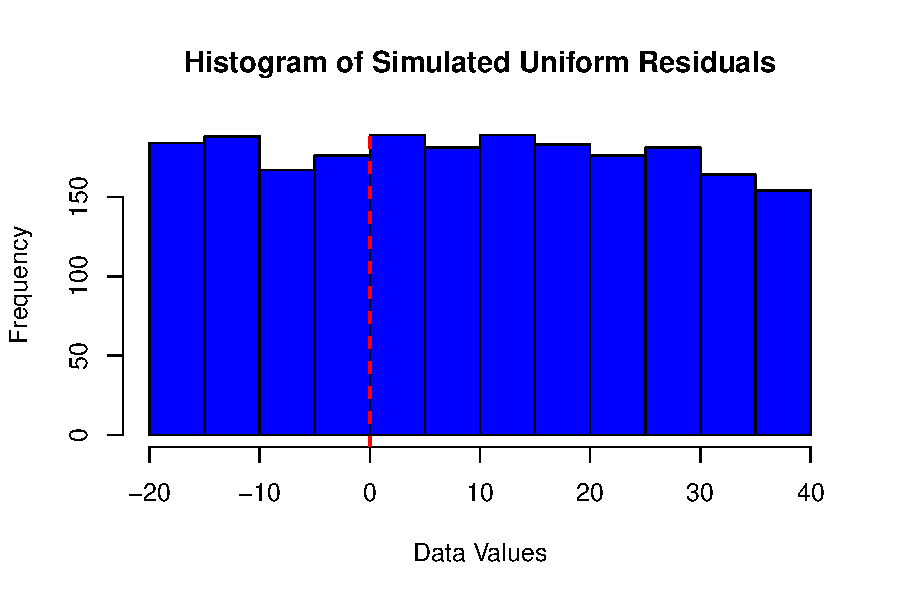
\includegraphics{_main_files/figure-latex/unnamed-chunk-57-1.pdf}

Data generating process with uniform residuals:

\begin{Shaded}
\begin{Highlighting}[]
\NormalTok{CO2\_land}\SpecialCharTok{$}\NormalTok{Pred\_TurnOut\_Unif }\OtherTok{\textless{}{-}}\NormalTok{ CO2\_land}\SpecialCharTok{$}\NormalTok{Pred\_TurnOut\_Determ }\SpecialCharTok{+}\NormalTok{ CO2\_land}\SpecialCharTok{$}\NormalTok{Sim\_resid\_unif}



\FunctionTok{ggplot}\NormalTok{(CO2\_land, }\FunctionTok{aes}\NormalTok{(}\AttributeTok{x =}\NormalTok{ Sim\_ShareAgric\_norm, }\AttributeTok{y =}\NormalTok{ Pred\_TurnOut\_Unif)) }\SpecialCharTok{+}
  \FunctionTok{geom\_point}\NormalTok{() }\SpecialCharTok{+}
  \FunctionTok{geom\_smooth}\NormalTok{(}\AttributeTok{method =} \StringTok{"lm"}\NormalTok{, }\AttributeTok{formula =}\NormalTok{ y }\SpecialCharTok{\textasciitilde{}}\NormalTok{ x, }\AttributeTok{se =} \ConstantTok{FALSE}\NormalTok{, }\AttributeTok{color =} \StringTok{"purple"}\NormalTok{) }\SpecialCharTok{+} 
  \FunctionTok{geom\_hline}\NormalTok{(}\AttributeTok{yintercept =} \FunctionTok{mean}\NormalTok{(CO2\_land}\SpecialCharTok{$}\NormalTok{Pred\_TurnOut\_Unif), }\AttributeTok{linetype =} \StringTok{"dashed"}\NormalTok{, }\AttributeTok{color =} \StringTok{"green"}\NormalTok{) }\SpecialCharTok{+}  
  \FunctionTok{geom\_vline}\NormalTok{(}\AttributeTok{xintercept =}\NormalTok{ mean\_AgricAreaPercent, }\AttributeTok{linetype =} \StringTok{"dashed"}\NormalTok{, }\AttributeTok{color =} \StringTok{"orange"}\NormalTok{) }\SpecialCharTok{+}  
  \FunctionTok{scale\_y\_continuous}\NormalTok{(}\AttributeTok{limits =} \FunctionTok{c}\NormalTok{(}\DecValTok{25}\NormalTok{, }\FunctionTok{max}\NormalTok{(CO2\_land}\SpecialCharTok{$}\NormalTok{Pred\_TurnOut\_Unif, }\AttributeTok{na.rm =} \ConstantTok{TRUE}\NormalTok{))) }\SpecialCharTok{+}  
  \FunctionTok{theme\_minimal}\NormalTok{() }\SpecialCharTok{+}
  \FunctionTok{theme}\NormalTok{(}\AttributeTok{plot.title =} \FunctionTok{element\_text}\NormalTok{(}\AttributeTok{hjust =} \FloatTok{0.5}\NormalTok{)) }\SpecialCharTok{+}
  \FunctionTok{labs}\NormalTok{(}
    \AttributeTok{x =} \StringTok{"Agricultural Area (\%)"}\NormalTok{,}
    \AttributeTok{y =} \StringTok{"Turn{-}out (\%)"}\NormalTok{,}
    \AttributeTok{title =} \StringTok{"Simulation: deterministic and stochastic model (uniform error)"}
\NormalTok{  )}
\end{Highlighting}
\end{Shaded}

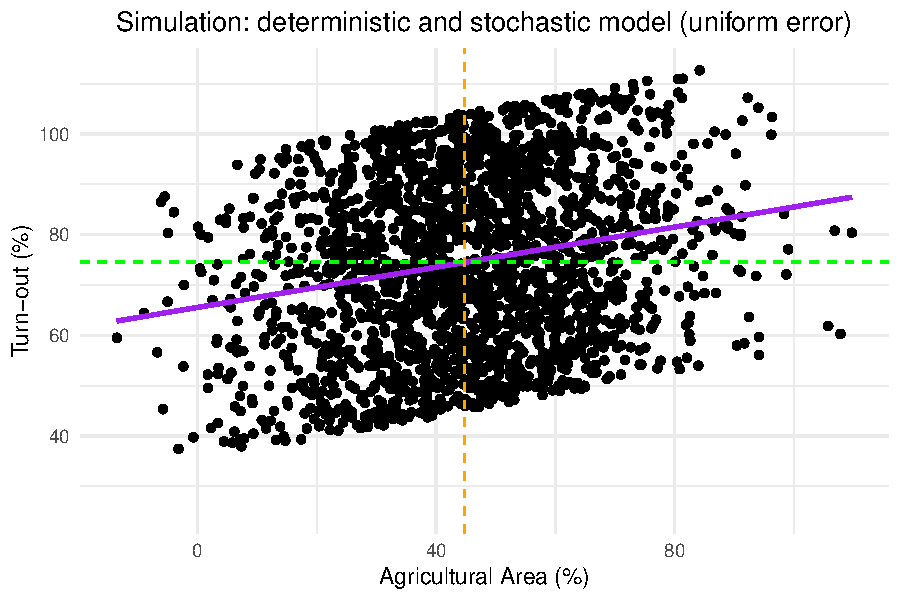
\includegraphics{_main_files/figure-latex/unnamed-chunk-58-1.pdf}

\hypertarget{appendix-getting-the-data-first}{%
\section{Appendix: Getting the data first}\label{appendix-getting-the-data-first}}

To get the data, you will use an API (application programming interface). Put plainly, for the sake of this exercise you can think of an API like a \href{https://www.youtube.com/watch?v=s7wmiS2mSXY}{waiter} to whom you make a request and who gets what ever you requested from the kitchen (a remote data source).

In this case, you will use two APIs: to get election results in Switzerland, \href{https://politanch.github.io/swissdd/index.html}{\texttt{swissdd}}, and \href{https://github.com/lgnbhl/BFS}{\texttt{BFS}} to get many other kinds of statistical information. Both APIs get information from the Federal Statistical Office (Bundesamt für Statistik).

Skimm the functions of the \href{https://politanch.github.io/swissdd/reference/index.html}{Swissdd} package. Then, inspect the \href{https://swissvotes.ch/storage/b47562b197b7725fcfa45b3e5a4abad1b4cf14cd377136f87fd4473329a51114}{codebook} to understand what for the columns and rows stand for. Do not use more than 5 minutes doing it.

To get the data, simply execute the following code. We present you with the code so, if you want, you can know how it works and you can play around with it on your own following the code's logic.

Install the \texttt{Swissdd} package

\begin{Shaded}
\begin{Highlighting}[]
\CommentTok{\#First option  {-} from CRAN. If you install it from the github repository, make sure you have the \textasciigrave{}devtools\textasciigrave{} installed in advance.}
\CommentTok{\#install.packages("swissdd")}

\CommentTok{\#Second option}
\CommentTok{\# install.packages("devtools") \# it is necessary to comment the install.packages so the book can be rendered}
\NormalTok{devtools}\SpecialCharTok{::}\FunctionTok{install\_github}\NormalTok{(}\StringTok{"politanch/swissdd"}\NormalTok{, }\AttributeTok{force =} \ConstantTok{TRUE}\NormalTok{)}
\end{Highlighting}
\end{Shaded}

\begin{verbatim}
## 
## -- R CMD build -----------------------------------------------------------------
## * checking for file ‘/private/var/folders/fg/p53z0kxs5g35bp_2wq9x5vfdsyrmgw/T/Rtmp2TRXUG/remotesc8d81ec6ad96/politanch-swissdd-04bb42c/DESCRIPTION’ ... OK
## * preparing ‘swissdd’:
## * checking DESCRIPTION meta-information ... OK
## * checking for LF line-endings in source and make files and shell scripts
## * checking for empty or unneeded directories
## * building ‘swissdd_1.1.5.tar.gz’
## Warning: invalid uid value replaced by that for user 'nobody'
## Warning: invalid gid value replaced by that for user 'nobody'
\end{verbatim}

\begin{Shaded}
\begin{Highlighting}[]
\CommentTok{\# library(swissdd)}
\end{Highlighting}
\end{Shaded}

Retrieve the \href{https://swissvotes.ch/vote/644.00}{CO2 Act} information using \texttt{get\_nationalvotes}. The vote took place in 13/06/2021.

\begin{Shaded}
\begin{Highlighting}[]
\NormalTok{CO2}\OtherTok{\textless{}{-}}\FunctionTok{get\_nationalvotes}\NormalTok{(}\AttributeTok{votedates =} \StringTok{"2021{-}06{-}13"}\NormalTok{)}
\end{Highlighting}
\end{Shaded}

As the same day of the CO2 Act vote more initiatives were voted, keep only the one we care about for this exercise. Notice that each initiative has a numerical identifier called \texttt{id}. \href{https://swissvotes.ch/vote/644.00}{Here} you can find the numerical identifier under \texttt{Vote\ Nº}. Keep in mind that, the variable \texttt{id} has the same number as in \texttt{Vote\ Nº} with an additional zero to the right.

\begin{Shaded}
\begin{Highlighting}[]
\NormalTok{CO2}\OtherTok{\textless{}{-}}\NormalTok{ CO2 }\SpecialCharTok{\%\textgreater{}\%}
  \FunctionTok{filter}\NormalTok{(id}\SpecialCharTok{==}\DecValTok{6440}\NormalTok{)}
\end{Highlighting}
\end{Shaded}

The resulting data frame contains rows representing the results for a particular vote in a particular municipality. The columns qualify that vote. Use the \texttt{colnames()} function to see the names of the columns. Keep only those that might be relevant for your analysis.

\begin{Shaded}
\begin{Highlighting}[]
\NormalTok{CO2}\OtherTok{\textless{}{-}}\NormalTok{ CO2 }\SpecialCharTok{\%\textgreater{}\%}
  \FunctionTok{select}\NormalTok{(canton\_id, canton\_name, mun\_id, mun\_name, jaStimmenInProzent, jaStimmenAbsolut, neinStimmenAbsolut, stimmbeteiligungInProzent, eingelegteStimmzettel, anzahlStimmberechtigte, gueltigeStimmen)}
\end{Highlighting}
\end{Shaded}

Finally, as you want to see the turn-out differences between municipalities with different degrees of agriculture intensity you need to get some additional data. Run the following code.

\begin{Shaded}
\begin{Highlighting}[]
\CommentTok{\# install.packages("BFS")}
\CommentTok{\# library(BFS)}
\CommentTok{\#To see the information available in German}
\CommentTok{\# catalog\_data\_de \textless{}{-} bfs\_get\_catalog\_data(language = "de")}

\CommentTok{\#To see the information available in English}
\CommentTok{\#catalog\_data\_en \textless{}{-} bfs\_get\_catalog\_data(language = "en")}

\CommentTok{\#To see the information available in German that contains a particular word in the title}
\CommentTok{\#catalog\_data\_de \textless{}{-} bfs\_get\_catalog\_data(language = "de", title="Gemeinde")}

\CommentTok{\#To get the asset number (i.e., numerical id for a data set)}
\CommentTok{\# asset\_number \textless{}{-} catalog\_data\_de \%\textgreater{}\%}
\CommentTok{\#   filter(title == "Arealstatistik: Standardnomenklatur (NOAS04) nach Bezirk und Gemeinde, in Hektaren") \%\textgreater{}\%}
\CommentTok{\#   pull(number\_asset)}

\CommentTok{\#Using that asset number, the metadata (i.e., data that describes the data set) can be accessed.}
\CommentTok{\#asset\_meta \textless{}{-} bfs\_get\_asset\_metadata(number\_asset = asset\_number)}

\CommentTok{\#From the metadata, the bfs number (i.e., a alphanumeric id for the data set) can be accessed.}
\CommentTok{\#bfs\_number \textless{}{-} asset\_meta$shop$orderNr}

\CommentTok{\#Finally, using the bfs number the data set can be accessed.}
\CommentTok{\#LandUse \textless{}{-} bfs\_get\_data(number\_bfs = bfs\_number)}

\CommentTok{\#If there is a “Too Many Requests” error message, you can follow this (https://github.com/lgnbhl/BFS\#too{-}many{-}requests{-}error{-}message) }
\CommentTok{\#or download the PX file from here https://www.bfs.admin.ch/bfs/de/home/statistiken/kataloge{-}datenbanken/daten.assetdetail.24865343.html}
\CommentTok{\#install.packages("pxR")}
\CommentTok{\# library(pxR)}
\CommentTok{\#Open data}
\NormalTok{LandUse }\OtherTok{\textless{}{-}} \FunctionTok{read.px}\NormalTok{(}\StringTok{\textquotesingle{}Data/px{-}x{-}0202020000\_102.px\textquotesingle{}}\NormalTok{, }\AttributeTok{encoding =} \StringTok{"UTF{-}8"}\NormalTok{)}
\NormalTok{LandUseData}\OtherTok{\textless{}{-}}\NormalTok{ LandUse}\SpecialCharTok{$}\NormalTok{DATA}\SpecialCharTok{$}\NormalTok{value}

\CommentTok{\#Rename variable}
\NormalTok{LandUseData }\OtherTok{\textless{}{-}}\NormalTok{ LandUseData }\SpecialCharTok{\%\textgreater{}\%}
  \FunctionTok{rename\_with}\NormalTok{(}\SpecialCharTok{\textasciitilde{}} \StringTok{\textquotesingle{}mun\_name\textquotesingle{}}\NormalTok{, }\DecValTok{3}\NormalTok{)}

\CommentTok{\#Keep the data relevant for my analysis}
\NormalTok{LandUseData}\OtherTok{\textless{}{-}}\NormalTok{ LandUseData }\SpecialCharTok{\%\textgreater{}\%}
  \FunctionTok{filter}\NormalTok{(Periode }\SpecialCharTok{==} \StringTok{"2013/18"}\NormalTok{) }\SpecialCharTok{\%\textgreater{}\%}
  \FunctionTok{filter}\NormalTok{(Standardnomenklatur..NOAS04.}\SpecialCharTok{==}\StringTok{"{-}b Landwirtschaftsflächen"} \SpecialCharTok{|}\NormalTok{ Standardnomenklatur..NOAS04.}\SpecialCharTok{==}\StringTok{"Fläche Total"}\NormalTok{) }\SpecialCharTok{\%\textgreater{}\%}
  \FunctionTok{filter}\NormalTok{(}\FunctionTok{str\_starts}\NormalTok{(}\FunctionTok{str\_trim}\NormalTok{(mun\_name), }\FunctionTok{fixed}\NormalTok{(}\StringTok{"."}\NormalTok{))) }\SpecialCharTok{\%\textgreater{}\%}
  \FunctionTok{mutate}\NormalTok{(}\AttributeTok{mun\_name =} \FunctionTok{str\_replace\_all}\NormalTok{(mun\_name, }\FunctionTok{fixed}\NormalTok{(}\StringTok{"......"}\NormalTok{), }\StringTok{""}\NormalTok{))}

\CommentTok{\# install.packages("tidyverse")}
\CommentTok{\#Adjust data from long to wide}
\NormalTok{LandUseData }\OtherTok{\textless{}{-}}\NormalTok{ LandUseData }\SpecialCharTok{\%\textgreater{}\%}
  \FunctionTok{pivot\_wider}\NormalTok{(}\AttributeTok{names\_from =}\NormalTok{ Standardnomenklatur..NOAS04., }\AttributeTok{values\_from =}\NormalTok{ value)}

\CommentTok{\#Rename variables}
\NormalTok{LandUseData }\OtherTok{\textless{}{-}}\NormalTok{ LandUseData }\SpecialCharTok{\%\textgreater{}\%}
  \FunctionTok{rename\_with}\NormalTok{(}\SpecialCharTok{\textasciitilde{}} \StringTok{\textquotesingle{}TotalAreaHa\textquotesingle{}}\NormalTok{, }\DecValTok{3}\NormalTok{) }\SpecialCharTok{\%\textgreater{}\%}
  \FunctionTok{rename\_with}\NormalTok{(}\SpecialCharTok{\textasciitilde{}} \StringTok{\textquotesingle{}AgriculturalAreaHa\textquotesingle{}}\NormalTok{, }\DecValTok{4}\NormalTok{) }\SpecialCharTok{\%\textgreater{}\%}
  \FunctionTok{select}\NormalTok{(}\SpecialCharTok{{-}}\NormalTok{Periode)}
\end{Highlighting}
\end{Shaded}

Using the additional data, you can now merge both data sets so you can know how did voters behave in more agricultural areas. Use the \texttt{inner\_join} function. The numerical IDs are available in \texttt{LandUseData} but not in \texttt{CO2}. However, as both sources share the \texttt{mun\_name}, you use that variable to match them.

\begin{Shaded}
\begin{Highlighting}[]
\NormalTok{CO2 }\OtherTok{\textless{}{-}} \FunctionTok{inner\_join}\NormalTok{(CO2, LandUseData, }\AttributeTok{by=}\StringTok{"mun\_name"}\NormalTok{)  }

\FunctionTok{write.csv}\NormalTok{(CO2, }\StringTok{"Data/CO2\_land.csv"}\NormalTok{)}
\end{Highlighting}
\end{Shaded}

\hypertarget{week-4-regression-ii-model-specification}{%
\chapter{Week 4: Regression II (Model Specification)}\label{week-4-regression-ii-model-specification}}

\hypertarget{aims-2}{%
\section{Aims}\label{aims-2}}

\begin{enumerate}
\def\labelenumi{\arabic{enumi}.}
\tightlist
\item
  Using multiple regressors and interaction terms in regression analysis for quantitative descriptive purposes with real data
\item
  Using simulation to instantiate how different properties of the data generating process alter or not metrics of goodness of fit
\end{enumerate}

\hypertarget{exercise-context-and-questions}{%
\section{Exercise: Context and questions}\label{exercise-context-and-questions}}

Currently led by \href{https://forscenter.ch/staff/anke-tresch/}{Prof.~Anke Tresch}, ``{[}t{]}he Swiss Election Study (Selects) has been investigating the electoral behaviour of Swiss citizens in national elections since 1995. The project sheds light on the dynamics of the citizens' opinion formation as well as on the determinants of their political participation and voting choice for a specific candidate or party.'' See more \href{https://forscenter.ch/projects/selects/}{here}.

In this exercise, you will use data for the year 2019. You will use it to answer the following questions:

\begin{enumerate}
\def\labelenumi{\arabic{enumi}.}
\tightlist
\item
  Do older voters have stronger right leaning preferences than younger ones?
\item
  Do political preferences vary across sexes?
\item
  Do political preferences vary across the main language spoken at the respondent's home?
\item
  Do differences in political preferences across sexes vary depending on the respondents' age?
\item
  Do differences in political preferences across sexes vary depending on the respondents' main language?
\item
  Do differences in political preferences across main languages vary depending on the respondents' age?
\item
  Do differences in political preferences across sexes vary depending on the respondents' age and main language?
\end{enumerate}

\hypertarget{adjusting-the-data-first}{%
\section{Adjusting the data first}\label{adjusting-the-data-first}}

In the folder \texttt{SELECTS\ 2019}, you can find the file \texttt{data.csv}. It is a version of the SELECTS data for 2019 only with the variables relevant for our exercise.

\begin{enumerate}
\def\labelenumi{\arabic{enumi}.}
\tightlist
\item
  Open the file:
\end{enumerate}

\begin{Shaded}
\begin{Highlighting}[]
\NormalTok{selects19 }\OtherTok{\textless{}{-}} \FunctionTok{read.csv}\NormalTok{(}\StringTok{"Data/SELECTS 2019/data.csv"}\NormalTok{, }\AttributeTok{header =} \ConstantTok{TRUE}\NormalTok{)}
\end{Highlighting}
\end{Shaded}

\begin{enumerate}
\def\labelenumi{\arabic{enumi}.}
\setcounter{enumi}{1}
\tightlist
\item
  In order to store information in smaller files, researchers use codebooks to numerically represent values that, otherwise, would be much more space consuming in their respective representation in text form. Use the file \texttt{Selects2019\_Codebook\_EN.pdf} to create the variable \texttt{LanguageHome} where the numerical values for the variable \texttt{f20221} (i.e., ``Main language spoken in family or at home'') are preplaced with their respective text values.
\end{enumerate}

\begin{Shaded}
\begin{Highlighting}[]
\NormalTok{selects19 }\OtherTok{\textless{}{-}}\NormalTok{ selects19 }\SpecialCharTok{\%\textgreater{}\%}
  \FunctionTok{mutate}\NormalTok{(}\AttributeTok{LanguageHome =} \FunctionTok{case\_when}\NormalTok{( }\CommentTok{\#a new variable is created}
\CommentTok{\#each numerical value in the codebook is replace with it\textquotesingle{}s corresponding text value}
\NormalTok{    f20221 }\SpecialCharTok{==} \DecValTok{1} \SpecialCharTok{\textasciitilde{}} \StringTok{"German/Swiss German"}\NormalTok{, }
\NormalTok{    f20221 }\SpecialCharTok{==} \DecValTok{2} \SpecialCharTok{\textasciitilde{}} \StringTok{"French"}\NormalTok{,}
\NormalTok{    f20221 }\SpecialCharTok{==} \DecValTok{3} \SpecialCharTok{\textasciitilde{}} \StringTok{"Italian"}\NormalTok{,}
\NormalTok{    f20221 }\SpecialCharTok{==} \DecValTok{4} \SpecialCharTok{\textasciitilde{}} \StringTok{"Romansh"}\NormalTok{,}
\NormalTok{    f20221 }\SpecialCharTok{==} \DecValTok{5} \SpecialCharTok{\textasciitilde{}} \StringTok{"Other"}\NormalTok{))}
\end{Highlighting}
\end{Shaded}

\begin{enumerate}
\def\labelenumi{\arabic{enumi}.}
\setcounter{enumi}{2}
\tightlist
\item
  As we have seen in week 1, it is a good practice to name your variables so their interpretation is easy. For example, instead of using \texttt{sex} as a variable name, using \texttt{female} facilitates understanding that a zero represents \texttt{male} while a one represents \texttt{female}. Again, use the codebook to transform the variable \texttt{sex} into \texttt{female}.
\end{enumerate}

Relabel the \texttt{sex} variable:

\begin{Shaded}
\begin{Highlighting}[]
\NormalTok{selects19 }\OtherTok{\textless{}{-}}\NormalTok{ selects19 }\SpecialCharTok{\%\textgreater{}\%}
  \FunctionTok{mutate}\NormalTok{(}\AttributeTok{sex =} \FunctionTok{case\_when}\NormalTok{(}
\NormalTok{    sex }\SpecialCharTok{==} \DecValTok{1} \SpecialCharTok{\textasciitilde{}} \DecValTok{0}\NormalTok{,}
\NormalTok{    sex }\SpecialCharTok{==} \DecValTok{2} \SpecialCharTok{\textasciitilde{}} \DecValTok{1}\NormalTok{))}
\end{Highlighting}
\end{Shaded}

Rename the variable \texttt{sex} as \texttt{female}. Take the chance and rename \texttt{f15200} (i.e., ``Left-right placement - Self'') as \texttt{LeftToRight}.

\begin{Shaded}
\begin{Highlighting}[]
\NormalTok{selects19 }\OtherTok{\textless{}{-}}\NormalTok{ dplyr}\SpecialCharTok{::}\FunctionTok{rename}\NormalTok{(selects19, }\AttributeTok{LeftToRight =}\NormalTok{ f15200, }\AttributeTok{female =}\NormalTok{ sex)}
\end{Highlighting}
\end{Shaded}

\begin{enumerate}
\def\labelenumi{\arabic{enumi}.}
\setcounter{enumi}{3}
\tightlist
\item
  Print the name of all the variables available so you can use them later on.
\end{enumerate}

\begin{Shaded}
\begin{Highlighting}[]
\FunctionTok{names}\NormalTok{(selects19)}
\end{Highlighting}
\end{Shaded}

\begin{verbatim}
## [1] "female"       "age"          "LeftToRight"  "f20221"       "LanguageHome"
\end{verbatim}

\hypertarget{exercise-solution-1}{%
\section{Exercise: solution}\label{exercise-solution-1}}

\textbf{Note:} Remember that you can copy the code from one point to answer another point. Simply make the necessary adjustments.

\hypertarget{real-data-1}{%
\subsection{Real data}\label{real-data-1}}

\begin{enumerate}
\def\labelenumi{\arabic{enumi}.}
\tightlist
\item
  Graph age vs.~political preferences. Use a linear regression line to describe how the variables relate to each other.
\end{enumerate}

\begin{Shaded}
\begin{Highlighting}[]
\CommentTok{\#Means for Y and X: to have a clearer notion on the center of mass of the data.}
\NormalTok{mean\_LeftRight }\OtherTok{\textless{}{-}} \FunctionTok{mean}\NormalTok{(selects19}\SpecialCharTok{$}\NormalTok{LeftToRight, }\AttributeTok{na.rm =} \ConstantTok{TRUE}\NormalTok{)}
\NormalTok{mean\_age }\OtherTok{\textless{}{-}} \FunctionTok{mean}\NormalTok{(selects19}\SpecialCharTok{$}\NormalTok{age, }\AttributeTok{na.rm =} \ConstantTok{TRUE}\NormalTok{)}

\CommentTok{\# Create a scatter plot}
\FunctionTok{ggplot}\NormalTok{(selects19, }\FunctionTok{aes}\NormalTok{(}\AttributeTok{x =}\NormalTok{ age, }\AttributeTok{y =}\NormalTok{ LeftToRight)) }\SpecialCharTok{+}
  \FunctionTok{geom\_point}\NormalTok{() }\SpecialCharTok{+}
  \CommentTok{\# Adding the regression line}
  \FunctionTok{geom\_smooth}\NormalTok{(}\AttributeTok{method =} \StringTok{"lm"}\NormalTok{, }\AttributeTok{formula =}\NormalTok{ y }\SpecialCharTok{\textasciitilde{}}\NormalTok{ x, }\AttributeTok{se =} \ConstantTok{FALSE}\NormalTok{, }\AttributeTok{color =} \StringTok{"red"}\NormalTok{) }\SpecialCharTok{+}  
  \CommentTok{\# Horizontal line at the mean of y}
  \FunctionTok{geom\_hline}\NormalTok{(}\AttributeTok{yintercept =}\NormalTok{ mean\_LeftRight, }\AttributeTok{linetype =} \StringTok{"dashed"}\NormalTok{, }\AttributeTok{color =} \StringTok{"green"}\NormalTok{) }\SpecialCharTok{+}  
  \CommentTok{\# Vertical line at the mean of x}
  \FunctionTok{geom\_vline}\NormalTok{(}\AttributeTok{xintercept =}\NormalTok{ mean\_age, }\AttributeTok{linetype =} \StringTok{"dashed"}\NormalTok{, }\AttributeTok{color =} \StringTok{"orange"}\NormalTok{) }\SpecialCharTok{+}  
  \FunctionTok{theme\_minimal}\NormalTok{() }\SpecialCharTok{+}
  \FunctionTok{theme}\NormalTok{(}\AttributeTok{plot.title =} \FunctionTok{element\_text}\NormalTok{(}\AttributeTok{hjust =} \FloatTok{0.5}\NormalTok{)) }\SpecialCharTok{+}
  \FunctionTok{labs}\NormalTok{(}
    \AttributeTok{x =} \StringTok{"Age (years)"}\NormalTok{,}
    \AttributeTok{y =} \StringTok{"Political Preferences (left to right)"}\NormalTok{,}
    \AttributeTok{title =} \StringTok{"Scatter plot Age vs. Political Preferences"}
\NormalTok{  )}
\end{Highlighting}
\end{Shaded}

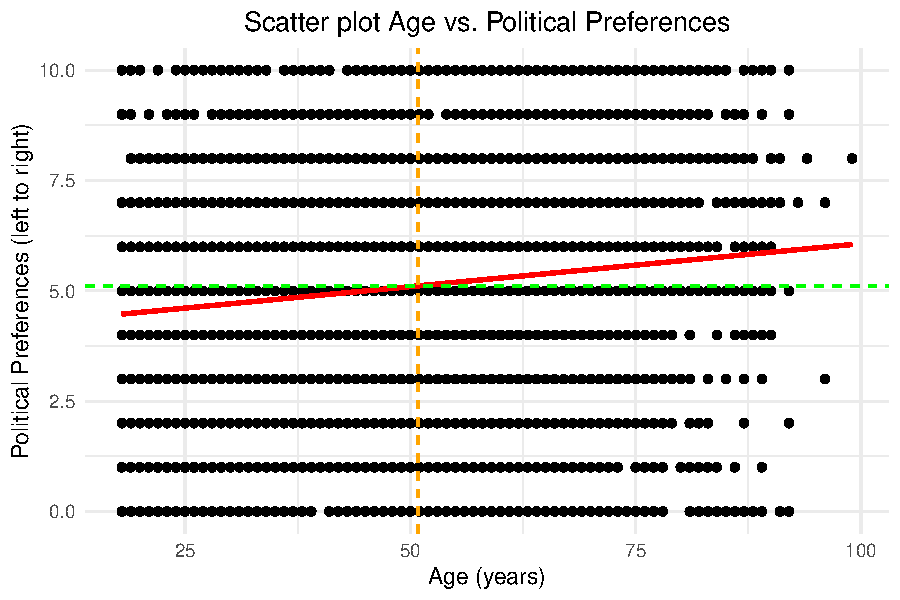
\includegraphics{_main_files/figure-latex/unnamed-chunk-72-1.pdf}

Therefore, we can say that, indeed, older voters have stronger right leaning preferences than younger ones.

\begin{enumerate}
\def\labelenumi{\arabic{enumi}.}
\setcounter{enumi}{1}
\tightlist
\item
  Since the political preferences as well as years are defined in discrete values, many values can overlap for the same pair\texttt{(preference,\ age)}. Use the \texttt{ggridges} package to see how do preferences distribute across different age values.
\end{enumerate}

\begin{Shaded}
\begin{Highlighting}[]
\FunctionTok{ggplot}\NormalTok{(selects19, }\FunctionTok{aes}\NormalTok{(}\AttributeTok{x =}\NormalTok{ age, }\AttributeTok{y =} \FunctionTok{as.factor}\NormalTok{(LeftToRight), }\AttributeTok{fill =} \FunctionTok{as.factor}\NormalTok{(LeftToRight))) }\SpecialCharTok{+}
  \CommentTok{\# to show the age distribution for each level of political preference}
  \FunctionTok{geom\_density\_ridges}\NormalTok{() }\SpecialCharTok{+} 
  \FunctionTok{geom\_smooth}\NormalTok{(}\AttributeTok{data =}\NormalTok{ selects19, }\FunctionTok{aes}\NormalTok{(}\AttributeTok{x =}\NormalTok{ age, }\AttributeTok{y =}\NormalTok{ LeftToRight, }\AttributeTok{group =} \DecValTok{1}\NormalTok{), }
              \AttributeTok{method =} \StringTok{"lm"}\NormalTok{, }\AttributeTok{formula =}\NormalTok{ y }\SpecialCharTok{\textasciitilde{}}\NormalTok{ x, }\AttributeTok{color =} \StringTok{"red"}\NormalTok{, }\AttributeTok{se =} \ConstantTok{FALSE}\NormalTok{) }\SpecialCharTok{+}
  \FunctionTok{geom\_hline}\NormalTok{(}\AttributeTok{yintercept =}\NormalTok{ mean\_LeftRight, }\AttributeTok{linetype =} \StringTok{"dashed"}\NormalTok{, }\AttributeTok{color =} \StringTok{"green"}\NormalTok{) }\SpecialCharTok{+}
  \FunctionTok{geom\_vline}\NormalTok{(}\AttributeTok{xintercept =}\NormalTok{ mean\_age, }\AttributeTok{linetype =} \StringTok{"dashed"}\NormalTok{, }\AttributeTok{color =} \StringTok{"orange"}\NormalTok{) }\SpecialCharTok{+}
  \FunctionTok{scale\_fill\_viridis\_d}\NormalTok{() }\SpecialCharTok{+}
  \FunctionTok{theme\_minimal}\NormalTok{() }\SpecialCharTok{+}
  \FunctionTok{theme}\NormalTok{(}\AttributeTok{legend.position =} \StringTok{"none"}\NormalTok{) }\SpecialCharTok{+}
  \FunctionTok{theme}\NormalTok{(}\AttributeTok{plot.title =} \FunctionTok{element\_text}\NormalTok{(}\AttributeTok{hjust =} \FloatTok{0.5}\NormalTok{)) }\SpecialCharTok{+}
  \FunctionTok{labs}\NormalTok{(}\AttributeTok{x =} \StringTok{"Age (years)"}\NormalTok{,}
       \AttributeTok{y =} \StringTok{"Political Preferences (left to right)"}\NormalTok{,}
       \AttributeTok{title =} \StringTok{"Political preferences by age level"}\NormalTok{,}
       \AttributeTok{fill =} \StringTok{"factor(LeftToRight)"}\NormalTok{)}
\end{Highlighting}
\end{Shaded}

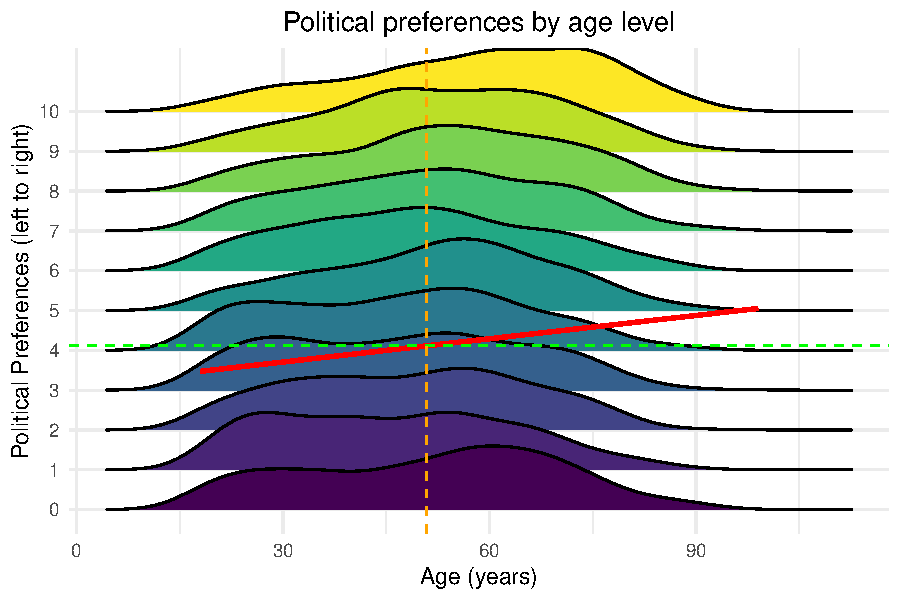
\includegraphics{_main_files/figure-latex/unnamed-chunk-73-1.pdf}

\begin{enumerate}
\def\labelenumi{\arabic{enumi}.}
\setcounter{enumi}{2}
\tightlist
\item
  Regress the political preferences on age. As we learnt in the exercises from last week, the regression with intercept fits data better in most cases: act accordingly. Report and interpret the parameters. Graph some of the main components of the regression output.
\end{enumerate}

\begin{itemize}
\tightlist
\item
  Write the regression here.
\end{itemize}

\begin{Shaded}
\begin{Highlighting}[]
\CommentTok{\#regression}
\NormalTok{result }\OtherTok{\textless{}{-}} \FunctionTok{lm}\NormalTok{(LeftToRight }\SpecialCharTok{\textasciitilde{}}\NormalTok{ age, }\AttributeTok{data =}\NormalTok{ selects19)}
\FunctionTok{summary}\NormalTok{(result)}
\end{Highlighting}
\end{Shaded}

\begin{verbatim}
## 
## Call:
## lm(formula = LeftToRight ~ age, data = selects19)
## 
## Residuals:
##     Min      1Q  Median      3Q     Max 
## -5.9150 -2.0380 -0.0186  2.1958  5.5271 
## 
## Coefficients:
##             Estimate Std. Error t value Pr(>|t|)    
## (Intercept) 4.122055   0.106375  38.750   <2e-16 ***
## age         0.019489   0.001979   9.846   <2e-16 ***
## ---
## Signif. codes:  0 '***' 0.001 '**' 0.01 '*' 0.05 '.' 0.1 ' ' 1
## 
## Residual standard error: 2.649 on 5905 degrees of freedom
## Multiple R-squared:  0.01615,    Adjusted R-squared:  0.01598 
## F-statistic: 96.94 on 1 and 5905 DF,  p-value: < 2.2e-16
\end{verbatim}

\begin{itemize}
\tightlist
\item
  Report and interpret the parameters here.
\end{itemize}

\begin{Shaded}
\begin{Highlighting}[]
\NormalTok{coeffs}\OtherTok{\textless{}{-}} \FunctionTok{coef}\NormalTok{(result)}
\NormalTok{coeffs}
\end{Highlighting}
\end{Shaded}

\begin{verbatim}
## (Intercept)         age 
##  4.12205528  0.01948902
\end{verbatim}

The beta value for (Intercept) is 4.12, and for \texttt{r}names(coeffs{[}2{]})` is 0.02.

It means that, \emph{given our model}, an increase of one year in age across the Swiss citizens is associated with an average increase in the \texttt{LeftToRight} self-declared scale of 0.02 ideological units. Likewise, , \emph{given our model}, newborns can be expected to have an average ideological value of 4.12, while 100 year old citizens can be expected to have an average ideological value of 6.12. We must, nonetheless, remain cautious and keep our predictions as much as possible within the range of regressors our sample provides us with.

\begin{itemize}
\tightlist
\item
  Graph some of the main components of the regression output here.
\end{itemize}

\begin{Shaded}
\begin{Highlighting}[]
\FunctionTok{ggplot}\NormalTok{(selects19, }\FunctionTok{aes}\NormalTok{(}\AttributeTok{x =}\NormalTok{ age, }\AttributeTok{y =}\NormalTok{ LeftToRight)) }\SpecialCharTok{+}  \CommentTok{\# Removed selects19$ from aes(), not necessary}
  \FunctionTok{geom\_point}\NormalTok{(}\AttributeTok{size =} \FloatTok{0.001}\NormalTok{) }\SpecialCharTok{+}
  \FunctionTok{geom\_abline}\NormalTok{(}\FunctionTok{aes}\NormalTok{(}\AttributeTok{intercept =} \FunctionTok{unname}\NormalTok{(coeffs[}\DecValTok{1}\NormalTok{]),}
                \AttributeTok{slope =} \DecValTok{0}\NormalTok{, }
                \AttributeTok{color =} \StringTok{"Newborn"}\NormalTok{)) }\SpecialCharTok{+}
  
  \FunctionTok{geom\_abline}\NormalTok{(}\FunctionTok{aes}\NormalTok{(}\AttributeTok{intercept =} \FunctionTok{unname}\NormalTok{(coeffs[}\DecValTok{1}\NormalTok{]),}
                \AttributeTok{slope =} \FunctionTok{unname}\NormalTok{(coeffs[}\DecValTok{2}\NormalTok{]), }
                \AttributeTok{color =} \StringTok{"Average individual over time"}\NormalTok{)) }\SpecialCharTok{+}
  
  \CommentTok{\# Define colors for the legend}
  \FunctionTok{scale\_color\_manual}\NormalTok{(}\AttributeTok{name =} \StringTok{"Lines"}\NormalTok{, }\AttributeTok{values =} \FunctionTok{c}\NormalTok{(}\StringTok{"Newborn"} \OtherTok{=} \StringTok{"gray"}\NormalTok{, }\StringTok{"Average individual over time"} \OtherTok{=} \StringTok{"red"}\NormalTok{)) }\SpecialCharTok{+}
  
  \FunctionTok{theme\_minimal}\NormalTok{() }\SpecialCharTok{+}
  \FunctionTok{theme}\NormalTok{(}\AttributeTok{plot.title =} \FunctionTok{element\_text}\NormalTok{(}\AttributeTok{hjust =} \FloatTok{0.5}\NormalTok{)) }\SpecialCharTok{+}
  \FunctionTok{labs}\NormalTok{(}
    \AttributeTok{x =} \StringTok{"Age (years)"}\NormalTok{,}
    \AttributeTok{y =} \StringTok{"Political Preferences (left to right)"}\NormalTok{,}
    \AttributeTok{title =} \StringTok{"Relationship political preferences across ages"}
\NormalTok{  )}
\end{Highlighting}
\end{Shaded}

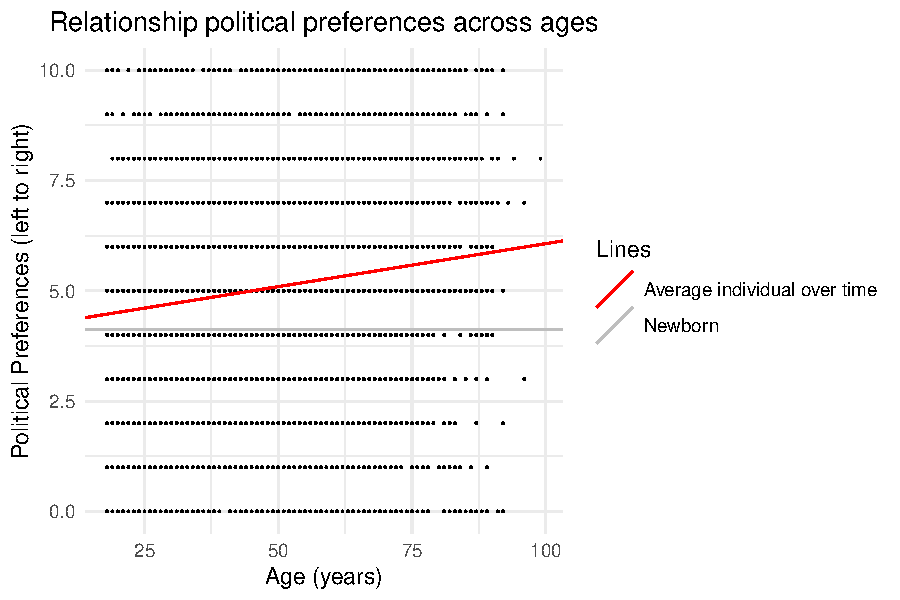
\includegraphics{_main_files/figure-latex/unnamed-chunk-76-1.pdf}

\begin{enumerate}
\def\labelenumi{\arabic{enumi}.}
\setcounter{enumi}{3}
\tightlist
\item
  Now regress \texttt{LeftToRight} on \texttt{age} and \texttt{female}. do the same as in the previous point. Report and interpret the parameters. Graph some of the main components of the regression output.
  Write the regression here.
\end{enumerate}

\begin{Shaded}
\begin{Highlighting}[]
\CommentTok{\#regression}
\NormalTok{result }\OtherTok{\textless{}{-}} \FunctionTok{lm}\NormalTok{(LeftToRight }\SpecialCharTok{\textasciitilde{}}\NormalTok{ age }\SpecialCharTok{+}\NormalTok{ female, }\AttributeTok{data =}\NormalTok{ selects19)}
\FunctionTok{summary}\NormalTok{(result)}
\end{Highlighting}
\end{Shaded}

\begin{verbatim}
## 
## Call:
## lm(formula = LeftToRight ~ age + female, data = selects19)
## 
## Residuals:
##     Min      1Q  Median      3Q     Max 
## -6.2108 -1.9784  0.0954  2.1145  5.8236 
## 
## Coefficients:
##              Estimate Std. Error t value Pr(>|t|)    
## (Intercept)  4.492964   0.112519  39.931   <2e-16 ***
## age          0.018672   0.001966   9.496   <2e-16 ***
## female      -0.652678   0.068477  -9.531   <2e-16 ***
## ---
## Signif. codes:  0 '***' 0.001 '**' 0.01 '*' 0.05 '.' 0.1 ' ' 1
## 
## Residual standard error: 2.629 on 5904 degrees of freedom
## Multiple R-squared:  0.03106,    Adjusted R-squared:  0.03073 
## F-statistic: 94.63 on 2 and 5904 DF,  p-value: < 2.2e-16
\end{verbatim}

Report and interpret the parameters here.

\begin{Shaded}
\begin{Highlighting}[]
\NormalTok{coeffs}\OtherTok{\textless{}{-}} \FunctionTok{coef}\NormalTok{(result)}
\NormalTok{coeffs}
\end{Highlighting}
\end{Shaded}

\begin{verbatim}
## (Intercept)         age      female 
##  4.49296422  0.01867214 -0.65267756
\end{verbatim}

The beta value for (Intercept), ' is 4.49, for age, is 0.02, and for female is -0.65.

It means that, given our model, an increase of one year in age across the Swiss citizens is associated with an average increase in the LeftToRight self-declared scale of 0.02, \emph{ideological units}. Likewise, male newborns can be expected to have an average ideological value of 4.49, while 100 year old male citizens can be expected to have an average ideological value of 6.49. Similarly, for each of those scenarios, should the individual be a female, it can be expected to have an average of 0.65 ideological units lower than a male individual under the same statistical circumstances. In other words, by design, our particular model only captures the average evolution of ideology over time but does not distinguish whether nor how it varies across sexes. Finally, just as in the previous point, we must remain cautious and keep our predictions as much as possible within the range of regressors our sample provides us with.

\begin{itemize}
\tightlist
\item
  Graph some of the main components of the regression output here.
\end{itemize}

\begin{Shaded}
\begin{Highlighting}[]
\FunctionTok{ggplot}\NormalTok{(selects19, }\FunctionTok{aes}\NormalTok{(}\AttributeTok{x =}\NormalTok{ age, }\AttributeTok{y =}\NormalTok{ LeftToRight)) }\SpecialCharTok{+} 
  \FunctionTok{geom\_point}\NormalTok{(}\AttributeTok{size =} \FloatTok{0.001}\NormalTok{) }\SpecialCharTok{+}
  \FunctionTok{geom\_abline}\NormalTok{(}\FunctionTok{aes}\NormalTok{(}\AttributeTok{intercept =} \FunctionTok{unname}\NormalTok{(coeffs[}\DecValTok{1}\NormalTok{]), }\AttributeTok{slope =} \DecValTok{0}\NormalTok{, }\AttributeTok{color =} \StringTok{"Male newborn"}\NormalTok{)) }\SpecialCharTok{+}
  \FunctionTok{geom\_abline}\NormalTok{(}\FunctionTok{aes}\NormalTok{(}\AttributeTok{intercept =} \FunctionTok{unname}\NormalTok{(coeffs[}\DecValTok{1}\NormalTok{]) }\SpecialCharTok{+} \FunctionTok{unname}\NormalTok{(coeffs[}\DecValTok{3}\NormalTok{]), }\AttributeTok{slope =} \DecValTok{0}\NormalTok{, }\AttributeTok{color =} \StringTok{"Female newborn"}\NormalTok{)) }\SpecialCharTok{+}
  \FunctionTok{geom\_abline}\NormalTok{(}\FunctionTok{aes}\NormalTok{(}\AttributeTok{intercept =} \FunctionTok{unname}\NormalTok{(coeffs[}\DecValTok{1}\NormalTok{]), }\AttributeTok{slope =} \FunctionTok{unname}\NormalTok{(coeffs[}\DecValTok{2}\NormalTok{]), }\AttributeTok{color =} \StringTok{"Male over time"}\NormalTok{)) }\SpecialCharTok{+}
  \FunctionTok{geom\_abline}\NormalTok{(}\FunctionTok{aes}\NormalTok{(}\AttributeTok{intercept =} \FunctionTok{unname}\NormalTok{(coeffs[}\DecValTok{1}\NormalTok{]) }\SpecialCharTok{+} \FunctionTok{unname}\NormalTok{(coeffs[}\DecValTok{3}\NormalTok{]), }\AttributeTok{slope =} \FunctionTok{unname}\NormalTok{(coeffs[}\DecValTok{2}\NormalTok{]), }\AttributeTok{color =} \StringTok{"Female over time"}\NormalTok{)) }\SpecialCharTok{+}
  \FunctionTok{scale\_color\_manual}\NormalTok{(}\AttributeTok{name =} \StringTok{"Lines"}\NormalTok{, }\AttributeTok{values =} \FunctionTok{c}\NormalTok{(}\StringTok{"Male newborn"} \OtherTok{=} \StringTok{"gray"}\NormalTok{, }\StringTok{"Female newborn"} \OtherTok{=} \StringTok{"red"}\NormalTok{, }\StringTok{"Male over time"} \OtherTok{=} \StringTok{"orange"}\NormalTok{, }\StringTok{"Female over time"} \OtherTok{=} \StringTok{"purple"}\NormalTok{)) }\SpecialCharTok{+}
  \FunctionTok{theme\_minimal}\NormalTok{() }\SpecialCharTok{+}
  \FunctionTok{theme}\NormalTok{(}\AttributeTok{plot.title =} \FunctionTok{element\_text}\NormalTok{(}\AttributeTok{hjust =} \FloatTok{0.5}\NormalTok{)) }\SpecialCharTok{+}

  \FunctionTok{labs}\NormalTok{(}
    \AttributeTok{x =} \StringTok{"Age (years)"}\NormalTok{,}
    \AttributeTok{y =} \StringTok{"Political Preferences (left to right)"}\NormalTok{,}
    \AttributeTok{title =} \StringTok{"Relationship political preferences across ages by sex }\SpecialCharTok{\textbackslash{}n}\StringTok{(without interaction)"}\NormalTok{,}
    \AttributeTok{color =} \StringTok{"Line Type"}
\NormalTok{  )}
\end{Highlighting}
\end{Shaded}

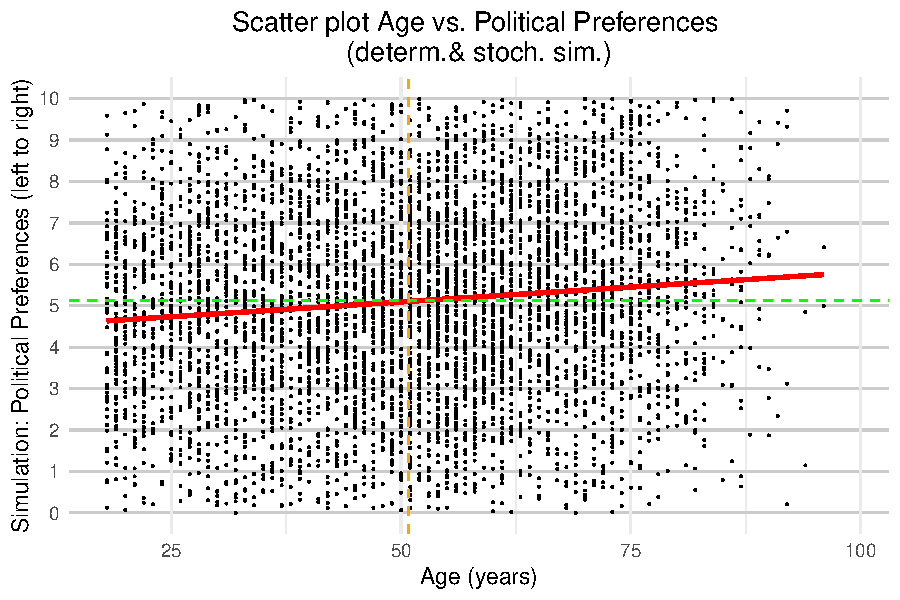
\includegraphics{_main_files/figure-latex/unnamed-chunk-79-1.pdf}

\begin{enumerate}
\def\labelenumi{\arabic{enumi}.}
\setcounter{enumi}{4}
\tightlist
\item
  You now remember that average political preferences across age can change across sexes: i.e., the average preferences across individuals in a same sex can change at different rates over time as well as begin from different departure points. Add the interaction \texttt{Age} and \texttt{female} and do the same as in the previous point.
\end{enumerate}

Write the regression here.

\begin{Shaded}
\begin{Highlighting}[]
\CommentTok{\#regression}
\NormalTok{result }\OtherTok{\textless{}{-}} \FunctionTok{lm}\NormalTok{(LeftToRight }\SpecialCharTok{\textasciitilde{}}\NormalTok{ age }\SpecialCharTok{*}\NormalTok{ female, }\AttributeTok{data =}\NormalTok{ selects19)}
\FunctionTok{summary}\NormalTok{(result)}
\end{Highlighting}
\end{Shaded}

\begin{verbatim}
## 
## Call:
## lm(formula = LeftToRight ~ age * female, data = selects19)
## 
## Residuals:
##     Min      1Q  Median      3Q     Max 
## -5.9332 -2.0641  0.0372  2.1848  6.0372 
## 
## Coefficients:
##              Estimate Std. Error t value Pr(>|t|)    
## (Intercept)  4.847656   0.152489  31.790  < 2e-16 ***
## age          0.011799   0.002801   4.213 2.56e-05 ***
## female      -1.340734   0.211254  -6.347 2.37e-10 ***
## age:female   0.013528   0.003930   3.443  0.00058 ***
## ---
## Signif. codes:  0 '***' 0.001 '**' 0.01 '*' 0.05 '.' 0.1 ' ' 1
## 
## Residual standard error: 2.626 on 5903 degrees of freedom
## Multiple R-squared:  0.033,  Adjusted R-squared:  0.03251 
## F-statistic: 67.15 on 3 and 5903 DF,  p-value: < 2.2e-16
\end{verbatim}

Report and interpret the parameters here.

\begin{Shaded}
\begin{Highlighting}[]
\NormalTok{coeffs}\OtherTok{\textless{}{-}} \FunctionTok{coef}\NormalTok{(result)}
\NormalTok{coeffs}
\end{Highlighting}
\end{Shaded}

\begin{verbatim}
## (Intercept)         age      female  age:female 
##  4.84765642  0.01179933 -1.34073442  0.01352810
\end{verbatim}

The beta value for (Intercept) is 4.85 for age is 0.01 for female is -1.34 and for age:female is 0.01.

It means that, \emph{given our model}, an increase of one year in age across the male Swiss citizens is associated with an average increase in the LeftToRight self-declared scale of 0.01 ideological units. Likewise, while male newborns can be expected to have an average ideological value of 4.85, female newborns can be expected to have an average ideological value of 3.51. Also, while 100 year old male citizens can be expected to have an average ideological value of 5.85, 100 year old females can be expected to have an average ideological value of 5.51.

Finally, while, \emph{given our model}, females have lower initial ideological initial values, the rate at which right leaning preferences increase among them over time is 0.01 ideological units per year higher than in males. Therefore, we can expect males' and females' average ideological values to converge when they are around 100 years old. Finally, just as in the previous point, we must remain cautious and keep our predictions as much as possible within the range of regressors our sample provides us with.

\begin{itemize}
\tightlist
\item
  Graph some of the main components of the regression output here.
\end{itemize}

\begin{Shaded}
\begin{Highlighting}[]
\FunctionTok{ggplot}\NormalTok{(selects19, }\FunctionTok{aes}\NormalTok{(}\AttributeTok{x =}\NormalTok{ age, }\AttributeTok{y =}\NormalTok{ LeftToRight)) }\SpecialCharTok{+} 
  \FunctionTok{geom\_point}\NormalTok{(}\AttributeTok{size =} \FloatTok{0.001}\NormalTok{) }\SpecialCharTok{+}
  \FunctionTok{geom\_abline}\NormalTok{(}\FunctionTok{aes}\NormalTok{(}\AttributeTok{intercept =} \FunctionTok{unname}\NormalTok{(coeffs[}\DecValTok{1}\NormalTok{]), }\AttributeTok{slope =} \DecValTok{0}\NormalTok{, }\AttributeTok{color =} \StringTok{"Male newborn"}\NormalTok{)) }\SpecialCharTok{+}
  \FunctionTok{geom\_abline}\NormalTok{(}\FunctionTok{aes}\NormalTok{(}\AttributeTok{intercept =} \FunctionTok{unname}\NormalTok{(coeffs[}\DecValTok{1}\NormalTok{]) }\SpecialCharTok{+} \FunctionTok{unname}\NormalTok{(coeffs[}\DecValTok{3}\NormalTok{]), }\AttributeTok{slope =} \DecValTok{0}\NormalTok{, }\AttributeTok{color =} \StringTok{"Female newborn"}\NormalTok{)) }\SpecialCharTok{+}
  \FunctionTok{geom\_abline}\NormalTok{(}\FunctionTok{aes}\NormalTok{(}\AttributeTok{intercept =} \FunctionTok{unname}\NormalTok{(coeffs[}\DecValTok{1}\NormalTok{]), }\AttributeTok{slope =} \FunctionTok{unname}\NormalTok{(coeffs[}\DecValTok{2}\NormalTok{]), }\AttributeTok{color =} \StringTok{"Male over time"}\NormalTok{)) }\SpecialCharTok{+}
  \FunctionTok{geom\_abline}\NormalTok{(}\FunctionTok{aes}\NormalTok{(}\AttributeTok{intercept =} \FunctionTok{unname}\NormalTok{(coeffs[}\DecValTok{1}\NormalTok{]) }\SpecialCharTok{+} \FunctionTok{unname}\NormalTok{(coeffs[}\DecValTok{3}\NormalTok{]), }\AttributeTok{slope =} \FunctionTok{unname}\NormalTok{(coeffs[}\DecValTok{2}\NormalTok{])}\SpecialCharTok{+}\FunctionTok{unname}\NormalTok{(coeffs[}\DecValTok{4}\NormalTok{]), }\AttributeTok{color =} \StringTok{"Female over time"}\NormalTok{)) }\SpecialCharTok{+}
  \FunctionTok{scale\_color\_manual}\NormalTok{(}\AttributeTok{name =} \StringTok{"Lines"}\NormalTok{, }\AttributeTok{values =} \FunctionTok{c}\NormalTok{(}\StringTok{"Male newborn"} \OtherTok{=} \StringTok{"gray"}\NormalTok{, }\StringTok{"Female newborn"} \OtherTok{=} \StringTok{"red"}\NormalTok{, }\StringTok{"Male over time"} \OtherTok{=} \StringTok{"orange"}\NormalTok{, }\StringTok{"Female over time"} \OtherTok{=} \StringTok{"purple"}\NormalTok{)) }\SpecialCharTok{+}
  \FunctionTok{theme\_minimal}\NormalTok{() }\SpecialCharTok{+}
  \FunctionTok{theme}\NormalTok{(}\AttributeTok{plot.title =} \FunctionTok{element\_text}\NormalTok{(}\AttributeTok{hjust =} \FloatTok{0.5}\NormalTok{)) }\SpecialCharTok{+}
  \FunctionTok{labs}\NormalTok{(}
    \AttributeTok{x =} \StringTok{"Age (years)"}\NormalTok{,}
    \AttributeTok{y =} \StringTok{"Political Preferences (left to right)"}\NormalTok{,}
    \AttributeTok{title =} \StringTok{"Relationship political preferences across ages by sex }\SpecialCharTok{\textbackslash{}n}\StringTok{(with interaction)"}
\NormalTok{  )}
\end{Highlighting}
\end{Shaded}

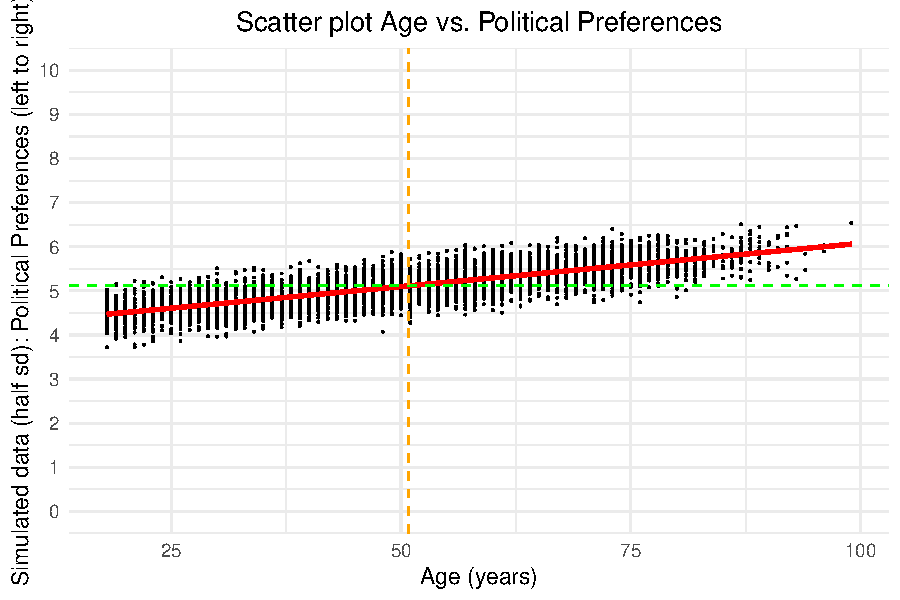
\includegraphics{_main_files/figure-latex/unnamed-chunk-82-1.pdf}

Unlike the previous point, in this point our model did not presume that the rate at which right leaning preferences increase among them over time is shared between males and females. Indeed, what the model shows is that both the intercepts and slopes are different for both groups. Particularly, \emph{give our model}, the particular mix of intercepts and slopes allow females and males to converge on their average ideological values over time.

\begin{enumerate}
\def\labelenumi{\arabic{enumi}.}
\setcounter{enumi}{5}
\tightlist
\item
  Following the same logic as in the previous point, you now add the \texttt{LanguageHome} categorical variable with the corresponding interactions. Do the same as in the previous point.
\end{enumerate}

Write the regression here.

\begin{Shaded}
\begin{Highlighting}[]
\CommentTok{\#regression}
\NormalTok{result }\OtherTok{\textless{}{-}} \FunctionTok{lm}\NormalTok{(LeftToRight }\SpecialCharTok{\textasciitilde{}}\NormalTok{ age }\SpecialCharTok{*}\NormalTok{ female }\SpecialCharTok{*}\NormalTok{ LanguageHome, }\AttributeTok{data =}\NormalTok{ selects19)}
\FunctionTok{summary}\NormalTok{(result)}
\end{Highlighting}
\end{Shaded}

\begin{verbatim}
## 
## Call:
## lm(formula = LeftToRight ~ age * female * LanguageHome, data = selects19)
## 
## Residuals:
##     Min      1Q  Median      3Q     Max 
## -6.1650 -2.0129  0.0157  2.0714  6.1504 
## 
## Coefficients:
##                                              Estimate Std. Error t value
## (Intercept)                                 4.6522028  0.2598442  17.904
## age                                         0.0092259  0.0048428   1.905
## female                                     -1.2217711  0.3489102  -3.502
## LanguageHomeGerman/Swiss German             0.1982265  0.3407428   0.582
## LanguageHomeItalian                         0.8741812  0.4954660   1.764
## LanguageHomeOther                           0.5409228  0.7585873   0.713
## LanguageHomeRomansh                        -1.2787995  2.0100116  -0.636
## age:female                                  0.0140639  0.0065181   2.158
## age:LanguageHomeGerman/Swiss German         0.0055441  0.0062621   0.885
## age:LanguageHomeItalian                    -0.0030304  0.0092982  -0.326
## age:LanguageHomeOther                      -0.0095835  0.0145811  -0.657
## age:LanguageHomeRomansh                     0.0466591  0.0397951   1.172
## female:LanguageHomeGerman/Swiss German     -0.1885585  0.4684575  -0.403
## female:LanguageHomeItalian                  0.5629460  0.7043389   0.799
## female:LanguageHomeOther                   -1.6468317  0.9783983  -1.683
## female:LanguageHomeRomansh                 -1.0259620  4.0396347  -0.254
## age:female:LanguageHomeGerman/Swiss German -0.0002337  0.0086831  -0.027
## age:female:LanguageHomeItalian             -0.0124492  0.0133246  -0.934
## age:female:LanguageHomeOther                0.0265266  0.0193016   1.374
## age:female:LanguageHomeRomansh             -0.0041536  0.0833735  -0.050
##                                            Pr(>|t|)    
## (Intercept)                                 < 2e-16 ***
## age                                        0.056817 .  
## female                                     0.000466 ***
## LanguageHomeGerman/Swiss German            0.560759    
## LanguageHomeItalian                        0.077723 .  
## LanguageHomeOther                          0.475833    
## LanguageHomeRomansh                        0.524661    
## age:female                                 0.030994 *  
## age:LanguageHomeGerman/Swiss German        0.376011    
## age:LanguageHomeItalian                    0.744501    
## age:LanguageHomeOther                      0.511041    
## age:LanguageHomeRomansh                    0.241051    
## female:LanguageHomeGerman/Swiss German     0.687324    
## female:LanguageHomeItalian                 0.424175    
## female:LanguageHomeOther                   0.092391 .  
## female:LanguageHomeRomansh                 0.799525    
## age:female:LanguageHomeGerman/Swiss German 0.978527    
## age:female:LanguageHomeItalian             0.350189    
## age:female:LanguageHomeOther               0.169395    
## age:female:LanguageHomeRomansh             0.960268    
## ---
## Signif. codes:  0 '***' 0.001 '**' 0.01 '*' 0.05 '.' 0.1 ' ' 1
## 
## Residual standard error: 2.615 on 5887 degrees of freedom
## Multiple R-squared:  0.04377,    Adjusted R-squared:  0.04068 
## F-statistic: 14.18 on 19 and 5887 DF,  p-value: < 2.2e-16
\end{verbatim}

Report and interpret the parameters here.

\begin{Shaded}
\begin{Highlighting}[]
\NormalTok{coeffs }\OtherTok{\textless{}{-}} \FunctionTok{coef}\NormalTok{(result)}
\NormalTok{coeffs}
\end{Highlighting}
\end{Shaded}

\begin{verbatim}
##                                (Intercept) 
##                               4.6522027670 
##                                        age 
##                               0.0092259369 
##                                     female 
##                              -1.2217710646 
##            LanguageHomeGerman/Swiss German 
##                               0.1982265191 
##                        LanguageHomeItalian 
##                               0.8741812107 
##                          LanguageHomeOther 
##                               0.5409227964 
##                        LanguageHomeRomansh 
##                              -1.2787994823 
##                                 age:female 
##                               0.0140639403 
##        age:LanguageHomeGerman/Swiss German 
##                               0.0055440902 
##                    age:LanguageHomeItalian 
##                              -0.0030304217 
##                      age:LanguageHomeOther 
##                              -0.0095835495 
##                    age:LanguageHomeRomansh 
##                               0.0466590996 
##     female:LanguageHomeGerman/Swiss German 
##                              -0.1885585461 
##                 female:LanguageHomeItalian 
##                               0.5629459596 
##                   female:LanguageHomeOther 
##                              -1.6468317018 
##                 female:LanguageHomeRomansh 
##                              -1.0259619787 
## age:female:LanguageHomeGerman/Swiss German 
##                              -0.0002337215 
##             age:female:LanguageHomeItalian 
##                              -0.0124491713 
##               age:female:LanguageHomeOther 
##                               0.0265265501 
##             age:female:LanguageHomeRomansh 
##                              -0.0041536238
\end{verbatim}

Interpreting a regression with ever more interactions is \textbf{exponentially harder!} The reason is that the potential scenarios to evaluate must take into account the interaction between the categorical variables of sex (i.e., two potential values) and language (i.e., five potential values) as well as the continuous variable age. In our simplest model with no interaction in point 3 we had only two parameters, in point 4 we had three, in point 5 we had four parameters with one interaction. However, in point 6 we have \emph{20} parameters. Consequently, below we present only some few cases aimed at signaling the general logic in the interpretation: we compare the male and female cases between French and Swiss German individuals.

First of all, the reference group are male newborns in French speaking households. For them, \emph{given our model}, we can expect the average political preference to be 4.65. In contrast, male newborns in Swiss German speaking households can be expected to have 0.2 ideological units more than the reference group, i.e., 4.85. Female newborns in French speaking households can be expected to have -1.22 ideological units less than the reference group, i.e., 3.43. On the other hand, Female newborns in Swiss German speaking households can be expected to have -0.19 ideological units less than the reference group, i.e., 4.46.

Likewise, for 100 year old males from French speaking households, we can expect their average political preference value to be 5.57. On the contrary, 100 year old males from Swiss German speaking households can be expected to have 0.75 ideological units more than the reference group, i.e., 6.33. In the case of 100 year old females from French speaking households, we can expect their average political preference value to be 5.76, while for 100 year old females from Swiss German speaking households we can expect their average political preference value to be 5.75.

\begin{itemize}
\tightlist
\item
  Graph some of the main components of the regression output here.
\end{itemize}

\begin{Shaded}
\begin{Highlighting}[]
\FunctionTok{ggplot}\NormalTok{(selects19, }\FunctionTok{aes}\NormalTok{(}\AttributeTok{x =}\NormalTok{ age, }\AttributeTok{y =}\NormalTok{ LeftToRight)) }\SpecialCharTok{+}
  \FunctionTok{geom\_point}\NormalTok{(}\AttributeTok{size =} \FloatTok{0.001}\NormalTok{) }\SpecialCharTok{+}
  \FunctionTok{geom\_abline}\NormalTok{(}\FunctionTok{aes}\NormalTok{(}\AttributeTok{intercept =} \FunctionTok{unname}\NormalTok{(coeffs[}\DecValTok{1}\NormalTok{]), }\AttributeTok{slope =} \DecValTok{0}\NormalTok{, }\AttributeTok{color =} \StringTok{"Male newborn French"}\NormalTok{), }\AttributeTok{linetype =} \StringTok{"dashed"}\NormalTok{) }\SpecialCharTok{+}
  \FunctionTok{geom\_abline}\NormalTok{(}\FunctionTok{aes}\NormalTok{(}\AttributeTok{intercept =} \FunctionTok{unname}\NormalTok{(coeffs[}\DecValTok{1}\NormalTok{]), }\AttributeTok{slope =} \FunctionTok{unname}\NormalTok{(coeffs[}\DecValTok{2}\NormalTok{]), }\AttributeTok{color =} \StringTok{"Male over time French"}\NormalTok{)) }\SpecialCharTok{+}

  \FunctionTok{geom\_abline}\NormalTok{(}\FunctionTok{aes}\NormalTok{(}\AttributeTok{intercept =} \FunctionTok{unname}\NormalTok{(coeffs[}\DecValTok{1}\NormalTok{]) }\SpecialCharTok{+} \FunctionTok{unname}\NormalTok{(coeffs[}\DecValTok{4}\NormalTok{]), }\AttributeTok{slope =} \DecValTok{0}\NormalTok{, }\AttributeTok{color =} \StringTok{"Male newborn Swiss German"}\NormalTok{), }\AttributeTok{linetype =} \StringTok{"dashed"}\NormalTok{) }\SpecialCharTok{+}
  \FunctionTok{geom\_abline}\NormalTok{(}\FunctionTok{aes}\NormalTok{(}\AttributeTok{intercept =} \FunctionTok{unname}\NormalTok{(coeffs[}\DecValTok{1}\NormalTok{]) }\SpecialCharTok{+} \FunctionTok{unname}\NormalTok{(coeffs[}\DecValTok{4}\NormalTok{]), }\AttributeTok{slope =} \FunctionTok{unname}\NormalTok{(coeffs[}\DecValTok{2}\NormalTok{]) }\SpecialCharTok{+} \FunctionTok{unname}\NormalTok{(coeffs[}\DecValTok{9}\NormalTok{]), }\AttributeTok{color =} \StringTok{"Male over time Swiss German"}\NormalTok{)) }\SpecialCharTok{+}

  \FunctionTok{geom\_abline}\NormalTok{(}\FunctionTok{aes}\NormalTok{(}\AttributeTok{intercept =} \FunctionTok{unname}\NormalTok{(coeffs[}\DecValTok{1}\NormalTok{]) }\SpecialCharTok{+} \FunctionTok{unname}\NormalTok{(coeffs[}\DecValTok{3}\NormalTok{]), }\AttributeTok{slope =} \DecValTok{0}\NormalTok{, }\AttributeTok{color =} \StringTok{"Female newborn French"}\NormalTok{), }\AttributeTok{size =} \DecValTok{2}\NormalTok{, }\AttributeTok{linetype =} \StringTok{"dashed"}\NormalTok{) }\SpecialCharTok{+}
  \FunctionTok{geom\_abline}\NormalTok{(}\FunctionTok{aes}\NormalTok{(}\AttributeTok{intercept =} \FunctionTok{unname}\NormalTok{(coeffs[}\DecValTok{1}\NormalTok{]) }\SpecialCharTok{+} \FunctionTok{unname}\NormalTok{(coeffs[}\DecValTok{3}\NormalTok{]), }\AttributeTok{slope =} \FunctionTok{unname}\NormalTok{(coeffs[}\DecValTok{2}\NormalTok{]) }\SpecialCharTok{+} \FunctionTok{unname}\NormalTok{(coeffs[}\DecValTok{8}\NormalTok{]), }\AttributeTok{color =} \StringTok{"Female over time French"}\NormalTok{), }\AttributeTok{size =} \DecValTok{2}\NormalTok{) }\SpecialCharTok{+}
  
  \FunctionTok{geom\_abline}\NormalTok{(}\FunctionTok{aes}\NormalTok{(}\AttributeTok{intercept =} \FunctionTok{unname}\NormalTok{(coeffs[}\DecValTok{1}\NormalTok{]) }\SpecialCharTok{+} \FunctionTok{unname}\NormalTok{(coeffs[}\DecValTok{3}\NormalTok{]) }\SpecialCharTok{+} \FunctionTok{unname}\NormalTok{(coeffs[}\DecValTok{4}\NormalTok{]) }\SpecialCharTok{+} \FunctionTok{unname}\NormalTok{(coeffs[}\DecValTok{13}\NormalTok{]),}
                  \AttributeTok{slope =} \DecValTok{0}\NormalTok{, }\AttributeTok{color =} \StringTok{"Female newborn Swiss German"}\NormalTok{), }\AttributeTok{linetype =} \StringTok{"dashed"}\NormalTok{) }\SpecialCharTok{+}
  \FunctionTok{geom\_abline}\NormalTok{(}\FunctionTok{aes}\NormalTok{(}\AttributeTok{intercept =} \FunctionTok{unname}\NormalTok{(coeffs[}\DecValTok{1}\NormalTok{]) }\SpecialCharTok{+} \FunctionTok{unname}\NormalTok{(coeffs[}\DecValTok{3}\NormalTok{]) }\SpecialCharTok{+} \FunctionTok{unname}\NormalTok{(coeffs[}\DecValTok{4}\NormalTok{]) }\SpecialCharTok{+} \FunctionTok{unname}\NormalTok{(coeffs[}\DecValTok{13}\NormalTok{]),}
                  \AttributeTok{slope =} \FunctionTok{unname}\NormalTok{(coeffs[}\DecValTok{2}\NormalTok{]) }\SpecialCharTok{+} \FunctionTok{unname}\NormalTok{(coeffs[}\DecValTok{8}\NormalTok{]) }\SpecialCharTok{+} \FunctionTok{unname}\NormalTok{(coeffs[}\DecValTok{17}\NormalTok{]), }\AttributeTok{color =} \StringTok{"Female over time Swiss German"}\NormalTok{)) }\SpecialCharTok{+}
  
  \FunctionTok{scale\_color\_manual}\NormalTok{(}\AttributeTok{name =} \StringTok{"Lines"}\NormalTok{, }\AttributeTok{values =} \FunctionTok{c}\NormalTok{(}\StringTok{"Male newborn French"} \OtherTok{=} \StringTok{"blue"}\NormalTok{, }\StringTok{"Male over time French"} \OtherTok{=} \StringTok{"blue"}\NormalTok{, }\StringTok{"Male newborn Swiss German"} \OtherTok{=} \StringTok{"red"}\NormalTok{, }\StringTok{"Male over time Swiss German"} \OtherTok{=} \StringTok{"red"}\NormalTok{, }\StringTok{"Female newborn French"} \OtherTok{=} \StringTok{"orange"}\NormalTok{, }\StringTok{"Female over time French"} \OtherTok{=} \StringTok{"orange"}\NormalTok{, }\StringTok{"Female newborn Swiss German"}\OtherTok{=} \StringTok{"purple"}\NormalTok{, }\StringTok{"Female over time Swiss German"}\OtherTok{=} \StringTok{"purple"}\NormalTok{)) }\SpecialCharTok{+}

  \FunctionTok{scale\_linetype\_manual}\NormalTok{(}\AttributeTok{name =} \StringTok{"Lines"}\NormalTok{, }\AttributeTok{values =} \FunctionTok{c}\NormalTok{(}\StringTok{"Male newborn French"} \OtherTok{=} \StringTok{"dashed"}\NormalTok{, }\StringTok{"Male over time French"} \OtherTok{=} \StringTok{"solid"}\NormalTok{, }\StringTok{"Male newborn Swiss German"} \OtherTok{=} \StringTok{"dashed"}\NormalTok{, }\StringTok{"Male over time Swiss German"} \OtherTok{=} \StringTok{"solid"}\NormalTok{, }\StringTok{"Female newborn French"} \OtherTok{=} \StringTok{"dashed"}\NormalTok{, }\StringTok{"Female over time French"} \OtherTok{=} \StringTok{"solid"}\NormalTok{, }\StringTok{"Female newborn Swiss German"} \OtherTok{=} \StringTok{"dashed"}\NormalTok{, }\StringTok{"Female over time Swiss German"} \OtherTok{=} \StringTok{"solid"}\NormalTok{)) }\SpecialCharTok{+}

  
  \FunctionTok{theme\_minimal}\NormalTok{() }\SpecialCharTok{+}
  \FunctionTok{theme}\NormalTok{(}\AttributeTok{plot.title =} \FunctionTok{element\_text}\NormalTok{(}\AttributeTok{hjust =} \FloatTok{0.5}\NormalTok{)) }\SpecialCharTok{+}
  \FunctionTok{labs}\NormalTok{(}
    \AttributeTok{x =} \StringTok{"Age (years)"}\NormalTok{,}
    \AttributeTok{y =} \StringTok{"Political Preferences (left to right)"}\NormalTok{,}
    \AttributeTok{title =} \StringTok{"Relationship political preferences across ages by sex and language }\SpecialCharTok{\textbackslash{}n}\StringTok{(with interaction)"}
\NormalTok{  )}
\end{Highlighting}
\end{Shaded}

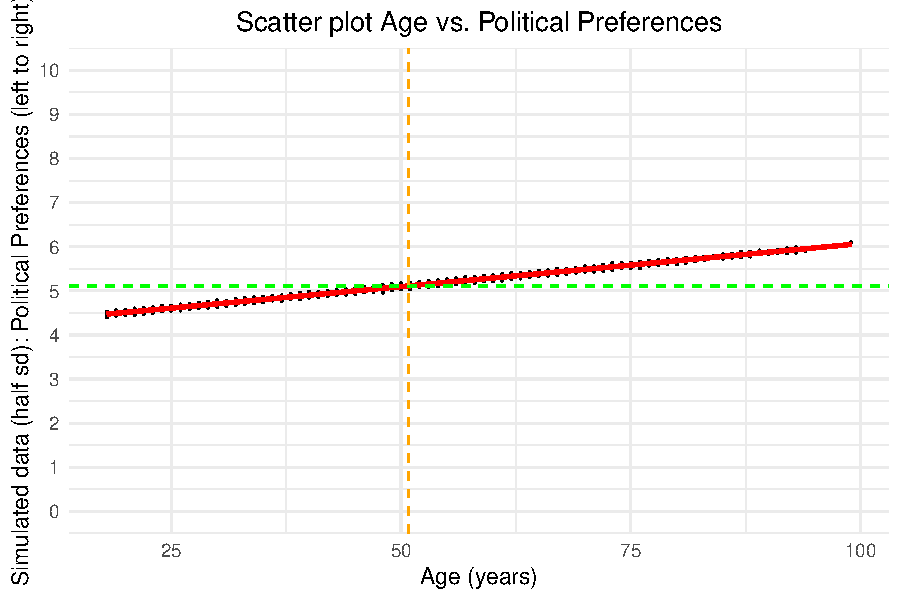
\includegraphics{_main_files/figure-latex/unnamed-chunk-85-1.pdf}

\hypertarget{simulated-data-1}{%
\subsection{Simulated data}\label{simulated-data-1}}

\begin{enumerate}
\def\labelenumi{\arabic{enumi}.}
\tightlist
\item
  In order to see the logic behind the \(R^2\), you will simulate what happens to it under different circumstances. To begin with, generate a random normal distribution of \(X\) and \(\epsilon\) both with mean 0 and standard deviation of 1.
\end{enumerate}

\begin{Shaded}
\begin{Highlighting}[]
\FunctionTok{set.seed}\NormalTok{(}\DecValTok{123}\NormalTok{)  }\CommentTok{\# For reproducibility}
\NormalTok{df }\OtherTok{\textless{}{-}} \FunctionTok{data.frame}\NormalTok{(}\AttributeTok{X =} \FunctionTok{rnorm}\NormalTok{(}\DecValTok{1000}\NormalTok{, }\AttributeTok{mean =} \DecValTok{0}\NormalTok{, }\AttributeTok{sd =} \DecValTok{1}\NormalTok{), }\AttributeTok{epsilon =} \FunctionTok{rnorm}\NormalTok{(}\DecValTok{100}\NormalTok{, }\AttributeTok{mean =} \DecValTok{0}\NormalTok{, }\AttributeTok{sd =} \DecValTok{1}\NormalTok{))}
\end{Highlighting}
\end{Shaded}

\begin{enumerate}
\def\labelenumi{\arabic{enumi}.}
\setcounter{enumi}{1}
\tightlist
\item
  Generate values for \(Y\) using the following data generating process. Graph it and regress \(Y\) on \(X\).
\end{enumerate}

\[Y=1+2X+\epsilon\]

\begin{Shaded}
\begin{Highlighting}[]
\NormalTok{df}\SpecialCharTok{$}\NormalTok{Y }\OtherTok{\textless{}{-}} \DecValTok{1}\SpecialCharTok{+}\DecValTok{2}\SpecialCharTok{*}\NormalTok{df}\SpecialCharTok{$}\NormalTok{X}\SpecialCharTok{+}\NormalTok{df}\SpecialCharTok{$}\NormalTok{epsilon}

\FunctionTok{ggplot}\NormalTok{(df, }\FunctionTok{aes}\NormalTok{(}\AttributeTok{x =}\NormalTok{ X, }\AttributeTok{y =}\NormalTok{ Y)) }\SpecialCharTok{+}
  \FunctionTok{geom\_smooth}\NormalTok{(}\AttributeTok{data =}\NormalTok{ df, }\FunctionTok{aes}\NormalTok{(}\AttributeTok{x =}\NormalTok{ X, }\AttributeTok{y =}\NormalTok{ Y), }
              \AttributeTok{method =} \StringTok{"lm"}\NormalTok{, }\AttributeTok{formula =}\NormalTok{ y }\SpecialCharTok{\textasciitilde{}}\NormalTok{ x, }\AttributeTok{color =} \StringTok{"red"}\NormalTok{, }\AttributeTok{se =} \ConstantTok{FALSE}\NormalTok{) }\SpecialCharTok{+}
  \FunctionTok{geom\_point}\NormalTok{()}
\end{Highlighting}
\end{Shaded}

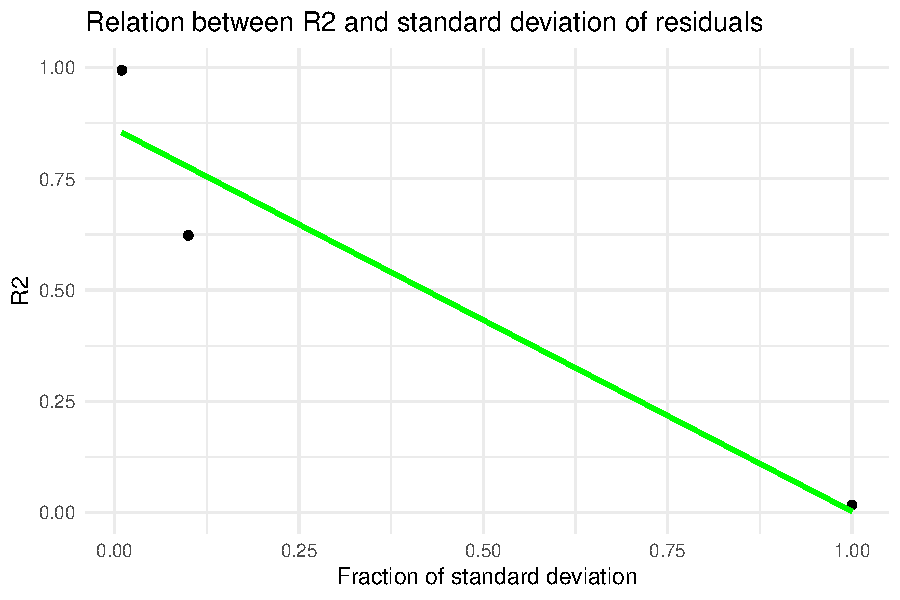
\includegraphics{_main_files/figure-latex/unnamed-chunk-87-1.pdf}

\begin{Shaded}
\begin{Highlighting}[]
\NormalTok{result1 }\OtherTok{\textless{}{-}} \FunctionTok{lm}\NormalTok{( Y }\SpecialCharTok{\textasciitilde{}}\NormalTok{ X, }\AttributeTok{data =}\NormalTok{ df)}
\FunctionTok{coef}\NormalTok{(result1)}
\end{Highlighting}
\end{Shaded}

\begin{verbatim}
## (Intercept)           X 
##    1.119243    2.043244
\end{verbatim}

\begin{enumerate}
\def\labelenumi{\arabic{enumi}.}
\setcounter{enumi}{1}
\tightlist
\item
  Now generate the normally distributed residuals with mean zero and variance equal to 5, 4, 3, 2, 1/2, 1/3, 1/4, and 1/5. Use each residual to create a new \(Y\). Then, keeping the same \(X\) unchanged, regress all the resulting \(Y\)s on \(X\). Present all the resulting \(R^2\) in a new dataframe to then graph the relation between the variance of the residual and the \(R^2\). What lesson do you take out of this graph?
\end{enumerate}

\begin{Shaded}
\begin{Highlighting}[]
\FunctionTok{set.seed}\NormalTok{(}\DecValTok{123}\NormalTok{)  }\CommentTok{\# For reproducibility}
\NormalTok{df}\SpecialCharTok{$}\NormalTok{ep5 }\OtherTok{\textless{}{-}} \FunctionTok{rnorm}\NormalTok{(}\DecValTok{1000}\NormalTok{, }\AttributeTok{mean =} \DecValTok{0}\NormalTok{, }\AttributeTok{sd =} \DecValTok{5}\NormalTok{)}
\NormalTok{df}\SpecialCharTok{$}\NormalTok{ep4 }\OtherTok{\textless{}{-}} \FunctionTok{rnorm}\NormalTok{(}\DecValTok{1000}\NormalTok{, }\AttributeTok{mean =} \DecValTok{0}\NormalTok{, }\AttributeTok{sd =} \DecValTok{4}\NormalTok{)}
\NormalTok{df}\SpecialCharTok{$}\NormalTok{ep3 }\OtherTok{\textless{}{-}} \FunctionTok{rnorm}\NormalTok{(}\DecValTok{1000}\NormalTok{, }\AttributeTok{mean =} \DecValTok{0}\NormalTok{, }\AttributeTok{sd =} \DecValTok{3}\NormalTok{)}
\NormalTok{df}\SpecialCharTok{$}\NormalTok{ep2 }\OtherTok{\textless{}{-}} \FunctionTok{rnorm}\NormalTok{(}\DecValTok{1000}\NormalTok{, }\AttributeTok{mean =} \DecValTok{0}\NormalTok{, }\AttributeTok{sd =} \DecValTok{2}\NormalTok{)}
\NormalTok{df}\SpecialCharTok{$}\NormalTok{ep1\_2 }\OtherTok{\textless{}{-}} \FunctionTok{rnorm}\NormalTok{(}\DecValTok{1000}\NormalTok{, }\AttributeTok{mean =} \DecValTok{0}\NormalTok{, }\AttributeTok{sd =} \DecValTok{1}\SpecialCharTok{/}\DecValTok{2}\NormalTok{)}
\NormalTok{df}\SpecialCharTok{$}\NormalTok{ep1\_3 }\OtherTok{\textless{}{-}} \FunctionTok{rnorm}\NormalTok{(}\DecValTok{1000}\NormalTok{, }\AttributeTok{mean =} \DecValTok{0}\NormalTok{, }\AttributeTok{sd =} \DecValTok{1}\SpecialCharTok{/}\DecValTok{3}\NormalTok{)}
\NormalTok{df}\SpecialCharTok{$}\NormalTok{ep1\_4 }\OtherTok{\textless{}{-}} \FunctionTok{rnorm}\NormalTok{(}\DecValTok{1000}\NormalTok{, }\AttributeTok{mean =} \DecValTok{0}\NormalTok{, }\AttributeTok{sd =} \DecValTok{1}\SpecialCharTok{/}\DecValTok{4}\NormalTok{)}
\NormalTok{df}\SpecialCharTok{$}\NormalTok{ep1\_5 }\OtherTok{\textless{}{-}} \FunctionTok{rnorm}\NormalTok{(}\DecValTok{1000}\NormalTok{, }\AttributeTok{mean =} \DecValTok{0}\NormalTok{, }\AttributeTok{sd =} \DecValTok{1}\SpecialCharTok{/}\DecValTok{5}\NormalTok{)}

\NormalTok{df}\SpecialCharTok{$}\NormalTok{Y5 }\OtherTok{\textless{}{-}} \DecValTok{1}\SpecialCharTok{+}\DecValTok{2}\SpecialCharTok{*}\NormalTok{df}\SpecialCharTok{$}\NormalTok{X}\SpecialCharTok{+}\NormalTok{df}\SpecialCharTok{$}\NormalTok{ep5}
\NormalTok{df}\SpecialCharTok{$}\NormalTok{Y4 }\OtherTok{\textless{}{-}} \DecValTok{1}\SpecialCharTok{+}\DecValTok{2}\SpecialCharTok{*}\NormalTok{df}\SpecialCharTok{$}\NormalTok{X}\SpecialCharTok{+}\NormalTok{df}\SpecialCharTok{$}\NormalTok{ep4}
\NormalTok{df}\SpecialCharTok{$}\NormalTok{Y3 }\OtherTok{\textless{}{-}} \DecValTok{1}\SpecialCharTok{+}\DecValTok{2}\SpecialCharTok{*}\NormalTok{df}\SpecialCharTok{$}\NormalTok{X}\SpecialCharTok{+}\NormalTok{df}\SpecialCharTok{$}\NormalTok{ep3}
\NormalTok{df}\SpecialCharTok{$}\NormalTok{Y2 }\OtherTok{\textless{}{-}} \DecValTok{1}\SpecialCharTok{+}\DecValTok{2}\SpecialCharTok{*}\NormalTok{df}\SpecialCharTok{$}\NormalTok{X}\SpecialCharTok{+}\NormalTok{df}\SpecialCharTok{$}\NormalTok{ep2}
\NormalTok{df}\SpecialCharTok{$}\NormalTok{Y\_2 }\OtherTok{\textless{}{-}} \DecValTok{1}\SpecialCharTok{+}\DecValTok{2}\SpecialCharTok{*}\NormalTok{df}\SpecialCharTok{$}\NormalTok{X}\SpecialCharTok{+}\NormalTok{df}\SpecialCharTok{$}\NormalTok{ep1\_2}
\NormalTok{df}\SpecialCharTok{$}\NormalTok{Y\_3 }\OtherTok{\textless{}{-}} \DecValTok{1}\SpecialCharTok{+}\DecValTok{2}\SpecialCharTok{*}\NormalTok{df}\SpecialCharTok{$}\NormalTok{X}\SpecialCharTok{+}\NormalTok{df}\SpecialCharTok{$}\NormalTok{ep1\_3}
\NormalTok{df}\SpecialCharTok{$}\NormalTok{Y\_4 }\OtherTok{\textless{}{-}} \DecValTok{1}\SpecialCharTok{+}\DecValTok{2}\SpecialCharTok{*}\NormalTok{df}\SpecialCharTok{$}\NormalTok{X}\SpecialCharTok{+}\NormalTok{df}\SpecialCharTok{$}\NormalTok{ep1\_4}
\NormalTok{df}\SpecialCharTok{$}\NormalTok{Y\_5 }\OtherTok{\textless{}{-}} \DecValTok{1}\SpecialCharTok{+}\DecValTok{2}\SpecialCharTok{*}\NormalTok{df}\SpecialCharTok{$}\NormalTok{X}\SpecialCharTok{+}\NormalTok{df}\SpecialCharTok{$}\NormalTok{ep1\_5}

\NormalTok{result5 }\OtherTok{\textless{}{-}} \FunctionTok{lm}\NormalTok{( Y5 }\SpecialCharTok{\textasciitilde{}}\NormalTok{ X, }\AttributeTok{data =}\NormalTok{ df)}
\NormalTok{result4 }\OtherTok{\textless{}{-}} \FunctionTok{lm}\NormalTok{( Y4 }\SpecialCharTok{\textasciitilde{}}\NormalTok{ X, }\AttributeTok{data =}\NormalTok{ df)}
\NormalTok{result3 }\OtherTok{\textless{}{-}} \FunctionTok{lm}\NormalTok{( Y3 }\SpecialCharTok{\textasciitilde{}}\NormalTok{ X, }\AttributeTok{data =}\NormalTok{ df)}
\NormalTok{result2 }\OtherTok{\textless{}{-}} \FunctionTok{lm}\NormalTok{( Y2 }\SpecialCharTok{\textasciitilde{}}\NormalTok{ X, }\AttributeTok{data =}\NormalTok{ df)}
\NormalTok{result\_2 }\OtherTok{\textless{}{-}} \FunctionTok{lm}\NormalTok{( Y\_2 }\SpecialCharTok{\textasciitilde{}}\NormalTok{ X, }\AttributeTok{data =}\NormalTok{ df)}
\NormalTok{result\_3 }\OtherTok{\textless{}{-}} \FunctionTok{lm}\NormalTok{( Y\_3 }\SpecialCharTok{\textasciitilde{}}\NormalTok{ X, }\AttributeTok{data =}\NormalTok{ df)}
\NormalTok{result\_4 }\OtherTok{\textless{}{-}} \FunctionTok{lm}\NormalTok{( Y\_4 }\SpecialCharTok{\textasciitilde{}}\NormalTok{ X, }\AttributeTok{data =}\NormalTok{ df)}
\NormalTok{result\_5 }\OtherTok{\textless{}{-}} \FunctionTok{lm}\NormalTok{( Y\_5 }\SpecialCharTok{\textasciitilde{}}\NormalTok{ X, }\AttributeTok{data =}\NormalTok{ df)}

\NormalTok{df\_rsqrd }\OtherTok{\textless{}{-}} \FunctionTok{data.frame}\NormalTok{(}
  \AttributeTok{SD =} \FunctionTok{c}\NormalTok{(}\DecValTok{5}\NormalTok{, }\DecValTok{4}\NormalTok{, }\DecValTok{3}\NormalTok{, }\DecValTok{2}\NormalTok{, }\DecValTok{1}\NormalTok{, }\DecValTok{1}\SpecialCharTok{/}\DecValTok{2}\NormalTok{, }\DecValTok{1}\SpecialCharTok{/}\DecValTok{3}\NormalTok{, }\DecValTok{1}\SpecialCharTok{/}\DecValTok{4}\NormalTok{, }\DecValTok{1}\SpecialCharTok{/}\DecValTok{5}\NormalTok{),}
  \AttributeTok{R2 =} \FunctionTok{c}\NormalTok{(}\FunctionTok{summary}\NormalTok{(result5)}\SpecialCharTok{$}\NormalTok{r.squared,}
         \FunctionTok{summary}\NormalTok{(result4)}\SpecialCharTok{$}\NormalTok{r.squared,}
         \FunctionTok{summary}\NormalTok{(result3)}\SpecialCharTok{$}\NormalTok{r.squared,}
         \FunctionTok{summary}\NormalTok{(result2)}\SpecialCharTok{$}\NormalTok{r.squared,}
         \FunctionTok{summary}\NormalTok{(result1)}\SpecialCharTok{$}\NormalTok{r.squared,}
         \FunctionTok{summary}\NormalTok{(result\_2)}\SpecialCharTok{$}\NormalTok{r.squared,}
         \FunctionTok{summary}\NormalTok{(result\_3)}\SpecialCharTok{$}\NormalTok{r.squared,}
         \FunctionTok{summary}\NormalTok{(result\_4)}\SpecialCharTok{$}\NormalTok{r.squared,}
         \FunctionTok{summary}\NormalTok{(result\_5)}\SpecialCharTok{$}\NormalTok{r.squared)}
\NormalTok{        )}

\FunctionTok{ggplot}\NormalTok{(df\_rsqrd, }\FunctionTok{aes}\NormalTok{(}\AttributeTok{x =}\NormalTok{ SD, }\AttributeTok{y =}\NormalTok{ R2)) }\SpecialCharTok{+}
  \FunctionTok{geom\_smooth}\NormalTok{(}\AttributeTok{data =}\NormalTok{ df\_rsqrd, }\FunctionTok{aes}\NormalTok{(}\AttributeTok{x =}\NormalTok{ SD, }\AttributeTok{y =}\NormalTok{ R2), }
              \AttributeTok{method =} \StringTok{"lm"}\NormalTok{, }\AttributeTok{formula =}\NormalTok{ y }\SpecialCharTok{\textasciitilde{}}\NormalTok{ x, }\AttributeTok{color =} \StringTok{"red"}\NormalTok{, }\AttributeTok{se =} \ConstantTok{FALSE}\NormalTok{) }\SpecialCharTok{+}
  \FunctionTok{geom\_point}\NormalTok{()}
\end{Highlighting}
\end{Shaded}

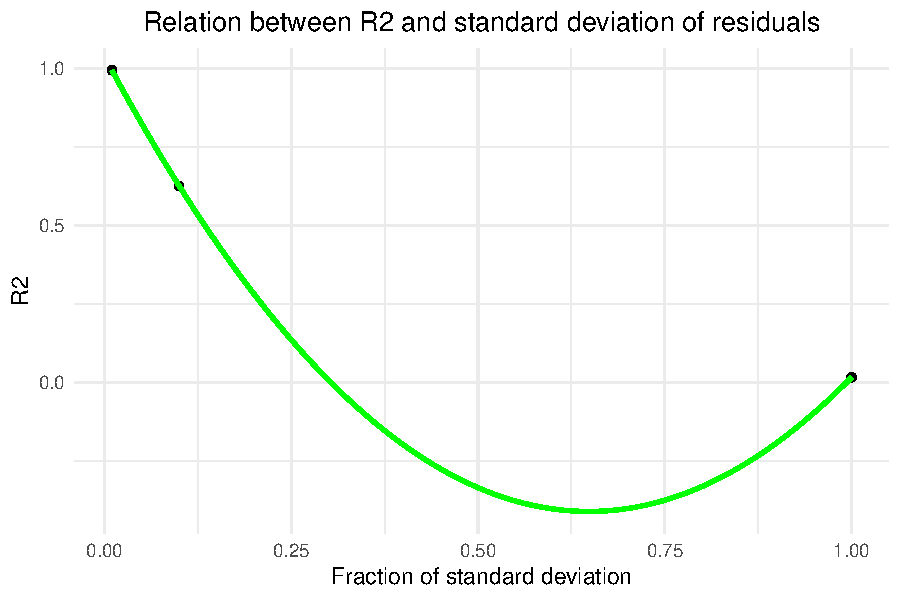
\includegraphics{_main_files/figure-latex/unnamed-chunk-89-1.pdf}

As shown in \href{https://en.wikipedia.org/wiki/Coefficient_of_determination}{this} entry, the bigger the sum of squared residuals is as a share of the regressand's variance, the less capable out model to capture the relation between our regressand and regressor. Thus, as the graph shows, the smaller variance of the residual, the higher the \(R^2\). In other words, the more dispersed observations are around \emph{each section of the regression line}, the lower the goodness of fit our model has to describe our data.

\begin{enumerate}
\def\labelenumi{\arabic{enumi}.}
\setcounter{enumi}{2}
\tightlist
\item
  In order to see the logic behind the \(R^2\), first estimate the linear regression of \texttt{LeftToRight} on \texttt{Age}. Generate the variable \texttt{predicted\_LeftToRight} with the generated parameters using \href{https://www.statology.org/r-lm-predict/}{\texttt{predict()}} from the point 3 of the previous section (i.e., the one using real data).Generate the graph \texttt{predicted\_LeftToRight} vs \texttt{Age}.
\end{enumerate}

Report the regression here.

\begin{Shaded}
\begin{Highlighting}[]
\NormalTok{result }\OtherTok{\textless{}{-}} \FunctionTok{lm}\NormalTok{(LeftToRight }\SpecialCharTok{\textasciitilde{}}\NormalTok{ age, }\AttributeTok{data =}\NormalTok{ selects19)}
\NormalTok{selects19}\SpecialCharTok{$}\NormalTok{predicted\_LeftToRight }\OtherTok{\textless{}{-}} \FunctionTok{predict}\NormalTok{(result)}

\NormalTok{coeffs1 }\OtherTok{\textless{}{-}} \FunctionTok{coef}\NormalTok{(result)}
\NormalTok{rsq\_sd1 }\OtherTok{\textless{}{-}} \FunctionTok{summary}\NormalTok{(result)}\SpecialCharTok{$}\NormalTok{r.squared}
\FunctionTok{cat}\NormalTok{(}\StringTok{\textquotesingle{}The R2 is: \textquotesingle{}}\NormalTok{, rsq\_sd1, }\StringTok{\textquotesingle{}}\SpecialCharTok{\textbackslash{}n\textbackslash{}n}\StringTok{Intercept:\textquotesingle{}}\NormalTok{,}\FunctionTok{unname}\NormalTok{(coeffs1[}\DecValTok{1}\NormalTok{]), }\StringTok{\textquotesingle{}}\SpecialCharTok{\textbackslash{}n\textbackslash{}n}\StringTok{Slope:\textquotesingle{}}\NormalTok{, }\FunctionTok{unname}\NormalTok{(coeffs1[}\DecValTok{2}\NormalTok{]))}
\end{Highlighting}
\end{Shaded}

\begin{verbatim}
## The R2 is:  0.0161515 
## 
## Intercept: 4.122055 
## 
## Slope: 0.01948902
\end{verbatim}

Report the graph here.

\begin{Shaded}
\begin{Highlighting}[]
\CommentTok{\# Calculate means for Y and X}
\NormalTok{mean\_LeftRight }\OtherTok{\textless{}{-}} \FunctionTok{mean}\NormalTok{(selects19}\SpecialCharTok{$}\NormalTok{LeftToRight, }\AttributeTok{na.rm =} \ConstantTok{TRUE}\NormalTok{)}
\NormalTok{mean\_age }\OtherTok{\textless{}{-}} \FunctionTok{mean}\NormalTok{(selects19}\SpecialCharTok{$}\NormalTok{age, }\AttributeTok{na.rm =} \ConstantTok{TRUE}\NormalTok{)}

\CommentTok{\# Create a scatter plot}
\FunctionTok{ggplot}\NormalTok{(selects19, }\FunctionTok{aes}\NormalTok{(}\AttributeTok{x =}\NormalTok{ age, }\AttributeTok{y =}\NormalTok{ predicted\_LeftToRight)) }\SpecialCharTok{+}
  \FunctionTok{geom\_smooth}\NormalTok{(}\AttributeTok{method =} \StringTok{"lm"}\NormalTok{, }\AttributeTok{formula =}\NormalTok{ y }\SpecialCharTok{\textasciitilde{}}\NormalTok{ x, }\AttributeTok{se =} \ConstantTok{FALSE}\NormalTok{, }\AttributeTok{color =} \StringTok{"red"}\NormalTok{) }\SpecialCharTok{+}  \CommentTok{\# Adding the regression line}
  \FunctionTok{geom\_hline}\NormalTok{(}\AttributeTok{yintercept =}\NormalTok{ mean\_LeftRight, }\AttributeTok{linetype =} \StringTok{"dashed"}\NormalTok{, }\AttributeTok{color =} \StringTok{"green"}\NormalTok{) }\SpecialCharTok{+}  \CommentTok{\# Horizontal line at the mean of y}
  \FunctionTok{geom\_vline}\NormalTok{(}\AttributeTok{xintercept =}\NormalTok{ mean\_age, }\AttributeTok{linetype =} \StringTok{"dashed"}\NormalTok{, }\AttributeTok{color =} \StringTok{"orange"}\NormalTok{) }\SpecialCharTok{+}  \CommentTok{\# Vertical line at the mean of x}
  \FunctionTok{scale\_y\_continuous}\NormalTok{(}
    \AttributeTok{limits =} \FunctionTok{c}\NormalTok{(}\DecValTok{0}\NormalTok{, }\DecValTok{10}\NormalTok{),}
    \AttributeTok{breaks =} \FunctionTok{seq}\NormalTok{(}\DecValTok{0}\NormalTok{, }\DecValTok{10}\NormalTok{, }\AttributeTok{by =} \DecValTok{1}\NormalTok{)}
\NormalTok{  ) }\SpecialCharTok{+}
  \FunctionTok{theme\_minimal}\NormalTok{() }\SpecialCharTok{+}
  \FunctionTok{theme}\NormalTok{(}
    \AttributeTok{plot.title =} \FunctionTok{element\_text}\NormalTok{(}\AttributeTok{hjust =} \FloatTok{0.5}\NormalTok{), }\CommentTok{\# Center the plot title}
    \AttributeTok{panel.grid.major.y =} \FunctionTok{element\_line}\NormalTok{(}\AttributeTok{color =} \StringTok{"grey80"}\NormalTok{, }\AttributeTok{size =} \FloatTok{0.5}\NormalTok{), }\CommentTok{\# Style for major Y grid lines}
    \AttributeTok{panel.grid.minor.y =} \FunctionTok{element\_blank}\NormalTok{() }\CommentTok{\# Remove minor Y grid lines}
\NormalTok{  ) }\SpecialCharTok{+}
  \FunctionTok{labs}\NormalTok{(}
    \AttributeTok{x =} \StringTok{"Age (years)"}\NormalTok{,}
    \AttributeTok{y =} \StringTok{"Political Preferences (left to right)"}\NormalTok{,}
    \AttributeTok{title =} \StringTok{"Scatter plot Age vs. Political Preferences (determ. sim.)"}
\NormalTok{  )}
\end{Highlighting}
\end{Shaded}

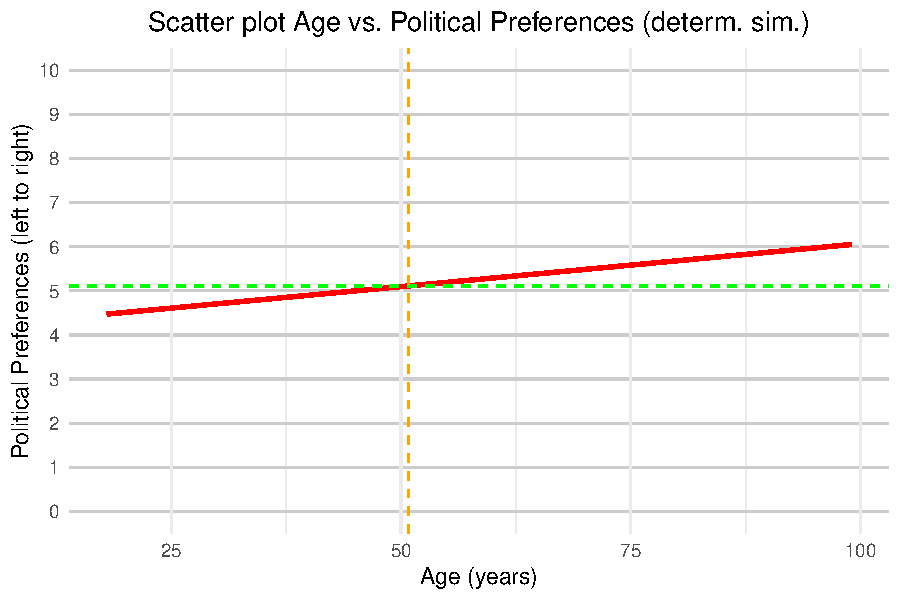
\includegraphics{_main_files/figure-latex/unnamed-chunk-91-1.pdf}

\begin{enumerate}
\def\labelenumi{\arabic{enumi}.}
\setcounter{enumi}{3}
\tightlist
\item
  Now generate the normally distributed residuals with mean zero and the same variance as the residuals of the model from the previous point.
\end{enumerate}

\begin{Shaded}
\begin{Highlighting}[]
\CommentTok{\# Calculate the variance of the residuals}
\NormalTok{selects19}\SpecialCharTok{$}\NormalTok{residual }\OtherTok{\textless{}{-}} \FunctionTok{resid}\NormalTok{(result)}
\NormalTok{residual\_sd }\OtherTok{\textless{}{-}} \FunctionTok{sqrt}\NormalTok{(}\FunctionTok{var}\NormalTok{(}\FunctionTok{resid}\NormalTok{(result)))}

\CommentTok{\# Set the seed for reproducibility}
\FunctionTok{set.seed}\NormalTok{(}\DecValTok{0}\NormalTok{)}
\NormalTok{selects19}\SpecialCharTok{$}\NormalTok{NormResiduals1 }\OtherTok{\textless{}{-}} \FunctionTok{rnorm}\NormalTok{(}\FunctionTok{nrow}\NormalTok{(selects19), }\AttributeTok{mean =} \DecValTok{0}\NormalTok{, }\AttributeTok{sd =}\NormalTok{ residual\_sd)}
\end{Highlighting}
\end{Shaded}

\begin{enumerate}
\def\labelenumi{\arabic{enumi}.}
\setcounter{enumi}{4}
\tightlist
\item
  Simulate new data using both the deterministic (i.e., the the parameters estimated immediately above) and stochastic component (i.e., the residuals form the previous point). Graph the simulated data.
\end{enumerate}

\begin{Shaded}
\begin{Highlighting}[]
\NormalTok{selects19}\SpecialCharTok{$}\NormalTok{Sim\_LeftToRight\_Det\_Stoch }\OtherTok{\textless{}{-}}\NormalTok{ selects19}\SpecialCharTok{$}\NormalTok{predicted\_LeftToRight }\SpecialCharTok{+}\NormalTok{ selects19}\SpecialCharTok{$}\NormalTok{NormResiduals1}

\CommentTok{\#Means for Y and X}
\NormalTok{mean\_LeftRight }\OtherTok{\textless{}{-}} \FunctionTok{mean}\NormalTok{(selects19}\SpecialCharTok{$}\NormalTok{Sim\_LeftToRight\_Det\_Stoch, }\AttributeTok{na.rm =} \ConstantTok{TRUE}\NormalTok{)}
\NormalTok{mean\_age }\OtherTok{\textless{}{-}} \FunctionTok{mean}\NormalTok{(selects19}\SpecialCharTok{$}\NormalTok{age, }\AttributeTok{na.rm =} \ConstantTok{TRUE}\NormalTok{)}

\CommentTok{\# Create a scatter plot}
\FunctionTok{ggplot}\NormalTok{(selects19, }\FunctionTok{aes}\NormalTok{(}\AttributeTok{x =}\NormalTok{ age, }\AttributeTok{y =}\NormalTok{ Sim\_LeftToRight\_Det\_Stoch)) }\SpecialCharTok{+}
  \FunctionTok{geom\_point}\NormalTok{(}\AttributeTok{size =} \DecValTok{0}\NormalTok{) }\SpecialCharTok{+}
  \FunctionTok{geom\_smooth}\NormalTok{(}\AttributeTok{method =} \StringTok{"lm"}\NormalTok{, }\AttributeTok{formula =}\NormalTok{ y }\SpecialCharTok{\textasciitilde{}}\NormalTok{ x, }\AttributeTok{se =} \ConstantTok{FALSE}\NormalTok{, }\AttributeTok{color =} \StringTok{"red"}\NormalTok{) }\SpecialCharTok{+}  \CommentTok{\# Adding the regression line}
  \FunctionTok{geom\_hline}\NormalTok{(}\AttributeTok{yintercept =}\NormalTok{ mean\_LeftRight, }\AttributeTok{linetype =} \StringTok{"dashed"}\NormalTok{, }\AttributeTok{color =} \StringTok{"green"}\NormalTok{) }\SpecialCharTok{+}  \CommentTok{\# Horizontal line at the mean of y}
  \FunctionTok{geom\_vline}\NormalTok{(}\AttributeTok{xintercept =}\NormalTok{ mean\_age, }\AttributeTok{linetype =} \StringTok{"dashed"}\NormalTok{, }\AttributeTok{color =} \StringTok{"orange"}\NormalTok{) }\SpecialCharTok{+}  \CommentTok{\# Vertical line at the mean of x}
  \FunctionTok{theme\_minimal}\NormalTok{() }\SpecialCharTok{+}
  \FunctionTok{theme}\NormalTok{(}\AttributeTok{plot.title =} \FunctionTok{element\_text}\NormalTok{(}\AttributeTok{hjust =} \FloatTok{0.5}\NormalTok{)) }\SpecialCharTok{+}
  \FunctionTok{scale\_y\_continuous}\NormalTok{(}
    \AttributeTok{limits =} \FunctionTok{c}\NormalTok{(}\DecValTok{0}\NormalTok{, }\DecValTok{10}\NormalTok{),}
    \AttributeTok{breaks =} \FunctionTok{seq}\NormalTok{(}\DecValTok{0}\NormalTok{, }\DecValTok{10}\NormalTok{, }\AttributeTok{by =} \DecValTok{1}\NormalTok{)) }\SpecialCharTok{+}
  \FunctionTok{theme\_minimal}\NormalTok{() }\SpecialCharTok{+}
  \FunctionTok{theme}\NormalTok{(}
    \AttributeTok{plot.title =} \FunctionTok{element\_text}\NormalTok{(}\AttributeTok{hjust =} \FloatTok{0.5}\NormalTok{), }\CommentTok{\# Center the plot title}
    \AttributeTok{panel.grid.major.y =} \FunctionTok{element\_line}\NormalTok{(}\AttributeTok{color =} \StringTok{"grey80"}\NormalTok{, }\AttributeTok{size =} \FloatTok{0.5}\NormalTok{), }\CommentTok{\# Style for major Y grid lines}
    \AttributeTok{panel.grid.minor.y =} \FunctionTok{element\_blank}\NormalTok{() }\CommentTok{\# Remove minor Y grid lines}
\NormalTok{  ) }\SpecialCharTok{+}
  \FunctionTok{labs}\NormalTok{(}
    \AttributeTok{x =} \StringTok{"Age (years)"}\NormalTok{,}
    \AttributeTok{y =} \StringTok{"Simulation: Political Preferences (left to right)"}\NormalTok{,}
    \AttributeTok{title =} \StringTok{"Scatter plot Age vs. Political Preferences }\SpecialCharTok{\textbackslash{}n}\StringTok{(determ.\& stoch. sim.)"}
\NormalTok{  )}
\end{Highlighting}
\end{Shaded}

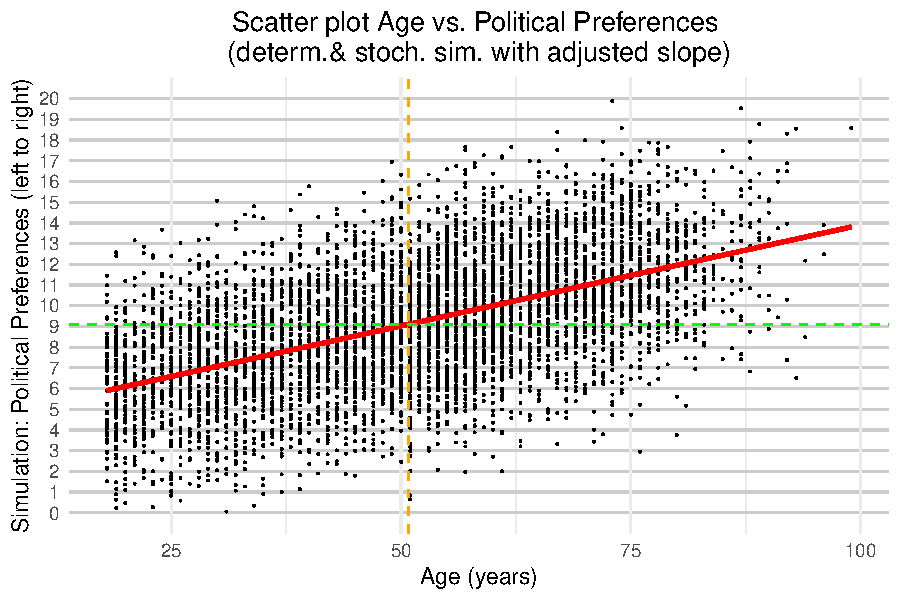
\includegraphics{_main_files/figure-latex/unnamed-chunk-93-1.pdf}

\begin{enumerate}
\def\labelenumi{\arabic{enumi}.}
\setcounter{enumi}{4}
\tightlist
\item
  Now, estimate the regression between the real \texttt{age} and simulated \texttt{Sim\_LeftToRight\_Det\_Stoch}. Once you do that, generate the \(R^2\) for the model.
\end{enumerate}

\begin{Shaded}
\begin{Highlighting}[]
\NormalTok{result }\OtherTok{\textless{}{-}} \FunctionTok{lm}\NormalTok{(LeftToRight }\SpecialCharTok{\textasciitilde{}}\NormalTok{ age, }\AttributeTok{data =}\NormalTok{ selects19)}
\NormalTok{rsq\_sd1 }\OtherTok{\textless{}{-}} \FunctionTok{summary}\NormalTok{(result)}\SpecialCharTok{$}\NormalTok{r.squared}
\FunctionTok{cat}\NormalTok{(}\StringTok{\textquotesingle{}The R2 is: \textquotesingle{}}\NormalTok{, rsq\_sd1)}
\end{Highlighting}
\end{Shaded}

\begin{verbatim}
## The R2 is:  0.0161515
\end{verbatim}

\begin{enumerate}
\def\labelenumi{\arabic{enumi}.}
\setcounter{enumi}{6}
\tightlist
\item
  Repeat the previous three points but use half the standard deviation of the model of point 1. Is the \(R^2\) lower now? Why? See \href{https://en.wikipedia.org/wiki/Coefficient_of_determination}{this} entry to understand the intuition: pay special attention to the graph with the red and blue squares.
\end{enumerate}

Generate the residuals here.

\begin{Shaded}
\begin{Highlighting}[]
\CommentTok{\# Set the seed for reproducibility}
\FunctionTok{set.seed}\NormalTok{(}\DecValTok{0}\NormalTok{)}
\NormalTok{selects19}\SpecialCharTok{$}\NormalTok{NormResiduals10 }\OtherTok{\textless{}{-}} \FunctionTok{rnorm}\NormalTok{(}\FunctionTok{nrow}\NormalTok{(selects19), }\AttributeTok{mean =} \DecValTok{0}\NormalTok{, }\AttributeTok{sd =}\NormalTok{ residual\_sd}\SpecialCharTok{*}\FloatTok{0.1}\NormalTok{)}
\end{Highlighting}
\end{Shaded}

Simulate new data and graph it here.

\begin{Shaded}
\begin{Highlighting}[]
\NormalTok{selects19}\SpecialCharTok{$}\NormalTok{Sim\_LeftToRight\_Det\_Stoch\_sd10 }\OtherTok{\textless{}{-}}\NormalTok{ selects19}\SpecialCharTok{$}\NormalTok{predicted\_LeftToRight }\SpecialCharTok{+}\NormalTok{ selects19}\SpecialCharTok{$}\NormalTok{NormResiduals10}

\CommentTok{\#Means for Y and X}
\NormalTok{mean\_LeftRight }\OtherTok{\textless{}{-}} \FunctionTok{mean}\NormalTok{(selects19}\SpecialCharTok{$}\NormalTok{Sim\_LeftToRight\_Det\_Stoch\_sd10, }\AttributeTok{na.rm =} \ConstantTok{TRUE}\NormalTok{)}
\NormalTok{mean\_age }\OtherTok{\textless{}{-}} \FunctionTok{mean}\NormalTok{(selects19}\SpecialCharTok{$}\NormalTok{age, }\AttributeTok{na.rm =} \ConstantTok{TRUE}\NormalTok{)}

\CommentTok{\# Create a scatter plot}
\FunctionTok{ggplot}\NormalTok{(selects19, }\FunctionTok{aes}\NormalTok{(}\AttributeTok{x =}\NormalTok{ age, }\AttributeTok{y =}\NormalTok{ Sim\_LeftToRight\_Det\_Stoch\_sd10)) }\SpecialCharTok{+}
  \FunctionTok{geom\_point}\NormalTok{(}\AttributeTok{size =} \DecValTok{0}\NormalTok{) }\SpecialCharTok{+}
  \FunctionTok{geom\_smooth}\NormalTok{(}\AttributeTok{method =} \StringTok{"lm"}\NormalTok{, }\AttributeTok{formula =}\NormalTok{ y }\SpecialCharTok{\textasciitilde{}}\NormalTok{ x, }\AttributeTok{se =} \ConstantTok{FALSE}\NormalTok{, }\AttributeTok{color =} \StringTok{"red"}\NormalTok{) }\SpecialCharTok{+}  \CommentTok{\# Adding the regression line}
  \FunctionTok{geom\_hline}\NormalTok{(}\AttributeTok{yintercept =}\NormalTok{ mean\_LeftRight, }\AttributeTok{linetype =} \StringTok{"dashed"}\NormalTok{, }\AttributeTok{color =} \StringTok{"green"}\NormalTok{) }\SpecialCharTok{+}  \CommentTok{\# Horizontal line at the mean of y}
  \FunctionTok{geom\_vline}\NormalTok{(}\AttributeTok{xintercept =}\NormalTok{ mean\_age, }\AttributeTok{linetype =} \StringTok{"dashed"}\NormalTok{, }\AttributeTok{color =} \StringTok{"orange"}\NormalTok{) }\SpecialCharTok{+}  \CommentTok{\# Vertical line at the mean of x}
  \FunctionTok{scale\_y\_continuous}\NormalTok{(}
    \AttributeTok{limits =} \FunctionTok{c}\NormalTok{(}\DecValTok{0}\NormalTok{, }\DecValTok{10}\NormalTok{),}
    \AttributeTok{breaks =} \FunctionTok{seq}\NormalTok{(}\DecValTok{0}\NormalTok{, }\DecValTok{10}\NormalTok{, }\AttributeTok{by =} \DecValTok{1}\NormalTok{)) }\SpecialCharTok{+}
  \FunctionTok{theme\_minimal}\NormalTok{() }\SpecialCharTok{+}
  \FunctionTok{theme}\NormalTok{(}\AttributeTok{plot.title =} \FunctionTok{element\_text}\NormalTok{(}\AttributeTok{hjust =} \FloatTok{0.5}\NormalTok{)) }\SpecialCharTok{+}
  \FunctionTok{labs}\NormalTok{(}
    \AttributeTok{x =} \StringTok{"Age (years)"}\NormalTok{,}
    \AttributeTok{y =} \StringTok{"Simulated data (half sd): Political Preferences (left to right)"}\NormalTok{,}
    \AttributeTok{title =} \StringTok{"Scatter plot Age vs. Political Preferences"}
\NormalTok{  )}
\end{Highlighting}
\end{Shaded}

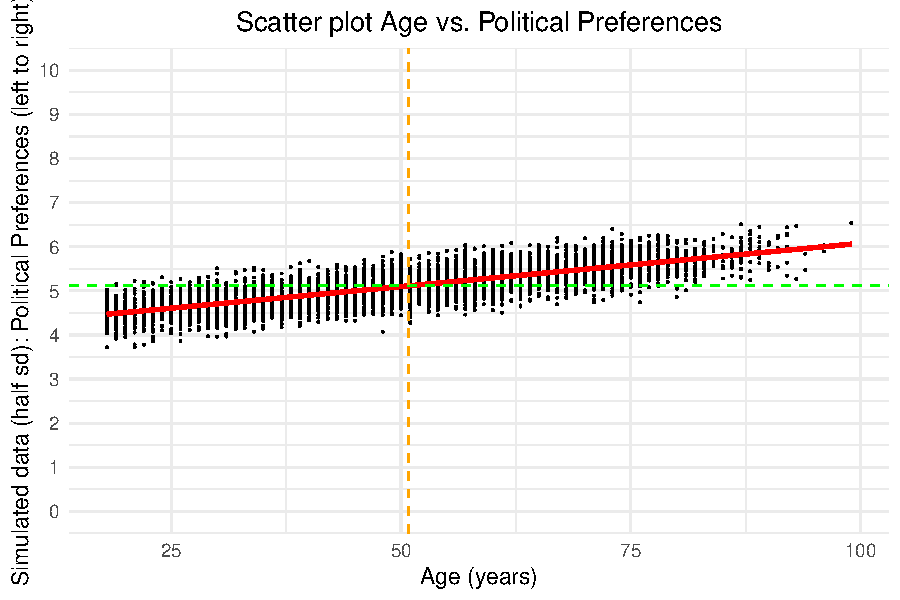
\includegraphics{_main_files/figure-latex/unnamed-chunk-96-1.pdf}

Report the new \(R^2\) here:

\begin{Shaded}
\begin{Highlighting}[]
\NormalTok{result }\OtherTok{\textless{}{-}} \FunctionTok{lm}\NormalTok{(Sim\_LeftToRight\_Det\_Stoch\_sd10 }\SpecialCharTok{\textasciitilde{}}\NormalTok{ age, }\AttributeTok{data =}\NormalTok{ selects19)}
\NormalTok{rsq\_sd10 }\OtherTok{\textless{}{-}} \FunctionTok{summary}\NormalTok{(result)}\SpecialCharTok{$}\NormalTok{r.squared}
\FunctionTok{cat}\NormalTok{(}\StringTok{\textquotesingle{}The R2 is: \textquotesingle{}}\NormalTok{, rsq\_sd10)}
\end{Highlighting}
\end{Shaded}

\begin{verbatim}
## The R2 is:  0.625503
\end{verbatim}

\begin{enumerate}
\def\labelenumi{\arabic{enumi}.}
\setcounter{enumi}{7}
\tightlist
\item
  Repeat the previous point but use a hundredth the standard deviation of the model of point 1. Is the \(R^2\) lower now? Why?
\end{enumerate}

Generate the residuals here.

\begin{Shaded}
\begin{Highlighting}[]
\CommentTok{\# Set the seed for reproducibility}
\FunctionTok{set.seed}\NormalTok{(}\DecValTok{0}\NormalTok{)}
\NormalTok{selects19}\SpecialCharTok{$}\NormalTok{NormResiduals100 }\OtherTok{\textless{}{-}} \FunctionTok{rnorm}\NormalTok{(}\FunctionTok{nrow}\NormalTok{(selects19), }\AttributeTok{mean =} \DecValTok{0}\NormalTok{, }\AttributeTok{sd =}\NormalTok{ residual\_sd}\SpecialCharTok{*}\FloatTok{0.01}\NormalTok{)}
\end{Highlighting}
\end{Shaded}

Simulate new data and graph it here.

\begin{Shaded}
\begin{Highlighting}[]
\NormalTok{selects19}\SpecialCharTok{$}\NormalTok{Sim\_LeftToRight\_Det\_Stoch\_hsd }\OtherTok{\textless{}{-}}\NormalTok{ selects19}\SpecialCharTok{$}\NormalTok{predicted\_LeftToRight }\SpecialCharTok{+}\NormalTok{ selects19}\SpecialCharTok{$}\NormalTok{NormResiduals100}

\CommentTok{\#Means for Y and X}
\NormalTok{mean\_LeftRight }\OtherTok{\textless{}{-}} \FunctionTok{mean}\NormalTok{(selects19}\SpecialCharTok{$}\NormalTok{Sim\_LeftToRight\_Det\_Stoch\_hsd, }\AttributeTok{na.rm =} \ConstantTok{TRUE}\NormalTok{)}
\NormalTok{mean\_age }\OtherTok{\textless{}{-}} \FunctionTok{mean}\NormalTok{(selects19}\SpecialCharTok{$}\NormalTok{age, }\AttributeTok{na.rm =} \ConstantTok{TRUE}\NormalTok{)}

\CommentTok{\# Create a scatter plot}
\FunctionTok{ggplot}\NormalTok{(selects19, }\FunctionTok{aes}\NormalTok{(}\AttributeTok{x =}\NormalTok{ age, }\AttributeTok{y =}\NormalTok{ Sim\_LeftToRight\_Det\_Stoch\_hsd)) }\SpecialCharTok{+}
  \FunctionTok{geom\_point}\NormalTok{(}\AttributeTok{size =} \DecValTok{0}\NormalTok{) }\SpecialCharTok{+}
  \FunctionTok{geom\_smooth}\NormalTok{(}\AttributeTok{method =} \StringTok{"lm"}\NormalTok{, }\AttributeTok{formula =}\NormalTok{ y }\SpecialCharTok{\textasciitilde{}}\NormalTok{ x, }\AttributeTok{se =} \ConstantTok{FALSE}\NormalTok{, }\AttributeTok{color =} \StringTok{"red"}\NormalTok{) }\SpecialCharTok{+}  \CommentTok{\# Adding the regression line}
  \FunctionTok{geom\_hline}\NormalTok{(}\AttributeTok{yintercept =}\NormalTok{ mean\_LeftRight, }\AttributeTok{linetype =} \StringTok{"dashed"}\NormalTok{, }\AttributeTok{color =} \StringTok{"green"}\NormalTok{) }\SpecialCharTok{+}  \CommentTok{\# Horizontal line at the mean of y}
  \FunctionTok{geom\_vline}\NormalTok{(}\AttributeTok{xintercept =}\NormalTok{ mean\_age, }\AttributeTok{linetype =} \StringTok{"dashed"}\NormalTok{, }\AttributeTok{color =} \StringTok{"orange"}\NormalTok{) }\SpecialCharTok{+}  \CommentTok{\# Vertical line at the mean of x}
  \FunctionTok{scale\_y\_continuous}\NormalTok{(}
    \AttributeTok{limits =} \FunctionTok{c}\NormalTok{(}\DecValTok{0}\NormalTok{, }\DecValTok{10}\NormalTok{),}
    \AttributeTok{breaks =} \FunctionTok{seq}\NormalTok{(}\DecValTok{0}\NormalTok{, }\DecValTok{10}\NormalTok{, }\AttributeTok{by =} \DecValTok{1}\NormalTok{)) }\SpecialCharTok{+}
  \FunctionTok{theme\_minimal}\NormalTok{() }\SpecialCharTok{+}
  \FunctionTok{theme}\NormalTok{(}\AttributeTok{plot.title =} \FunctionTok{element\_text}\NormalTok{(}\AttributeTok{hjust =} \FloatTok{0.5}\NormalTok{)) }\SpecialCharTok{+}
  \FunctionTok{labs}\NormalTok{(}
    \AttributeTok{x =} \StringTok{"Age (years)"}\NormalTok{,}
    \AttributeTok{y =} \StringTok{"Simulated data (half sd): Political Preferences (left to right)"}\NormalTok{,}
    \AttributeTok{title =} \StringTok{"Scatter plot Age vs. Political Preferences"}
\NormalTok{  )}
\end{Highlighting}
\end{Shaded}

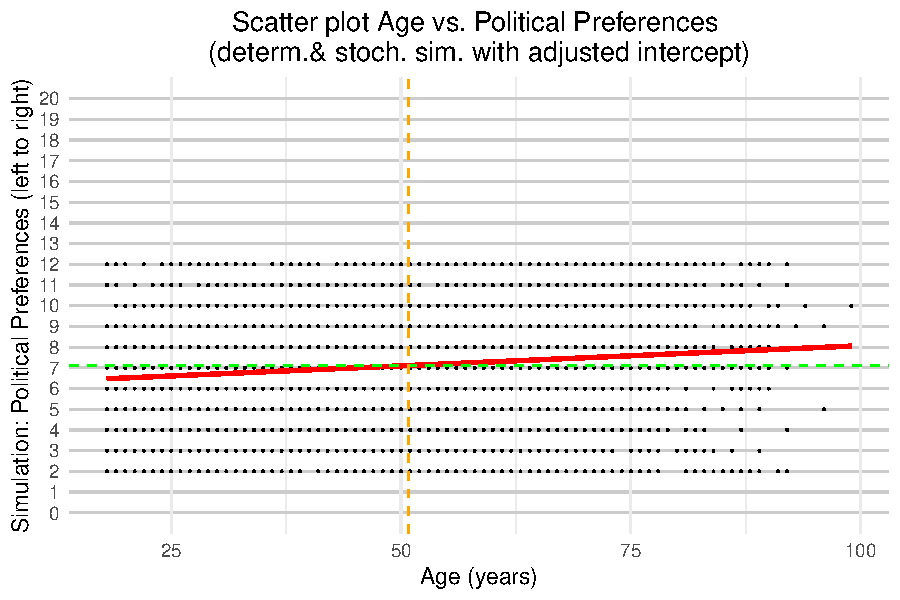
\includegraphics{_main_files/figure-latex/unnamed-chunk-99-1.pdf}

Report the new \(R^2\) here:

\begin{Shaded}
\begin{Highlighting}[]
\NormalTok{result }\OtherTok{\textless{}{-}} \FunctionTok{lm}\NormalTok{(Sim\_LeftToRight\_Det\_Stoch\_hsd }\SpecialCharTok{\textasciitilde{}}\NormalTok{ age, }\AttributeTok{data =}\NormalTok{ selects19)}
\NormalTok{rsq\_sd100 }\OtherTok{\textless{}{-}} \FunctionTok{summary}\NormalTok{(result)}\SpecialCharTok{$}\NormalTok{r.squared}
\FunctionTok{cat}\NormalTok{(}\StringTok{\textquotesingle{}The R2 is: \textquotesingle{}}\NormalTok{, rsq\_sd100)}
\end{Highlighting}
\end{Shaded}

\begin{verbatim}
## The R2 is:  0.9939772
\end{verbatim}

\begin{enumerate}
\def\labelenumi{\arabic{enumi}.}
\setcounter{enumi}{8}
\tightlist
\item
  Present in a table the \(R^2\) for each value of the standard deviation.
\end{enumerate}

\begin{Shaded}
\begin{Highlighting}[]
\NormalTok{table }\OtherTok{\textless{}{-}} \FunctionTok{data.frame}\NormalTok{(}
  \AttributeTok{SD =} \FunctionTok{c}\NormalTok{(}\DecValTok{1}\NormalTok{, }\FloatTok{0.1}\NormalTok{, }\FloatTok{0.01}\NormalTok{),}
  \AttributeTok{R2 =} \FunctionTok{c}\NormalTok{(rsq\_sd1, rsq\_sd10, rsq\_sd100)    }\CommentTok{\# Replace these with the actual R{-}squared values}
\NormalTok{)}

\FunctionTok{print}\NormalTok{(table)}
\end{Highlighting}
\end{Shaded}

\begin{verbatim}
##     SD        R2
## 1 1.00 0.0161515
## 2 0.10 0.6255030
## 3 0.01 0.9939772
\end{verbatim}

\begin{enumerate}
\def\labelenumi{\arabic{enumi}.}
\setcounter{enumi}{9}
\tightlist
\item
  Graph \(R^2\) agains the standard deviation fraction. Fit a linear regression line.
\end{enumerate}

\begin{Shaded}
\begin{Highlighting}[]
\FunctionTok{ggplot}\NormalTok{(table, }\FunctionTok{aes}\NormalTok{(}\AttributeTok{x =}\NormalTok{ SD, }\AttributeTok{y =}\NormalTok{ R2)) }\SpecialCharTok{+}
  \FunctionTok{geom\_point}\NormalTok{(}\AttributeTok{size =} \DecValTok{0}\NormalTok{) }\SpecialCharTok{+}
  \FunctionTok{geom\_smooth}\NormalTok{(}\AttributeTok{method =} \StringTok{"lm"}\NormalTok{, }\AttributeTok{formula =}\NormalTok{ y }\SpecialCharTok{\textasciitilde{}}\NormalTok{ x, }\AttributeTok{se =} \ConstantTok{FALSE}\NormalTok{, }\AttributeTok{color =} \StringTok{"green"}\NormalTok{)}\SpecialCharTok{+}
  \FunctionTok{theme\_minimal}\NormalTok{() }\SpecialCharTok{+}
  \FunctionTok{theme}\NormalTok{(}\AttributeTok{plot.title =} \FunctionTok{element\_text}\NormalTok{(}\AttributeTok{hjust =} \FloatTok{0.5}\NormalTok{)) }\SpecialCharTok{+}
  \FunctionTok{labs}\NormalTok{(}
    \AttributeTok{x =} \StringTok{"Fraction of standard deviation"}\NormalTok{,}
    \AttributeTok{y =} \StringTok{"R2"}\NormalTok{,}
    \AttributeTok{title =} \StringTok{"Relation between R2 and standard deviation of residuals"}
\NormalTok{  ) }
\end{Highlighting}
\end{Shaded}

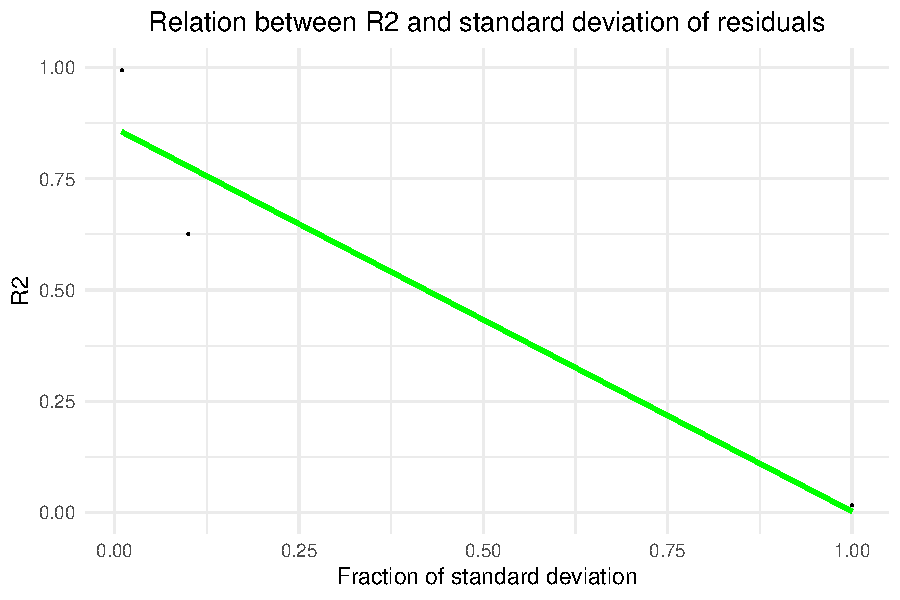
\includegraphics{_main_files/figure-latex/unnamed-chunk-102-1.pdf}
11. {[}Optional{]} Graph \(R^2\) against the standard deviation fraction. Fit a regression line with a polynomial of degree 2. The regression line fits the data better. Is the polynomial regression more informative than the linear regression? Why? What lesson does this graph give you in terms of the importance of understanding the theoretical relations between variables beyond what an empirical approach could suggest? What does it teach you regarding the tension between under- and over-fitting data?

\begin{Shaded}
\begin{Highlighting}[]
\FunctionTok{ggplot}\NormalTok{(table, }\FunctionTok{aes}\NormalTok{(}\AttributeTok{x =}\NormalTok{ SD, }\AttributeTok{y =}\NormalTok{ R2)) }\SpecialCharTok{+}
  \FunctionTok{geom\_point}\NormalTok{() }\SpecialCharTok{+}
  \FunctionTok{geom\_smooth}\NormalTok{(}\AttributeTok{method =} \StringTok{"lm"}\NormalTok{, }\AttributeTok{formula =}\NormalTok{ y }\SpecialCharTok{\textasciitilde{}} \FunctionTok{poly}\NormalTok{(x, }\DecValTok{2}\NormalTok{), }\AttributeTok{se =} \ConstantTok{FALSE}\NormalTok{, }\AttributeTok{color=}\StringTok{\textquotesingle{}green\textquotesingle{}}\NormalTok{) }\SpecialCharTok{+}
  \FunctionTok{theme\_minimal}\NormalTok{() }\SpecialCharTok{+}
  \FunctionTok{theme}\NormalTok{(}\AttributeTok{plot.title =} \FunctionTok{element\_text}\NormalTok{(}\AttributeTok{hjust =} \FloatTok{0.5}\NormalTok{)) }\SpecialCharTok{+}
  \FunctionTok{labs}\NormalTok{(}
    \AttributeTok{x =} \StringTok{"Fraction of standard deviation"}\NormalTok{,}
    \AttributeTok{y =} \StringTok{"R2"}\NormalTok{,}
    \AttributeTok{title =} \StringTok{"Relation between R2 and standard deviation of residuals"}
\NormalTok{  ) }
\end{Highlighting}
\end{Shaded}

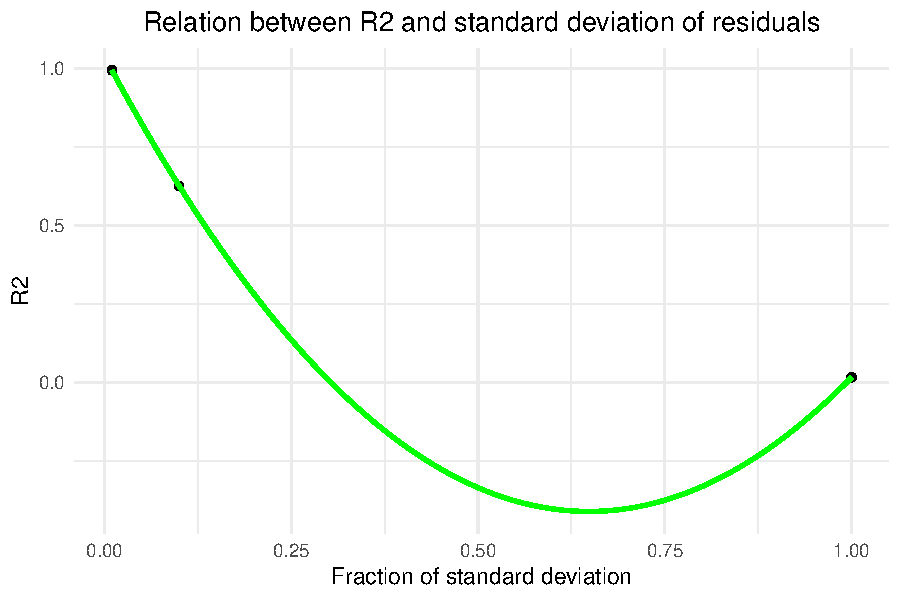
\includegraphics{_main_files/figure-latex/unnamed-chunk-103-1.pdf}
12. Print the parameters generated in the point 1. Generate the same predictions as in point 1 and 2 but this time multiply the slope's parameter by 5, while keeping the intercept unchanged. Call the resulting predictions \texttt{predicted\_LeftToRight\_AdjSlope} Generate a graph with the regression line for \texttt{predicted\_LeftToRight\_AdjSlope} vs \texttt{Age} and compare it with the graph \texttt{predicted\_LeftToRight} vs \texttt{Age} generated in point 1.

Print here

\begin{Shaded}
\begin{Highlighting}[]
\NormalTok{result }\OtherTok{\textless{}{-}} \FunctionTok{lm}\NormalTok{(LeftToRight }\SpecialCharTok{\textasciitilde{}}\NormalTok{ age, }\AttributeTok{data =}\NormalTok{ selects19)}
\CommentTok{\# summary(result)}
\NormalTok{coeffs }\OtherTok{\textless{}{-}} \FunctionTok{coef}\NormalTok{(result)}
\FunctionTok{cat}\NormalTok{(}\StringTok{\textquotesingle{}Intercept:\textquotesingle{}}\NormalTok{,}\FunctionTok{unname}\NormalTok{(coeffs[}\DecValTok{1}\NormalTok{]), }\StringTok{\textquotesingle{}}\SpecialCharTok{\textbackslash{}n\textbackslash{}n}\StringTok{Slope:\textquotesingle{}}\NormalTok{, }\FunctionTok{unname}\NormalTok{(coeffs[}\DecValTok{2}\NormalTok{]))}
\end{Highlighting}
\end{Shaded}

\begin{verbatim}
## Intercept: 4.122055 
## 
## Slope: 0.01948902
\end{verbatim}

Predict with the adjusted slope here.

\begin{Shaded}
\begin{Highlighting}[]
\NormalTok{selects19}\SpecialCharTok{$}\NormalTok{predicted\_LeftToRight\_AdjSlope }\OtherTok{\textless{}{-}} \FunctionTok{unname}\NormalTok{(coeffs[}\DecValTok{1}\NormalTok{])}\SpecialCharTok{+}\NormalTok{(}\FunctionTok{unname}\NormalTok{(coeffs[}\DecValTok{2}\NormalTok{])}\SpecialCharTok{*}\DecValTok{5}\NormalTok{)}\SpecialCharTok{*}\NormalTok{selects19}\SpecialCharTok{$}\NormalTok{age}
\end{Highlighting}
\end{Shaded}

Generate the graph here.

\begin{Shaded}
\begin{Highlighting}[]
\CommentTok{\#Means for Y and X}
\NormalTok{mean\_LeftRight }\OtherTok{\textless{}{-}} \FunctionTok{mean}\NormalTok{(selects19}\SpecialCharTok{$}\NormalTok{predicted\_LeftToRight\_AdjSlope, }\AttributeTok{na.rm =} \ConstantTok{TRUE}\NormalTok{)}
\NormalTok{mean\_age }\OtherTok{\textless{}{-}} \FunctionTok{mean}\NormalTok{(selects19}\SpecialCharTok{$}\NormalTok{age, }\AttributeTok{na.rm =} \ConstantTok{TRUE}\NormalTok{)}

\CommentTok{\# Create a scatter plot}
\FunctionTok{ggplot}\NormalTok{(selects19, }\FunctionTok{aes}\NormalTok{(}\AttributeTok{x =}\NormalTok{ age, }\AttributeTok{y =}\NormalTok{ predicted\_LeftToRight\_AdjSlope)) }\SpecialCharTok{+}
  \FunctionTok{geom\_smooth}\NormalTok{(}\AttributeTok{method =} \StringTok{"lm"}\NormalTok{, }\AttributeTok{formula =}\NormalTok{ y }\SpecialCharTok{\textasciitilde{}}\NormalTok{ x, }\AttributeTok{se =} \ConstantTok{FALSE}\NormalTok{, }\AttributeTok{color =} \StringTok{"red"}\NormalTok{) }\SpecialCharTok{+}  \CommentTok{\# Adding the regression line}
  \FunctionTok{geom\_hline}\NormalTok{(}\AttributeTok{yintercept =}\NormalTok{ mean\_LeftRight, }\AttributeTok{linetype =} \StringTok{"dashed"}\NormalTok{, }\AttributeTok{color =} \StringTok{"green"}\NormalTok{) }\SpecialCharTok{+}  \CommentTok{\# Horizontal line at the mean of y}
  \FunctionTok{geom\_vline}\NormalTok{(}\AttributeTok{xintercept =}\NormalTok{ mean\_age, }\AttributeTok{linetype =} \StringTok{"dashed"}\NormalTok{, }\AttributeTok{color =} \StringTok{"orange"}\NormalTok{) }\SpecialCharTok{+}  \CommentTok{\# Vertical line at the mean of x}
  \FunctionTok{theme\_minimal}\NormalTok{() }\SpecialCharTok{+}
  \FunctionTok{theme}\NormalTok{(}\AttributeTok{plot.title =} \FunctionTok{element\_text}\NormalTok{(}\AttributeTok{hjust =} \FloatTok{0.5}\NormalTok{)) }\SpecialCharTok{+}
  \FunctionTok{scale\_y\_continuous}\NormalTok{(}
    \AttributeTok{limits =} \FunctionTok{c}\NormalTok{(}\DecValTok{0}\NormalTok{, }\DecValTok{15}\NormalTok{),}
    \AttributeTok{breaks =} \FunctionTok{seq}\NormalTok{(}\DecValTok{0}\NormalTok{, }\DecValTok{20}\NormalTok{, }\AttributeTok{by =} \DecValTok{1}\NormalTok{)) }\SpecialCharTok{+}
  \FunctionTok{theme\_minimal}\NormalTok{() }\SpecialCharTok{+}
  \FunctionTok{theme}\NormalTok{(}
    \AttributeTok{plot.title =} \FunctionTok{element\_text}\NormalTok{(}\AttributeTok{hjust =} \FloatTok{0.5}\NormalTok{), }\CommentTok{\# Center the plot title}
    \AttributeTok{panel.grid.major.y =} \FunctionTok{element\_line}\NormalTok{(}\AttributeTok{color =} \StringTok{"grey80"}\NormalTok{, }\AttributeTok{size =} \FloatTok{0.5}\NormalTok{), }\CommentTok{\# Style for major Y grid lines}
    \AttributeTok{panel.grid.minor.y =} \FunctionTok{element\_blank}\NormalTok{() }\CommentTok{\# Remove minor Y grid lines}
\NormalTok{  ) }\SpecialCharTok{+}
  \FunctionTok{labs}\NormalTok{(}
    \AttributeTok{x =} \StringTok{"Age (years)"}\NormalTok{,}
    \AttributeTok{y =} \StringTok{"Political Preferences (left to right)"}\NormalTok{,}
    \AttributeTok{title =} \StringTok{"Scatter plot Age vs. Political Preferences (adj. slope)"}
\NormalTok{  )}
\end{Highlighting}
\end{Shaded}

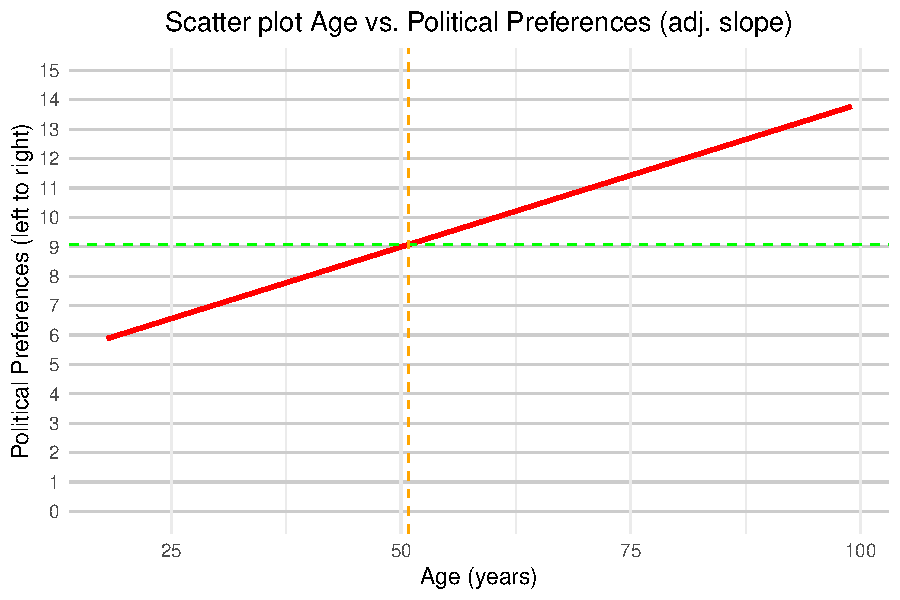
\includegraphics{_main_files/figure-latex/unnamed-chunk-106-1.pdf}
13. Add to the deterministic simulation the same stochastic component generated in point 2. Call that variable \texttt{predicted\_LeftToRight\_AdjSlope\_Stoch}. Generate the graph \texttt{predicted\_LeftToRight\_AdjSlope\_Stoch} vs \texttt{age} with a linear regression line. Generate the \(R^2\) and compare it to the one generated in point 4. Why is the new \(R^2\) higher than the one in point 4?

Report the simulation and the graph here.

\begin{Shaded}
\begin{Highlighting}[]
\NormalTok{selects19}\SpecialCharTok{$}\NormalTok{predicted\_LeftToRight\_AdjSlope\_Stoch }\OtherTok{\textless{}{-}}\NormalTok{ selects19}\SpecialCharTok{$}\NormalTok{predicted\_LeftToRight\_AdjSlope }\SpecialCharTok{+}\NormalTok{ selects19}\SpecialCharTok{$}\NormalTok{NormResiduals1}

\CommentTok{\#Means for Y and X}
\NormalTok{mean\_LeftRight }\OtherTok{\textless{}{-}} \FunctionTok{mean}\NormalTok{(selects19}\SpecialCharTok{$}\NormalTok{predicted\_LeftToRight\_AdjSlope\_Stoch, }\AttributeTok{na.rm =} \ConstantTok{TRUE}\NormalTok{)}
\NormalTok{mean\_age }\OtherTok{\textless{}{-}} \FunctionTok{mean}\NormalTok{(selects19}\SpecialCharTok{$}\NormalTok{age, }\AttributeTok{na.rm =} \ConstantTok{TRUE}\NormalTok{)}

\CommentTok{\# Create a scatter plot}
\FunctionTok{ggplot}\NormalTok{(selects19, }\FunctionTok{aes}\NormalTok{(}\AttributeTok{x =}\NormalTok{ age, }\AttributeTok{y =}\NormalTok{ predicted\_LeftToRight\_AdjSlope\_Stoch)) }\SpecialCharTok{+}
  \FunctionTok{geom\_point}\NormalTok{(}\AttributeTok{size =} \DecValTok{0}\NormalTok{) }\SpecialCharTok{+}
  \FunctionTok{geom\_smooth}\NormalTok{(}\AttributeTok{method =} \StringTok{"lm"}\NormalTok{, }\AttributeTok{formula =}\NormalTok{ y }\SpecialCharTok{\textasciitilde{}}\NormalTok{ x, }\AttributeTok{se =} \ConstantTok{FALSE}\NormalTok{, }\AttributeTok{color =} \StringTok{"red"}\NormalTok{) }\SpecialCharTok{+}  \CommentTok{\# Adding the regression line}
  \FunctionTok{geom\_hline}\NormalTok{(}\AttributeTok{yintercept =}\NormalTok{ mean\_LeftRight, }\AttributeTok{linetype =} \StringTok{"dashed"}\NormalTok{, }\AttributeTok{color =} \StringTok{"green"}\NormalTok{) }\SpecialCharTok{+}  \CommentTok{\# Horizontal line at the mean of y}
  \FunctionTok{geom\_vline}\NormalTok{(}\AttributeTok{xintercept =}\NormalTok{ mean\_age, }\AttributeTok{linetype =} \StringTok{"dashed"}\NormalTok{, }\AttributeTok{color =} \StringTok{"orange"}\NormalTok{) }\SpecialCharTok{+}  \CommentTok{\# Vertical line at the mean of x}
  \FunctionTok{scale\_y\_continuous}\NormalTok{(}
    \AttributeTok{limits =} \FunctionTok{c}\NormalTok{(}\DecValTok{0}\NormalTok{, }\DecValTok{20}\NormalTok{),}
    \AttributeTok{breaks =} \FunctionTok{seq}\NormalTok{(}\DecValTok{0}\NormalTok{, }\DecValTok{20}\NormalTok{, }\AttributeTok{by =} \DecValTok{1}\NormalTok{)) }\SpecialCharTok{+}
  \FunctionTok{theme\_minimal}\NormalTok{() }\SpecialCharTok{+}
  \FunctionTok{theme}\NormalTok{(}
    \AttributeTok{plot.title =} \FunctionTok{element\_text}\NormalTok{(}\AttributeTok{hjust =} \FloatTok{0.5}\NormalTok{), }\CommentTok{\# Center the plot title}
    \AttributeTok{panel.grid.major.y =} \FunctionTok{element\_line}\NormalTok{(}\AttributeTok{color =} \StringTok{"grey80"}\NormalTok{, }\AttributeTok{size =} \FloatTok{0.5}\NormalTok{), }\CommentTok{\# Style for major Y grid lines}
    \AttributeTok{panel.grid.minor.y =} \FunctionTok{element\_blank}\NormalTok{() }\CommentTok{\# Remove minor Y grid lines}
\NormalTok{  ) }\SpecialCharTok{+}
  \FunctionTok{labs}\NormalTok{(}
    \AttributeTok{x =} \StringTok{"Age (years)"}\NormalTok{,}
    \AttributeTok{y =} \StringTok{"Simulation: Political Preferences (left to right)"}\NormalTok{,}
    \AttributeTok{title =} \StringTok{"Scatter plot Age vs. Political Preferences }\SpecialCharTok{\textbackslash{}n}\StringTok{(determ.\& stoch. sim. with adjusted slope)"}
\NormalTok{  )}
\end{Highlighting}
\end{Shaded}

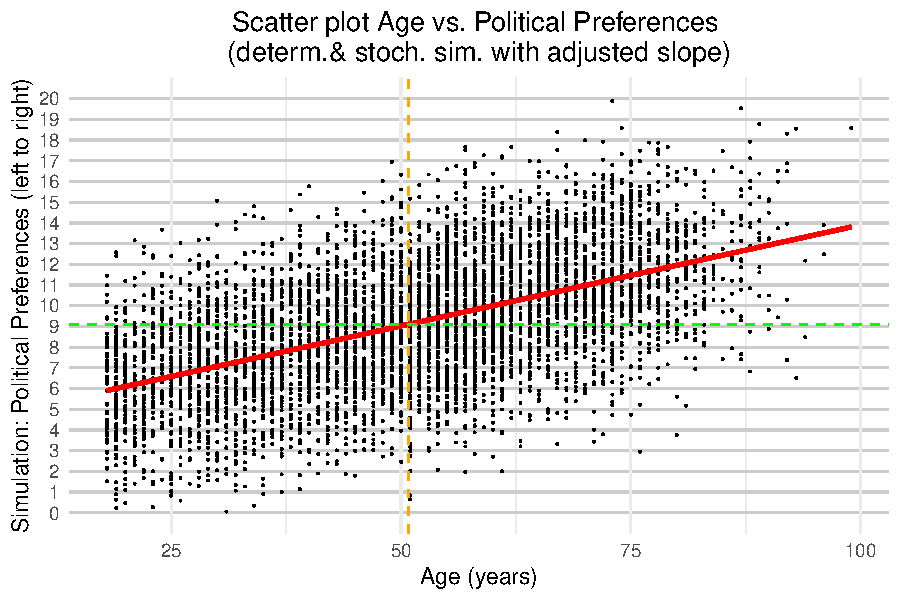
\includegraphics{_main_files/figure-latex/unnamed-chunk-107-1.pdf}

Report the new \(R^2\) here:

\begin{Shaded}
\begin{Highlighting}[]
\NormalTok{result }\OtherTok{\textless{}{-}} \FunctionTok{lm}\NormalTok{(predicted\_LeftToRight\_AdjSlope\_Stoch }\SpecialCharTok{\textasciitilde{}}\NormalTok{ age, }\AttributeTok{data =}\NormalTok{ selects19)}
\NormalTok{rsq\_sd1\_AdjSlope }\OtherTok{\textless{}{-}} \FunctionTok{summary}\NormalTok{(result)}\SpecialCharTok{$}\NormalTok{r.squared}
\FunctionTok{cat}\NormalTok{(}\StringTok{\textquotesingle{}The R2 is: \textquotesingle{}}\NormalTok{, rsq\_sd1\_AdjSlope)}
\end{Highlighting}
\end{Shaded}

\begin{verbatim}
## The R2 is:  0.2973214
\end{verbatim}

Report why is the new \(R^2\) higher than the one in point 4?

\begin{Shaded}
\begin{Highlighting}[]
\FunctionTok{print}\NormalTok{(}\StringTok{\textquotesingle{}The reason the R2 increased is that, while the distance from each observation to the regression line remained unchainged (i.e., the residual was kept unchanged), by increasing the slope of the generating process, the average distance between each observation and the average observation increased (i.e., Y}\SpecialCharTok{\textbackslash{}\textquotesingle{}}\StringTok{s variance increased). See the graph with the red and blue squares mentioned in point 5.\textquotesingle{}}\NormalTok{)}
\end{Highlighting}
\end{Shaded}

\begin{verbatim}
## [1] "The reason the R2 increased is that, while the distance from each observation to the regression line remained unchainged (i.e., the residual was kept unchanged), by increasing the slope of the generating process, the average distance between each observation and the average observation increased (i.e., Y's variance increased). See the graph with the red and blue squares mentioned in point 5."
\end{verbatim}

333333333333

\begin{enumerate}
\def\labelenumi{\arabic{enumi}.}
\setcounter{enumi}{13}
\tightlist
\item
  Print the parameters generated in the point 1. Generate the same predictions as in point 1 and 2 but this time increase in two units the \emph{intercept's} parameter (not the \emph{slope's} parameter as in the point 10), while keeping the slope unchanged. Call the resulting predictions \texttt{predicted\_LeftToRight\_AdjSlope} Generate a graph with the regression line for \texttt{predicted\_LeftToRight\_AdjSlope} vs \texttt{Age} and compare it with the graph \texttt{predicted\_LeftToRight} vs \texttt{Age} generated in point 1.
\end{enumerate}

Print here

\begin{Shaded}
\begin{Highlighting}[]
\NormalTok{result }\OtherTok{\textless{}{-}} \FunctionTok{lm}\NormalTok{(predicted\_LeftToRight\_AdjSlope\_Stoch }\SpecialCharTok{\textasciitilde{}}\NormalTok{ age, }\AttributeTok{data =}\NormalTok{ selects19)}
\CommentTok{\# summary(result)}
\NormalTok{coeffs12 }\OtherTok{\textless{}{-}} \FunctionTok{coef}\NormalTok{(result)}
\FunctionTok{cat}\NormalTok{(}\StringTok{\textquotesingle{}Intercept:\textquotesingle{}}\NormalTok{,}\FunctionTok{unname}\NormalTok{(coeffs12[}\DecValTok{1}\NormalTok{]), }\StringTok{\textquotesingle{}}\SpecialCharTok{\textbackslash{}n\textbackslash{}n}\StringTok{Slope:\textquotesingle{}}\NormalTok{, }\FunctionTok{unname}\NormalTok{(coeffs12[}\DecValTok{2}\NormalTok{]))}
\end{Highlighting}
\end{Shaded}

\begin{verbatim}
## Intercept: 4.071965 
## 
## Slope: 0.09874777
\end{verbatim}

Predict with the adjusted slope here.

\begin{Shaded}
\begin{Highlighting}[]
\NormalTok{selects19}\SpecialCharTok{$}\NormalTok{predicted\_LeftToRight\_AdjIntecept }\OtherTok{\textless{}{-}} \FunctionTok{unname}\NormalTok{(coeffs[}\DecValTok{1}\NormalTok{]}\SpecialCharTok{+}\DecValTok{2}\NormalTok{)}\SpecialCharTok{+}\NormalTok{(}\FunctionTok{unname}\NormalTok{(coeffs[}\DecValTok{2}\NormalTok{]))}\SpecialCharTok{*}\NormalTok{selects19}\SpecialCharTok{$}\NormalTok{age}
\end{Highlighting}
\end{Shaded}

Generate the graph here.

\begin{Shaded}
\begin{Highlighting}[]
\CommentTok{\#Means for Y and X}
\NormalTok{mean\_LeftRight }\OtherTok{\textless{}{-}} \FunctionTok{mean}\NormalTok{(selects19}\SpecialCharTok{$}\NormalTok{predicted\_LeftToRight\_AdjIntecept, }\AttributeTok{na.rm =} \ConstantTok{TRUE}\NormalTok{)}
\NormalTok{mean\_age }\OtherTok{\textless{}{-}} \FunctionTok{mean}\NormalTok{(selects19}\SpecialCharTok{$}\NormalTok{age, }\AttributeTok{na.rm =} \ConstantTok{TRUE}\NormalTok{)}

\CommentTok{\# Create a scatter plot}
\FunctionTok{ggplot}\NormalTok{(selects19, }\FunctionTok{aes}\NormalTok{(}\AttributeTok{x =}\NormalTok{ age, }\AttributeTok{y =}\NormalTok{ predicted\_LeftToRight\_AdjIntecept)) }\SpecialCharTok{+}
  \FunctionTok{geom\_smooth}\NormalTok{(}\AttributeTok{method =} \StringTok{"lm"}\NormalTok{, }\AttributeTok{formula =}\NormalTok{ y }\SpecialCharTok{\textasciitilde{}}\NormalTok{ x, }\AttributeTok{se =} \ConstantTok{FALSE}\NormalTok{, }\AttributeTok{color =} \StringTok{"red"}\NormalTok{) }\SpecialCharTok{+}  \CommentTok{\# Adding the regression line}
  \FunctionTok{geom\_hline}\NormalTok{(}\AttributeTok{yintercept =}\NormalTok{ mean\_LeftRight, }\AttributeTok{linetype =} \StringTok{"dashed"}\NormalTok{, }\AttributeTok{color =} \StringTok{"green"}\NormalTok{) }\SpecialCharTok{+}  \CommentTok{\# Horizontal line at the mean of y}
  \FunctionTok{geom\_vline}\NormalTok{(}\AttributeTok{xintercept =}\NormalTok{ mean\_age, }\AttributeTok{linetype =} \StringTok{"dashed"}\NormalTok{, }\AttributeTok{color =} \StringTok{"orange"}\NormalTok{) }\SpecialCharTok{+}  \CommentTok{\# Vertical line at the mean of x}
  \FunctionTok{theme\_minimal}\NormalTok{() }\SpecialCharTok{+}
  \FunctionTok{theme}\NormalTok{(}\AttributeTok{plot.title =} \FunctionTok{element\_text}\NormalTok{(}\AttributeTok{hjust =} \FloatTok{0.5}\NormalTok{)) }\SpecialCharTok{+}
  \FunctionTok{scale\_y\_continuous}\NormalTok{(}
    \AttributeTok{limits =} \FunctionTok{c}\NormalTok{(}\DecValTok{0}\NormalTok{, }\DecValTok{15}\NormalTok{),}
    \AttributeTok{breaks =} \FunctionTok{seq}\NormalTok{(}\DecValTok{0}\NormalTok{, }\DecValTok{15}\NormalTok{, }\AttributeTok{by =} \DecValTok{1}\NormalTok{)) }\SpecialCharTok{+}
  \FunctionTok{theme\_minimal}\NormalTok{() }\SpecialCharTok{+}
  \FunctionTok{theme}\NormalTok{(}
    \AttributeTok{plot.title =} \FunctionTok{element\_text}\NormalTok{(}\AttributeTok{hjust =} \FloatTok{0.5}\NormalTok{), }\CommentTok{\# Center the plot title}
    \AttributeTok{panel.grid.major.y =} \FunctionTok{element\_line}\NormalTok{(}\AttributeTok{color =} \StringTok{"grey80"}\NormalTok{, }\AttributeTok{size =} \FloatTok{0.5}\NormalTok{), }\CommentTok{\# Style for major Y grid lines}
    \AttributeTok{panel.grid.minor.y =} \FunctionTok{element\_blank}\NormalTok{() }\CommentTok{\# Remove minor Y grid lines}
\NormalTok{  ) }\SpecialCharTok{+}
  \FunctionTok{labs}\NormalTok{(}
    \AttributeTok{x =} \StringTok{"Age (years)"}\NormalTok{,}
    \AttributeTok{y =} \StringTok{"Political Preferences (left to right)"}\NormalTok{,}
    \AttributeTok{title =} \StringTok{"Scatter plot Age vs. Political Preferences (adj. slope)"}
\NormalTok{  )}
\end{Highlighting}
\end{Shaded}

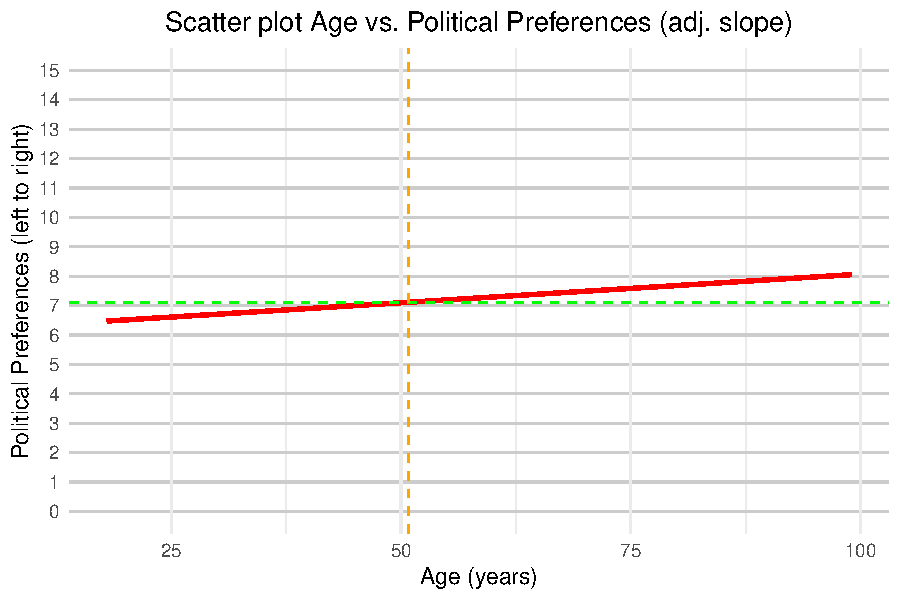
\includegraphics{_main_files/figure-latex/unnamed-chunk-112-1.pdf}
15. Add to the deterministic simulation the same stochastic component generated in point 2. Call that variable \texttt{predicted\_LeftToRight\_AdjIntercep\_Stoch}. Generate the graph \texttt{predicted\_LeftToRight\_AdjIntecept} vs \texttt{age} with a linear regression line. Generate the \(R^2\) and compare it to the one generated in point 4. Why is the new \(R^2\) higher than the one in point 4?

Report the simulation and the graph here.

\begin{Shaded}
\begin{Highlighting}[]
\NormalTok{selects19}\SpecialCharTok{$}\NormalTok{predicted\_LeftToRight\_AdjIntercept\_Stoch }\OtherTok{\textless{}{-}}\NormalTok{ selects19}\SpecialCharTok{$}\NormalTok{predicted\_LeftToRight\_AdjIntecept }\SpecialCharTok{+}\NormalTok{ selects19}\SpecialCharTok{$}\NormalTok{residual}

\CommentTok{\#Means for Y and X}
\NormalTok{mean\_LeftRight }\OtherTok{\textless{}{-}} \FunctionTok{mean}\NormalTok{(selects19}\SpecialCharTok{$}\NormalTok{predicted\_LeftToRight\_AdjIntercept\_Stoch, }\AttributeTok{na.rm =} \ConstantTok{TRUE}\NormalTok{)}
\NormalTok{mean\_age }\OtherTok{\textless{}{-}} \FunctionTok{mean}\NormalTok{(selects19}\SpecialCharTok{$}\NormalTok{age, }\AttributeTok{na.rm =} \ConstantTok{TRUE}\NormalTok{)}

\CommentTok{\# Create a scatter plot}
\FunctionTok{ggplot}\NormalTok{(selects19, }\FunctionTok{aes}\NormalTok{(}\AttributeTok{x =}\NormalTok{ age, }\AttributeTok{y =}\NormalTok{ predicted\_LeftToRight\_AdjIntercept\_Stoch)) }\SpecialCharTok{+}
  \FunctionTok{geom\_point}\NormalTok{(}\AttributeTok{size =} \DecValTok{0}\NormalTok{) }\SpecialCharTok{+}
  \FunctionTok{geom\_smooth}\NormalTok{(}\AttributeTok{method =} \StringTok{"lm"}\NormalTok{, }\AttributeTok{formula =}\NormalTok{ y }\SpecialCharTok{\textasciitilde{}}\NormalTok{ x, }\AttributeTok{se =} \ConstantTok{FALSE}\NormalTok{, }\AttributeTok{color =} \StringTok{"red"}\NormalTok{) }\SpecialCharTok{+}  \CommentTok{\# Adding the regression line}
  \FunctionTok{geom\_hline}\NormalTok{(}\AttributeTok{yintercept =}\NormalTok{ mean\_LeftRight, }\AttributeTok{linetype =} \StringTok{"dashed"}\NormalTok{, }\AttributeTok{color =} \StringTok{"green"}\NormalTok{) }\SpecialCharTok{+}  \CommentTok{\# Horizontal line at the mean of y}
  \FunctionTok{geom\_vline}\NormalTok{(}\AttributeTok{xintercept =}\NormalTok{ mean\_age, }\AttributeTok{linetype =} \StringTok{"dashed"}\NormalTok{, }\AttributeTok{color =} \StringTok{"orange"}\NormalTok{) }\SpecialCharTok{+}  \CommentTok{\# Vertical line at the mean of x}
  \FunctionTok{scale\_y\_continuous}\NormalTok{(}
    \AttributeTok{limits =} \FunctionTok{c}\NormalTok{(}\DecValTok{0}\NormalTok{, }\DecValTok{15}\NormalTok{),}
    \AttributeTok{breaks =} \FunctionTok{seq}\NormalTok{(}\DecValTok{0}\NormalTok{, }\DecValTok{15}\NormalTok{, }\AttributeTok{by =} \DecValTok{1}\NormalTok{)) }\SpecialCharTok{+}
  \FunctionTok{theme\_minimal}\NormalTok{() }\SpecialCharTok{+}
  \FunctionTok{theme}\NormalTok{(}
    \AttributeTok{plot.title =} \FunctionTok{element\_text}\NormalTok{(}\AttributeTok{hjust =} \FloatTok{0.5}\NormalTok{), }\CommentTok{\# Center the plot title}
    \AttributeTok{panel.grid.major.y =} \FunctionTok{element\_line}\NormalTok{(}\AttributeTok{color =} \StringTok{"grey80"}\NormalTok{, }\AttributeTok{size =} \FloatTok{0.5}\NormalTok{), }\CommentTok{\# Style for major Y grid lines}
    \AttributeTok{panel.grid.minor.y =} \FunctionTok{element\_blank}\NormalTok{() }\CommentTok{\# Remove minor Y grid lines}
\NormalTok{  ) }\SpecialCharTok{+}
  \FunctionTok{labs}\NormalTok{(}
    \AttributeTok{x =} \StringTok{"Age (years)"}\NormalTok{,}
    \AttributeTok{y =} \StringTok{"Simulation: Political Preferences (left to right)"}\NormalTok{,}
    \AttributeTok{title =} \StringTok{"Scatter plot Age vs. Political Preferences }\SpecialCharTok{\textbackslash{}n}\StringTok{(determ.\& stoch. sim. with adjusted intercept)"}
\NormalTok{  )}
\end{Highlighting}
\end{Shaded}

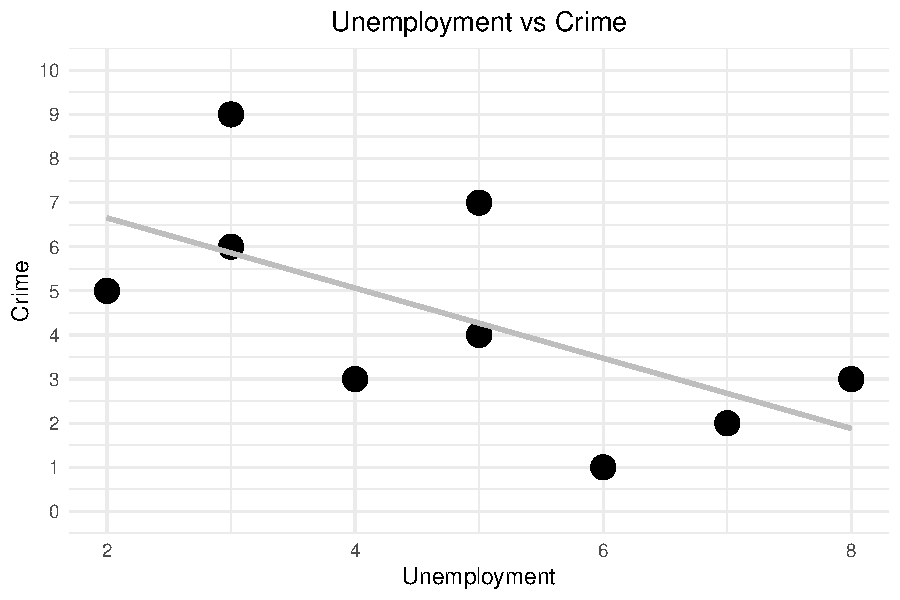
\includegraphics{_main_files/figure-latex/unnamed-chunk-113-1.pdf}
Regress the \texttt{predicted\_LeftToRight\_AdjIntercept\_Stoch} on \texttt{age}

\begin{Shaded}
\begin{Highlighting}[]
\NormalTok{result }\OtherTok{\textless{}{-}} \FunctionTok{lm}\NormalTok{(predicted\_LeftToRight\_AdjIntercept\_Stoch }\SpecialCharTok{\textasciitilde{}}\NormalTok{ age, }\AttributeTok{data =}\NormalTok{ selects19)}
\NormalTok{rsq\_sd1\_AdjIntercept }\OtherTok{\textless{}{-}} \FunctionTok{summary}\NormalTok{(result)}\SpecialCharTok{$}\NormalTok{r.squared}
\NormalTok{coeffs13 }\OtherTok{\textless{}{-}} \FunctionTok{coef}\NormalTok{(result)}
\FunctionTok{cat}\NormalTok{(}\StringTok{\textquotesingle{}Intercept:\textquotesingle{}}\NormalTok{,}\FunctionTok{unname}\NormalTok{(coeffs13[}\DecValTok{1}\NormalTok{]), }\StringTok{\textquotesingle{}}\SpecialCharTok{\textbackslash{}n\textbackslash{}n}\StringTok{Slope:\textquotesingle{}}\NormalTok{, }\FunctionTok{unname}\NormalTok{(coeffs13[}\DecValTok{2}\NormalTok{]))}
\end{Highlighting}
\end{Shaded}

\begin{verbatim}
## Intercept: 6.122055 
## 
## Slope: 0.01948902
\end{verbatim}

Report the \(R^2\) generated in points 2, 11, and 13 here:

\begin{Shaded}
\begin{Highlighting}[]
\NormalTok{tableSD1 }\OtherTok{\textless{}{-}} \FunctionTok{data.frame}\NormalTok{(}
  \AttributeTok{LookR2 =} \FunctionTok{c}\NormalTok{(}\StringTok{\textquotesingle{}Point 2\textquotesingle{}}\NormalTok{, }\StringTok{\textquotesingle{}Point 12\textquotesingle{}}\NormalTok{, }\StringTok{\textquotesingle{}Point 13\textquotesingle{}}\NormalTok{),}
  \AttributeTok{Model =} \FunctionTok{c}\NormalTok{(}\StringTok{\textquotesingle{}Unchanged\textquotesingle{}}\NormalTok{, }\StringTok{\textquotesingle{}P2 + (slope*5)\textquotesingle{}}\NormalTok{, }\StringTok{\textquotesingle{}P2+(intercept+2)\textquotesingle{}}\NormalTok{),}
  \AttributeTok{R2 =} \FunctionTok{c}\NormalTok{(rsq\_sd1, rsq\_sd1\_AdjSlope, rsq\_sd1\_AdjIntercept),    }
  \AttributeTok{LookParams =} \FunctionTok{c}\NormalTok{(}\StringTok{\textquotesingle{}Point 1\textquotesingle{}}\NormalTok{, }\StringTok{\textquotesingle{}Point 12\textquotesingle{}}\NormalTok{, }\StringTok{\textquotesingle{}Point 13\textquotesingle{}}\NormalTok{),}
  \AttributeTok{Intercept =} \FunctionTok{c}\NormalTok{(}\FunctionTok{unname}\NormalTok{(coeffs1[}\DecValTok{1}\NormalTok{]), }\FunctionTok{unname}\NormalTok{(coeffs12[}\DecValTok{1}\NormalTok{]), }\FunctionTok{unname}\NormalTok{(coeffs13[}\DecValTok{1}\NormalTok{])),    }
  \AttributeTok{Slope =} \FunctionTok{c}\NormalTok{(}\FunctionTok{unname}\NormalTok{(coeffs1[}\DecValTok{2}\NormalTok{]), }\FunctionTok{unname}\NormalTok{(coeffs12[}\DecValTok{2}\NormalTok{]), }\FunctionTok{unname}\NormalTok{(coeffs13[}\DecValTok{2}\NormalTok{]))}
\NormalTok{)}


\FunctionTok{print}\NormalTok{(tableSD1)}
\end{Highlighting}
\end{Shaded}

\begin{verbatim}
##     LookR2            Model        R2 LookParams Intercept      Slope
## 1  Point 2        Unchanged 0.0161515    Point 1  4.122055 0.01948902
## 2 Point 12   P2 + (slope*5) 0.2973214   Point 12  4.071965 0.09874777
## 3 Point 13 P2+(intercept+2) 0.0161515   Point 13  6.122055 0.01948902
\end{verbatim}

\begin{enumerate}
\def\labelenumi{\arabic{enumi}.}
\setcounter{enumi}{15}
\tightlist
\item
  Comparing the \(R^2\) and the parameters across the models of points 1, 2, and 3 answer the following questions:
\end{enumerate}

\begin{enumerate}
\def\labelenumi{\roman{enumi}.}
\tightlist
\item
  What effect does increasing the slope of the data generating process (while keeping the residuals and intercept unchanged) have on the \(R^2\)?
\end{enumerate}

\begin{Shaded}
\begin{Highlighting}[]
\FunctionTok{print}\NormalTok{(}\StringTok{\textquotesingle{}The R2 increases as seen in point 13\textquotesingle{}}\NormalTok{)}
\end{Highlighting}
\end{Shaded}

\begin{verbatim}
## [1] "The R2 increases as seen in point 13"
\end{verbatim}

\begin{enumerate}
\def\labelenumi{\roman{enumi}.}
\setcounter{enumi}{1}
\tightlist
\item
  What effect does increasing the intercept of the data generating process (while keeping the residuals and slope unchanged) have on the \(R^2\)?
\end{enumerate}

\begin{Shaded}
\begin{Highlighting}[]
\FunctionTok{print}\NormalTok{(}\StringTok{\textquotesingle{}The R2 stays unchanged as the distance from each observation to the regression line remained unchainged (i.e., the residual was kept unchanged) as well as the average distance between each observation and the average observation remained unchainged (i.e., Y}\SpecialCharTok{\textbackslash{}\textquotesingle{}}\StringTok{s variance was kept unchanged)\textquotesingle{}}\NormalTok{)}
\end{Highlighting}
\end{Shaded}

\begin{verbatim}
## [1] "The R2 stays unchanged as the distance from each observation to the regression line remained unchainged (i.e., the residual was kept unchanged) as well as the average distance between each observation and the average observation remained unchainged (i.e., Y's variance was kept unchanged)"
\end{verbatim}

\begin{enumerate}
\def\labelenumi{\roman{enumi}.}
\setcounter{enumi}{2}
\tightlist
\item
  What effect does increasing the slope of the data generating process (while keeping the residuals and intercept unchanged) have on the intercept and slope?
\end{enumerate}

\begin{Shaded}
\begin{Highlighting}[]
\FunctionTok{print}\NormalTok{(}\StringTok{\textquotesingle{}It increases the estimated slope and decreases the intercept.\textquotesingle{}}\NormalTok{)}
\end{Highlighting}
\end{Shaded}

\begin{verbatim}
## [1] "It increases the estimated slope and decreases the intercept."
\end{verbatim}

\begin{enumerate}
\def\labelenumi{\roman{enumi}.}
\setcounter{enumi}{3}
\tightlist
\item
  What effect does increasing the intercept of the data generating process (while keeping the residuals and slope unchanged) have on the intercept and slope?
\end{enumerate}

\begin{Shaded}
\begin{Highlighting}[]
\FunctionTok{print}\NormalTok{(}\StringTok{\textquotesingle{}It keeps the estimated slope unchanged and the estimated intercept is the same as before the adjustment but increases by the same value that the whole data generating process was modified.\textquotesingle{}}\NormalTok{)}
\end{Highlighting}
\end{Shaded}

\begin{verbatim}
## [1] "It keeps the estimated slope unchanged and the estimated intercept is the same as before the adjustment but increases by the same value that the whole data generating process was modified."
\end{verbatim}

\hypertarget{week-5}{%
\chapter{Week 5}\label{week-5}}

\hypertarget{exercise-1}{%
\section{Exercise}\label{exercise-1}}

\hypertarget{solution-1}{%
\section{Solution}\label{solution-1}}

\hypertarget{week-6}{%
\chapter{Week 6}\label{week-6}}

\hypertarget{exercise-2}{%
\section{Exercise}\label{exercise-2}}

\hypertarget{solution-2}{%
\section{Solution}\label{solution-2}}

\hypertarget{week-7}{%
\chapter{Week 7}\label{week-7}}

\hypertarget{exercise-3}{%
\section{Exercise}\label{exercise-3}}

\hypertarget{solution-3}{%
\section{Solution}\label{solution-3}}

\hypertarget{week-8-causality-iii-observational-data}{%
\chapter{Week 8: Causality III (Observational Data)}\label{week-8-causality-iii-observational-data}}

\hypertarget{aims-3}{%
\section{Aims}\label{aims-3}}

\begin{enumerate}
\def\labelenumi{\arabic{enumi}.}
\tightlist
\item
  Using simulated data to instantiate the logic behind, diff-in-diff and panel data (i.e., within, between, and twoway fixed effects) methods.
\item
  Using real data to estimate a causal effect using a two'way fixed effects model.
\end{enumerate}

\hypertarget{exercise-4}{%
\section{Exercise}\label{exercise-4}}

\hypertarget{simulated-data-2}{%
\subsection{Simulated data}\label{simulated-data-2}}

The following data is NOT real and is inspired by Ben Lambert's video on fixed effects (see \href{https://www.youtube.com/watch?v=1SchyQ77VFg}{here}). It's purpose is simply to illustrate the logic og the fixed effects models.

\begin{Shaded}
\begin{Highlighting}[]
\NormalTok{data }\OtherTok{\textless{}{-}} \FunctionTok{list}\NormalTok{(}
  \AttributeTok{City =} \FunctionTok{c}\NormalTok{(}\StringTok{\textquotesingle{}NYC\textquotesingle{}}\NormalTok{, }\StringTok{\textquotesingle{}NYC\textquotesingle{}}\NormalTok{, }\StringTok{\textquotesingle{}NYC\textquotesingle{}}\NormalTok{, }\StringTok{\textquotesingle{}Boston\textquotesingle{}}\NormalTok{, }\StringTok{\textquotesingle{}Boston\textquotesingle{}}\NormalTok{, }\StringTok{\textquotesingle{}Boston\textquotesingle{}}\NormalTok{, }\StringTok{\textquotesingle{}Amherst\textquotesingle{}}\NormalTok{, }\StringTok{\textquotesingle{}Amherst\textquotesingle{}}\NormalTok{, }\StringTok{\textquotesingle{}Amherst\textquotesingle{}}\NormalTok{),}
  \AttributeTok{Time =} \FunctionTok{c}\NormalTok{(}\DecValTok{1}\NormalTok{, }\DecValTok{2}\NormalTok{, }\DecValTok{3}\NormalTok{, }\DecValTok{1}\NormalTok{, }\DecValTok{2}\NormalTok{, }\DecValTok{3}\NormalTok{, }\DecValTok{1}\NormalTok{, }\DecValTok{2}\NormalTok{, }\DecValTok{3}\NormalTok{),}
  \AttributeTok{Unemployment =} \FunctionTok{c}\NormalTok{(}\DecValTok{2}\NormalTok{, }\DecValTok{3}\NormalTok{, }\DecValTok{3}\NormalTok{, }\DecValTok{4}\NormalTok{, }\DecValTok{5}\NormalTok{, }\DecValTok{5}\NormalTok{, }\DecValTok{6}\NormalTok{, }\DecValTok{7}\NormalTok{, }\DecValTok{8}\NormalTok{),}
  \AttributeTok{Crime =} \FunctionTok{c}\NormalTok{(}\DecValTok{5}\NormalTok{, }\DecValTok{6}\NormalTok{, }\DecValTok{9}\NormalTok{, }\DecValTok{3}\NormalTok{, }\DecValTok{4}\NormalTok{, }\DecValTok{7}\NormalTok{, }\DecValTok{1}\NormalTok{, }\DecValTok{2}\NormalTok{, }\DecValTok{3}\NormalTok{),}
  \AttributeTok{Treatment =} \FunctionTok{c}\NormalTok{(}\DecValTok{0}\NormalTok{, }\DecValTok{0}\NormalTok{, }\DecValTok{1}\NormalTok{, }\DecValTok{0}\NormalTok{, }\DecValTok{0}\NormalTok{, }\DecValTok{1}\NormalTok{, }\DecValTok{0}\NormalTok{, }\DecValTok{0}\NormalTok{, }\DecValTok{0}\NormalTok{)}
\NormalTok{)}

\NormalTok{df }\OtherTok{\textless{}{-}} \FunctionTok{data.frame}\NormalTok{(data)}

\CommentTok{\# Overall averages}
\NormalTok{df }\OtherTok{\textless{}{-}}\NormalTok{ df }\SpecialCharTok{\%\textgreater{}\%}
  \FunctionTok{mutate}\NormalTok{(}\AttributeTok{Y\_OverallAverage =} \FunctionTok{mean}\NormalTok{(Crime),}
         \AttributeTok{X\_OverallAverage =} \FunctionTok{mean}\NormalTok{(Unemployment))}

\CommentTok{\# Within averages         }
\NormalTok{df }\OtherTok{\textless{}{-}}\NormalTok{ df }\SpecialCharTok{\%\textgreater{}\%}
  \FunctionTok{group\_by}\NormalTok{(City) }\SpecialCharTok{\%\textgreater{}\%}
  \FunctionTok{mutate}\NormalTok{(}\AttributeTok{Y\_WithinAverage =} \FunctionTok{mean}\NormalTok{(Crime), }
         \AttributeTok{X\_WithinAverage =} \FunctionTok{mean}\NormalTok{(Unemployment))       }

\CommentTok{\# Between averages}
\NormalTok{df }\OtherTok{\textless{}{-}}\NormalTok{ df }\SpecialCharTok{\%\textgreater{}\%}
  \FunctionTok{group\_by}\NormalTok{(Time) }\SpecialCharTok{\%\textgreater{}\%}
  \FunctionTok{mutate}\NormalTok{(}\AttributeTok{Y\_BetweenAverage =} \FunctionTok{mean}\NormalTok{(Crime), }
         \AttributeTok{X\_BetweenAverage =} \FunctionTok{mean}\NormalTok{(Unemployment))}
         
\NormalTok{df}\OtherTok{\textless{}{-}}\NormalTok{ df }\SpecialCharTok{\%\textgreater{}\%}
  \FunctionTok{mutate}\NormalTok{( }\AttributeTok{Y\_demeaned\_within =}\NormalTok{ Crime}\SpecialCharTok{{-}}\NormalTok{Y\_WithinAverage,}
          \AttributeTok{Y\_demeaned\_between =}\NormalTok{ Crime}\SpecialCharTok{{-}}\NormalTok{Y\_BetweenAverage,}
          \AttributeTok{Y\_double\_demeaned =}\NormalTok{ Crime}\SpecialCharTok{{-}}\NormalTok{Y\_WithinAverage}\SpecialCharTok{{-}}\NormalTok{Y\_BetweenAverage}\SpecialCharTok{+}\NormalTok{Y\_OverallAverage,}
          \AttributeTok{X\_demeaned\_within =}\NormalTok{ Unemployment}\SpecialCharTok{{-}}\NormalTok{X\_WithinAverage,}
          \AttributeTok{X\_demeaned\_between =}\NormalTok{ Unemployment}\SpecialCharTok{{-}}\NormalTok{X\_BetweenAverage,}
          \AttributeTok{X\_double\_demeaned =}\NormalTok{ Unemployment}\SpecialCharTok{{-}}\NormalTok{X\_WithinAverage}\SpecialCharTok{{-}}\NormalTok{X\_BetweenAverage}\SpecialCharTok{+}\NormalTok{X\_OverallAverage}
\NormalTok{        )}
\end{Highlighting}
\end{Shaded}

First the basic graph

\begin{Shaded}
\begin{Highlighting}[]
\FunctionTok{ggplot}\NormalTok{(df, }\FunctionTok{aes}\NormalTok{(}\AttributeTok{x =}\NormalTok{ Unemployment, }\AttributeTok{y =}\NormalTok{ Crime)) }\SpecialCharTok{+}
  \FunctionTok{geom\_point}\NormalTok{(}\AttributeTok{size =} \DecValTok{5}\NormalTok{) }\SpecialCharTok{+}
  \FunctionTok{geom\_smooth}\NormalTok{(}\AttributeTok{method =} \StringTok{"lm"}\NormalTok{, }\AttributeTok{formula =}\NormalTok{ y }\SpecialCharTok{\textasciitilde{}}\NormalTok{ x, }\AttributeTok{se =} \ConstantTok{FALSE}\NormalTok{, }\AttributeTok{color =} \StringTok{"gray"}\NormalTok{) }\SpecialCharTok{+}  \CommentTok{\# Adding the regression line}

  \FunctionTok{scale\_y\_continuous}\NormalTok{(}
    \AttributeTok{limits =} \FunctionTok{c}\NormalTok{(}\DecValTok{0}\NormalTok{, }\DecValTok{10}\NormalTok{),}
    \AttributeTok{breaks =} \FunctionTok{seq}\NormalTok{(}\DecValTok{0}\NormalTok{, }\DecValTok{10}\NormalTok{, }\AttributeTok{by =} \DecValTok{1}\NormalTok{)) }\SpecialCharTok{+}
  \FunctionTok{theme\_minimal}\NormalTok{()}\SpecialCharTok{+}
  \FunctionTok{theme}\NormalTok{(}\AttributeTok{plot.title =} \FunctionTok{element\_text}\NormalTok{(}\AttributeTok{hjust =} \FloatTok{0.5}\NormalTok{)) }\SpecialCharTok{+}
  \FunctionTok{labs}\NormalTok{(}\AttributeTok{title =} \StringTok{"Unemployment vs Crime"}\NormalTok{,}
       \AttributeTok{x =} \StringTok{"Unemployment"}\NormalTok{,}
       \AttributeTok{y =} \StringTok{"Crime"}
\NormalTok{       )}
\end{Highlighting}
\end{Shaded}

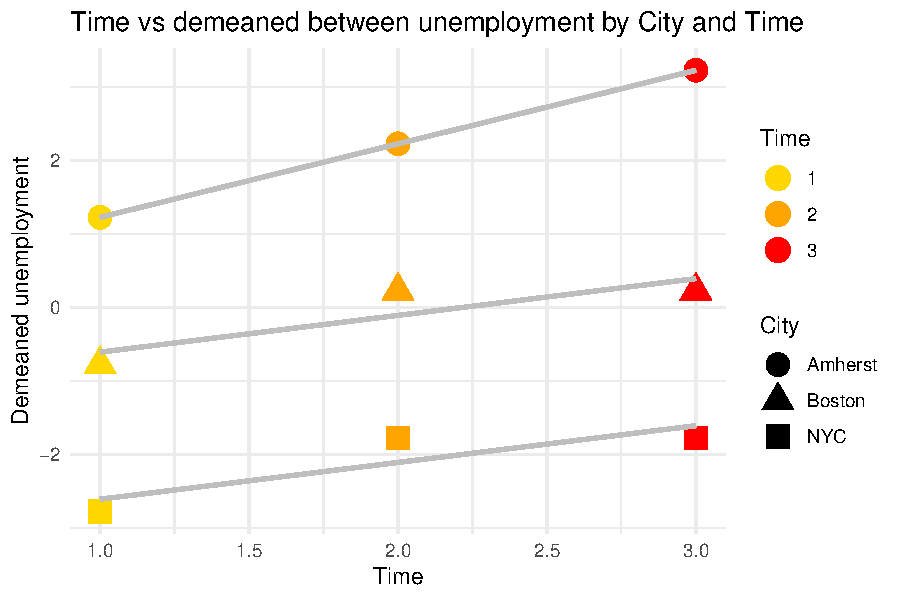
\includegraphics{_main_files/figure-latex/unnamed-chunk-122-1.pdf}

Now use shapes for distinguishing cities.

\begin{Shaded}
\begin{Highlighting}[]
\FunctionTok{ggplot}\NormalTok{(df, }\FunctionTok{aes}\NormalTok{(}\AttributeTok{x =}\NormalTok{ Unemployment, }\AttributeTok{y =}\NormalTok{ Crime)) }\SpecialCharTok{+}
  \FunctionTok{geom\_point}\NormalTok{(}\FunctionTok{aes}\NormalTok{(}\AttributeTok{shape =} \FunctionTok{factor}\NormalTok{(City)), }\AttributeTok{size =} \DecValTok{5}\NormalTok{) }\SpecialCharTok{+}  \CommentTok{\# Apply shape by City only to points}
  \FunctionTok{geom\_smooth}\NormalTok{(}\AttributeTok{method =} \StringTok{"lm"}\NormalTok{, }\AttributeTok{formula =}\NormalTok{ y }\SpecialCharTok{\textasciitilde{}}\NormalTok{ x, }\AttributeTok{se =} \ConstantTok{FALSE}\NormalTok{, }\AttributeTok{color =} \StringTok{"gray"}\NormalTok{) }\SpecialCharTok{+}  \CommentTok{\# Regression line for all data}
  \FunctionTok{scale\_y\_continuous}\NormalTok{(}
    \AttributeTok{limits =} \FunctionTok{c}\NormalTok{(}\DecValTok{0}\NormalTok{, }\DecValTok{10}\NormalTok{),}
    \AttributeTok{breaks =} \FunctionTok{seq}\NormalTok{(}\DecValTok{0}\NormalTok{, }\DecValTok{10}\NormalTok{, }\AttributeTok{by =} \DecValTok{1}\NormalTok{)) }\SpecialCharTok{+}
  \FunctionTok{theme\_minimal}\NormalTok{() }\SpecialCharTok{+}
  \FunctionTok{theme}\NormalTok{(}\AttributeTok{plot.title =} \FunctionTok{element\_text}\NormalTok{(}\AttributeTok{hjust =} \FloatTok{0.5}\NormalTok{)) }\SpecialCharTok{+}
  \FunctionTok{labs}\NormalTok{(}\AttributeTok{title =} \StringTok{"Unemployment vs Crime by City and Time"}\NormalTok{,}
       \AttributeTok{x =} \StringTok{"Unemployment"}\NormalTok{,}
       \AttributeTok{y =} \StringTok{"Crime"}\NormalTok{,}
       \AttributeTok{shape =} \StringTok{"City"}\NormalTok{)}
\end{Highlighting}
\end{Shaded}

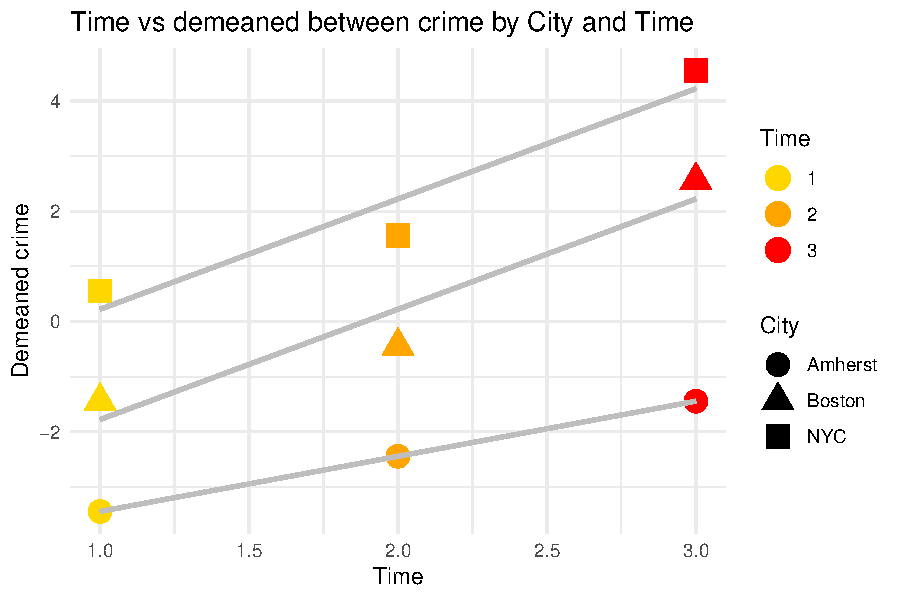
\includegraphics{_main_files/figure-latex/unnamed-chunk-123-1.pdf}

Now also use color for distinguishing also periods.

\begin{Shaded}
\begin{Highlighting}[]
\FunctionTok{ggplot}\NormalTok{(df, }\FunctionTok{aes}\NormalTok{(}\AttributeTok{x =}\NormalTok{ Unemployment, }\AttributeTok{y =}\NormalTok{ Crime)) }\SpecialCharTok{+}
  \FunctionTok{geom\_point}\NormalTok{(}\FunctionTok{aes}\NormalTok{(}\AttributeTok{shape =} \FunctionTok{factor}\NormalTok{(City), }\AttributeTok{color =} \FunctionTok{factor}\NormalTok{(Time)), }\AttributeTok{size =} \DecValTok{5}\NormalTok{) }\SpecialCharTok{+}  \CommentTok{\# Apply shape by City only to points}
  \FunctionTok{scale\_color\_manual}\NormalTok{(}\AttributeTok{values =} \FunctionTok{c}\NormalTok{(}\StringTok{"gold"}\NormalTok{, }\StringTok{"orange"}\NormalTok{, }\StringTok{"red"}\NormalTok{)) }\SpecialCharTok{+}
  \FunctionTok{geom\_smooth}\NormalTok{(}\AttributeTok{method =} \StringTok{"lm"}\NormalTok{, }\AttributeTok{formula =}\NormalTok{ y }\SpecialCharTok{\textasciitilde{}}\NormalTok{ x, }\AttributeTok{se =} \ConstantTok{FALSE}\NormalTok{, }\AttributeTok{color =} \StringTok{"gray"}\NormalTok{) }\SpecialCharTok{+}  \CommentTok{\# Regression line for all data}
  \FunctionTok{scale\_y\_continuous}\NormalTok{(}
    \AttributeTok{limits =} \FunctionTok{c}\NormalTok{(}\DecValTok{0}\NormalTok{, }\DecValTok{10}\NormalTok{),}
    \AttributeTok{breaks =} \FunctionTok{seq}\NormalTok{(}\DecValTok{0}\NormalTok{, }\DecValTok{10}\NormalTok{, }\AttributeTok{by =} \DecValTok{1}\NormalTok{)) }\SpecialCharTok{+}
  \FunctionTok{theme\_minimal}\NormalTok{() }\SpecialCharTok{+}
  \FunctionTok{theme}\NormalTok{(}\AttributeTok{plot.title =} \FunctionTok{element\_text}\NormalTok{(}\AttributeTok{hjust =} \FloatTok{0.5}\NormalTok{)) }\SpecialCharTok{+}
  \FunctionTok{labs}\NormalTok{(}\AttributeTok{title =} \StringTok{"Unemployment vs Crime by City and Time"}\NormalTok{,}
       \AttributeTok{x =} \StringTok{"Unemployment"}\NormalTok{,}
       \AttributeTok{y =} \StringTok{"Crime"}\NormalTok{,}
       \AttributeTok{color =} \StringTok{"Time"}\NormalTok{,}
       \AttributeTok{shape =} \StringTok{"City"}\NormalTok{)}
\end{Highlighting}
\end{Shaded}

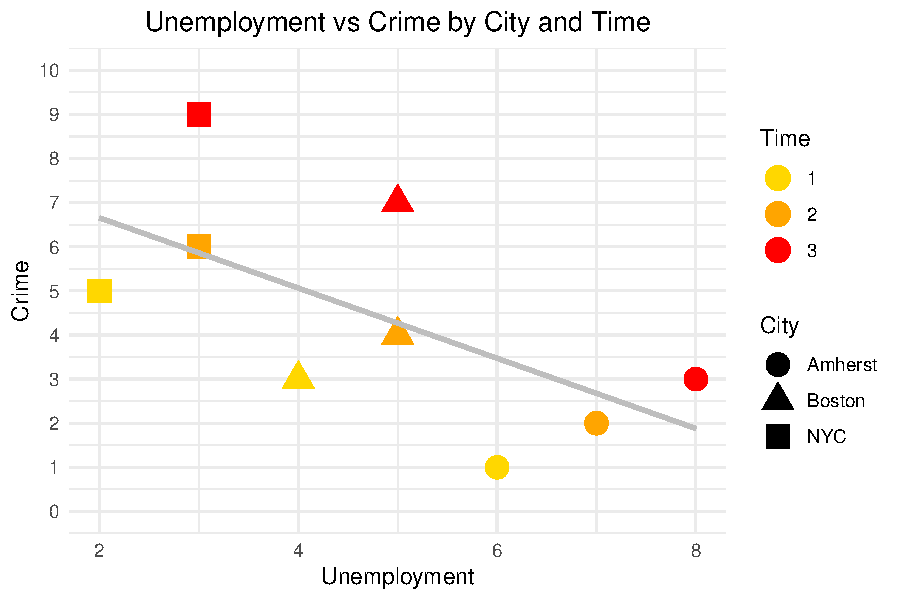
\includegraphics{_main_files/figure-latex/unnamed-chunk-124-1.pdf}

All previous regressions are counter intuitive, why?. Now restrict the regression to each city. What does this suggest regarding the ability of linear regression to capture relations between our variables of interest this scenario? Can we use a regression regardless of how we frame it? Is theory important for guiding how the regression is used? If so, in this case, how?

\begin{Shaded}
\begin{Highlighting}[]
\FunctionTok{ggplot}\NormalTok{(df, }\FunctionTok{aes}\NormalTok{(}\AttributeTok{x =}\NormalTok{ Unemployment, }\AttributeTok{y =}\NormalTok{ Crime, }\AttributeTok{color =} \FunctionTok{factor}\NormalTok{(Time), }\AttributeTok{shape =} \FunctionTok{factor}\NormalTok{(City))) }\SpecialCharTok{+}
  \FunctionTok{geom\_point}\NormalTok{(}\AttributeTok{size =} \DecValTok{5}\NormalTok{) }\SpecialCharTok{+}
  \FunctionTok{scale\_color\_manual}\NormalTok{(}\AttributeTok{values =} \FunctionTok{c}\NormalTok{(}\StringTok{"gold"}\NormalTok{, }\StringTok{"orange"}\NormalTok{, }\StringTok{"red"}\NormalTok{)) }\SpecialCharTok{+}
  \FunctionTok{geom\_smooth}\NormalTok{(}\AttributeTok{method =} \StringTok{"lm"}\NormalTok{, }\AttributeTok{formula =}\NormalTok{ y }\SpecialCharTok{\textasciitilde{}}\NormalTok{ x, }\AttributeTok{se =} \ConstantTok{FALSE}\NormalTok{, }\AttributeTok{color =} \StringTok{"gray"}\NormalTok{) }\SpecialCharTok{+}  \CommentTok{\# Adding the regression line}

  \FunctionTok{scale\_y\_continuous}\NormalTok{(}
  \AttributeTok{limits =} \FunctionTok{c}\NormalTok{(}\DecValTok{0}\NormalTok{, }\DecValTok{10}\NormalTok{),}
  \AttributeTok{breaks =} \FunctionTok{seq}\NormalTok{(}\DecValTok{0}\NormalTok{, }\DecValTok{10}\NormalTok{, }\AttributeTok{by =} \DecValTok{1}\NormalTok{)) }\SpecialCharTok{+}
  
  \FunctionTok{labs}\NormalTok{(}\AttributeTok{title =} \StringTok{"Unemployment vs Crime by City and Time"}\NormalTok{,}
       \AttributeTok{x =} \StringTok{"Unemployment"}\NormalTok{,}
       \AttributeTok{y =} \StringTok{"Crime"}\NormalTok{,}
       \AttributeTok{color =} \StringTok{"Time"}\NormalTok{,}
       \AttributeTok{shape =} \StringTok{"City"}\NormalTok{) }\SpecialCharTok{+}
  \FunctionTok{theme\_minimal}\NormalTok{()}
\end{Highlighting}
\end{Shaded}

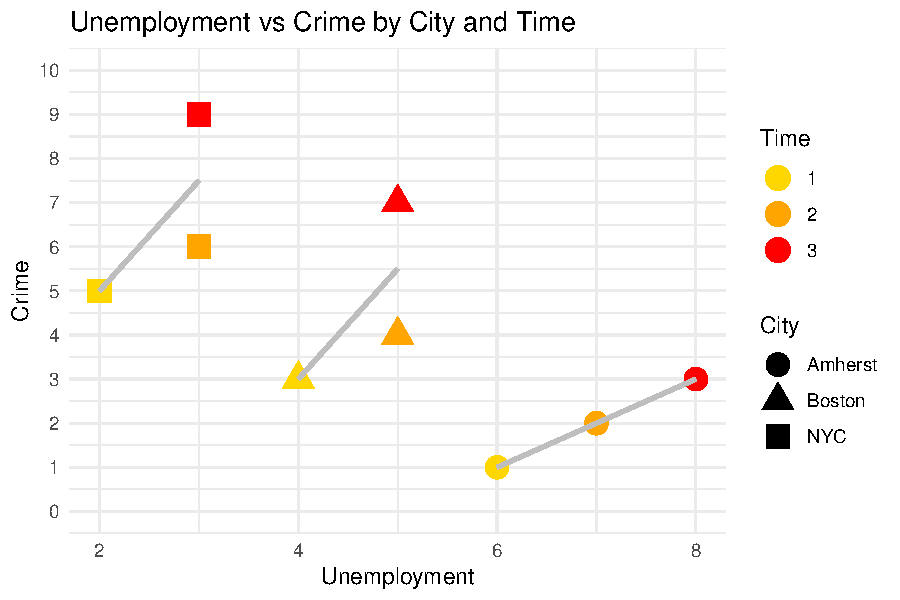
\includegraphics{_main_files/figure-latex/unnamed-chunk-125-1.pdf}

Now, having seen how regressions are theory dependent for defining how they are framed, let's see how fixed effects work.

Assume that the data generating process behind the relation between \texttt{unemployment} and \texttt{crime} is given by the following formula.

\[Y_{it}=\alpha_{i}+\beta_{t}+\gamma_{it}X_{it}+\epsilon_{it}\]
With \[t=1, ..., T\]
and
\[i=1, ..., N\]

Where \(Y_{it}\) is \texttt{crime} for city \(i\) at time \(t\), \(\alpha_{i}\) is a time invariant unobservable (or unobserved) factor influencing the levels of \texttt{crime} in city \(i\) (i.e., it's influence is constant across all periods). \(\beta_{t}\) is a city invariant unobservable (or unobserved) factor influencing the levels of \texttt{crime} at period \(t\) (i.e., it's influence is constant across all cities). \(\gamma_{it}\) is the marginal effect of \(X_{it}\), the \texttt{unemployment} level at city \(i\) in period \(t\). Finally, \(\epsilon_{it}\) is the residual for city \(i\) in period \(t\)

Thus, in order to get rid of the time invariant factor, we can implement the following transformation.

\(\bar{X}_{i.} = \frac{1}{T}*sum_{t=1}^{T} X_{it}.\)

{perhaps showing only the within case is enough? I'm considering to use \textbf{\href{https://economics.princeton.edu/wp-content/uploads/2021/08/two_way_mundlak-Wooldridge.pdf}{this}} paper, particularly page 8.}

Plus vertical line for within mean values.

\begin{Shaded}
\begin{Highlighting}[]
\NormalTok{X\_WithinAverage\_NYC }\OtherTok{=}\NormalTok{ df}\SpecialCharTok{$}\NormalTok{X\_WithinAverage[df}\SpecialCharTok{$}\NormalTok{City}\SpecialCharTok{==}\StringTok{\textquotesingle{}NYC\textquotesingle{}}\NormalTok{][}\DecValTok{1}\NormalTok{]}
\NormalTok{X\_WithinAverage\_Boston }\OtherTok{=}\NormalTok{ df}\SpecialCharTok{$}\NormalTok{X\_WithinAverage[df}\SpecialCharTok{$}\NormalTok{City}\SpecialCharTok{==}\StringTok{\textquotesingle{}Boston\textquotesingle{}}\NormalTok{][}\DecValTok{1}\NormalTok{]}
\NormalTok{X\_WithinAverage\_Amherst }\OtherTok{=}\NormalTok{ df}\SpecialCharTok{$}\NormalTok{X\_WithinAverage[df}\SpecialCharTok{$}\NormalTok{City}\SpecialCharTok{==}\StringTok{\textquotesingle{}Amherst\textquotesingle{}}\NormalTok{][}\DecValTok{1}\NormalTok{]}


\FunctionTok{ggplot}\NormalTok{(df, }\FunctionTok{aes}\NormalTok{(}\AttributeTok{x =}\NormalTok{ Unemployment, }\AttributeTok{y =}\NormalTok{ Crime, }\AttributeTok{color =} \FunctionTok{factor}\NormalTok{(Time), }\AttributeTok{shape =} \FunctionTok{factor}\NormalTok{(City))) }\SpecialCharTok{+}
  \FunctionTok{geom\_point}\NormalTok{(}\AttributeTok{size =} \DecValTok{5}\NormalTok{) }\SpecialCharTok{+}
  \FunctionTok{scale\_color\_manual}\NormalTok{(}\AttributeTok{values =} \FunctionTok{c}\NormalTok{(}\StringTok{"gold"}\NormalTok{, }\StringTok{"orange"}\NormalTok{, }\StringTok{"red"}\NormalTok{)) }\SpecialCharTok{+}
  \FunctionTok{geom\_smooth}\NormalTok{(}\AttributeTok{method =} \StringTok{"lm"}\NormalTok{, }\AttributeTok{formula =}\NormalTok{ y }\SpecialCharTok{\textasciitilde{}}\NormalTok{ x, }\AttributeTok{se =} \ConstantTok{FALSE}\NormalTok{, }\AttributeTok{color =} \StringTok{"gray"}\NormalTok{) }\SpecialCharTok{+}  \CommentTok{\# Adding the regression line}
  \FunctionTok{geom\_vline}\NormalTok{(}\AttributeTok{xintercept =}\NormalTok{ X\_WithinAverage\_NYC, }\AttributeTok{linetype =} \StringTok{"dashed"}\NormalTok{, }\AttributeTok{color =} \StringTok{"lightgray"}\NormalTok{) }\SpecialCharTok{+}  \CommentTok{\# Vertical line at the mean of}
  \FunctionTok{geom\_vline}\NormalTok{(}\AttributeTok{xintercept =}\NormalTok{ X\_WithinAverage\_Boston, }\AttributeTok{linetype =} \StringTok{"dashed"}\NormalTok{, }\AttributeTok{color =} \StringTok{"lightgray"}\NormalTok{) }\SpecialCharTok{+}  \CommentTok{\# Vertical line at the mean of}
  \FunctionTok{geom\_vline}\NormalTok{(}\AttributeTok{xintercept =}\NormalTok{ X\_WithinAverage\_Amherst, }\AttributeTok{linetype =} \StringTok{"dashed"}\NormalTok{, }\AttributeTok{color =} \StringTok{"lightgray"}\NormalTok{) }\SpecialCharTok{+}  \CommentTok{\# Vertical line at the mean of}
  \FunctionTok{scale\_y\_continuous}\NormalTok{(}
  \AttributeTok{limits =} \FunctionTok{c}\NormalTok{(}\DecValTok{0}\NormalTok{, }\DecValTok{10}\NormalTok{),}
  \AttributeTok{breaks =} \FunctionTok{seq}\NormalTok{(}\DecValTok{0}\NormalTok{, }\DecValTok{10}\NormalTok{, }\AttributeTok{by =} \DecValTok{1}\NormalTok{)) }\SpecialCharTok{+}
  
  \FunctionTok{labs}\NormalTok{(}\AttributeTok{title =} \StringTok{"Unemployment vs Crime by City and Time"}\NormalTok{,}
       \AttributeTok{x =} \StringTok{"Unemployment"}\NormalTok{,}
       \AttributeTok{y =} \StringTok{"Crime"}\NormalTok{,}
       \AttributeTok{color =} \StringTok{"Time"}\NormalTok{,}
       \AttributeTok{shape =} \StringTok{"City"}\NormalTok{) }\SpecialCharTok{+}
  \FunctionTok{theme\_minimal}\NormalTok{()}
\end{Highlighting}
\end{Shaded}

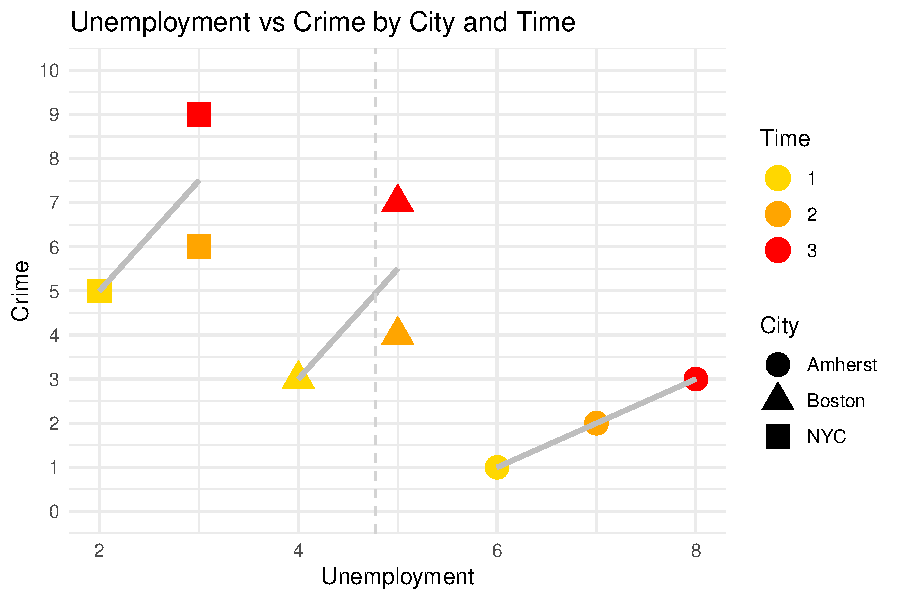
\includegraphics{_main_files/figure-latex/unnamed-chunk-126-1.pdf}

Demeaned within unemployment.

\begin{Shaded}
\begin{Highlighting}[]
\FunctionTok{ggplot}\NormalTok{(df, }\FunctionTok{aes}\NormalTok{(}\AttributeTok{x =}\NormalTok{ X\_demeaned\_within, }\AttributeTok{y =}\NormalTok{ Crime, }\AttributeTok{color =} \FunctionTok{factor}\NormalTok{(Time), }\AttributeTok{shape =} \FunctionTok{factor}\NormalTok{(City))) }\SpecialCharTok{+}
  \FunctionTok{geom\_point}\NormalTok{(}\AttributeTok{size =} \DecValTok{5}\NormalTok{) }\SpecialCharTok{+}
  \FunctionTok{scale\_color\_manual}\NormalTok{(}\AttributeTok{values =} \FunctionTok{c}\NormalTok{(}\StringTok{"gold"}\NormalTok{, }\StringTok{"orange"}\NormalTok{, }\StringTok{"red"}\NormalTok{)) }\SpecialCharTok{+}
  \FunctionTok{geom\_smooth}\NormalTok{(}\AttributeTok{method =} \StringTok{"lm"}\NormalTok{, }\AttributeTok{formula =}\NormalTok{ y }\SpecialCharTok{\textasciitilde{}}\NormalTok{ x, }\AttributeTok{se =} \ConstantTok{FALSE}\NormalTok{, }\AttributeTok{color =} \StringTok{"gray"}\NormalTok{) }\SpecialCharTok{+}  \CommentTok{\# Adding the regression line}
  \FunctionTok{scale\_y\_continuous}\NormalTok{(}
  \AttributeTok{limits =} \FunctionTok{c}\NormalTok{(}\DecValTok{0}\NormalTok{, }\DecValTok{10}\NormalTok{),}
  \AttributeTok{breaks =} \FunctionTok{seq}\NormalTok{(}\DecValTok{0}\NormalTok{, }\DecValTok{10}\NormalTok{, }\AttributeTok{by =} \DecValTok{1}\NormalTok{)) }\SpecialCharTok{+}
  
  \FunctionTok{labs}\NormalTok{(}\AttributeTok{title =} \StringTok{"Demeaned within unemployment vs Crime by City and Time"}\NormalTok{,}
       \AttributeTok{x =} \StringTok{"Demeaned unemployment"}\NormalTok{,}
       \AttributeTok{y =} \StringTok{"Crime"}\NormalTok{,}
       \AttributeTok{color =} \StringTok{"Time"}\NormalTok{,}
       \AttributeTok{shape =} \StringTok{"City"}\NormalTok{) }\SpecialCharTok{+}
  \FunctionTok{theme\_minimal}\NormalTok{()}
\end{Highlighting}
\end{Shaded}

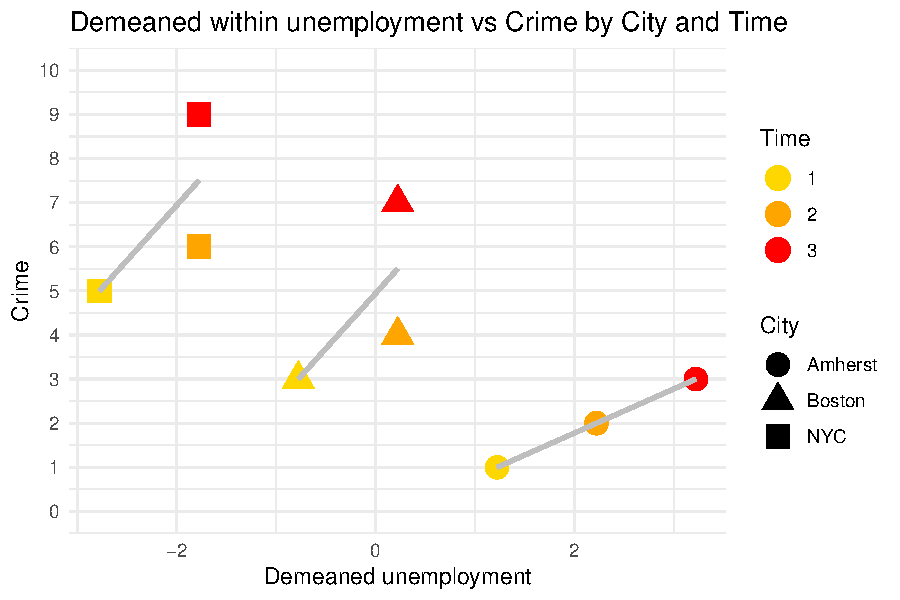
\includegraphics{_main_files/figure-latex/unnamed-chunk-127-1.pdf}

Also demeaned within crime.

\begin{Shaded}
\begin{Highlighting}[]
\FunctionTok{ggplot}\NormalTok{(df, }\FunctionTok{aes}\NormalTok{(}\AttributeTok{x =}\NormalTok{ X\_demeaned\_within, }\AttributeTok{y =}\NormalTok{ Y\_demeaned\_within)) }\SpecialCharTok{+}
  \FunctionTok{geom\_point}\NormalTok{(}\FunctionTok{aes}\NormalTok{(}\AttributeTok{shape =} \FunctionTok{factor}\NormalTok{(City), }\AttributeTok{color =} \FunctionTok{factor}\NormalTok{(Time)), }\AttributeTok{size =} \DecValTok{5}\NormalTok{) }\SpecialCharTok{+}
  \FunctionTok{scale\_color\_manual}\NormalTok{(}\AttributeTok{values =} \FunctionTok{c}\NormalTok{(}\StringTok{"gold"}\NormalTok{, }\StringTok{"orange"}\NormalTok{, }\StringTok{"red"}\NormalTok{)) }\SpecialCharTok{+}
  \FunctionTok{geom\_smooth}\NormalTok{(}\AttributeTok{method =} \StringTok{"lm"}\NormalTok{, }\AttributeTok{formula =}\NormalTok{ y }\SpecialCharTok{\textasciitilde{}}\NormalTok{ x, }\AttributeTok{se =} \ConstantTok{FALSE}\NormalTok{, }\AttributeTok{color =} \StringTok{"gray"}\NormalTok{) }\SpecialCharTok{+}  \CommentTok{\# Adding the regression line}

  \FunctionTok{labs}\NormalTok{(}\AttributeTok{title =} \StringTok{"Demeaned unemployment vs Demeaned crime by City and Time (within )"}\NormalTok{,}
       \AttributeTok{x =} \StringTok{"Demeaned unemployment"}\NormalTok{,}
       \AttributeTok{y =} \StringTok{"Demeaned crime"}\NormalTok{,}
       \AttributeTok{color =} \StringTok{"Time"}\NormalTok{,}
       \AttributeTok{shape =} \StringTok{"City"}\NormalTok{) }\SpecialCharTok{+}
  \FunctionTok{theme\_minimal}\NormalTok{()}
\end{Highlighting}
\end{Shaded}

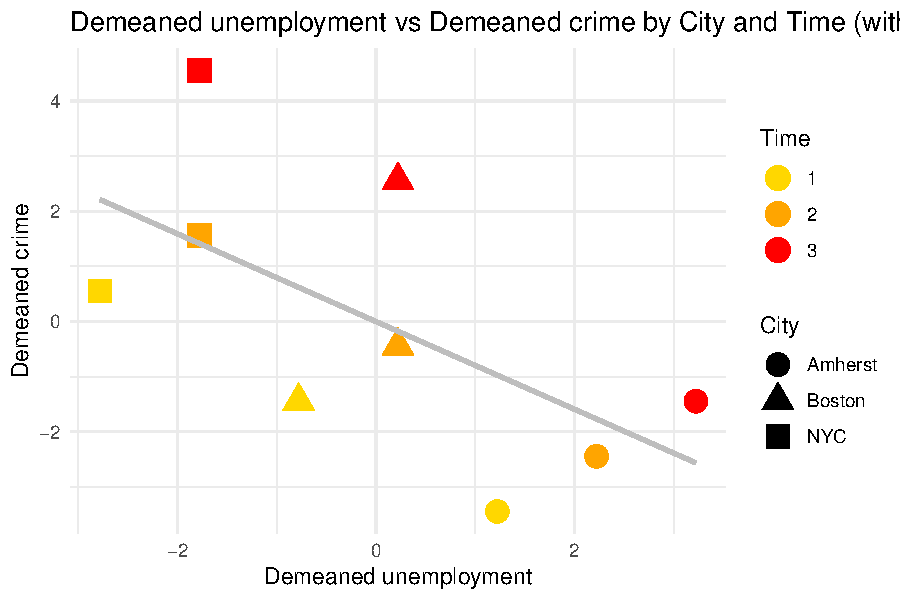
\includegraphics{_main_files/figure-latex/unnamed-chunk-128-1.pdf}

Unemployment over time with horizontal line for between mean values.

\begin{Shaded}
\begin{Highlighting}[]
\NormalTok{X\_BetweenAverage\_T1 }\OtherTok{=}\NormalTok{ df}\SpecialCharTok{$}\NormalTok{X\_BetweenAverage[df}\SpecialCharTok{$}\NormalTok{Time}\SpecialCharTok{==}\StringTok{\textquotesingle{}1\textquotesingle{}}\NormalTok{][}\DecValTok{1}\NormalTok{]}
\NormalTok{X\_BetweenAverage\_T2 }\OtherTok{=}\NormalTok{ df}\SpecialCharTok{$}\NormalTok{X\_BetweenAverage[df}\SpecialCharTok{$}\NormalTok{Time}\SpecialCharTok{==}\StringTok{\textquotesingle{}2\textquotesingle{}}\NormalTok{][}\DecValTok{1}\NormalTok{]}
\NormalTok{X\_BetweenAverage\_T3 }\OtherTok{=}\NormalTok{ df}\SpecialCharTok{$}\NormalTok{X\_BetweenAverage[df}\SpecialCharTok{$}\NormalTok{Time}\SpecialCharTok{==}\StringTok{\textquotesingle{}3\textquotesingle{}}\NormalTok{][}\DecValTok{1}\NormalTok{]}


\FunctionTok{ggplot}\NormalTok{(df, }\FunctionTok{aes}\NormalTok{(}\AttributeTok{x =}\NormalTok{ Time, }\AttributeTok{y =}\NormalTok{ Unemployment, }\AttributeTok{color =} \FunctionTok{factor}\NormalTok{(Time), }\AttributeTok{shape =} \FunctionTok{factor}\NormalTok{(City))) }\SpecialCharTok{+}
  \FunctionTok{geom\_point}\NormalTok{(}\AttributeTok{size =} \DecValTok{5}\NormalTok{) }\SpecialCharTok{+}
  \FunctionTok{scale\_color\_manual}\NormalTok{(}\AttributeTok{values =} \FunctionTok{c}\NormalTok{(}\StringTok{"gold"}\NormalTok{, }\StringTok{"orange"}\NormalTok{, }\StringTok{"red"}\NormalTok{)) }\SpecialCharTok{+}
  \FunctionTok{geom\_smooth}\NormalTok{(}\AttributeTok{method =} \StringTok{"lm"}\NormalTok{, }\AttributeTok{formula =}\NormalTok{ y }\SpecialCharTok{\textasciitilde{}}\NormalTok{ x, }\AttributeTok{se =} \ConstantTok{FALSE}\NormalTok{, }\AttributeTok{color =} \StringTok{"gray"}\NormalTok{) }\SpecialCharTok{+}  \CommentTok{\# Adding the regression line}
  \FunctionTok{geom\_hline}\NormalTok{(}\AttributeTok{yintercept =}\NormalTok{ X\_BetweenAverage\_T1, }\AttributeTok{linetype =} \StringTok{"dashed"}\NormalTok{, }\AttributeTok{color =} \StringTok{"gold"}\NormalTok{) }\SpecialCharTok{+}  \CommentTok{\# Vertical line at the mean of}
  \FunctionTok{geom\_hline}\NormalTok{(}\AttributeTok{yintercept =}\NormalTok{ X\_BetweenAverage\_T2, }\AttributeTok{linetype =} \StringTok{"dashed"}\NormalTok{, }\AttributeTok{color =} \StringTok{"orange"}\NormalTok{) }\SpecialCharTok{+}  \CommentTok{\# Vertical line at the mean of}
  \FunctionTok{geom\_hline}\NormalTok{(}\AttributeTok{yintercept =}\NormalTok{ X\_BetweenAverage\_T3, }\AttributeTok{linetype =} \StringTok{"dashed"}\NormalTok{, }\AttributeTok{color =} \StringTok{"red"}\NormalTok{) }\SpecialCharTok{+}  \CommentTok{\# Vertical line at the mean of}
  \FunctionTok{labs}\NormalTok{(}\AttributeTok{title =} \StringTok{"Time vs Unemployment by City and Time"}\NormalTok{,}
       \AttributeTok{x =} \StringTok{"Time"}\NormalTok{,}
       \AttributeTok{y =} \StringTok{"Unemployment"}\NormalTok{,}
       \AttributeTok{color =} \StringTok{"Time"}\NormalTok{,}
       \AttributeTok{shape =} \StringTok{"City"}\NormalTok{) }\SpecialCharTok{+}
  \FunctionTok{theme\_minimal}\NormalTok{()}
\end{Highlighting}
\end{Shaded}

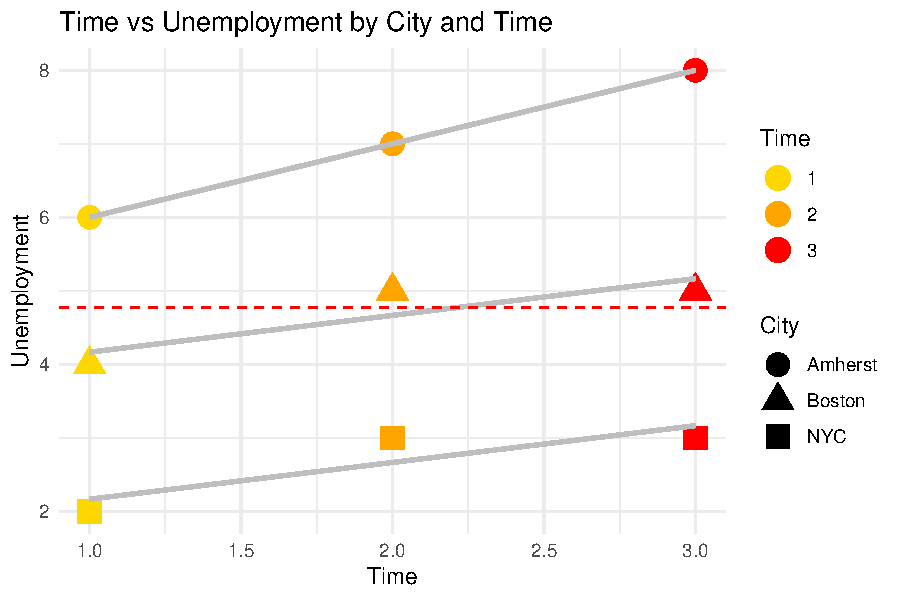
\includegraphics{_main_files/figure-latex/unnamed-chunk-129-1.pdf}

Crime over time with horizontal line for between mean values.

\begin{Shaded}
\begin{Highlighting}[]
\NormalTok{Y\_BetweenAverage\_T1 }\OtherTok{=}\NormalTok{ df}\SpecialCharTok{$}\NormalTok{Y\_BetweenAverage[df}\SpecialCharTok{$}\NormalTok{Time}\SpecialCharTok{==}\StringTok{\textquotesingle{}1\textquotesingle{}}\NormalTok{][}\DecValTok{1}\NormalTok{]}
\NormalTok{Y\_BetweenAverage\_T2 }\OtherTok{=}\NormalTok{ df}\SpecialCharTok{$}\NormalTok{Y\_BetweenAverage[df}\SpecialCharTok{$}\NormalTok{Time}\SpecialCharTok{==}\StringTok{\textquotesingle{}2\textquotesingle{}}\NormalTok{][}\DecValTok{1}\NormalTok{]}
\NormalTok{Y\_BetweenAverage\_T3 }\OtherTok{=}\NormalTok{ df}\SpecialCharTok{$}\NormalTok{Y\_BetweenAverage[df}\SpecialCharTok{$}\NormalTok{Time}\SpecialCharTok{==}\StringTok{\textquotesingle{}3\textquotesingle{}}\NormalTok{][}\DecValTok{1}\NormalTok{]}


\FunctionTok{ggplot}\NormalTok{(df, }\FunctionTok{aes}\NormalTok{(}\AttributeTok{x =}\NormalTok{ Time, }\AttributeTok{y =}\NormalTok{ Crime, }\AttributeTok{color =} \FunctionTok{factor}\NormalTok{(Time), }\AttributeTok{shape =} \FunctionTok{factor}\NormalTok{(City))) }\SpecialCharTok{+}
  \FunctionTok{geom\_point}\NormalTok{(}\AttributeTok{size =} \DecValTok{5}\NormalTok{) }\SpecialCharTok{+}
  \FunctionTok{scale\_color\_manual}\NormalTok{(}\AttributeTok{values =} \FunctionTok{c}\NormalTok{(}\StringTok{"gold"}\NormalTok{, }\StringTok{"orange"}\NormalTok{, }\StringTok{"red"}\NormalTok{)) }\SpecialCharTok{+}
  \FunctionTok{geom\_smooth}\NormalTok{(}\AttributeTok{method =} \StringTok{"lm"}\NormalTok{, }\AttributeTok{formula =}\NormalTok{ y }\SpecialCharTok{\textasciitilde{}}\NormalTok{ x, }\AttributeTok{se =} \ConstantTok{FALSE}\NormalTok{, }\AttributeTok{color =} \StringTok{"gray"}\NormalTok{) }\SpecialCharTok{+}  \CommentTok{\# Adding the regression line}
  \FunctionTok{geom\_hline}\NormalTok{(}\AttributeTok{yintercept =}\NormalTok{ Y\_BetweenAverage\_T1, }\AttributeTok{linetype =} \StringTok{"dotted"}\NormalTok{, }\AttributeTok{color =} \StringTok{"lightgray"}\NormalTok{) }\SpecialCharTok{+}  \CommentTok{\# Vertical line at the mean of}
  \FunctionTok{geom\_hline}\NormalTok{(}\AttributeTok{yintercept =}\NormalTok{ Y\_BetweenAverage\_T2, }\AttributeTok{linetype =} \StringTok{"twodash"}\NormalTok{, }\AttributeTok{color =} \StringTok{"lightgray"}\NormalTok{) }\SpecialCharTok{+}  \CommentTok{\# Vertical line at the mean of}
  \FunctionTok{geom\_hline}\NormalTok{(}\AttributeTok{yintercept =}\NormalTok{ Y\_BetweenAverage\_T3, }\AttributeTok{linetype =} \StringTok{"dashed"}\NormalTok{, }\AttributeTok{color =} \StringTok{"lightgray"}\NormalTok{) }\SpecialCharTok{+}  \CommentTok{\# Vertical line at the mean of}

  \FunctionTok{labs}\NormalTok{(}\AttributeTok{title =} \StringTok{"Time vs Crime by City and Time"}\NormalTok{,}
       \AttributeTok{x =} \StringTok{"Time"}\NormalTok{,}
       \AttributeTok{y =} \StringTok{"Crime"}\NormalTok{,}
       \AttributeTok{color =} \StringTok{"Time"}\NormalTok{,}
       \AttributeTok{shape =} \StringTok{"City"}\NormalTok{) }\SpecialCharTok{+}
  \FunctionTok{theme\_minimal}\NormalTok{()}
\end{Highlighting}
\end{Shaded}

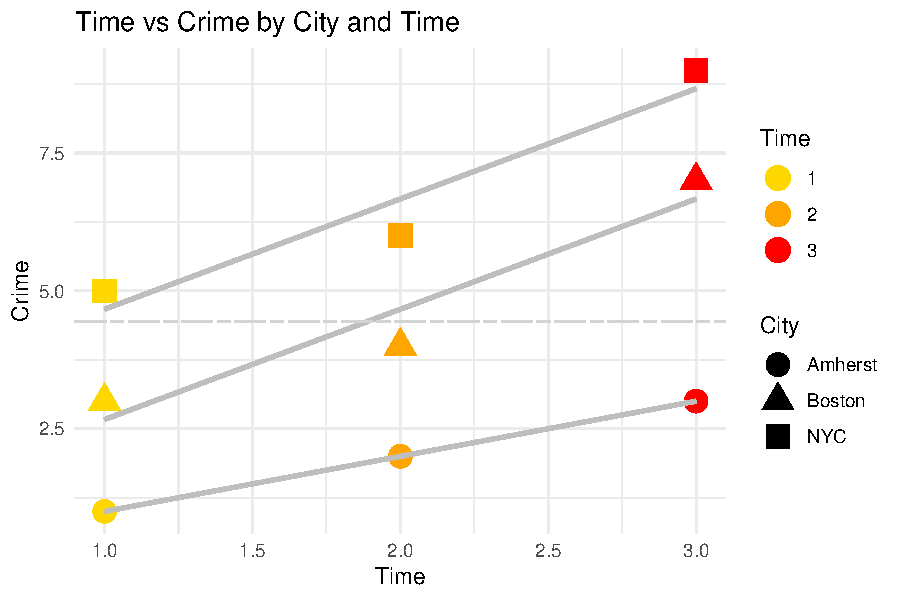
\includegraphics{_main_files/figure-latex/unnamed-chunk-130-1.pdf}

Demeaned unemployment over time with horizontal line for between mean values.

\begin{Shaded}
\begin{Highlighting}[]
\FunctionTok{ggplot}\NormalTok{(df, }\FunctionTok{aes}\NormalTok{(}\AttributeTok{x =}\NormalTok{ Time, }\AttributeTok{y =}\NormalTok{ X\_demeaned\_between, }\AttributeTok{color =} \FunctionTok{factor}\NormalTok{(Time), }\AttributeTok{shape =} \FunctionTok{factor}\NormalTok{(City))) }\SpecialCharTok{+}
  \FunctionTok{geom\_point}\NormalTok{(}\AttributeTok{size =} \DecValTok{5}\NormalTok{) }\SpecialCharTok{+}
  \FunctionTok{scale\_color\_manual}\NormalTok{(}\AttributeTok{values =} \FunctionTok{c}\NormalTok{(}\StringTok{"gold"}\NormalTok{, }\StringTok{"orange"}\NormalTok{, }\StringTok{"red"}\NormalTok{)) }\SpecialCharTok{+}
  \FunctionTok{geom\_smooth}\NormalTok{(}\AttributeTok{method =} \StringTok{"lm"}\NormalTok{, }\AttributeTok{formula =}\NormalTok{ y }\SpecialCharTok{\textasciitilde{}}\NormalTok{ x, }\AttributeTok{se =} \ConstantTok{FALSE}\NormalTok{, }\AttributeTok{color =} \StringTok{"gray"}\NormalTok{) }\SpecialCharTok{+}  \CommentTok{\# Adding the regression line}
  \FunctionTok{labs}\NormalTok{(}\AttributeTok{title =} \StringTok{"Time vs demeaned between unemployment by City and Time"}\NormalTok{,}
       \AttributeTok{x =} \StringTok{"Time"}\NormalTok{,}
       \AttributeTok{y =} \StringTok{"Demeaned unemployment"}\NormalTok{,}
       \AttributeTok{color =} \StringTok{"Time"}\NormalTok{,}
       \AttributeTok{shape =} \StringTok{"City"}\NormalTok{) }\SpecialCharTok{+}
  \FunctionTok{theme\_minimal}\NormalTok{()}
\end{Highlighting}
\end{Shaded}

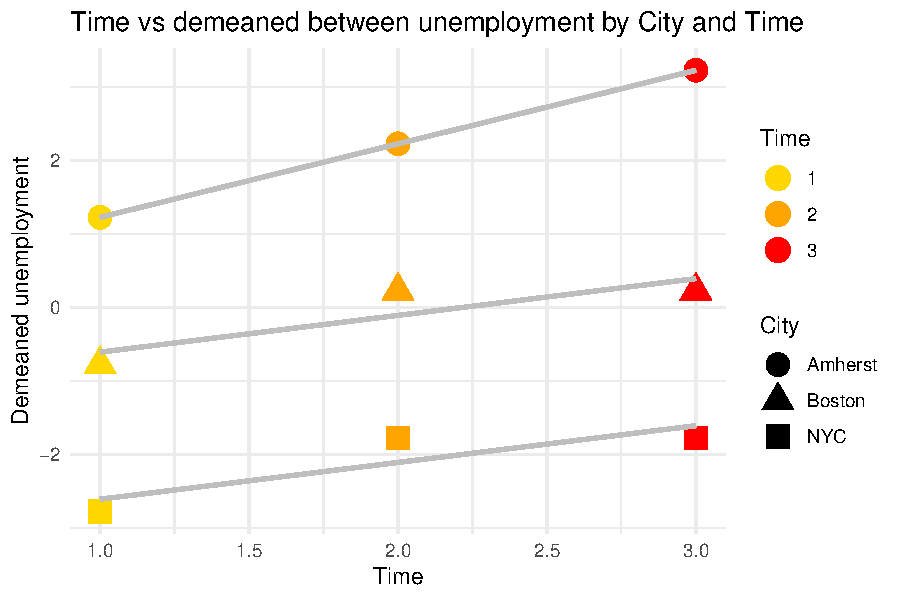
\includegraphics{_main_files/figure-latex/unnamed-chunk-131-1.pdf}

Demeaned crime over time with horizontal line for between mean values.

\begin{Shaded}
\begin{Highlighting}[]
\FunctionTok{ggplot}\NormalTok{(df, }\FunctionTok{aes}\NormalTok{(}\AttributeTok{x =}\NormalTok{ Time, }\AttributeTok{y =}\NormalTok{ Y\_demeaned\_between, }\AttributeTok{color =} \FunctionTok{factor}\NormalTok{(Time), }\AttributeTok{shape =} \FunctionTok{factor}\NormalTok{(City))) }\SpecialCharTok{+}
  \FunctionTok{geom\_point}\NormalTok{(}\AttributeTok{size =} \DecValTok{5}\NormalTok{) }\SpecialCharTok{+}
  \FunctionTok{scale\_color\_manual}\NormalTok{(}\AttributeTok{values =} \FunctionTok{c}\NormalTok{(}\StringTok{"gold"}\NormalTok{, }\StringTok{"orange"}\NormalTok{, }\StringTok{"red"}\NormalTok{)) }\SpecialCharTok{+}
  \FunctionTok{geom\_smooth}\NormalTok{(}\AttributeTok{method =} \StringTok{"lm"}\NormalTok{, }\AttributeTok{formula =}\NormalTok{ y }\SpecialCharTok{\textasciitilde{}}\NormalTok{ x, }\AttributeTok{se =} \ConstantTok{FALSE}\NormalTok{, }\AttributeTok{color =} \StringTok{"gray"}\NormalTok{) }\SpecialCharTok{+}  \CommentTok{\# Adding the regression line}
  \CommentTok{\# scale\_y\_continuous(}
  \CommentTok{\# limits = c(0, 10),}
  \CommentTok{\# breaks = seq(0, 10, by = 1)) +}
  
  \FunctionTok{labs}\NormalTok{(}\AttributeTok{title =} \StringTok{"Time vs demeaned between crime by City and Time"}\NormalTok{,}
       \AttributeTok{x =} \StringTok{"Time"}\NormalTok{,}
       \AttributeTok{y =} \StringTok{"Demeaned crime"}\NormalTok{,}
       \AttributeTok{color =} \StringTok{"Time"}\NormalTok{,}
       \AttributeTok{shape =} \StringTok{"City"}\NormalTok{) }\SpecialCharTok{+}
  \FunctionTok{theme\_minimal}\NormalTok{()}
\end{Highlighting}
\end{Shaded}

\includegraphics{_main_files/figure-latex/unnamed-chunk-132-1.pdf}

Demeaned crime over time with horizontal line for between mean values. \textbf{Very hard to interpret!}

\begin{Shaded}
\begin{Highlighting}[]
\FunctionTok{ggplot}\NormalTok{(df, }\FunctionTok{aes}\NormalTok{(}\AttributeTok{x =}\NormalTok{ X\_demeaned\_between, }\AttributeTok{y =}\NormalTok{ Y\_demeaned\_between)) }\SpecialCharTok{+}
  \FunctionTok{geom\_point}\NormalTok{(}\FunctionTok{aes}\NormalTok{(}\AttributeTok{shape =} \FunctionTok{factor}\NormalTok{(City), }\AttributeTok{color =} \FunctionTok{factor}\NormalTok{(Time)), }\AttributeTok{size =} \DecValTok{5}\NormalTok{) }\SpecialCharTok{+}  \CommentTok{\# Apply shape by City only to points}
  \FunctionTok{scale\_color\_manual}\NormalTok{(}\AttributeTok{values =} \FunctionTok{c}\NormalTok{(}\StringTok{"gold"}\NormalTok{, }\StringTok{"orange"}\NormalTok{, }\StringTok{"red"}\NormalTok{)) }\SpecialCharTok{+}
  \FunctionTok{geom\_smooth}\NormalTok{(}\AttributeTok{method =} \StringTok{"lm"}\NormalTok{, }\AttributeTok{formula =}\NormalTok{ y }\SpecialCharTok{\textasciitilde{}}\NormalTok{ x, }\AttributeTok{se =} \ConstantTok{FALSE}\NormalTok{, }\AttributeTok{color =} \StringTok{"gray"}\NormalTok{) }\SpecialCharTok{+}  \CommentTok{\# Adding the regression line}
  
  \FunctionTok{labs}\NormalTok{(}\AttributeTok{title =} \StringTok{"Demeaned unemployment vs demeaned crime by City and Time (between)"}\NormalTok{,}
       \AttributeTok{x =} \StringTok{"Demeaned unemployment"}\NormalTok{,}
       \AttributeTok{y =} \StringTok{"Demeaned crime"}\NormalTok{,}
       \AttributeTok{color =} \StringTok{"Time"}\NormalTok{,}
       \AttributeTok{shape =} \StringTok{"City"}\NormalTok{) }\SpecialCharTok{+}
  \FunctionTok{theme\_minimal}\NormalTok{()}
\end{Highlighting}
\end{Shaded}

\includegraphics{_main_files/figure-latex/unnamed-chunk-133-1.pdf}

{Missing!! all demeaned (i.e., twoway fixed effects)}

\hypertarget{real-data-2}{%
\subsection{Real data}\label{real-data-2}}

\begin{Shaded}
\begin{Highlighting}[]
\NormalTok{df1 }\OtherTok{\textless{}{-}}\NormalTok{ swissdd}\SpecialCharTok{::}\FunctionTok{get\_nationalvotes}\NormalTok{(}\AttributeTok{geolevel =} \StringTok{"national"}\NormalTok{, }\AttributeTok{from\_date=}\StringTok{"2000{-}03{-}12"}\NormalTok{, }\AttributeTok{to\_date =} \StringTok{"2015{-}06{-}14"}\NormalTok{)}

\NormalTok{df1}\OtherTok{\textless{}{-}}\NormalTok{ df1 }\SpecialCharTok{\%\textgreater{}\%}
  \FunctionTok{select}\NormalTok{(}\StringTok{"stimmbeteiligungInProzent"}\NormalTok{,}\StringTok{"votedate"}\NormalTok{)}
  
\NormalTok{df1 }\OtherTok{\textless{}{-}}\NormalTok{ dplyr}\SpecialCharTok{::}\FunctionTok{rename}\NormalTok{(df1, }\AttributeTok{Y\_National\_BetweenAverage =}\NormalTok{ stimmbeteiligungInProzent, }\AttributeTok{vote\_date =}\NormalTok{ votedate)}


\NormalTok{ballot\_days\_final }\OtherTok{\textless{}{-}} \FunctionTok{readRDS}\NormalTok{(}\StringTok{"Data/replication/data/ballot\_days\_final.rds"}\NormalTok{)  }

\NormalTok{ballot\_days\_final }\OtherTok{\textless{}{-}} \FunctionTok{inner\_join}\NormalTok{(ballot\_days\_final, df1, }\AttributeTok{by=}\StringTok{"vote\_date"}\NormalTok{)  }

\NormalTok{ballot\_days\_final }\OtherTok{\textless{}{-}}\NormalTok{ ballot\_days\_final }\SpecialCharTok{\%\textgreater{}\%}
  \FunctionTok{group\_by}\NormalTok{(muninr) }\SpecialCharTok{\%\textgreater{}\%}
  \FunctionTok{mutate}\NormalTok{(}\AttributeTok{Y\_municipal\_WithinAverage =} \FunctionTok{mean}\NormalTok{(turnout, }\AttributeTok{na.rm =} \ConstantTok{TRUE}\NormalTok{), }
         \AttributeTok{X\_municipal\_WithinAverage =} \FunctionTok{mean}\NormalTok{(postage, }\AttributeTok{na.rm =} \ConstantTok{TRUE}\NormalTok{))}


\NormalTok{ballot\_days\_final }\OtherTok{\textless{}{-}}\NormalTok{ ballot\_days\_final }\SpecialCharTok{\%\textgreater{}\%}
  \FunctionTok{mutate}\NormalTok{(}\AttributeTok{Y\_National\_OverallAverage =} \FunctionTok{mean}\NormalTok{(turnout, }\AttributeTok{na.rm =} \ConstantTok{TRUE}\NormalTok{),}
         \AttributeTok{X\_National\_OverallAverage =} \FunctionTok{mean}\NormalTok{(postage, }\AttributeTok{na.rm =} \ConstantTok{TRUE}\NormalTok{))}

\NormalTok{ballot\_days\_final }\OtherTok{\textless{}{-}}\NormalTok{ ballot\_days\_final }\SpecialCharTok{\%\textgreater{}\%}
  \FunctionTok{group\_by}\NormalTok{(vote\_date) }\SpecialCharTok{\%\textgreater{}\%}
  \FunctionTok{mutate}\NormalTok{(}\AttributeTok{X\_National\_BetweenAverage =} \FunctionTok{mean}\NormalTok{(postage, }\AttributeTok{na.rm =} \ConstantTok{TRUE}\NormalTok{))}
         

\NormalTok{ballot\_days\_final}\OtherTok{\textless{}{-}}\NormalTok{ ballot\_days\_final }\SpecialCharTok{\%\textgreater{}\%}
  \FunctionTok{mutate}\NormalTok{( }\AttributeTok{Y\_demeaned\_within =}\NormalTok{ turnout}\SpecialCharTok{{-}}\NormalTok{Y\_municipal\_WithinAverage,}
          \AttributeTok{Y\_demeaned\_between =}\NormalTok{ turnout}\SpecialCharTok{{-}}\NormalTok{Y\_National\_BetweenAverage,}
          \AttributeTok{Y\_double\_demeaned =}\NormalTok{ turnout}\SpecialCharTok{{-}}\NormalTok{Y\_municipal\_WithinAverage}\SpecialCharTok{{-}}\NormalTok{Y\_National\_BetweenAverage}\SpecialCharTok{+}\NormalTok{Y\_National\_OverallAverage,}
          \AttributeTok{X\_demeaned\_within =}\NormalTok{ postage}\SpecialCharTok{{-}}\NormalTok{X\_municipal\_WithinAverage,}
          \AttributeTok{X\_demeaned\_between =}\NormalTok{ postage}\SpecialCharTok{{-}}\NormalTok{X\_National\_BetweenAverage,}
          \AttributeTok{X\_double\_demeaned =}\NormalTok{ postage}\SpecialCharTok{{-}}\NormalTok{X\_municipal\_WithinAverage}\SpecialCharTok{{-}}\NormalTok{X\_National\_BetweenAverage}\SpecialCharTok{+}\NormalTok{X\_National\_OverallAverage}
\NormalTok{        )}
\end{Highlighting}
\end{Shaded}

Results: One way fixed effects: within

\begin{Shaded}
\begin{Highlighting}[]
\CommentTok{\# One way fixed effects: within}
\NormalTok{OW\_FE\_WI }\OtherTok{\textless{}{-}} \FunctionTok{lm}\NormalTok{(Y\_demeaned\_within }\SpecialCharTok{\textasciitilde{}}\NormalTok{ X\_demeaned\_within }\SpecialCharTok{{-}} \DecValTok{1}\NormalTok{, }\AttributeTok{data =}\NormalTok{ ballot\_days\_final)}
\FunctionTok{summary}\NormalTok{(OW\_FE\_WI)}
\end{Highlighting}
\end{Shaded}

\begin{verbatim}
## 
## Call:
## lm(formula = Y_demeaned_within ~ X_demeaned_within - 1, data = ballot_days_final)
## 
## Residuals:
##    Min     1Q Median     3Q    Max 
## -37.03  -6.53  -0.03   6.67  53.07 
## 
## Coefficients:
##                   Estimate Std. Error t value Pr(>|t|)    
## X_demeaned_within     1.46       0.15    9.73   <2e-16 ***
## ---
## Signif. codes:  0 '***' 0.001 '**' 0.01 '*' 0.05 '.' 0.1 ' ' 1
## 
## Residual standard error: 10.01 on 89319 degrees of freedom
##   (1210 observations deleted due to missingness)
## Multiple R-squared:  0.001059,   Adjusted R-squared:  0.001048 
## F-statistic: 94.67 on 1 and 89319 DF,  p-value: < 2.2e-16
\end{verbatim}

Results: One way fixed effects: between

\begin{Shaded}
\begin{Highlighting}[]
\CommentTok{\# One way fixed effects: between}
\NormalTok{OW\_FE\_BE }\OtherTok{\textless{}{-}} \FunctionTok{lm}\NormalTok{(Y\_demeaned\_between }\SpecialCharTok{\textasciitilde{}}\NormalTok{ X\_demeaned\_between }\SpecialCharTok{{-}} \DecValTok{1}\NormalTok{, }\AttributeTok{data =}\NormalTok{ ballot\_days\_final)}
\FunctionTok{summary}\NormalTok{(OW\_FE\_BE)}
\end{Highlighting}
\end{Shaded}

\begin{verbatim}
## 
## Call:
## lm(formula = Y_demeaned_between ~ X_demeaned_between - 1, data = ballot_days_final)
## 
## Residuals:
##     Min      1Q  Median      3Q     Max 
## -32.706  -6.728  -2.224   2.430  48.172 
## 
## Coefficients:
##                    Estimate Std. Error t value Pr(>|t|)    
## X_demeaned_between   1.3944     0.1132   12.32   <2e-16 ***
## ---
## Signif. codes:  0 '***' 0.001 '**' 0.01 '*' 0.05 '.' 0.1 ' ' 1
## 
## Residual standard error: 7.553 on 89319 degrees of freedom
##   (1210 observations deleted due to missingness)
## Multiple R-squared:  0.001696,   Adjusted R-squared:  0.001685 
## F-statistic: 151.8 on 1 and 89319 DF,  p-value: < 2.2e-16
\end{verbatim}

Results: Two way fixed effects: between

\begin{Shaded}
\begin{Highlighting}[]
\CommentTok{\# Two way fixed effects: between}
\NormalTok{TW\_FE }\OtherTok{\textless{}{-}} \FunctionTok{lm}\NormalTok{(Y\_double\_demeaned }\SpecialCharTok{\textasciitilde{}}\NormalTok{ X\_double\_demeaned }\SpecialCharTok{{-}} \DecValTok{1}\NormalTok{, }\AttributeTok{data =}\NormalTok{ ballot\_days\_final)}
\FunctionTok{summary}\NormalTok{(TW\_FE)}
\end{Highlighting}
\end{Shaded}

\begin{verbatim}
## 
## Call:
## lm(formula = Y_double_demeaned ~ X_double_demeaned - 1, data = ballot_days_final)
## 
## Residuals:
##     Min      1Q  Median      3Q     Max 
## -32.706  -6.728  -2.224   2.430  48.172 
## 
## Coefficients:
##                   Estimate Std. Error t value Pr(>|t|)    
## X_double_demeaned   1.3944     0.1132   12.32   <2e-16 ***
## ---
## Signif. codes:  0 '***' 0.001 '**' 0.01 '*' 0.05 '.' 0.1 ' ' 1
## 
## Residual standard error: 7.553 on 89319 degrees of freedom
##   (1210 observations deleted due to missingness)
## Multiple R-squared:  0.001696,   Adjusted R-squared:  0.001685 
## F-statistic: 151.8 on 1 and 89319 DF,  p-value: < 2.2e-16
\end{verbatim}

{Introduce here the estimation using \emph{plm} }

\hypertarget{week-9}{%
\chapter{Week 9}\label{week-9}}

\hypertarget{exercise-5}{%
\section{Exercise}\label{exercise-5}}

\hypertarget{solution-4}{%
\section{Solution}\label{solution-4}}

\hypertarget{week-10}{%
\chapter{Week 10}\label{week-10}}

\hypertarget{exercise-6}{%
\section{Exercise}\label{exercise-6}}

\hypertarget{solution-5}{%
\section{Solution}\label{solution-5}}

\hypertarget{week-11}{%
\chapter{Week 11}\label{week-11}}

\hypertarget{exercise-7}{%
\section{Exercise}\label{exercise-7}}

\hypertarget{solution-6}{%
\section{Solution}\label{solution-6}}

\hypertarget{week-12}{%
\chapter{Week 12}\label{week-12}}

\hypertarget{exercise-8}{%
\section{Exercise}\label{exercise-8}}

\hypertarget{solution-7}{%
\section{Solution}\label{solution-7}}

\hypertarget{week-13}{%
\chapter{Week 13}\label{week-13}}

\hypertarget{exercise-9}{%
\section{Exercise}\label{exercise-9}}

\hypertarget{solution-8}{%
\section{Solution}\label{solution-8}}

\hypertarget{week-14}{%
\chapter{Week 14}\label{week-14}}

\hypertarget{exercise-10}{%
\section{Exercise}\label{exercise-10}}

\hypertarget{solution-9}{%
\section{Solution}\label{solution-9}}

\hypertarget{potentially-useful-exercises}{%
\chapter{Potentially useful exercises}\label{potentially-useful-exercises}}

\hypertarget{taken-out-from-week-3}{%
\section{Taken out from Week 3}\label{taken-out-from-week-3}}

Parabolic simulated residuals:

\begin{Shaded}
\begin{Highlighting}[]
\NormalTok{CO2\_land}\SpecialCharTok{$}\NormalTok{parab\_norm\_resid}\OtherTok{\textless{}{-}} \SpecialCharTok{{-}}\FloatTok{0.01}\SpecialCharTok{*}\NormalTok{(CO2\_land}\SpecialCharTok{$}\NormalTok{Sim\_ShareAgric\_norm}\SpecialCharTok{{-}}\FunctionTok{mean}\NormalTok{(CO2\_land}\SpecialCharTok{$}\NormalTok{Sim\_ShareAgric\_norm))}\SpecialCharTok{\^{}}\DecValTok{2}\SpecialCharTok{+}\NormalTok{CO2\_land}\SpecialCharTok{$}\NormalTok{Sim\_resid\_norm}
\NormalTok{CO2\_land}\SpecialCharTok{$}\NormalTok{parab\_norm\_resid}\OtherTok{\textless{}{-}}\NormalTok{ CO2\_land}\SpecialCharTok{$}\NormalTok{parab\_norm\_resid}\SpecialCharTok{{-}}\FunctionTok{mean}\NormalTok{(CO2\_land}\SpecialCharTok{$}\NormalTok{parab\_norm\_resid)}


\FunctionTok{ggplot}\NormalTok{(CO2\_land, }\FunctionTok{aes}\NormalTok{(}\AttributeTok{x =}\NormalTok{ Sim\_ShareAgric\_norm, }\AttributeTok{y =}\NormalTok{ parab\_norm\_resid)) }\SpecialCharTok{+}
  \FunctionTok{geom\_point}\NormalTok{() }\SpecialCharTok{+}
  \FunctionTok{geom\_smooth}\NormalTok{(}\AttributeTok{method =} \StringTok{"lm"}\NormalTok{, }\AttributeTok{formula =}\NormalTok{ y }\SpecialCharTok{\textasciitilde{}}\NormalTok{ x, }\AttributeTok{se =} \ConstantTok{FALSE}\NormalTok{, }\AttributeTok{color =} \StringTok{"green"}\NormalTok{) }\SpecialCharTok{+}
  \FunctionTok{theme\_minimal}\NormalTok{() }\SpecialCharTok{+}
  \FunctionTok{theme}\NormalTok{(}\AttributeTok{plot.title =} \FunctionTok{element\_text}\NormalTok{(}\AttributeTok{hjust =} \FloatTok{0.5}\NormalTok{)) }\SpecialCharTok{+}
  \FunctionTok{labs}\NormalTok{(}
    \AttributeTok{x =} \StringTok{"Agricultural Area (\%)"}\NormalTok{,}
    \AttributeTok{y =} \StringTok{"Error"}\NormalTok{,}
    \AttributeTok{title =} \StringTok{"Simulation: of parabolic error"}
\NormalTok{  )}
\end{Highlighting}
\end{Shaded}

\includegraphics{_main_files/figure-latex/unnamed-chunk-138-1.pdf}
What does the behavior of the error tell you about the potential reliability of a regression without quadratic terms?

Data generating process with parabolic residuals:

\begin{Shaded}
\begin{Highlighting}[]
\NormalTok{CO2\_land}\SpecialCharTok{$}\NormalTok{Pred\_TurnOut\_parab\_norm\_resid }\OtherTok{\textless{}{-}}\NormalTok{ CO2\_land}\SpecialCharTok{$}\NormalTok{Pred\_TurnOut\_Determ }\SpecialCharTok{+}\NormalTok{ CO2\_land}\SpecialCharTok{$}\NormalTok{parab\_norm\_resid}



\FunctionTok{ggplot}\NormalTok{(CO2\_land, }\FunctionTok{aes}\NormalTok{(}\AttributeTok{x =}\NormalTok{ Sim\_ShareAgric\_norm, }\AttributeTok{y =}\NormalTok{ Pred\_TurnOut\_parab\_norm\_resid)) }\SpecialCharTok{+}
  \FunctionTok{geom\_point}\NormalTok{() }\SpecialCharTok{+}
  \FunctionTok{geom\_smooth}\NormalTok{(}\AttributeTok{method =} \StringTok{"lm"}\NormalTok{, }\AttributeTok{formula =}\NormalTok{ y }\SpecialCharTok{\textasciitilde{}}\NormalTok{ x, }\AttributeTok{se =} \ConstantTok{FALSE}\NormalTok{, }\AttributeTok{color =} \StringTok{"purple"}\NormalTok{) }\SpecialCharTok{+}
  \FunctionTok{geom\_hline}\NormalTok{(}\AttributeTok{yintercept =} \FunctionTok{mean}\NormalTok{(CO2\_land}\SpecialCharTok{$}\NormalTok{Pred\_TurnOut\_parab\_norm\_resid), }\AttributeTok{linetype =} \StringTok{"dashed"}\NormalTok{, }\AttributeTok{color =} \StringTok{"green"}\NormalTok{) }\SpecialCharTok{+} 
  \FunctionTok{geom\_vline}\NormalTok{(}\AttributeTok{xintercept =}\NormalTok{ mean\_AgricAreaPercent, }\AttributeTok{linetype =} \StringTok{"dashed"}\NormalTok{, }\AttributeTok{color =} \StringTok{"orange"}\NormalTok{) }\SpecialCharTok{+} 
  \FunctionTok{scale\_y\_continuous}\NormalTok{(}\AttributeTok{limits =} \FunctionTok{c}\NormalTok{(}\DecValTok{25}\NormalTok{, }\FunctionTok{max}\NormalTok{(CO2\_land}\SpecialCharTok{$}\NormalTok{Pred\_TurnOut\_Unif, }\AttributeTok{na.rm =} \ConstantTok{TRUE}\NormalTok{))) }\SpecialCharTok{+}  \CommentTok{\#}
  \FunctionTok{theme\_minimal}\NormalTok{() }\SpecialCharTok{+}
  \FunctionTok{theme}\NormalTok{(}\AttributeTok{plot.title =} \FunctionTok{element\_text}\NormalTok{(}\AttributeTok{hjust =} \FloatTok{0.5}\NormalTok{)) }\SpecialCharTok{+}
  \FunctionTok{labs}\NormalTok{(}
    \AttributeTok{x =} \StringTok{"Agricultural Area (\%)"}\NormalTok{,}
    \AttributeTok{y =} \StringTok{"Turn{-}out (\%)"}\NormalTok{,}
    \AttributeTok{title =} \StringTok{"Simulation: deterministic and stochastic model (uniform error)"}
\NormalTok{  )}
\end{Highlighting}
\end{Shaded}

\includegraphics{_main_files/figure-latex/unnamed-chunk-139-1.pdf}
Would using a quadratic term in the regression produce a better fit? Graph the regression line with a quadratic term.

\begin{Shaded}
\begin{Highlighting}[]
\FunctionTok{ggplot}\NormalTok{(CO2\_land, }\FunctionTok{aes}\NormalTok{(}\AttributeTok{x =}\NormalTok{ Sim\_ShareAgric\_norm, }\AttributeTok{y =}\NormalTok{ Pred\_TurnOut\_parab\_norm\_resid)) }\SpecialCharTok{+}
  \FunctionTok{geom\_point}\NormalTok{() }\SpecialCharTok{+}
  \FunctionTok{geom\_smooth}\NormalTok{(}\AttributeTok{method =} \StringTok{"lm"}\NormalTok{, }\AttributeTok{formula =}\NormalTok{ y }\SpecialCharTok{\textasciitilde{}}\NormalTok{ x }\SpecialCharTok{+} \FunctionTok{I}\NormalTok{(x}\SpecialCharTok{\^{}}\DecValTok{2}\NormalTok{), }\AttributeTok{se =} \ConstantTok{FALSE}\NormalTok{, }\AttributeTok{color =} \StringTok{"purple"}\NormalTok{) }\SpecialCharTok{+}
  \FunctionTok{geom\_hline}\NormalTok{(}\AttributeTok{yintercept =} \FunctionTok{mean}\NormalTok{(CO2\_land}\SpecialCharTok{$}\NormalTok{Pred\_TurnOut\_parab\_norm\_resid), }\AttributeTok{linetype =} \StringTok{"dashed"}\NormalTok{, }\AttributeTok{color =} \StringTok{"green"}\NormalTok{) }\SpecialCharTok{+} 
  \FunctionTok{geom\_vline}\NormalTok{(}\AttributeTok{xintercept =}\NormalTok{ mean\_AgricAreaPercent, }\AttributeTok{linetype =} \StringTok{"dashed"}\NormalTok{, }\AttributeTok{color =} \StringTok{"orange"}\NormalTok{) }\SpecialCharTok{+}  
  \FunctionTok{scale\_y\_continuous}\NormalTok{(}\AttributeTok{limits =} \FunctionTok{c}\NormalTok{(}\DecValTok{25}\NormalTok{, }\FunctionTok{max}\NormalTok{(CO2\_land}\SpecialCharTok{$}\NormalTok{Pred\_TurnOut\_Unif, }\AttributeTok{na.rm =} \ConstantTok{TRUE}\NormalTok{))) }\SpecialCharTok{+}  
  \FunctionTok{theme\_minimal}\NormalTok{() }\SpecialCharTok{+}
  \FunctionTok{theme}\NormalTok{(}\AttributeTok{plot.title =} \FunctionTok{element\_text}\NormalTok{(}\AttributeTok{hjust =} \FloatTok{0.5}\NormalTok{)) }\SpecialCharTok{+}
  \FunctionTok{labs}\NormalTok{(}
    \AttributeTok{x =} \StringTok{"Agricultural Area (\%)"}\NormalTok{,}
    \AttributeTok{y =} \StringTok{"Turn{-}out (\%)"}\NormalTok{,}
    \AttributeTok{title =} \StringTok{"Simulation: deterministic and stochastic model (uniform error)"}
\NormalTok{  )}
\end{Highlighting}
\end{Shaded}

\includegraphics{_main_files/figure-latex/unnamed-chunk-140-1.pdf}

\hypertarget{taken-out-from-week-4}{%
\section{Taken out from Week 4}\label{taken-out-from-week-4}}

\begin{Shaded}
\begin{Highlighting}[]
\CommentTok{\# \#\# Interactive Line Plot}
\CommentTok{\# }
\CommentTok{\# *\textless{}span style="color: red;"\textgreater{}Should we exploit this here or somewhere else? I can make it work in R, but not in the book yet. If needed, I can check it out.\textless{}/span\textgreater{}.*}

\CommentTok{\# \# Example data frame}
\CommentTok{\# data \textless{}{-} data.frame(}
\CommentTok{\#   x = rnorm(100),}
\CommentTok{\#   y = rnorm(100)}
\CommentTok{\# )}
\CommentTok{\# }
\CommentTok{\# \# Shiny server function}
\CommentTok{\# server \textless{}{-} function(input, output) \{}
\CommentTok{\#   output$scatterPlot \textless{}{-} renderPlot(\{}
\CommentTok{\#     ggplot(data, aes(x = x, y = y)) +  }
\CommentTok{\#       geom\_point(size = 0) +}
\CommentTok{\#       geom\_abline(intercept = input$intercept, slope = input$slope, color = "red", size = 1)}
\CommentTok{\#   \})}
\CommentTok{\# \}}
\CommentTok{\# }
\CommentTok{\# \# Example data frame}
\CommentTok{\# data \textless{}{-} data.frame(}
\CommentTok{\#   x = rnorm(100),}
\CommentTok{\#   y = rnorm(100)}
\CommentTok{\# )}
\CommentTok{\# }
\CommentTok{\# \# Shiny server function}
\CommentTok{\# server \textless{}{-} function(input, output) \{}
\CommentTok{\#   output$scatterPlot \textless{}{-} renderPlot(\{}
\CommentTok{\#     ggplot(data, aes(x = x, y = y)) +  }
\CommentTok{\#       geom\_point(size = 0) +}
\CommentTok{\#       geom\_abline(intercept = input$intercept, slope = input$slope, color = "red", size = 1)}
\CommentTok{\#   \})}
\CommentTok{\# \}}
\CommentTok{\# }
\CommentTok{\# update.packages(ask = FALSE)}
\CommentTok{\# }
\CommentTok{\# }
\CommentTok{\# library(shiny)}
\CommentTok{\# library(ggplot2)}
\CommentTok{\# }
\CommentTok{\# ui \textless{}{-} fluidPage(}
\CommentTok{\#   titlePanel("Interactive Line Plot"),}
\CommentTok{\#   sidebarLayout(}
\CommentTok{\#     sidebarPanel(}
\CommentTok{\#       sliderInput("intercept", "Intercept:", min = {-}10, max = 10, value = 0),}
\CommentTok{\#       sliderInput("slope", "Slope:", min = {-}10, max = 10, value = 1)}
\CommentTok{\#     ),}
\CommentTok{\#     mainPanel(}
\CommentTok{\#       plotOutput("scatterPlot")}
\CommentTok{\#     )}
\CommentTok{\#   )}
\CommentTok{\# )}
\CommentTok{\# }
\CommentTok{\# server \textless{}{-} function(input, output) \{}
\CommentTok{\#   output$scatterPlot \textless{}{-} renderPlot(\{}
\CommentTok{\#     ggplot(data, aes(x = x, y = y)) +}
\CommentTok{\#       geom\_point(size = 0) +}
\CommentTok{\#       geom\_abline(intercept = input$intercept, slope = input$slope, color = "red", size = 1)}
\CommentTok{\#   \})}
\CommentTok{\# \}}
\CommentTok{\# }
\CommentTok{\# shinyApp(ui = ui, server = server)}
\end{Highlighting}
\end{Shaded}

\hypertarget{simulated-data-3}{%
\subsection{Simulated data}\label{simulated-data-3}}

\begin{Shaded}
\begin{Highlighting}[]
\CommentTok{\# 1. In order to see the logic behind the $R\^{}2$, first estimate the linear regression of \textasciigrave{}LeftToRight\textasciigrave{} on \textasciigrave{}Age\textasciigrave{}. Generate the variable \textasciigrave{}predicted\_LeftToRight\textasciigrave{} with the generated parameters using [\textasciigrave{}predict()\textasciigrave{}](https://www.statology.org/r{-}lm{-}predict/) from the point 3 of the previous section (i.e., the one using real data).Generate the graph \textasciigrave{}predicted\_LeftToRight\textasciigrave{} vs \textasciigrave{}Age\textasciigrave{}.}

\CommentTok{\# Report the regression here.}
\CommentTok{\# \textasciigrave{}\textasciigrave{}\textasciigrave{}\{r\}}
\CommentTok{\# result \textless{}{-} lm(LeftToRight \textasciitilde{} age, data = selects19)}
\CommentTok{\# selects19$predicted\_LeftToRight \textless{}{-} predict(result)}
\CommentTok{\#}
\CommentTok{\# coeffs1 \textless{}{-} coef(result)}
\CommentTok{\# rsq\_sd1 \textless{}{-} summary(result)$r.squared}
\CommentTok{\# cat(\textquotesingle{}The R2 is: \textquotesingle{}, rsq\_sd1, \textquotesingle{}\textbackslash{}n\textbackslash{}nIntercept:\textquotesingle{},unname(coeffs1[1]), \textquotesingle{}\textbackslash{}n\textbackslash{}nSlope:\textquotesingle{}, unname(coeffs1[2]))}
\CommentTok{\# \textasciigrave{}\textasciigrave{}\textasciigrave{}}
\CommentTok{\#}
\CommentTok{\# Report the graph here.}
\CommentTok{\# \textasciigrave{}\textasciigrave{}\textasciigrave{}\{r\}}
\CommentTok{\# \# Calculate means for Y and X}
\CommentTok{\# mean\_LeftRight \textless{}{-} mean(selects19$LeftToRight, na.rm = TRUE)}
\CommentTok{\# mean\_age \textless{}{-} mean(selects19$age, na.rm = TRUE)}
\CommentTok{\#}
\CommentTok{\# \# Create a scatter plot}
\CommentTok{\# ggplot(selects19, aes(x = age, y = predicted\_LeftToRight)) +}
\CommentTok{\#   geom\_smooth(method = "lm", formula = y \textasciitilde{} x, se = FALSE, color = "red") +  \# Adding the regression line}
\CommentTok{\#   geom\_hline(yintercept = mean\_LeftRight, linetype = "dashed", color = "green") +  \# Horizontal line at the mean of y}
\CommentTok{\#   geom\_vline(xintercept = mean\_age, linetype = "dashed", color = "orange") +  \# Vertical line at the mean of x}
\CommentTok{\#   scale\_y\_continuous(}
\CommentTok{\#     limits = c(0, 10),}
\CommentTok{\#     breaks = seq(0, 10, by = 1)}
\CommentTok{\#   ) +}
\CommentTok{\#   theme\_minimal() +}
\CommentTok{\#   theme(}
\CommentTok{\#     plot.title = element\_text(hjust = 0.5), \# Center the plot title}
\CommentTok{\#     panel.grid.major.y = element\_line(color = "grey80", size = 0.5), \# Style for major Y grid lines}
\CommentTok{\#     panel.grid.minor.y = element\_blank() \# Remove minor Y grid lines}
\CommentTok{\#   ) +}
\CommentTok{\#   labs(}
\CommentTok{\#     x = "Age (years)",}
\CommentTok{\#     y = "Political Preferences (left to right)",}
\CommentTok{\#     title = "Scatter plot Age vs. Political Preferences (determ. sim.)"}
\CommentTok{\#   )}
\CommentTok{\#}
\CommentTok{\#}
\CommentTok{\# \textasciigrave{}\textasciigrave{}\textasciigrave{}}
\CommentTok{\#}
\CommentTok{\# 2. Now generate the normally distributed residuals with mean zero and the same variance as the residuals of the model from the previous point.}
\CommentTok{\# \textasciigrave{}\textasciigrave{}\textasciigrave{}\{r\}}
\CommentTok{\# \# Calculate the variance of the residuals}
\CommentTok{\# selects19$residual \textless{}{-} resid(result)}
\CommentTok{\# residual\_sd \textless{}{-} sqrt(var(resid(result)))}
\CommentTok{\#}
\CommentTok{\# \# Set the seed for reproducibility}
\CommentTok{\# set.seed(0)}
\CommentTok{\# selects19$NormResiduals1 \textless{}{-} rnorm(nrow(selects19), mean = 0, sd = residual\_sd)}
\CommentTok{\#}
\CommentTok{\# \textasciigrave{}\textasciigrave{}\textasciigrave{}}
\CommentTok{\#}
\CommentTok{\# 3. Simulate new data using both the deterministic  (i.e., the the parameters estimated immediately above) and stochastic component (i.e., the residuals form the previous point). Graph the simulated data.}
\CommentTok{\# \textasciigrave{}\textasciigrave{}\textasciigrave{}\{r\}}
\CommentTok{\#}
\CommentTok{\# selects19$Sim\_LeftToRight\_Det\_Stoch \textless{}{-} selects19$predicted\_LeftToRight + selects19$NormResiduals1}
\CommentTok{\#}
\CommentTok{\# \#Means for Y and X}
\CommentTok{\# mean\_LeftRight \textless{}{-} mean(selects19$Sim\_LeftToRight\_Det\_Stoch, na.rm = TRUE)}
\CommentTok{\# mean\_age \textless{}{-} mean(selects19$age, na.rm = TRUE)}
\CommentTok{\#}
\CommentTok{\# \# Create a scatter plot}
\CommentTok{\# ggplot(selects19, aes(x = age, y = Sim\_LeftToRight\_Det\_Stoch)) +}
\CommentTok{\#   geom\_point(size = 0) +}
\CommentTok{\#   geom\_smooth(method = "lm", formula = y \textasciitilde{} x, se = FALSE, color = "red") +  \# Adding the regression line}
\CommentTok{\#   geom\_hline(yintercept = mean\_LeftRight, linetype = "dashed", color = "green") +  \# Horizontal line at the mean of y}
\CommentTok{\#   geom\_vline(xintercept = mean\_age, linetype = "dashed", color = "orange") +  \# Vertical line at the mean of x}
\CommentTok{\#   theme\_minimal() +}
\CommentTok{\#   theme(plot.title = element\_text(hjust = 0.5)) +}
\CommentTok{\#   scale\_y\_continuous(}
\CommentTok{\#     limits = c(0, 10),}
\CommentTok{\#     breaks = seq(0, 10, by = 1)) +}
\CommentTok{\#   theme\_minimal() +}
\CommentTok{\#   theme(}
\CommentTok{\#     plot.title = element\_text(hjust = 0.5), \# Center the plot title}
\CommentTok{\#     panel.grid.major.y = element\_line(color = "grey80", size = 0.5), \# Style for major Y grid lines}
\CommentTok{\#     panel.grid.minor.y = element\_blank() \# Remove minor Y grid lines}
\CommentTok{\#   ) +}
\CommentTok{\#   labs(}
\CommentTok{\#     x = "Age (years)",}
\CommentTok{\#     y = "Simulation: Political Preferences (left to right)",}
\CommentTok{\#     title = "Scatter plot Age vs. Political Preferences \textbackslash{}n(determ.\& stoch. sim.)"}
\CommentTok{\#   )}
\CommentTok{\#}
\CommentTok{\# \textasciigrave{}\textasciigrave{}\textasciigrave{}}
\CommentTok{\#}
\CommentTok{\# 4. Now, estimate the regression between the real \textasciigrave{}age\textasciigrave{} and simulated \textasciigrave{}Sim\_LeftToRight\_Det\_Stoch\textasciigrave{}. Once you do that, generate the $R\^{}2$ for the model.}
\CommentTok{\#}
\CommentTok{\# \textasciigrave{}\textasciigrave{}\textasciigrave{}\{r\}}
\CommentTok{\# result \textless{}{-} lm(LeftToRight \textasciitilde{} age, data = selects19)}
\CommentTok{\# rsq\_sd1 \textless{}{-} summary(result)$r.squared}
\CommentTok{\# cat(\textquotesingle{}The R2 is: \textquotesingle{}, rsq\_sd1)}
\CommentTok{\#}
\CommentTok{\# \textasciigrave{}\textasciigrave{}\textasciigrave{}}
\CommentTok{\#}
\CommentTok{\# 5. Repeat the previous three points but use half the standard deviation of the model of point 1. Is the $R\^{}2$ lower now? Why? See [this](https://en.wikipedia.org/wiki/Coefficient\_of\_determination) entry to understand the intuition: pay special attention to the graph with the red and blue squares.}
\CommentTok{\#}
\CommentTok{\# Generate the residuals here.}
\CommentTok{\# \textasciigrave{}\textasciigrave{}\textasciigrave{}\{r\}}
\CommentTok{\# \# Set the seed for reproducibility}
\CommentTok{\# set.seed(0)}
\CommentTok{\# selects19$NormResiduals10 \textless{}{-} rnorm(nrow(selects19), mean = 0, sd = residual\_sd*0.1)}
\CommentTok{\#}
\CommentTok{\# \textasciigrave{}\textasciigrave{}\textasciigrave{}}
\CommentTok{\#}
\CommentTok{\# Simulate new data and graph it here.}
\CommentTok{\# \textasciigrave{}\textasciigrave{}\textasciigrave{}\{r\}}
\CommentTok{\# selects19$Sim\_LeftToRight\_Det\_Stoch\_sd10 \textless{}{-} selects19$predicted\_LeftToRight + selects19$NormResiduals10}
\CommentTok{\#}
\CommentTok{\# \#Means for Y and X}
\CommentTok{\# mean\_LeftRight \textless{}{-} mean(selects19$Sim\_LeftToRight\_Det\_Stoch\_sd10, na.rm = TRUE)}
\CommentTok{\# mean\_age \textless{}{-} mean(selects19$age, na.rm = TRUE)}
\CommentTok{\#}
\CommentTok{\# \# Create a scatter plot}
\CommentTok{\# ggplot(selects19, aes(x = age, y = Sim\_LeftToRight\_Det\_Stoch\_sd10)) +}
\CommentTok{\#   geom\_point(size = 0) +}
\CommentTok{\#   geom\_smooth(method = "lm", formula = y \textasciitilde{} x, se = FALSE, color = "red") +  \# Adding the regression line}
\CommentTok{\#   geom\_hline(yintercept = mean\_LeftRight, linetype = "dashed", color = "green") +  \# Horizontal line at the mean of y}
\CommentTok{\#   geom\_vline(xintercept = mean\_age, linetype = "dashed", color = "orange") +  \# Vertical line at the mean of x}
\CommentTok{\#   scale\_y\_continuous(}
\CommentTok{\#     limits = c(0, 10),}
\CommentTok{\#     breaks = seq(0, 10, by = 1)) +}
\CommentTok{\#   theme\_minimal() +}
\CommentTok{\#   theme(plot.title = element\_text(hjust = 0.5)) +}
\CommentTok{\#   labs(}
\CommentTok{\#     x = "Age (years)",}
\CommentTok{\#     y = "Simulated data (half sd): Political Preferences (left to right)",}
\CommentTok{\#     title = "Scatter plot Age vs. Political Preferences"}
\CommentTok{\#   )}
\CommentTok{\#}
\CommentTok{\# \textasciigrave{}\textasciigrave{}\textasciigrave{}}
\CommentTok{\#}
\CommentTok{\#}
\CommentTok{\# Report the new $R\^{}2$ here:}
\CommentTok{\# \textasciigrave{}\textasciigrave{}\textasciigrave{}\{r\}}
\CommentTok{\# result \textless{}{-} lm(Sim\_LeftToRight\_Det\_Stoch\_sd10 \textasciitilde{} age, data = selects19)}
\CommentTok{\# rsq\_sd10 \textless{}{-} summary(result)$r.squared}
\CommentTok{\# cat(\textquotesingle{}The R2 is: \textquotesingle{}, rsq\_sd10)}
\CommentTok{\#}
\CommentTok{\# \textasciigrave{}\textasciigrave{}\textasciigrave{}}
\CommentTok{\#}
\CommentTok{\# 6. Repeat the previous point but use a hundredth the standard deviation of the model of point 1. Is the $R\^{}2$ lower now? Why?}
\CommentTok{\#}
\CommentTok{\# Generate the residuals here.}
\CommentTok{\# \textasciigrave{}\textasciigrave{}\textasciigrave{}\{r\}}
\CommentTok{\# \# Set the seed for reproducibility}
\CommentTok{\# set.seed(0)}
\CommentTok{\# selects19$NormResiduals100 \textless{}{-} rnorm(nrow(selects19), mean = 0, sd = residual\_sd*0.01)}
\CommentTok{\#}
\CommentTok{\# \textasciigrave{}\textasciigrave{}\textasciigrave{}}
\CommentTok{\#}
\CommentTok{\# Simulate new data and graph it here.}
\CommentTok{\# \textasciigrave{}\textasciigrave{}\textasciigrave{}\{r\}}
\CommentTok{\# selects19$Sim\_LeftToRight\_Det\_Stoch\_hsd \textless{}{-} selects19$predicted\_LeftToRight + selects19$NormResiduals100}
\CommentTok{\#}
\CommentTok{\# \#Means for Y and X}
\CommentTok{\# mean\_LeftRight \textless{}{-} mean(selects19$Sim\_LeftToRight\_Det\_Stoch\_hsd, na.rm = TRUE)}
\CommentTok{\# mean\_age \textless{}{-} mean(selects19$age, na.rm = TRUE)}
\CommentTok{\#}
\CommentTok{\# \# Create a scatter plot}
\CommentTok{\# ggplot(selects19, aes(x = age, y = Sim\_LeftToRight\_Det\_Stoch\_hsd)) +}
\CommentTok{\#   geom\_point(size = 0) +}
\CommentTok{\#   geom\_smooth(method = "lm", formula = y \textasciitilde{} x, se = FALSE, color = "red") +  \# Adding the regression line}
\CommentTok{\#   geom\_hline(yintercept = mean\_LeftRight, linetype = "dashed", color = "green") +  \# Horizontal line at the mean of y}
\CommentTok{\#   geom\_vline(xintercept = mean\_age, linetype = "dashed", color = "orange") +  \# Vertical line at the mean of x}
\CommentTok{\#   scale\_y\_continuous(}
\CommentTok{\#     limits = c(0, 10),}
\CommentTok{\#     breaks = seq(0, 10, by = 1)) +}
\CommentTok{\#   theme\_minimal() +}
\CommentTok{\#   theme(plot.title = element\_text(hjust = 0.5)) +}
\CommentTok{\#   labs(}
\CommentTok{\#     x = "Age (years)",}
\CommentTok{\#     y = "Simulated data (half sd): Political Preferences (left to right)",}
\CommentTok{\#     title = "Scatter plot Age vs. Political Preferences"}
\CommentTok{\#   )}
\CommentTok{\#}
\CommentTok{\# \textasciigrave{}\textasciigrave{}\textasciigrave{}}
\CommentTok{\#}
\CommentTok{\#}
\CommentTok{\# Report the new $R\^{}2$ here:}
\CommentTok{\# \textasciigrave{}\textasciigrave{}\textasciigrave{}\{r\}}
\CommentTok{\# result \textless{}{-} lm(Sim\_LeftToRight\_Det\_Stoch\_hsd \textasciitilde{} age, data = selects19)}
\CommentTok{\# rsq\_sd100 \textless{}{-} summary(result)$r.squared}
\CommentTok{\# cat(\textquotesingle{}The R2 is: \textquotesingle{}, rsq\_sd100)}
\CommentTok{\#}
\CommentTok{\# \textasciigrave{}\textasciigrave{}\textasciigrave{}}
\CommentTok{\#}
\CommentTok{\# 7. Present in a table the $R\^{}2$ for each value of the standard deviation.}
\CommentTok{\# \textasciigrave{}\textasciigrave{}\textasciigrave{}\{r\}}
\CommentTok{\#}
\CommentTok{\# table \textless{}{-} data.frame(}
\CommentTok{\#   SD = c(1, 0.1, 0.01),}
\CommentTok{\#   R2 = c(rsq\_sd1, rsq\_sd10, rsq\_sd100)    \# Replace these with the actual R{-}squared values}
\CommentTok{\# )}
\CommentTok{\#}
\CommentTok{\# print(table)}
\CommentTok{\#}
\CommentTok{\# \textasciigrave{}\textasciigrave{}\textasciigrave{}}
\CommentTok{\# 8. Graph $R\^{}2$ agains the standard deviation fraction. Fit a linear regression line.}
\CommentTok{\# \textasciigrave{}\textasciigrave{}\textasciigrave{}\{r\}}
\CommentTok{\# ggplot(table, aes(x = SD, y = R2)) +}
\CommentTok{\#   geom\_point(size = 0) +}
\CommentTok{\#   geom\_smooth(method = "lm", formula = y \textasciitilde{} x, se = FALSE, color = "green")+}
\CommentTok{\#   theme\_minimal() +}
\CommentTok{\#   theme(plot.title = element\_text(hjust = 0.5)) +}
\CommentTok{\#   labs(}
\CommentTok{\#     x = "Fraction of standard deviation",}
\CommentTok{\#     y = "R2",}
\CommentTok{\#     title = "Relation between R2 and standard deviation of residuals"}
\CommentTok{\#   )}
\CommentTok{\# \textasciigrave{}\textasciigrave{}\textasciigrave{}}
\CommentTok{\# 9. [Optional] Graph $R\^{}2$ against the standard deviation fraction. Fit a regression line with a polynomial of degree 2. The regression line fits the data better. Is the polynomial regression more informative than the linear regression? Why? What lesson does this graph give you in terms of the importance of understanding the theoretical relations between variables beyond what an empirical approach could suggest? What does it teach you regarding the tension between under{-} and over{-}fitting data?}
\CommentTok{\#}
\CommentTok{\# \textasciigrave{}\textasciigrave{}\textasciigrave{}\{r\}}
\CommentTok{\# ggplot(table, aes(x = SD, y = R2)) +}
\CommentTok{\#   geom\_point() +}
\CommentTok{\#   geom\_smooth(method = "lm", formula = y \textasciitilde{} poly(x, 2), se = FALSE, color=\textquotesingle{}green\textquotesingle{}) +}
\CommentTok{\#   theme\_minimal() +}
\CommentTok{\#   theme(plot.title = element\_text(hjust = 0.5)) +}
\CommentTok{\#   labs(}
\CommentTok{\#     x = "Fraction of standard deviation",}
\CommentTok{\#     y = "R2",}
\CommentTok{\#     title = "Relation between R2 and standard deviation of residuals"}
\CommentTok{\#   )}
\CommentTok{\#}
\CommentTok{\#}
\CommentTok{\#}
\CommentTok{\# \textasciigrave{}\textasciigrave{}\textasciigrave{}}
\CommentTok{\# 10. Print the parameters generated in the point 1. Generate the same predictions as in point 1 and 2 but this time multiply the slope\textquotesingle{}s parameter by 5, while keeping the intercept unchanged. Call the resulting predictions \textasciigrave{}predicted\_LeftToRight\_AdjSlope\textasciigrave{} Generate a graph with the regression line for \textasciigrave{}predicted\_LeftToRight\_AdjSlope\textasciigrave{} vs \textasciigrave{}Age\textasciigrave{} and compare it with the graph \textasciigrave{}predicted\_LeftToRight\textasciigrave{} vs \textasciigrave{}Age\textasciigrave{} generated in point 1.}
\CommentTok{\#}
\CommentTok{\# Print here}
\CommentTok{\# \textasciigrave{}\textasciigrave{}\textasciigrave{}\{r\}}
\CommentTok{\# result \textless{}{-} lm(LeftToRight \textasciitilde{} age, data = selects19)}
\CommentTok{\# \# summary(result)}
\CommentTok{\# coeffs \textless{}{-} coef(result)}
\CommentTok{\# cat(\textquotesingle{}Intercept:\textquotesingle{},unname(coeffs[1]), \textquotesingle{}\textbackslash{}n\textbackslash{}nSlope:\textquotesingle{}, unname(coeffs[2]))}
\CommentTok{\# \textasciigrave{}\textasciigrave{}\textasciigrave{}}
\CommentTok{\#}
\CommentTok{\# Predict with the adjusted slope here.}
\CommentTok{\# \textasciigrave{}\textasciigrave{}\textasciigrave{}\{r\}}
\CommentTok{\# selects19$predicted\_LeftToRight\_AdjSlope \textless{}{-} unname(coeffs[1])+(unname(coeffs[2])*5)*selects19$age}
\CommentTok{\# \textasciigrave{}\textasciigrave{}\textasciigrave{}}
\CommentTok{\#}
\CommentTok{\# Generate the graph here.}
\CommentTok{\# \textasciigrave{}\textasciigrave{}\textasciigrave{}\{r\}}
\CommentTok{\# \#Means for Y and X}
\CommentTok{\# mean\_LeftRight \textless{}{-} mean(selects19$predicted\_LeftToRight\_AdjSlope, na.rm = TRUE)}
\CommentTok{\# mean\_age \textless{}{-} mean(selects19$age, na.rm = TRUE)}
\CommentTok{\#}
\CommentTok{\# \# Create a scatter plot}
\CommentTok{\# ggplot(selects19, aes(x = age, y = predicted\_LeftToRight\_AdjSlope)) +}
\CommentTok{\#   geom\_smooth(method = "lm", formula = y \textasciitilde{} x, se = FALSE, color = "red") +  \# Adding the regression line}
\CommentTok{\#   geom\_hline(yintercept = mean\_LeftRight, linetype = "dashed", color = "green") +  \# Horizontal line at the mean of y}
\CommentTok{\#   geom\_vline(xintercept = mean\_age, linetype = "dashed", color = "orange") +  \# Vertical line at the mean of x}
\CommentTok{\#   theme\_minimal() +}
\CommentTok{\#   theme(plot.title = element\_text(hjust = 0.5)) +}
\CommentTok{\#   scale\_y\_continuous(}
\CommentTok{\#     limits = c(0, 15),}
\CommentTok{\#     breaks = seq(0, 20, by = 1)) +}
\CommentTok{\#   theme\_minimal() +}
\CommentTok{\#   theme(}
\CommentTok{\#     plot.title = element\_text(hjust = 0.5), \# Center the plot title}
\CommentTok{\#     panel.grid.major.y = element\_line(color = "grey80", size = 0.5), \# Style for major Y grid lines}
\CommentTok{\#     panel.grid.minor.y = element\_blank() \# Remove minor Y grid lines}
\CommentTok{\#   ) +}
\CommentTok{\#   labs(}
\CommentTok{\#     x = "Age (years)",}
\CommentTok{\#     y = "Political Preferences (left to right)",}
\CommentTok{\#     title = "Scatter plot Age vs. Political Preferences (adj. slope)"}
\CommentTok{\#   )}
\CommentTok{\# \textasciigrave{}\textasciigrave{}\textasciigrave{}}
\CommentTok{\# 11. Add to the deterministic simulation the same stochastic component generated in point 2. Call that variable \textasciigrave{}predicted\_LeftToRight\_AdjSlope\_Stoch\textasciigrave{}. Generate the graph \textasciigrave{}predicted\_LeftToRight\_AdjSlope\_Stoch\textasciigrave{} vs \textasciigrave{}age\textasciigrave{} with a linear regression line. Generate the $R\^{}2$ and compare it to the one generated in point 4. Why is the new $R\^{}2$ higher than the one in point 4?}
\CommentTok{\#}
\CommentTok{\# Report the simulation and the graph here.}
\CommentTok{\# \textasciigrave{}\textasciigrave{}\textasciigrave{}\{r\}}
\CommentTok{\# selects19$predicted\_LeftToRight\_AdjSlope\_Stoch \textless{}{-} selects19$predicted\_LeftToRight\_AdjSlope + selects19$NormResiduals1}
\CommentTok{\#}
\CommentTok{\# \#Means for Y and X}
\CommentTok{\# mean\_LeftRight \textless{}{-} mean(selects19$predicted\_LeftToRight\_AdjSlope\_Stoch, na.rm = TRUE)}
\CommentTok{\# mean\_age \textless{}{-} mean(selects19$age, na.rm = TRUE)}
\CommentTok{\#}
\CommentTok{\# \# Create a scatter plot}
\CommentTok{\# ggplot(selects19, aes(x = age, y = predicted\_LeftToRight\_AdjSlope\_Stoch)) +}
\CommentTok{\#   geom\_point(size = 0) +}
\CommentTok{\#   geom\_smooth(method = "lm", formula = y \textasciitilde{} x, se = FALSE, color = "red") +  \# Adding the regression line}
\CommentTok{\#   geom\_hline(yintercept = mean\_LeftRight, linetype = "dashed", color = "green") +  \# Horizontal line at the mean of y}
\CommentTok{\#   geom\_vline(xintercept = mean\_age, linetype = "dashed", color = "orange") +  \# Vertical line at the mean of x}
\CommentTok{\#   scale\_y\_continuous(}
\CommentTok{\#     limits = c(0, 20),}
\CommentTok{\#     breaks = seq(0, 20, by = 1)) +}
\CommentTok{\#   theme\_minimal() +}
\CommentTok{\#   theme(}
\CommentTok{\#     plot.title = element\_text(hjust = 0.5), \# Center the plot title}
\CommentTok{\#     panel.grid.major.y = element\_line(color = "grey80", size = 0.5), \# Style for major Y grid lines}
\CommentTok{\#     panel.grid.minor.y = element\_blank() \# Remove minor Y grid lines}
\CommentTok{\#   ) +}
\CommentTok{\#   labs(}
\CommentTok{\#     x = "Age (years)",}
\CommentTok{\#     y = "Simulation: Political Preferences (left to right)",}
\CommentTok{\#     title = "Scatter plot Age vs. Political Preferences \textbackslash{}n(determ.\& stoch. sim. with adjusted slope)"}
\CommentTok{\#   )}
\CommentTok{\# \textasciigrave{}\textasciigrave{}\textasciigrave{}}
\CommentTok{\#}
\CommentTok{\# Report the new $R\^{}2$ here:}
\CommentTok{\# \textasciigrave{}\textasciigrave{}\textasciigrave{}\{r\}}
\CommentTok{\# result \textless{}{-} lm(predicted\_LeftToRight\_AdjSlope\_Stoch \textasciitilde{} age, data = selects19)}
\CommentTok{\# rsq\_sd1\_AdjSlope \textless{}{-} summary(result)$r.squared}
\CommentTok{\# cat(\textquotesingle{}The R2 is: \textquotesingle{}, rsq\_sd1\_AdjSlope)}
\CommentTok{\#}
\CommentTok{\# \textasciigrave{}\textasciigrave{}\textasciigrave{}}
\CommentTok{\#}
\CommentTok{\# Report why is the new $R\^{}2$ higher than the one in point 4?}
\CommentTok{\#}
\CommentTok{\# \textasciigrave{}\textasciigrave{}\textasciigrave{}\{r\}}
\CommentTok{\# print(\textquotesingle{}The reason the R2 increased is that, while the distance from each observation to the regression line remained unchainged (i.e., the residual was kept unchanged), by increasing the slope of the generating process, the average distance between each observation and the average observation increased (i.e., Y\textbackslash{}\textquotesingle{}s variance increased). See the graph with the red and blue squares mentioned in point 5.\textquotesingle{})}
\CommentTok{\# \textasciigrave{}\textasciigrave{}\textasciigrave{}}
\CommentTok{\#}
\CommentTok{\# 333333333333}
\CommentTok{\#}
\CommentTok{\#}
\CommentTok{\# 12. Print the parameters generated in the point 1. Generate the same predictions as in point 1 and 2 but this time increase in two units the *intercept\textquotesingle{}s* parameter (not the *slope\textquotesingle{}s* parameter as in the point 10), while keeping the slope unchanged. Call the resulting predictions \textasciigrave{}predicted\_LeftToRight\_AdjSlope\textasciigrave{} Generate a graph with the regression line for \textasciigrave{}predicted\_LeftToRight\_AdjSlope\textasciigrave{} vs \textasciigrave{}Age\textasciigrave{} and compare it with the graph \textasciigrave{}predicted\_LeftToRight\textasciigrave{} vs \textasciigrave{}Age\textasciigrave{} generated in point 1.}
\CommentTok{\#}
\CommentTok{\# Print here}
\CommentTok{\# \textasciigrave{}\textasciigrave{}\textasciigrave{}\{r\}}
\CommentTok{\# result \textless{}{-} lm(predicted\_LeftToRight\_AdjSlope\_Stoch \textasciitilde{} age, data = selects19)}
\CommentTok{\# \# summary(result)}
\CommentTok{\# coeffs12 \textless{}{-} coef(result)}
\CommentTok{\# cat(\textquotesingle{}Intercept:\textquotesingle{},unname(coeffs12[1]), \textquotesingle{}\textbackslash{}n\textbackslash{}nSlope:\textquotesingle{}, unname(coeffs12[2]))}
\CommentTok{\# \textasciigrave{}\textasciigrave{}\textasciigrave{}}
\CommentTok{\#}
\CommentTok{\# Predict with the adjusted slope here.}
\CommentTok{\# \textasciigrave{}\textasciigrave{}\textasciigrave{}\{r\}}
\CommentTok{\# selects19$predicted\_LeftToRight\_AdjIntecept \textless{}{-} unname(coeffs[1]+2)+(unname(coeffs[2]))*selects19$age}
\CommentTok{\# \textasciigrave{}\textasciigrave{}\textasciigrave{}}
\CommentTok{\#}
\CommentTok{\# Generate the graph here.}
\CommentTok{\# \textasciigrave{}\textasciigrave{}\textasciigrave{}\{r\}}
\CommentTok{\# \#Means for Y and X}
\CommentTok{\# mean\_LeftRight \textless{}{-} mean(selects19$predicted\_LeftToRight\_AdjIntecept, na.rm = TRUE)}
\CommentTok{\# mean\_age \textless{}{-} mean(selects19$age, na.rm = TRUE)}
\CommentTok{\#}
\CommentTok{\# \# Create a scatter plot}
\CommentTok{\# ggplot(selects19, aes(x = age, y = predicted\_LeftToRight\_AdjIntecept)) +}
\CommentTok{\#   geom\_smooth(method = "lm", formula = y \textasciitilde{} x, se = FALSE, color = "red") +  \# Adding the regression line}
\CommentTok{\#   geom\_hline(yintercept = mean\_LeftRight, linetype = "dashed", color = "green") +  \# Horizontal line at the mean of y}
\CommentTok{\#   geom\_vline(xintercept = mean\_age, linetype = "dashed", color = "orange") +  \# Vertical line at the mean of x}
\CommentTok{\#   theme\_minimal() +}
\CommentTok{\#   theme(plot.title = element\_text(hjust = 0.5)) +}
\CommentTok{\#   scale\_y\_continuous(}
\CommentTok{\#     limits = c(0, 15),}
\CommentTok{\#     breaks = seq(0, 20, by = 1)) +}
\CommentTok{\#   theme\_minimal() +}
\CommentTok{\#   theme(}
\CommentTok{\#     plot.title = element\_text(hjust = 0.5), \# Center the plot title}
\CommentTok{\#     panel.grid.major.y = element\_line(color = "grey80", size = 0.5), \# Style for major Y grid lines}
\CommentTok{\#     panel.grid.minor.y = element\_blank() \# Remove minor Y grid lines}
\CommentTok{\#   ) +}
\CommentTok{\#   labs(}
\CommentTok{\#     x = "Age (years)",}
\CommentTok{\#     y = "Political Preferences (left to right)",}
\CommentTok{\#     title = "Scatter plot Age vs. Political Preferences (adj. slope)"}
\CommentTok{\#   )}
\CommentTok{\# \textasciigrave{}\textasciigrave{}\textasciigrave{}}
\CommentTok{\# 13. Add to the deterministic simulation the same stochastic component generated in point 2. Call that variable \textasciigrave{}predicted\_LeftToRight\_AdjIntercep\_Stoch\textasciigrave{}. Generate the graph \textasciigrave{}predicted\_LeftToRight\_AdjIntecept\textasciigrave{} vs \textasciigrave{}age\textasciigrave{} with a linear regression line. Generate the $R\^{}2$ and compare it to the one generated in point 4. Why is the new $R\^{}2$ higher than the one in point 4?}
\CommentTok{\#}
\CommentTok{\# Report the simulation and the graph here.}
\CommentTok{\# \textasciigrave{}\textasciigrave{}\textasciigrave{}\{r\}}
\CommentTok{\# selects19$predicted\_LeftToRight\_AdjIntercept\_Stoch \textless{}{-} selects19$predicted\_LeftToRight\_AdjIntecept + selects19$residual}
\CommentTok{\#}
\CommentTok{\# \#Means for Y and X}
\CommentTok{\# mean\_LeftRight \textless{}{-} mean(selects19$predicted\_LeftToRight\_AdjIntercept\_Stoch, na.rm = TRUE)}
\CommentTok{\# mean\_age \textless{}{-} mean(selects19$age, na.rm = TRUE)}
\CommentTok{\#}
\CommentTok{\# \# Create a scatter plot}
\CommentTok{\# ggplot(selects19, aes(x = age, y = predicted\_LeftToRight\_AdjIntercept\_Stoch)) +}
\CommentTok{\#   geom\_point(size = 0) +}
\CommentTok{\#   geom\_smooth(method = "lm", formula = y \textasciitilde{} x, se = FALSE, color = "red") +  \# Adding the regression line}
\CommentTok{\#   geom\_hline(yintercept = mean\_LeftRight, linetype = "dashed", color = "green") +  \# Horizontal line at the mean of y}
\CommentTok{\#   geom\_vline(xintercept = mean\_age, linetype = "dashed", color = "orange") +  \# Vertical line at the mean of x}
\CommentTok{\#   scale\_y\_continuous(}
\CommentTok{\#     limits = c(0, 20),}
\CommentTok{\#     breaks = seq(0, 20, by = 1)) +}
\CommentTok{\#   theme\_minimal() +}
\CommentTok{\#   theme(}
\CommentTok{\#     plot.title = element\_text(hjust = 0.5), \# Center the plot title}
\CommentTok{\#     panel.grid.major.y = element\_line(color = "grey80", size = 0.5), \# Style for major Y grid lines}
\CommentTok{\#     panel.grid.minor.y = element\_blank() \# Remove minor Y grid lines}
\CommentTok{\#   ) +}
\CommentTok{\#   labs(}
\CommentTok{\#     x = "Age (years)",}
\CommentTok{\#     y = "Simulation: Political Preferences (left to right)",}
\CommentTok{\#     title = "Scatter plot Age vs. Political Preferences \textbackslash{}n(determ.\& stoch. sim. with adjusted intercept)"}
\CommentTok{\#   )}
\CommentTok{\# \textasciigrave{}\textasciigrave{}\textasciigrave{}}
\CommentTok{\# Regress the \textasciigrave{}predicted\_LeftToRight\_AdjIntercept\_Stoch\textasciigrave{} on \textasciigrave{}age\textasciigrave{}}
\CommentTok{\# \textasciigrave{}\textasciigrave{}\textasciigrave{}\{r\}}
\CommentTok{\# result \textless{}{-} lm(predicted\_LeftToRight\_AdjIntercept\_Stoch \textasciitilde{} age, data = selects19)}
\CommentTok{\# rsq\_sd1\_AdjIntercept \textless{}{-} summary(result)$r.squared}
\CommentTok{\# coeffs13 \textless{}{-} coef(result)}
\CommentTok{\# cat(\textquotesingle{}Intercept:\textquotesingle{},unname(coeffs13[1]), \textquotesingle{}\textbackslash{}n\textbackslash{}nSlope:\textquotesingle{}, unname(coeffs13[2]))}
\CommentTok{\# \textasciigrave{}\textasciigrave{}\textasciigrave{}}
\CommentTok{\#}
\CommentTok{\# Report the $R\^{}2$ generated in points 2, 11, and 13 here:}
\CommentTok{\# \textasciigrave{}\textasciigrave{}\textasciigrave{}\{r\}}
\CommentTok{\# tableSD1 \textless{}{-} data.frame(}
\CommentTok{\#   LookR2 = c(\textquotesingle{}Point 2\textquotesingle{}, \textquotesingle{}Point 12\textquotesingle{}, \textquotesingle{}Point 13\textquotesingle{}),}
\CommentTok{\#   Model = c(\textquotesingle{}Unchanged\textquotesingle{}, \textquotesingle{}P2 + (slope*5)\textquotesingle{}, \textquotesingle{}P2+(intercept+2)\textquotesingle{}),}
\CommentTok{\#   R2 = c(rsq\_sd1, rsq\_sd1\_AdjSlope, rsq\_sd1\_AdjIntercept),}
\CommentTok{\#   LookParams = c(\textquotesingle{}Point 1\textquotesingle{}, \textquotesingle{}Point 12\textquotesingle{}, \textquotesingle{}Point 13\textquotesingle{}),}
\CommentTok{\#   Intercept = c(unname(coeffs1[1]), unname(coeffs12[1]), unname(coeffs13[1])),}
\CommentTok{\#   Slope = c(unname(coeffs1[2]), unname(coeffs12[2]), unname(coeffs13[2]))}
\CommentTok{\# )}
\CommentTok{\#}
\CommentTok{\#}
\CommentTok{\# print(tableSD1)}
\CommentTok{\#}
\CommentTok{\# \textasciigrave{}\textasciigrave{}\textasciigrave{}}
\CommentTok{\#}
\CommentTok{\# 14. Comparing the $R\^{}2$ and the parameters across the models of points 1, 2, and 3 answer the following questions:}
\CommentTok{\#}
\CommentTok{\#   i. What effect does increasing the slope of the data generating process (while keeping the residuals and intercept unchanged) have on the $R\^{}2$?}
\CommentTok{\# \textasciigrave{}\textasciigrave{}\textasciigrave{}\{r\}}
\CommentTok{\# print(\textquotesingle{}The R2 increases as seen in point 11\textquotesingle{})}
\CommentTok{\# \textasciigrave{}\textasciigrave{}\textasciigrave{}}
\CommentTok{\#}
\CommentTok{\#   ii. What effect does increasing the intercept of the data generating process (while keeping the residuals and slope unchanged) have on the $R\^{}2$?}
\CommentTok{\# \textasciigrave{}\textasciigrave{}\textasciigrave{}\{r\}}
\CommentTok{\# print(\textquotesingle{}The R2 stays unchanged as the distance from each observation to the regression line remained unchainged (i.e., the residual was kept unchanged) as well as the average distance between each observation and the average observation remained unchainged (i.e., Y\textbackslash{}\textquotesingle{}s variance was kept unchanged)\textquotesingle{})}
\CommentTok{\#}
\CommentTok{\# \textasciigrave{}\textasciigrave{}\textasciigrave{}}
\CommentTok{\#}
\CommentTok{\#  iii. What effect does increasing the slope of the data generating process (while keeping the residuals and intercept unchanged) have on the intercept and slope?}
\CommentTok{\# \textasciigrave{}\textasciigrave{}\textasciigrave{}\{r\}}
\CommentTok{\# print(\textquotesingle{}It increases the estimated slope and decreases the intercept.\textquotesingle{})}
\CommentTok{\# \textasciigrave{}\textasciigrave{}\textasciigrave{}}
\CommentTok{\#}
\CommentTok{\#  iv. What effect does increasing the intercept of the data generating process (while keeping the residuals and slope unchanged) have on the intercept and slope?}
\CommentTok{\# \textasciigrave{}\textasciigrave{}\textasciigrave{}\{r\}}
\CommentTok{\# print(\textquotesingle{}It keeps the estimated slope unchanged and the estimated intercept is the same as before the adjustment but increases by the same value that the whole data generating process was modified.\textquotesingle{})}
\end{Highlighting}
\end{Shaded}

\hypertarget{data-transformation}{%
\chapter{Data transformation}\label{data-transformation}}

\hypertarget{week-1-gorilla}{%
\section{Week 1: Gorilla}\label{week-1-gorilla}}

The \href{https://communities.sas.com/t5/Graphics-Programming/Fun-With-SAS-ODS-Graphics-Don-t-Miss-the-Gorilla-in-the-Data/td-p/697286}{original data} of the \href{https://genomebiology.biomedcentral.com/articles/10.1186/s13059-020-02133-w\#citeas}{original paper} was adjusted to put it in a substantively relevant format.

\begin{Shaded}
\begin{Highlighting}[]
\NormalTok{female }\OtherTok{\textless{}{-}} \FunctionTok{read.table}\NormalTok{(}\StringTok{"/Users/fperil/Documents/0\_IPZ/2023\_2/Leemann{-}QuantMethods/QuantitativeMethods/OriginalData/f.txt"}\NormalTok{, }\AttributeTok{header =} \ConstantTok{TRUE}\NormalTok{, }\AttributeTok{sep =} \StringTok{"}\SpecialCharTok{\textbackslash{}t}\StringTok{"}\NormalTok{)}
\NormalTok{male }\OtherTok{\textless{}{-}} \FunctionTok{read.table}\NormalTok{(}\StringTok{"/Users/fperil/Documents/0\_IPZ/2023\_2/Leemann{-}QuantMethods/QuantitativeMethods/OriginalData/m.txt"}\NormalTok{, }\AttributeTok{header =} \ConstantTok{TRUE}\NormalTok{, }\AttributeTok{sep =} \StringTok{"}\SpecialCharTok{\textbackslash{}t}\StringTok{"}\NormalTok{)}

\NormalTok{male }\OtherTok{\textless{}{-}}\NormalTok{ dplyr}\SpecialCharTok{::}\FunctionTok{rename}\NormalTok{(male, }\AttributeTok{ScreenTime =}\NormalTok{ steps, }\AttributeTok{ClosenessPopulistParty=}\NormalTok{bmi  )}

\NormalTok{female }\OtherTok{\textless{}{-}}\NormalTok{ dplyr}\SpecialCharTok{::}\FunctionTok{rename}\NormalTok{(female, }\AttributeTok{ScreenTime =}\NormalTok{ steps, }\AttributeTok{ClosenessPopulistParty=}\NormalTok{bmi  )}

\NormalTok{female }\OtherTok{\textless{}{-}}\NormalTok{female }\SpecialCharTok{\%\textgreater{}\%}
  \FunctionTok{mutate}\NormalTok{(}\AttributeTok{ClosenessPopulistParty=} \DecValTok{10}\SpecialCharTok{*}\NormalTok{(female}\SpecialCharTok{$}\NormalTok{ClosenessPopulistParty}\SpecialCharTok{{-}}\FunctionTok{min}\NormalTok{(female}\SpecialCharTok{$}\NormalTok{ClosenessPopulistParty))}\SpecialCharTok{/}\NormalTok{(}\FunctionTok{max}\NormalTok{(ClosenessPopulistParty)}\SpecialCharTok{{-}}\FunctionTok{min}\NormalTok{(female}\SpecialCharTok{$}\NormalTok{ClosenessPopulistParty)))}

\NormalTok{male }\OtherTok{\textless{}{-}}\NormalTok{male }\SpecialCharTok{\%\textgreater{}\%}
  \FunctionTok{mutate}\NormalTok{(}\AttributeTok{ClosenessPopulistParty=} \DecValTok{10}\SpecialCharTok{*}\NormalTok{(male}\SpecialCharTok{$}\NormalTok{ClosenessPopulistParty}\SpecialCharTok{{-}}\FunctionTok{min}\NormalTok{(male}\SpecialCharTok{$}\NormalTok{ClosenessPopulistParty))}\SpecialCharTok{/}\NormalTok{(}\FunctionTok{max}\NormalTok{(male}\SpecialCharTok{$}\NormalTok{ClosenessPopulistParty)}\SpecialCharTok{{-}}\FunctionTok{min}\NormalTok{(male}\SpecialCharTok{$}\NormalTok{ClosenessPopulistParty)))}


\FunctionTok{write.table}\NormalTok{(female, }\StringTok{"Data/f.txt"}\NormalTok{, }\AttributeTok{sep =} \StringTok{";"}\NormalTok{)}
\FunctionTok{write.table}\NormalTok{(male, }\StringTok{"Data/m.txt"}\NormalTok{, }\AttributeTok{sep =} \StringTok{";"}\NormalTok{)}
\end{Highlighting}
\end{Shaded}

\hypertarget{week-4-restricted-variables-from-selects}{%
\section{Week 4: restricted variables from SELECTS}\label{week-4-restricted-variables-from-selects}}

\begin{Shaded}
\begin{Highlighting}[]
\NormalTok{selects19 }\OtherTok{\textless{}{-}} \FunctionTok{read.csv}\NormalTok{(}\StringTok{"/Users/fperil/Documents/0\_IPZ/2023\_2/Leemann{-}QuantMethods/QuantitativeMethods/OriginalData/SELECTS 2019/1179\_Selects2019\_PES\_Data\_v1.1.0.csv"}\NormalTok{, }\AttributeTok{header =} \ConstantTok{TRUE}\NormalTok{)}

\NormalTok{selects19 }\OtherTok{\textless{}{-}}\NormalTok{ selects19 }\SpecialCharTok{\%\textgreater{}\%}
  \FunctionTok{select}\NormalTok{(sex, age, }\FunctionTok{matches}\NormalTok{(}\StringTok{"f15200"}\NormalTok{), f20221) }\SpecialCharTok{\%\textgreater{}\%}
  \FunctionTok{filter}\NormalTok{(}\SpecialCharTok{!}\FunctionTok{is.na}\NormalTok{(selects19}\SpecialCharTok{$}\NormalTok{sex) }\SpecialCharTok{\&} \SpecialCharTok{!}\FunctionTok{is.na}\NormalTok{(selects19}\SpecialCharTok{$}\NormalTok{age) }\SpecialCharTok{\&} \SpecialCharTok{!}\FunctionTok{is.na}\NormalTok{(selects19}\SpecialCharTok{$}\NormalTok{f15200) }\SpecialCharTok{\&} \SpecialCharTok{!}\FunctionTok{is.na}\NormalTok{(selects19}\SpecialCharTok{$}\NormalTok{f20221))  }\CommentTok{\# Remove rows where x or y is NA}

\NormalTok{selects19}\SpecialCharTok{$}\NormalTok{f15200 }\OtherTok{\textless{}{-}} \FunctionTok{as.numeric}\NormalTok{(selects19}\SpecialCharTok{$}\NormalTok{f15200)}

\FunctionTok{write.table}\NormalTok{(selects19, }\AttributeTok{file =} \StringTok{"Data/SELECTS 2019/data.csv"}\NormalTok{, }\AttributeTok{sep =} \StringTok{","}\NormalTok{, }\AttributeTok{row.names =} \ConstantTok{FALSE}\NormalTok{)}
\end{Highlighting}
\end{Shaded}


  \bibliography{book.bib,packages.bib}

\end{document}
